%!TeX program=pdflatex
%!TeX encoding=utf8
%!TeX spellcheck = en_US

\gdef\doctype{extbook}
\documentclass[a4paper,appendixprefix,pdfusetitle,twocolumn,fontsize=12pt,DIV=calc,12pt,final,utf8]{\doctype} %scrbook
% add attachdocs to attach all documents
% add openany to avoid empty pages

% add encoding spec
\usepackage[utf8]{inputenc}
\usepackage[T1]{fontenc}

% fix some fonts
\usepackage{sansmath}                  % Maths without serifes
\usepackage{microtype}                 % better text distribution in lines

% Workarround for book
\makeatletter
\newcommand\subtitle[1]{\gdef\@subtitle{#1}}
\makeatother

\PassOptionsToPackage{table,svgnames}{xcolor}

% enable breakable URLS
\PassOptionsToPackage{hyphens}{url}

\usepackage{colortbl}

% Make C&P work
\usepackage{cmap}

% Some index related settings
%\usepackage{imakeidx}
%\makeindex[columns=3, title=Alphabetical Index]
\usepackage{makeidx}
\makeindex

\makeatletter
\let\inserttitle\@title
\makeatother

%\makeatletter
%\def\title#1{\gdef\@title{#1}\gdef\thetitle{#1}}
%\makeatother

\PassOptionsToPackage{final}{graphicx}

\usepackage{tikz}
\usetikzlibrary{calc,positioning,arrows.meta,backgrounds,shapes.geometric,shadows.blur}
\tikzset{background rectangle/.style={fill=black!10}, show background rectangle}

\usepackage[draft=false,automark]{scrlayer-scrpage}
% and make some nice page headers
\automark{part}
\automark*{chapter}
\clearpairofpagestyles
\ihead{\headmark}
\ohead{\pagemark}

\setheadsepline{0.55pt}
\setkomafont{headsepline}{\color{black}}
\definecolor{head}{rgb}{0.01, 0.28, 1.0}

\gdef\thetitle{MessageVortex}
\title{\thetitle}
\gdef\thesubtitle{Transport Independent, Unobservable, and Unlinkable Messaging}
\subtitle{\thesubtitle}
\author{Martin Gwerder (06-073-787)}
%\date{\gitAuthorDate}
\gdef\myabstract{
	In this thesis, we introduce an unobservable message anonymization protocol named MessageVortex. It is based on the zero-trust principle, has a distributed peer-to-peer (P2P) architecture, and avoids central aspects such as fixed infrastructures within a global network. It scores over existing work by blending its traffic into suitable standard transport protocols like SMTP, making it next to impossible to block it without significantly affecting regular users of the transport medium. No additional protocol-specific infrastructure is required in public networks and allows a sender to control all aspects of a message, such as the degree of anonymity, timing, and redundancy of the message transport, without disclosing any of these details to routing or transporting nodes. We have made our prototype implementation publicly available and added an RFC-style document that contains all necessary information to build a MessageVortex node, see https://messagevortex.net/.
}
\makeatother

% for PDF/A generation
\makeatletter
\@ifclasswith{\doctype}{attachdocs}{
	\usepackage[
	  pdfencoding=unicode,
	  psdextra,
	  bookmarks,
	  hyperindex,
	  hyperfigures,
	  pdfpagelabels,
	  final]{hyperref}
}{
	\typeout{INFO: ======================}
	\typeout{INFO: creating PDF/A}
	\typeout{INFO: ======================}
	\PassOptionsToPackage{
  	  pdfencoding=unicode,
	  psdextra,
	  bookmarks,
	  hyperindex,
	  hyperfigures,
	  pdfpagelabels,
	  final}{hyperref}
	\usepackage[a-3b]{pdfx}
	\catcode30=12
}
\makeatother

% XMP support 
\RequirePackage{xmpincl}
%\includexmp{messageVortex}
\usepackage{hyperxmp}

%enable hyperlinks
\makeatletter
\hypersetup{	
	pdfpagelayout=TwoPageRight,
	linktoc=all,
	breaklinks=true,
	hidelinks,
	pdfstartview=Fit,
	pdfauthor={\author},
	pdftitle={\thetitle - \thesubtitle},
	pdflang=en,
	pdfsubject={\myabstract},
	pdfkeywords={Messaging, Anonymity, SMTP, Message Vortex},
	pdfcontactemail={martin.gwerder@fhnw.ch},
	pdflicenseurl={http://creativecommons.org/licenses/by-nc-nd/3.0/ch/},
	pdfcopyright={Creative Commons Attribution-NonCommercial-NoDerivatives 3.0 Switzerland (CC BY-NC-ND 3.0 CH)}
}
\makeatother

% enable superscript  for 1st, 2nd, 3rd etc.
\usepackage[super]{nth}

% extended width for toc page numbers
\usepackage[titles]{tocloft}
\cftsetpnumwidth{3em}
% Format appendix
\setlength{\cftchapnumwidth}{16pt}%
%\renewcommand{\cftpartpresnum}{\partname\hspace{13pt}}
\renewcommand{\cftchappresnum}{\chaptername\hspace{5pt}}
\renewcommand{\cftchapaftersnum}{\hspace{5pt}}

% Extract filename from path
\makeatletter
\DeclareRobustCommand{\filenameExtract}[1]{%
 \begingroup
  % \lstname seems to change hyphens into \textendash
  \def\textendash{-}%
  \filename@parse{#1}%
  \edef\filename@base{\detokenize\expandafter{\filename@base}}%
  \texttt{\filename@base.\filename@ext}%
 \endgroup
}
\makeatother

% PDF/a measures
% embed color profile 
%\immediate\pdfobj stream attr{/N 3} file{sRGB_IEC61966-2-1_black_scaled.ICC}
%\pdfcatalog{%
%	/OutputIntents [ <<
%	/Type /OutputIntent
%	/S/GTS_PDFA1
%	/DestOutputProfile \the\pdflastobj\space 0 R
%	/OutputConditionIdentifier (sRGB IEC61966-2-1 black scaled)
%	/Info(sRGB IEC61966-2-1 black scaled)
%	>> ]
%}
% map glyphs 
\input{glyphtounicode.tex}
\input{glyphtounicode-cmr.tex}
\pdfgentounicode=1
% deactivate LZW compression
\pdfobjcompresslevel=0
\pdfinclusioncopyfonts=1

% Table environments
\usepackage{booktabs}
\newcommand*\rot{\rotatebox{90}}

\usepackage{xstring}

\usepackage{pdfsync} 

%\usepackage{MnSymbol} % required for the arrow

%\usepackage{underscore}

% No new page for chapters
\usepackage{etoolbox}
\makeatletter
\patchcmd{\chapter}{\if@openright\cleardoublepage\else\clearpage\fi}{}{}{}
\makeatother

% hidden sections and subsections
\newcommand{\hiddensubsubsection}[1]{
	\stepcounter{subsubsection}
	\subsection*{\arabic{chapter}.\arabic{section}.\arabic{subsection}.\arabic{subsubsection}\hspace{1em}{#1}}
}
\newcommand{\hiddensubsection}[1]{
	\stepcounter{subsection}
	\subsection*{\arabic{chapter}.\arabic{section}.\arabic{subsection}\hspace{1em}{#1}}
}
\newcommand{\hiddensection}[1]{
	\stepcounter{section}
	\subsection*{\arabic{chapter}.\arabic{section}\hspace{1em}{#1}}
}

% titlepage geometry change
\usepackage[paper=a4paper,top=2cm,bottom=2cm,inner=3.1cm,outer=2.2cm]{geometry}% http://ctan.org/pkg/geometry

% Pagestyles
% For formulae in twocolumn
\usepackage{mathtools}
\usepackage{amsmath}
\usepackage{amssymb}
\usepackage{cuted}

% line breaking in math mode
%\usepackage{scrhack}

\usepackage[autocite=superscript,
            backref=true,
            backend=biber,
            hyperref=true,
            url=true,
            isbn=true,
            maxcitenames=3,
            minbibnames=1,
            maxbibnames=300,
            bibencoding=utf8,
            block=none,
            sorting=anyt]{biblatex}

%\bibstyle{alphadin}
\addbibresource{messageVortex.bib}
%\addbibresource{inc/bib/unclassified/Anonbib/anonbib}
\usepackage{csquotes}

% For Multipage listing in appendix
\usepackage[final]{listings}
\usepackage{caption}
\usepackage[framemethod=tikz]{mdframed}
\usepackage[many]{tcolorbox}
\tcbuselibrary{listings}
\usepackage{multicol}% for multiple column listings
\usepackage{float} % for defining floats
\newfloat{lstfloat}{htbp}{lop}
\floatname{lstfloat}{Listing}
\def\lstfloatautorefname{Listing} % needed for hyperref/auroref
\lstset{commentstyle=\color{darkgray}}
\lstdefinelanguage[]{asn.1}{
	keywords={DEFINITIONS,SEQUENCE,OCTET,INTEGER,BEGIN,END,OPTIONAL,STRING},
	sensitive=true,
	comment=[l]{--}, % l is for line comment
	string=[b]", % defines that strings are enclosed in double quotes
} 


% enable raggedright in tables
\usepackage{array}
% for diagonal divided cells in tables
\usepackage{makecell}
\renewcommand\theadfont{\bfseries}

% footnotes for tables
\usepackage{tablefootnote}
%\makesavenoteenv{tabular}
%\makesavenoteenv{table}

% enable placement of floating images
\usepackage{float}

%enable page spanning tables
\usepackage{supertabular}

% Link above tables and figures
%\usepackage[hypcap]{caption}

% support repetitive footnotes
\usepackage{fixfoot}

% Support for algorithms
\usepackage{amsmath}
\usepackage{algorithm}
\usepackage{algpseudocode}
\algnewcommand{\AbstractFunction}[2]{\State \textbf{abstract function} \textproc{#1}(#2) \{\ldots\};}%
\algdef{SE}% flags used internally to indicate we're defining a new block statement
[OBJECT]% new block type, not to be confused with loops or if-statements
{Object}% "\Struct{name}" will indicate the start of the struct declaration
{EndObject}% "\EndStruct" ends the block indent
[1]% There is one argument, which is the name of the data structure
{\textbf{object} \textsc{#1}}% typesetting of the start of a struct
{\textbf{end object}}% typesetting the end of the struct
%set font size of algorithms
\makeatletter
\renewcommand{\ALG@beginalgorithmic}{\scriptsize}
\makeatother
% boolean operators
\algnewcommand\And{~\textbf{and}~}
\algnewcommand\Or{~\textbf{or}~}
\algnewcommand\Not{~\neg~}
\algnewcommand\Throw{\State \textbf{throw}~}
\algnewcommand{\LineComment}[1]{\State {\ttfamily\textcolor{blue}{\(\triangleright\) #1}}}


\usepackage{caption}
\newcounter{nalg}[chapter] % defines algorithm counter for chapter-level
\renewcommand{\thenalg}{\thechapter .\arabic{nalg}} %defines appearance of the algorithm counter
\DeclareCaptionLabelFormat{algocaption}{Algorithm \thenalg} % defines a new caption label as Algorithm x.y
% Allow pagebreak in algorithms
\makeatletter
\newenvironment{breakablealgorithm}
{% \begin{breakablealgorithm}
	\begin{center}
		\refstepcounter{algorithm}% New algorithm
		\hrule height.8pt depth0pt \kern2pt% \@fs@pre for \@fs@ruled
		\renewcommand{\caption}[2][\relax]{% Make a new \caption
			{\raggedright\textbf{\ALG@name~\thealgorithm} ##2\par}%
			\ifx\relax##1\relax % #1 is \relax
			\addcontentsline{loa}{algorithm}{\protect\numberline{\thealgorithm}##2}%
			\else % #1 is not \relax
			\addcontentsline{loa}{algorithm}{\protect\numberline{\thealgorithm}##1}%
			\fi
			\kern2pt\hrule\kern2pt
		}
	}{% \end{breakablealgorithm}
		\kern2pt\hrule\relax% \@fs@post for \@fs@ruled
	\end{center}
}
\makeatother
%linebreak in algorithms 
\algrenewcommand{\algorithmicreturn}{\State \textbf{return}}
\newcommand\CONDITION[2]%
{\begin{tabular}[t]{@{}l@{}l@{}}
		#1&#2
	\end{tabular}%
}
\algdef{SE}[WHILE]{While}{EndWhile}[1]%
{\algorithmicwhile\ \CONDITION{#1}{\ \algorithmicdo}}%
{\algorithmicend\ \algorithmicwhile}
\algdef{SE}[FOR]{For}{EndFor}[1]%
{\algorithmicfor\ \CONDITION{#1}{\ \algorithmicdo}}%
{\algorithmicend\ \algorithmicfor}
\algdef{S}[FOR]{ForAll}[1]%
{\algorithmicforall\ \CONDITION{#1}{\ \algorithmicdo}}
\algdef{SE}[REPEAT]{Repeat}{Until}{\algorithmicrepeat}[1]%
{\algorithmicuntil\ \CONDITION{#1}{}}
\algdef{SE}[IF]{If}{EndIf}[1]%
{\algorithmicif\ \CONDITION{#1}{\ \algorithmicthen}}%
{\algorithmicend\ \algorithmicif}%
\algdef{C}[IF]{IF}{ElsIf}[1]%
{\algorithmicelse\ \algorithmicif\ \CONDITION{#1}{\ \algorithmicthen}}
%references to functions
\makeatletter
\renewcommand{\Function}[2]{%
	\csname ALG@cmd@\ALG@L @Function\endcsname{#1}{#2}%
	\def\jayden@currentfunction{#1}%
}
\newcommand{\funclabel}[1]{%
	\@bsphack
	\protected@write\@auxout{}{%
		\string\newlabel{#1}{{\jayden@currentfunction}{\thepage}{}{}{}}%
	}%
	\@esphack
}
\renewcommand{\Procedure}[2]{%
	\csname ALG@cmd@\ALG@L @Procedure\endcsname{#1}{#2}%
	\def\jayden@currentprocedure{#1}%
}
\newcommand{\proclabel}[1]{%
	\@bsphack
	\protected@write\@auxout{}{%
		\string\newlabel{#1}{{\jayden@currentprocedure}{\thepage}{}{}{}}%
	}%
	\@esphack
}
\newcommand{\funcref}[1]{\@bsphack\textproc{\ref{#1}}\@esphack}
\makeatother
% Euler number
\newcommand{\euler}{\mathrm{e}}


%\lstnewenvironment{algorithm}[1][] %defines the algorithm listing environment
%{   
%	\refstepcounter{nalg} %increments algorithm number
%	\captionsetup{labelformat=algocaption,labelsep=colon} %defines the caption setup for: it ises label format as the declared caption label above and makes label and caption text to be separated by a ':'
%	\lstset{ %this is the stype
%		mathescape=true,
%		frame=tB,
%		numbers=left, 
%		numberstyle=\tiny,
%		basicstyle=\scriptsize, 
%		keywordstyle=\color{black}\bfseries\em,
%		keywords={,input, output, return, datatype, function, in, if, else, foreach, while, begin, end, } %add the keywords you want, or load a language as Rubens explains in his comment above.
%		numbers=left,
%		xleftmargin=.04\textwidth,
%		#1 % this is to add specific settings to an usage of this environment (for instnce, the caption and referable label)
%	}
%}
%{}
% Document annotations
\usepackage[nomargin]{fixme}
\fxsetup{layout=pdfnote}

%enable attached files
\usepackage[color=black]{attachfile}
\usepackage{embedfile}
\usepackage{hypgotoe}

% graphs
\usepackage{pgfplots}

%enable word separation
\usepackage[english]{babel}

% enable nice references
\usepackage{fancyref}

% format appendix
\usepackage{bookmark}
\usepackage[]{appendix} %enable appendix 

\let\oldappendices\appendices
\renewcommand{\appendices}{%
	\oldappendices
	\bookmarksetupnext{level=-1}
	\addtocontents{toc}{\protect\renewcommand\protect\cftpartpresnum{}}
	\addcontentsline{toc}{part}{Appendices}
	\addtocontents{toc}{\protect\renewcommand\protect\cftchappresnum{}%
		\protect\setlength\protect\cftchapnumwidth{15pt}}%
}

% citations
%\usepackage{cite}

%fonts for comparison table 
\usepackage{pifont,wasysym,fontawesome,txfonts,marvosym,fontawesome}

% colored tables 
\usepackage{colortbl}


% Sans serif font for the whole document
\renewcommand{\familydefault}{\sfdefault}
\usepackage[T1]{fontenc}
\usepackage{times}

\usepackage{amsmath}

% No paragraph indentation
\setlength\parindent{0pt} 
\setlength\parskip{6pt} 

% For coments and similar
\usepackage{verbatim}

% For Page background color
\usepackage{afterpage}
\usepackage[table]{xcolor} 


\usepackage{tabularx}
\usepackage{multirow}

% Required for definitions environment
\usepackage{hanging}
\usepackage{ragged2e}
\newenvironment{entry}{\par\leavevmode\hangpara{1.5mm}{1}\ignorespaces}{\RaggedRight\par}
\newcommand*{\mainentry}[2]{{\bfseries{#1\label{def:#1}}}~#2\par}
\newcommand*{\subentry}[2]{\par~\begin{minipage}{\columnwidth-0.6cm}{\bfseries{\itshape{#1\label{def:#1}}}}~#2\end{minipage}}

\newcommand*{\defref}[1]{\hyperref[def:#1]{#1}}
\title{\thetitle}
\subtitle{\thesubtitle}
\author{Martin Gwerder}
\date{\gitAuthorDate}

%\hypersetup{pdfinfo={
%Subject={Privacy when using common Internet transport protocols},
%
%}}

\lstset{ %
	backgroundcolor=\color{lightgray},   
	language=java,
	frame=single,
	numbers=left,
	numbersep=5pt,
	numberstyle=\tiny,
	basicstyle=\tiny,
	frame=tb,
	xleftmargin=.05\columnwidth, 
	xrightmargin=.05\columnwidth,
}

\lstdefinelanguage{EBNF}%
{
	morestring=[b]',%
	morestring=[b]",%
	morecomment=[s]{?}{?},%
	morecomment=[s]{(*}{*)},%
}

\lstdefinelanguage{ASN1}
{
	morekeywords=[1]{DEFINITIONS,AUTOMATIC,TAGS,BEGIN,END,%
		SEQUENCE,OF,CHOICE,ENUMERATED,NULL,SIZE,OPTIONAL,%
		OCTET,BIT,STRING,INTEGER,REAL,BOOLEAN,WITH,COMPONENTS},%
	commentstyle=\itshape,%
	morecomment=[l]{--},%
	basicstyle=\tiny\sffamily,
	breaklines=true,
	prebreak={\mbox{\quad$\hookleftarrow$}},
}

\lstdefinelanguage{bash}{
	language={},
	basicstyle=\tiny\ttfamily,
	numbers=none,
	frame=tb,
	%keepspaces=true,
	breaklines=true,
	prebreak={\mbox{\quad$\hookleftarrow$}},
	columns=fullflexible,
	backgroundcolor=\color{gray!20},
    literate=~{$\sim$}2
			{\$}{\$}1
%	linewidth=0.9\linewidth,
%	xleftmargin=0.1\linewidth
}

\hyphenation{an-on-ym-iz-ing an-on-ym-ity al-though weak-ness-es mes-sa-ges know-led-ge}

\makeatletter
\newcommand{\getfilename}[1]{%
	\begingroup
	% \lstname seems to change hyphens into \textendash
	\def\textendash{-}%
	\filename@parse{#1}%
	\texttt{\filename@base.\filename@ext}%
	\endgroup
}
\makeatother

\usepackage{wrapfig}

%% This package will make dealing with the ``requirements'' environment a lot easier:
\usepackage{environ}
\newcounter{requirements}\setcounter{requirements}{0}
\makeatletter
%% This is a macro that gets called by the .aux file to load in data.
\gdef\savedreq#1#2{\expandafter\gdef\csname req#1\endcsname{#2}}
%% This macro will save the given requirement to the .aux file so we will have it during the next LaTeX pass to put in the list:
\def\recordrequirement#1{\immediate\write\@mainaux{\string\savedreq{\the\value{requirements}}{#1}}}

\AtEndDocument{\refstepcounter{requirements}\immediate\write\@mainaux{\string\xdef\string\totalreqsplusone{\the\value{requirements}}}}

\NewEnviron{requirement}[2]{
	\noindent
	\begingroup
	%% Increment the requirement counter
	\refstepcounter{requirements}
	%% Here is the ``Req.'' text:
	%\textbf{RQ\arabic{requirements} (#2)}:
	%% Make a label that we can use to refer to this counter:
	\label{req:\arabic{requirements}}
	\protected@write \@auxout {}{\string \newlabel {req:#1}{{RQ\arabic{requirements} (#2)}{\thepage}{RQ\arabic{requirements} (#2)}{req:#1}{}} }\recordrequirement{\BODY}
	
	%% Next, save this requirement to the .aux file so we will have it during the next LaTeX pass to put in the list:
	%% We will make the remainder italic:
	\textbf{RQ\arabic{requirements} (#2):} \itshape
	\BODY\hypertarget{req:#1}{}
	\endgroup
}
\newcommand{\listofrequirements}{
	\chapter*{List of Requirements}
	%% First, we need to make sure that this is not the first LaTeX pass (i.e., that all of the information has already been recorded to the .aux file):
	\expandafter\ifx\csname totalreqsplusone\endcsname\relax
	Please run \LaTeX\ again to populate this list!
	\else
	\begingroup
	%% This \reqi counter is what we are going to use to iterate over the requirements:
	\newcount\reqi
	\reqi=0
	\loop
	\advance\reqi by 1
	\ifnum\reqi<\totalreqsplusone
	%% The requirement numbered \reqi exists!
	\noindent\textbf{RQ\the\reqi} \csname req\the\reqi\endcsname\leaders\hbox to 2em{\dotfill}\hfill\pageref{req:\the\reqi}\\
	\repeat
	\endgroup
	\fi
}

\newcommand{\slistofrequirements}{
	%% First, we need to make sure that this is not the first LaTeX pass (i.e., that all of the information has already been recorded to the .aux file):
	\expandafter\ifx\csname totalreqsplusone\endcsname\relax
	Please run \LaTeX\ again to populate this list!
	\else
	\begingroup
	%% This \reqi counter is what we are going to use to iterate over the requirements:
	\par
	\newcount\reqi
	\reqi=0
%	\leftskip=25pt
	\loop
	\advance\reqi by 1
	\ifnum\reqi<\totalreqsplusone
	%% The requirement numbered \reqi exists!
	\hangindent=30pt \parbox{30pt}{\textbf{RQ\the\reqi} }\csname req\the\reqi\endcsname\par
	\repeat
	\endgroup
	\fi
}
\makeatother

\captionsetup[lstlisting]{position=bottom}
\captionsetup[lstinputlisting]{position=bottom}


\usepackage[final]{pdfpages}

% How do I make an attached non-pdf file display like a link?
% (http://tex.stackexchange.com/q/230581)
\makeatletter
\newcommand*{\embeddedfilelink}[2]{%
	\begingroup
	\leavevmode
	\pdfstartlink
	attr{%
		\Hy@setpdfborder
		\ifx\@pdfhighlight\@empty
		\else
		/H\@pdfhighlight
		\fi
		\ifx\@filebordercolor\relax
		\else
		/C[\@filebordercolor]%
		\fi
	}%
	user{%
		/Subtype/Link%
		/A<<%
		/Type/Action%
		/S/JavaScript%
		/JS(this.exportDataObject({cName: "#1", nLaunch: 2}))%
		>>%
	}%
	\relax
	\Hy@colorlink\@filebordercolor#2%
	\close@pdflink
	\endgroup
}
\makeatother

\makeatother
\renewcommand*{\bibfont}{\small}

\usepackage{ifdraft}
\newif\ifdraft
%\drafttrue 
%\draftfalse

\makeatletter\@ifclasswith{\doctype}{draft}{\drafttrue\gdef\indexes{\listoffixmes}}{\draftfalse\gdef\indexes{\listoftables\listoffigures\listofrequirements}}\makeatother

\RequirePackage[explicit]{titlesec}

\usepackage[export]{adjustbox}

% Adapt bibtex to include documents  
\makeatletter
\@ifclasswith{\doctype}{attachdocs}{
	\typeout{INFO: ======================}
	\typeout{INFO: attaching files to PDF}
	\typeout{INFO: ======================}
	\DeclareFieldFormat{file}{\StrGobbleLeft{#1}{1}[\wtcGwM]\StrGobbleRight{\wtcGwM}{4}[\filename]
	\IfFileExists{\filename}{\textattachfile[subject={\printfield{ids}_\filenameExtract{\StrGobbleLeft{#1}{1}[\wtcGwM]\StrGobbleRight{\wtcGwM}{4}[\filename]}}]{\filename}{}}{ FIXME missing document link}}
	\renewcommand*{\finentrypunct}{\printfield{file}}%\addperiod
}{}
\makeatother

%%% Specialized Part
\usepackage{titlesec,titletoc}
\usepackage{tikz}
\usepackage{epigraph}
\usepackage{xpatch}

\titleclass{\part}{top}

\let\Oldpart\part
\newcommand{\parttitle}{}
\newcommand\partepigraph[2]{\gdef\partepigraphtext{#1}\gdef\partepigraphauthor{#2}}
\gdef\oldtoc{none}
\renewcommand{\part}[1]{
	\stopcontents
	\Oldpart{#1}
	\renewcommand{\parttitle}{#1}
	\startcontents
	%\vbox{\Large Part Table of Contents}\vskip1ex
	%\rule{\textwidth}{0.4pt}
	%\printcontents{1}{1}{\setcounter{tocdepth}{5}}
    %font\rule{\textwidth}{0.4pt}
	\vskip1ex
	\cleardoublepage
}

\newlength\PartWd
\settowidth\PartWd{\huge\parttitle}

\titleformat{\part}[display]
{\normalfont\filcenter\sffamily}
{\tikz[remember picture,overlay]
	{
		\node[fill=head,font=\fontsize{60}{72}\selectfont\color{white},anchor=north east,minimum size=\PartWd] 
		at ([xshift=-25pt,yshift=-25pt]current page.north east) 
		(numb) {\thepart~};
		\node[rotate=90,anchor=south,inner sep=0pt,font=\huge] at (numb.west) {Part};
	}
}{0pt}{\fontsize{33}{40}\selectfont\color{head}#1}[\vskip10pt\Large***\vskip10pt\epigraph{\partepigraphtext}{\partepigraphauthor}\vskip10pt ]
\titlespacing*{\part}
{5pt}{50pt}{10pt}


\makeatletter
\xpatchcmd{\ttl@printlist}{\endgroup}{{\noindent\color{head}\rule{\textwidth}{1.5pt}}\vskip30pt\endgroup}{}{}
\makeatother

\setlength\epigraphrule{0pt}
\renewcommand\textflush{flushright}
\renewcommand\epigraphsize{\normalsize\itshape}

% Split at comas for long formulas
\newcommand{\splitatcommas}[1]{%
	\begingroup
	\ifnum\mathcode`,="8000
	\else
	\begingroup\lccode`~=`, \lowercase{\endgroup
		\edef~{\mathchar\the\mathcode`, \penalty0 \noexpand\hspace{0pt plus 1em}}%
	}\mathcode`,="8000
	\fi
	#1%
	\endgroup
}

% some macros to make it more readable
\gdef\theV{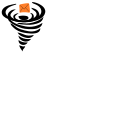
\includegraphics[height=1.1\fontcharht\font`V]{../../../../website/src/main/jbake/assets/images/MessageVortexLogo}}
\gdef\MessageVortex{\texorpdfstring{\emph{MessageVortex}}{MessageVortex}}
\gdef\VortexMessage{\emph{\defref{VortexMessage}}}
\gdef\VortexMessages{\texorpdfstring{\emph{\defref{VortexMessage}s}}{VortexMessages}}
\gdef\VortexNode{\emph{\defref{VortexNode}}}
\gdef\VortexNodes{\emph{\defref{VortexNode}s}}

% quoted environment
\usepackage{libertine}
\newcommand*\quotefont{\fontfamily{LinuxLibertineT-LF}}
\usepackage{etoolbox}
\usepackage{framed}
\newcommand*\quotesize{60} % if quote size changes, need a way to make shifts relative
% Make commands for the quotes
\newcommand*{\openquote}
{\tikz[remember picture,overlay,xshift=-4ex,yshift=-2.5ex]
	\node (OQ) {\quotefont\fontsize{\quotesize}{\quotesize}\selectfont``};\kern0pt}
\newcommand*{\closequote}[1]
{\tikz[remember picture,overlay,xshift=4ex,yshift={#1}]
	\node (CQ) {\quotefont\fontsize{\quotesize}{\quotesize}\selectfont''};}
% select a colour for the shading
\colorlet{shadecolor}{Azure}
\newcommand*\shadedauthorformat{\emph} % define format for the author argument
% Now a command to allow left, right and centre alignment of the author
\newcommand*\authoralign[1]{%
\if#1l
\def\authorfill{}\def\quotefill{\hfill}
\else
\if#1r
\def\authorfill{\hfill}\def\quotefill{}
\else
\if#1c
\gdef\authorfill{\hfill}\def\quotefill{\hfill}
\else\typeout{Invalid option}
\fi
\fi
\fi}
% wrap everything in its own environment which takes one argument (author) and one optional argument
% specifying the alignment [l, r or c]
%
\newenvironment{shadequote}[2][l]%
{\authoralign{#1}%
\ifblank{#2}%
{\def\shadequoteauthor{}\def\yshift{-2ex}\def\quotefill{\hfill}}%
{\def\shadequoteauthor{\par\authorfill\shadedauthorformat{#2}}\def\yshift{2ex}}%
\begin{snugshade}\begin{quote}\openquote}%
{\shadequoteauthor\quotefill\closequote{\yshift}\end{quote}\end{snugshade}}

% Allow byte field graphs
\usepackage{bytefield}


% Allow unbreakable hyphens
\usepackage[shortcuts]{extdash}

% set numbering for subsubsections
\setcounter{secnumdepth}{3}
\setcounter{tocdepth}{2}

% highlighting
\usepackage[bordercolor=white,backgroundcolor=gray!30,linecolor=black,colorinlistoftodos]{todonotes}
\newcommand{\hilight}[1]{\colorbox{yellow}{#1}}

% allow clever references
\usepackage{cleveref}

\gdef\shadowshift{-3pt}
\definecolor{operationcolor}{RGB}{255,226,226}
\definecolor{endoperationcolor}{RGB}{255,255,226}
\definecolor{atomicopcolor}{RGB}{217,248,217}
\definecolor{senderkeycolor}{RGB}{159, 216, 255 }
\definecolor{payloadcolor}{RGB}{233,45,64}
\definecolor{peerkeycolor}{RGB}{217,248, 217}
\definecolor{hostkeycolor}{RGB}{190,217, 232}
\definecolor{layercolor}{RGB}{190,217, 232}
\definecolor{nodecolor}{RGB}{132, 151, 176}
\definecolor{startnodecolor}{RGB}{192, 151, 176}
\definecolor{endnodecolor}{RGB}{132, 211, 176}
\definecolor{nodeshadow}{RGB}{107, 107, 107}
\definecolor{hostIdentitycolor}{RGB}{255, 226, 226 }
\definecolor{transportcolor}{RGB}{220,20,20}
\definecolor{flowColor}{RGB}{ 79,136, 187}
\definecolor{flowBorderColor}{RGB}{ 79,116, 167}
\definecolor{unrelatedcolor}{RGB}{20,220,20}

\graphicspath{{./}{inc/}{../../../../website/src/main/jbake/assets/images/}{../../../../../website/src/main/jbake/assets/images/}}


\begin{document}%
%
\frontmatter%
%\newgeometry{margin=0.1cm, footskip=1mm}
\begin{titlepage}
\makeatletter
\ifdraft
	\begin{tikzpicture}[remember picture,overlay]
	  \node[rotate=60,scale=10,text opacity=0.8] at (current page.center){\color{red}\textbf{\Huge DRAFT}};
	\end{tikzpicture}
\else	
\fi
\makeatother
\pagecolor{gray}\afterpage{\nopagecolor}
\begin{center}~\\[-2.5cm]
\includegraphics[height=0.3\paperwidth]{../../../../website/src/main/jbake/assets/images/MessageVortexLogo_huge}~\\[1cm]

% Title
\newcommand{\HRule}{\rule{\linewidth}{0.5mm}}
\HRule \\[0.4cm]
{ \huge \bfseries \makeatletter\@title\par\normalsize\@subtitle\makeatother \\[0.4cm] }

\HRule \\[3.0cm]

{\large Inauguraldissertation}\\
zur\\
Erlangung der Würde eines Doktors der Philosophie\\
vorgelegt der\\
Philosophisch-Naturwissenschaftlichen Fakultät\\
der Universität Basel\\
von\\
Martin Gwerder (06-073-787)\\
von Glarus GL\\

\vfill
% Bottom of the page
{\large \the\year \\[1cm]}
{\footnotesize Original document available on the edoc sever of the university of Basel edoc.unibas.ch.\\[0.5cm]

\includegraphics[height=7mm]{./inc/cclic.png}~\\[0.5cm]
This work is published under  "Creative Commons Attribution-NonCommercial-NoDerivatives 3.0 Switzerland" (CC BY-NC-ND 3.0 CH) licensed. The full license can be found at \url{http://creativecommons.org/licenses/by-nc-nd/3.0/ch/}.
}

\end{center}
\end{titlepage}

%\restoregeometry
\onecolumn
\clearpage\pagestyle{plain}

\begin{center}

Genehmigt von der Philosophisch-Naturwissenschaftlichen Fakult\"at\\
Auf Antrag von\\[0.5cm]
Prof. Dr. Christian F. Tschudin und Prof. Dr. Ulrich Ultes-Nitsche\\[0.5cm]

Basel, der 25.5.2021 durch die Fakultätsversammlung\\[2cm]
{\rule{6cm}{0.2pt}\\ Prof. Dr. Martin Spiess}
\end{center}
\clearpage



\section*{\abstractname}   
\myabstract

\vspace*{\fill}

\section*{Acknowledgments}
I want to thank my wife, Cornelia, and my lovely three kids, Saphira, Florian, and Aurelius, for their patience and support. Without them, I could never have done this work.

I want to thank Prof. Dr. C. Tschudin and the University of Basel for the possibility of writing this work and for the challenges they opposed to me, allowing me to grow. 

Dr. Andreas Hueni was very supportive by challenging my work with his outside-the-normal-box thinking.

Prof. Dr. Carlos Nicolas of the University of Northwestern Switzerland for being such a valuable sparring partner allowing me to test my ideas.

I want to acknowledge all the individuals who have coded for the \LaTeX{} project for free. Due to their efforts, we can generate professionally typeset PDFs (and far more) for free.

%\fxwarning{unify receiver and recipients}
%\fxwarning{Add co-referent to the list}
%\fxwarning{add lectorer}






%!TeX program=pdflatex
%!TeX encoding=utf8
%!TeX spellcheck = en_US
%!TeX root = ../../messageVortex.tex

\cleardoublepage
\makeatletter
\renewcommand{\@pnumwidth}{4em}
\renewcommand*\l@section{\@dottedtocline{1}{1.5em}{3em}}
\renewcommand*\l@subsection{\@dottedtocline{2}{3.8em}{3.8em}}
\renewcommand*\l@subsubsection{\@dottedtocline{3}{7.4em}{5em}}
% Special Part
\renewcommand*\l@part[2]{%
	\ifnum \c@tocdepth >-2\relax
	\addpenalty{-\@highpenalty}%
	\addvspace{2.25em \@plus\p@}%
	\setlength\@tempdima{3em}%
	\begingroup
	\parindent \z@ \rightskip \@pnumwidth
	\parfillskip -\@pnumwidth
	\begin{tcolorbox}[colback=head, right=0ex, left=0cm, sharpish corners, boxrule=0mm, width=1.0\textwidth]
		{\leavevmode
			\large \bfseries \vbox{\color{white}\sffamily\bfseries#1}%
			\hb@xt@0ex{\color{white}\hss #2}
		}
	\end{tcolorbox}
	\vspace*{1ex}
	\nobreak
	\global\@nobreaktrue
	\everypar{\global\@nobreakfalse\everypar{}}%
	\endgroup
	\fi}
\makeatother

\pagestyle{scrheadings}

\onecolumn
%\setpnumwidth{2em}
%\setlength\cftsectionnumwidth{3em}
\setcounter{tocdepth}{4}
\tableofcontents

\newpage
\indexes
%\twocolumn

\makeatletter
\newlength\mylena
\newlength\mylenb
\setlength\mylena{1.3cm}
\setlength\mylenb{\dimexpr\columnwidth-\mylena\relax}

\newcommand\PlaceNumber[1]{%
	\makebox[\mylena][l]{#1}}

\titleformat{\chapter}
{\Large\sffamily\bfseries}
{}
{0em}
{\PlaceNumber{\thechapter}\parbox[t]{\mylenb}{\raggedright#1}}

\titlespacing*{\chapter}{0pc}{3ex \@plus4pt \@minus3pt}{5pt}

\titleclass{\chapter}{straight}%% added
\makeatother



\mainmatter
\startcontents
%!TeX program=pdflatex
%!TeX encoding=utf8
%!TeX spellcheck = en_US
%!TeX root = ../../messageVortex.tex

\part{Introduction}
\chapter{Foreword}
Almon Brown Strowger was the owner of a funeral parlor in St. Petersburg. He filed a patent on March \nth{10}, 1891 for an ``Automatic Telephone Exchange'' \cite{pulseDialingPatent}. This patent built the base for modern automated telephone systems. According to several sources, he was annoyed by the fact that the local telephone operator was married to another undertaker. She diverted potential customers of Mr. Strowger to her husband instead, which caused Almon B. Strowger to lose business. In 1922, this telephone dialing system, which is nowadays called pulse dialing, became the standard dialing technology for more than 70 years until tone dialing replaced it.

This dialing technology is the base for automatic messaging for voice and text messages (e.g., telex) up until today and is the foundation for current routed networks. These networks build the base for our communication-based Society these days and allow us to connect quickly with any person or company of our wish. We use these networks today as communication meaning for all purposes, and most of the people spend minimal thoughts on the possible consequences arising if someone puts hands on this communication. 

This collected data may be used to judge our intentions and thus is not only confidential if we have something to hide. This problem has dramatically increased in the last years as big companies and countries started to collect all kinds of data and created the means to process them. It allows supposedly to judge peoples not only on what they are doing but as well, on what they did and what they might do. Numerous events past and present show that actors, some of which are state-sponsored, collected data on a broad base within the Internet. Whether this is a problem or not is a disputable fact. Undisputed is, however, that such data requires careful handling, and accusations should then base on solid facts. While people may classify personalized advertising as legit use, a general classification of citizens is broadly considered unacceptable\cite{NCR2013,XKeyscore,Ball2013,Greenberg2013,Leuenberger1989}.

To show that this may happen even in democracies, we might refer to events such as the ``secret files scandal'' (or  ``Fichenskandal'') in Switzerland. In the years from 1900 to 1990 Swiss government collected 900’000 files in a secret archive (covering more than 10\% of the natural and juristic entities within Switzerland at that time). The Swiss Federal Archives document this event in depth\cite{Leuenberger1989}.

Whistleblower Edward Snowden leaked a vast amount of documents. These documents suggest that such attacks on privacy are commonly made on a global scale. The documents leaked in 2009 by him claim that there was a data collection starting in 2010. Since these documents are not publicly available, it is hard proving the claims based on these documents. However -- A significant number of journalists from multiple countries screened these documents claiming that the information seems credible. According to these documents (verified by \href{http://www.nrc.nl/nieuws/2013/11/23/nederland-sinds-1946-doelwit-van-nsa}{NRC}), NSA infiltrated more than 50k computers with malware to collect classified or personal information. They furthermore infiltrated Telecom-Operators (mainly executed by British GCHQ) such as Belgacom to collect data and targeted high members of governments even in associated states (such as the mobile phone number of Germany's president) \cite{NCR2013,XKeyscore,Ball2013,Ackerman2013,Greenberg2013}. A later published shortened list of ``selectors'' in Germany showed 68 telephone and fax numbers targeting economy, finance, and agricultural parts of the German government. A global survey done by the freedom house\cite{FOTN2018} claims a decrease in Internet freedom for the \th{8} year in a row. 

This list of events shows that big players are collecting and storing vast amounts of data for analysis or possible future use. The list of events also shows that the use of such data was at least partially questionable. This work analyses the possibility of using state-of-the-art technology to minimize the information footprint of a person on the Internet. 

We leave a large information footprint in our daily communication. On a regular email, we disclose everything in an ``postcard'' to any entity on its way. Even when encrypting a message perfectly with today's technology (S/MIME\cite{RFC2045} or PGP\cite{RFC2015}), it still leaves at least the originating and the receiving entity disclosed, or we rely on the promises of a third party provider which offers a proprietary solution. Even in those cases, we leak pieces of information such as ``message subject'', ``frequency of exchanged messages'', ``size of messages'', or ``client being used''. A suitable anonymity protocol must cover more than the sent message itself. It includes, besides the message itself, all metadata, and all the traffic flows. Furthermore, a protocol to anonymize messages should not rely on the trust of infrastructure other than the infrastructure under control of the sending or receiving entity. Trust in any third party might be misleading in terms of security or privacy.

Furthermore, central infrastructure is bound to be of particular interest to anyone gathering data. Such control by an adversary would allow manipulating the system or the data or the data flow. So, avoiding a central infrastructure is a good thing when it comes to minimizing an information footprint available to a single entity.

Leaving no information trail when sending information from one person to another is hard to achieve. Most messaging systems disclose at least the peer partners when posting messages. Metadata such as starting and endpoints, frequency, or message size are leaked in all standard protocols even when encrypting messages.

Allowing an entity to collect data may affect senders and recipients of any information. The collection of vast amounts of data allows a potent adversary to build a  profile of a person. Unlike in the past, the availability of information has risen to a never known extent with the Internet.

An entity in possession of such Profiles may use them for many purposes. These include service adoption, directed advertising, or classification of citizens. The examples given above show that the effects of this data is not limited to the Internet but reaches us effectively in the real world.

The main problem of this data is that it may be collected over a considerable amount of time and evaluated at any time. It even happened that standard practices at a time are differently judged upon at a later time. Persons may then be judged retrospectively upon these types of practice. This questionable type of judgment is visible in the tax avoidance discussion\cite{Amat1999}. 

People must be able to control their data footprint. Not providing these means does effectively allow any country or a more prominent player to ban and control any number of persons within or outside the Internet. 

We design in this work a new protocol. This protocol allows message transfer through existing communication channels. These messages are next to unobservable to any third party. This unobservability does not only cover the message itself but all metadata and flows associated with it. We called this protocol ``\emph{MessageVortex}'' or just ``\emph{Vortex}''. The protocol is capable of using a wide variety of transport protocols. It is even possible to switch protocols while the messages are in the transfer. This behavior allows media breaches (at least on a protocol level) and makes the analysis even harder.

The new protocol allows secure communication without the need to trust the underlying transport media. Furthermore, the usage of the protocol itself is possible without altering the immediate behavior of the transport layer. The transport layers' regular traffic does, therefore, increase the noise in which hidden information has to be searched. 

This work splits into multiple parts. In the first part, we collect available researches and technologies. We emphasize techniques on the strength and weaknesses relevant to this work. 

In the second part, we reassemble the pieces to a new protocol. 

In the third part, we analyze the protocol for the fitness of the purpose. We try to find weaknesses and work out recommendations for protocol usage. 

In the last part, we discuss the results and try to summarize the findings. We furthermore elaborate to what extent the protocol fulfills the requirements mentioned in the previous sections.

\section{Contributions}
This thesis contributes to the topic in the following senses:
\begin{itemize}
	\item It introduces a consistent model for message delivery, which includes all endpoints and involved parties.
	\item It shows an approach based on existing protocols for anonymous communication, which gives full control of the anonymity to the sender while controlling the costs.
	\item It offers a client application implementing the proposed Protocol as IMAPv4 cache daemon and as SMTP relay.
\end{itemize}

\chapter{Notation}
\section{Cryptography \label{sec:encNot}}
The theory in this document is heavily based on symmetric encryption, asymmetric encryption, and hashing. To use a uniformed notation I use $E^{K_a}(M)$ (where $a$ is an index to distinguish multiple keys) resulting in $\mathbf{M^{K_a}}$ as the encrypted message. If we are reflecting a tuple of information, we write it in boldface. To express the content of the tuple, we use angular brackets $\mathbf{L\langle normalAddress,vortexAddress\rangle }$. If we want Messages encrypted with multiple keys do list the used keys as a comma-separated list in superscript $E^{K_b}\left(E^{K_a}\left(M\right)\right)=M^{{K_{a}},{K_b}}$.

For a symmetric encryption of a message $\mathbf{M}$ with a key $K_a$ resulting in $\mathbf{M^{K_a}}$ where $a$ is an index to distinguish different keys. Decryption uses therefore $D^{K_a}(\mathbf{M^{K_a}})=\mathbf{M}$.

As notation for asymetric encryption we use $E^{K^{1}_a}(\mathbf{M})$ where as $K^{-1}_a$ is the private key and $K^{1}_a$ is the public key of a key pair $K^p_a$. The asymmetric decryption is noted as $D^{K^{-1}_a}(\mathbf{M})$.

For hashing, we do use $H(\mathbf{M})$ if unsalted and $H^{S_a}$ if using a salted hash with salt $S_a$. The generated hash is shown as $H_M$ if unsalted and $H^{S_a}_M$ if salted.

If we want to express what details contained in a tuple we use the the notation $\mathbf{M\langle t,MURB,serial\rangle }$ respectively if encrypted $\mathbf{M^{K_{a}}\langle t,MURB,serial\rangle}$.

\begin{align*}
\text{asymetric:}         & E^{K^{-1}_a}\left(\mathbf{M}\right)                            && =\mathbf{M}^{K^{-1}_a}\\
& D^{K^{1}_a}\left(E^{K^{-1}_a}\left(\mathbf{M}\right)\right)    && =\mathbf{M}\\
& D^{K^{-1}_a}\left(E^{K^{1}_a}\left(\mathbf{M}\right)\right)    && =\mathbf{M}\\
\text{symetric:}          & E^{K_a}\left(\mathbf{M}\right)                                 && =\mathbf{M}^{K_a}\\
& D^{K_a}\left(E^{K_a}\left(\mathbf{M}\right)\right)          && =\mathbf{M}\\
\text{hashing (unsalted):}& H\left(\mathbf{M}\right)                                       && =\mathbf{H}_M\\
\text{hashing (salted):}  & H^{S_a}\left(\mathbf{M}\right)                                 && =\mathbf{H}^{S_a}_M
\end{align*}

In general, subscripts denote selectors to differentiate the values of the same type, and superscript denotes relevant parameters to operations expressed. The subscripted and superscripted pieces of information are omitted if not needed.

We refer to the components of a \emph{VortexMessage} as follows:
\begin{align*}
\text{Prefix component:}         & \mathbf{PREFIX}                 &=D^{K^{1}_a}\left(\mathbf{P}^{K^{-1}_a}\right) &=D\left(\mathbf{P}\right)\\
\text{Header component:}         & \mathbf{HEAD}                 &=D^{K^{1}_a}\left(\mathbf{H}^{K^{-1}_a}\right) &=D\left(\mathbf{H}\right)\\
\text{Route component:}         & \mathbf{ROUTE}                 &=D^{K^{1}_a}\left(\mathbf{R}^{K^{-1}_a}\right) &=D\left(\mathbf{R}\right)\\
\end{align*}

In general, a decrypted Block is written as a capitalized multi-character boldface sequence. An encrypted Block is expressed as a capitalized, single character, boldface letter.

\section{Code and commands}
We write code blocks as a light grey block with line numbers:

\begin{lstlisting}
public class Hello {
public static void main(String args[]) {
System.println("Hello. "+args[1]);
}
}
\end{lstlisting}

Commands entered at the command line are in a grey box with a top and bottom line. Whenever root rights are required, the command line is prefixed with a ``\#''. Commands not requiring specific rights are prefixed with a ``\$''. Lines without a trailing ``\$'' or ``\#'' are output lines of the previous command. If long lines are split to fit into the paper, a ``$\hookleftarrow$'' is inserted to indicate that a line break was inserted for readability.

\begin{lstlisting}[language=bash]
# su -
# javac Hello.java 
# exit
$ java Hello
Hello.
$ java Hello "This is a very long command-line that had to be broken to fit into the code box displayed on this page."
Hello. This is a very long command-line that had to be broken to fit into the code box displayed on this page.
\end{lstlisting}

\section{Hyperlinking}
The electronic version of this document is hyperlinked. References to the glossary or the literature may be clicked to find the respective entry. Chapter or table references are clickable too. 


%!TeX program=pdflatex
%!TeX encoding=utf8
%!TeX spellcheck = en_US
%!TeX root = ../../messageVortex.tex

% ********************************************************************************************************
% *** Intro to MessageVortex
% ********************************************************************************************************
% ********************************************************************************************************
% *** Research Preexisting work
% ********************************************************************************************************

\partepigraph{Where does a snake's tail start?}{My son Florian}
\DeclareFixedFootnote{\omitted}{footnotes omitted in quote}
\part{Relevant Concepts and Technologies}
\fxwarning{complete section}

\chapter{Anonymity Research}
In this section, we collect protocols research related to anonymity. We did not stick to anonymous message transfer. Instead, we took a broad focus in terms of technology and outlined in each protocol strengths and weaknesses identified, which may be relevant to this research.

\section{Definition of Anonymity}
As the definition for Anonymity we take the definition as specified in \cite{anonTerminology}.
\begin{quote}
	Anonymity of a subject means that the subject is not identifiable within a set of subjects, the anonymity set.\omitted
\end{quote}
and
\begin{quote}
	Anonymity of a subject from an attacker's perspective means that the attacker cannot sufficiently identify the subject within a set of subjects, the anonymity set.\omitted
\end{quote}

We define the anonymity set as the set of all possible subjects within a supposed message. The anonymity of a subject towards an observing third party is a crucial factor as it relates directly to our adversary model.

\section{\texorpdfstring{$k$}{k}-Anonymity}
$k$-anonymity is a term introduced in \cite{k-anonymous:ccs2003}. This work claims that entities are not responsible for an action if an observer is unable to match a specific action to less than $k$ entities.

The Document distinguishes between \textit{Sender $k$-anonymity}, where the sending entity can only be narrowed down to a set of $k$ entities and \textit{Receiver $k$-anonymity}. 

The size of $k$ is a crucial factor. One of the criteria is the legal requirements of the jurisdiction. Depending on the jurisdiction, it usually is not possible to prosecute someone if an action is not directly coupled to one person. Another criterion might be the decreasing of $k$ over time. If a Vortex account is used, we have to assume that some vortex identities go out of commission over time. If $k$ is chosen according to a legal requirement, it should be taken into account that $k$ might be decreasing over time.

\section{\texorpdfstring{$\ell$}{l}-Diversity}
In \cite{machanavajjhala2007diversity} an extended model of $k$-anonymity is introduced. In this paper, the authors emphasize that it is possible to break a $k$-anonymity set if there is additional information available which may be merged into a data set so that a distinct entity can be filtered from the $k$-anonymity set. In other words, if an anonymity set is to tightly specified, additional background information might be sufficient to identify a specific entity in an anonymity set.

It might be arguable that a $k$-anonymity in which a member is not implicitly $k$-anonymous still is sufficient for $k$-anonymity in its sense. However, the point made in this work is right and is taken into account. Their approach is to introduce an amount of invisible diversity into $k$-anonymous sets, so that common background knowledge is no longer sufficient to isolate a single member.

\section{\texorpdfstring{$t$}{t}-Closeness}
While $\ell$-diversity protects the identity of an entity, it does not prevent information gain. A subject which is in a class has the same attributes. This is where $t$-closeness\cite{li2007t} comes into play. $t$-closeness is defined as follows:

\begin{quote}
	An equivalence class is said to have $t$-closeness if the distance between the distribution of a sensitive attribute in this class and the distribution of the attribute in the whole table is no more than a threshold. A table is said to have $t$-closeness if all equivalence classes have $t$-closeness.
\end{quote}

\section{Single Use Reply Blocks and Multi-Use Reply Blocks}
Chaum first introduced the use of reply blocks in \cite{CHAUM1}. A routing block, in general, is a structure allowing to send a message to someone without knowing the targets' real address. Reply blocks may be differentiated into two classes ``Single Use Reply Blocks'' (SURBs)  and ``Multi-Use Reply Blocks'' (MURBs). SURBs may be used once while MURBs may be used a limited number of times. 

Within our research, we discovered that if a routing protocol is reproducible, the traffic of a MURB may be used to identify some of the properties of the message. Depending on the type of attack, the block has to be repeated very often. For this reason, we limited the number of replays to a low number. The concept is that we have, in our case a routing block, which might be used up to $n$ times ($0<n<127$). It is easily representable in a byte integer (signed or unsigned) on any system. It is big enough to support human communication sensibly and is big enough to add not too much overhead when rerequesting more MURBs. The number should not be too big because if a MURB is reused, the same pattern of traffic is generated, thus making the system susceptible to statistical attacks.

\section{Censorship}
As a definition for censorship we take
\begin{quote}
	Censorship: the cyclical suppression, banning, expurgation, or editing by an individual, institution, group or government that enforce or influence its decision against members of the public -- of any written or pictorial materials which that individual, institution, group or government deems obscene and ``utterly without redeeming social value,'' as determined by ``contemporary community standards.''
\end{quote}

The definition is attributed to Chuck Stone Professor at the School of Journalism and Mass Communication, University of North Carolina. Please note that ``Self Censorship'' (not expressing something in fear of consequences) is a form of censorship too.

In our more technical we reduce the definition to
\begin{quote}
	Censorship: A systematic suppression, modification, or banning of data in a network by either removal, or modification of the data, or systematic influencing of entities involved in the processing (e.g., by creating, routing, storing, or reading) of this data.
\end{quote}
This simplified definition narrows down the location to the Internet as it is the only relevant location for us.  Furthermore, it limits the definition to the maximum reach within that system.

\subsection{Censorship Resistant}
A censorship-resistant system is a system that allows the entities of the system and the data itself to be unaffected from censorship. Please note that this does not deny the presence of censorship per se. It still exists outside the system. However, it has some consequences for the system itself.

\begin{itemize}
	\item The system must be either undetectable or out of reach for an entity censoring.\\
	The possibility of identifying a protocol or data allows a censoring entity to suppress the use of the protocol itself. 
	\item The entities involved in a system must be untraceable.\\
	Traceable entities would result in a mean of suppressing real-world entities participating in the system.
\end{itemize}

\subsection{Parrot Circumvention}
In \cite{oakland2013-parrot} \citeauthor{oakland2013-parrot} express that it is easy for a human to determine decoy traffic as the content is easily identifiable as generated content. While this is true, there is a possibility here to generate ``human-like'' data traffic to a certain extent. As an adversary may not assume that his messages are replied to, the problem does not boil down to a true Turing test. It remains on a ``passive observer Turing test'', enabling the potential nodes to choose their messages. 

In our design, this is the job covered by the blending layer. The blending layer generates these messages. These messages are context-less or remain in the context of previous conversations.


\chapter{Related Cryptographic Theory and Algorithms}

Whenever dealing with obfuscating data and maintaining the integrity of data, cryptography is the first tool in the hand of an implementer. A vast amount of research in this area does already exist. For this work, we focussed on algorithms either very well researched and implemented or research, which seem very valuable when putting this work into place. 

In symmetric encryption in this paper always assumes that
\begin{eqnarray}
D^{K_a}\left(E^{K_a}\left(\mathbf{M}\right)\right) & = & \mathbf{M}
\end{eqnarray} 

For a key $K_b\neq K_a$ this means

\begin{eqnarray}
D^{K_a}\left(E^{K_b}\left(\mathbf{M}\right)\right) & \neq & \mathbf{M}\\
D^{K_b}\left(E^{K_a}\left(\mathbf{M}\right)\right) & \neq & \mathbf{M}
\end{eqnarray} 

The following candidates have been analyzed:
\begin{itemize}
	\item AES\\
	NIST announced AES in \citeyear{standard2001announcing} as a result of a contest. The algorithm works with four operations (subBytes, ShiftRows, mixColumns, and addRoundKey). These operations are repeated depending on the key length 10 to 14 times. 
	
	AES is up until now (2018) unbroken. It has been weakened in the analysis described in \cite{tao2015improving}, which reduces the complexity by roughly one to two bits. 
	
	\item Camellia\\
	The camellia algorithm is described in \cite{rfc3713}. The key sizes are 128, 192, and 256. Camellia is a Feinstel cipher with 18 to 24 rounds depending on the key size. Up until today, no publication claims break this cipher. 
\end{itemize}

For all asymmetric encryption algorithm in this paper, we may assume that\ldots

\begin{eqnarray}
D^{K^{-1}_a}\left(E^{K^{1}_a}\left(\mathbf{M}\right)\right) & = & \mathbf{M}\\
D^{K^{1}_a}\left(E^{K^{-1}_a}\left(\mathbf{M}\right)\right) & = & \mathbf{M}
\end{eqnarray} 

It is important that 
\begin{eqnarray}
D^{K^{-1}_a}\left(E^{K^{-1}_a}\left(\mathbf{M}\right)\right) & \neq & \mathbf{M}\\
D^{K^{1}_a}\left(E^{K^{1}_a}\left(\mathbf{M}\right)\right)   & \neq & \mathbf{M}
\end{eqnarray} 

And for any other Keypair $K^{p}_a \neq K^{p}_b$
\begin{eqnarray}
D^{K^{-1}_b}\left(E^{K^{1}_a}\left(\mathbf{M}\right)\right)  & \neq & \mathbf{M}\\
D^{K^{1}_b}\left(E^{K^{1}_a}\left(\mathbf{M}\right)\right)   & \neq & \mathbf{M}\\
D^{K^{-1}_b}\left(E^{K^{-1}_a}\left(\mathbf{M}\right)\right) & \neq & \mathbf{M}\\
D^{K^{1}_b}\left(E^{K^{-1}_a}\left(\mathbf{M}\right)\right)  & \neq & \mathbf{M}
\end{eqnarray} 

The number of crypto algorithms was higher than the steganography options. When looking for well-researched algorithms basing on different mathematical problems and having well-defined outlines, numbers dropped dramatically again.

\begin{itemize}
	\item RSA\\
	In \citeyear{Rivest:1978:MOD:359340.359342} the authors \citeauthor{Rivest:1978:MOD:359340.359342} published with \cite{Rivest:1978:MOD:359340.359342} a paper which did revolutionize cryptography for years. In their paper, the authors described an encryption method later to be called RSA, which required a key pair ($K_a$) referenced as public ($K^{1}_a$) and private keys ($K^{-1}_a$). The novelty of this system was that anything encrypted with the public key was only decryptable with the private key and vice versa.
	
	RSA is up until the day of writing this paper not publicly know to be broken (unless a too small key size is used). However -- \citeauthor{Shor97polynomial-timealgorithms} described in \citeyear{Shor97polynomial-timealgorithms} an algorithm which should enable quantum computers to break RSA far faster than done with traditional computers. In the section \ref{sec:keySize} we do elaborate these effects further.
	\item ECC\\
	The elliptic curves were independently suggested by \cite{Miller1986} and \cite{Koblitz04guideto} in 1986. Elliptic curve cryptography started to be widely deployed in the public space in 2006. Since then, it seems to compete very well with the well established RSA algorithm. While being similarly well researched ECC, has the advantage of far shorter key sizes for the same grade of security.
	\item McEliece\\
	McEliece was first implemented and then removed again. The key size to gain equivalent security to RSA1024 was $\approx 1MB$. This was impractical and thus discarded again. This was done, although there is up until now no known quantum capable algorithm reducing the key size of McEliece.
	\item NTRU\\
	In \cite{Hoffstein1998} \citeauthor{Hoffstein1998} described the NTRU algorithm. The inclusion of this algorithm was disputed as it is patented in the united states as US7031468. It was included because the company Security Innovation holding the patent, released the NTRU algorithm on March \thanks{28} 2018 into the public domain according to a blog entry on the company website. While NTRU is not as well researched as RSA, it has been around for more than 20 years without being significantly affected by known attacks.
	\item ElGammal\\
	We rejected ElGamal as a cryptosystem to include. It bases on the same mathematical problems for cryptoanalysis as RSA (discreet logarithms) but is not as common as RSA.
\end{itemize}


Homomorphic encryption, as introduced in \cite{feldman1987practical}, was from the beginning a strong candidate to be used within our work. Unfortunately, we did not find a way to apply the core $addRedundancy$ operation in homomorphic encryption. Transforming the original data to the GF space in an efficient way to apply matrices was not doable and thus rejected.

%\cite{Gentry:2009:FHE:1536414.1536440} %FIXME dangling reference

\section{Deniable Encryption and Steganography}

Deniable encryption and steganography have been considered out-of-bounds for this work. The main reason is that the presence of encryption (which is not deniable in both cases) may be sufficient for a censor to block a message. Adding a layer to make sure that encryption or steganography is deniable, does not add valuable properties to our system as the sheer presence of encryption might be sufficient for censorship. 

\section{Key Sizes\label{sec:keySize}}

The question of key sizes is hard to answer as it depends on the current and future possibilities of an adversary, which is again depending on not foreseeable research. We tried to collect a couple of recommendations.

\href{http://www.ecrypt.eu.org/}{Encrypt II (http://www.ecrypt.eu.org/)} recommends currently for a ``foreseeable future'' 256 Bits for symmetric encryption and for asymmetric encryption based on factoring modulus 15424 Bits. Elliptic Curve Cryptography and Hashing should be sufficient if used with at least 512 Bits. If the focus is reduced to the next $\approx$ 20 years, then the key size recommendations are reduced to 128 Bit for symmetric encryption, 3248 Bits for factoring modulus operations, and 256 Bits for elliptic curves and hashing.

According to the equations proposed by \citeauthor{Lenstra04keylength.} in \cite{Lenstra04keylength.} an asymmetric key size of 2644 Bits respectively symmetric key length of 95 Bits, or 190 Bits for elliptic curves and hashing should be sufficient for security up to the year 2048. 

According to \cite{CNSASuite} (superseding well known and often used \cite{nsa-fact-sheet-B}) data classified up to ``top secret'' should be signed with RSA 3072+ or ECDSA P-384.  For symmetric encryption, they recommend AES 256 Bits, for Hashing at least SHA-384 and for Elliptic curves a 384 Bit sized key.

As it might seem not a wise idea to consider the recommendation of a potential state-sponsored adversary and the Formulas proposed by \citeauthor{Lenstra04keylength.} do not explicitly take quantum computers into account, we follow the advice of ENCRYPT II.

Furthermore, taking all recommendations together, it seems that all involved parties assume the most trust in elliptic curves rather than asymmetric encryption based on factoring modulus.

\section{Cipher Mode}
The cipher mode defines how multiple blocks encrypted with the same key are handled. Main characteristics of cipher modes to us are:
\begin{itemize}
	\item Parallelisable\\ 
	Can multiple parts of a plaintext be encrypted simultaneously? This feature is important for multi CPU and multi-core systems as they can handle parallelizable more efficiently by distributing them on multiple CPUs.
	\item Random access in decryption\\
	Random access on decryption allows efficient partial encryption of a ciphertext.
	\item Initialisation vector\\
	An initialization vector has downsides and advantages. On the downsides is the fact that an initialization vector must be shared with the message or before distributing it. It is essential to understand that the initialization vector itself usually is not treated as a secret. It is not part of the key.
	\item Authentication\\
	Authentication guarantees that the deciphered plaintext has been unmodified since encryption. It does not make a statement over the identity of the party encrypting the text. Such an identifying authentication is referred to as signcryption.
\end{itemize}

We evaluated the most common cipher modes for suitability. For \MessageVortex, we focussed on modes that have the properties parallelizable, random access, and do not do authentication. The main focus, besides the characteristics mentioned above, was on the question of whether there is an open implementation available in java, which is reasonably tested.

\begin{itemize}
	\item ECB (Electronic Code Book)\\
	ECB is the most basic mode. Each block of the cleartext is encrypted on its own. This results in a big flaw: blocks containing the same data will always transform to the same ciphertext. This property makes it possible to see some structures of the plain text when looking at the ciphertext. This solution allows the parallelization of encryption, decryption, and random access while decrypting. Due to these flaws, we rejected this mode.
	\item CBC (Cypher Block Chaining)\\  
	CBC extends the encryption by xor'ing an initialization vector into the first block before encrypting. For all subsequent blocks, the ciphertext result of the preceding block is taken as xor input. This solution does not allow parallelization of encryption, but decryption may be paralleled, and random access is possible. As another downside, CBC requires a shared initialization vector. As with most IV bound modes, an IV/key pair should not be used twice, which has implications for our protocol.
	\item PCBC (Propagation Cypher Block Chaining)\\
	CBC extends the encryption by xor'ing, not the ciphertext but a xor result of ciphertext and plaintext. This modification denies parallel decryption and random access compared to CBC.
	\item EAX\\      
	EAX has been broken in 2012\cite{minematsu2013attacks} and is therefore rejected for our use.
	\item CFB (Cypher Feedback)
	CFB is specified in \cite{dworkin2001recommendation} and works precisely as CBC with the difference that the plain text is xor'ed and the initialization vector, or the preceding cipher result is encrypted. CFB does not support parallel encryption as the ciphertext input from the preceding operation is required for an encryption round. CFB does, however, allow parallel decryption and random access.
	\item OFB\\
	\cite{dworkin2001recommendation} specifies OFB and works exactly as CFB except for the fact that not the ciphertext result is taken as feedback but the result of the encryption before xor'ing the plain text. This denies parallel encryption and decryption, as well as random access.
	\item OCB (Offset Codebook Mode)\\
	This mode was first proposed in \cite{rogaway2003ocb} and later specified in \cite{krovetz-ocb-04}. OCB is specifically designed for AES128, AES192, and AES256. It supports authentication tag lengths of 128, 96, or 64 bits for each specified encryption algorithm. OCB hashes the plaintext of a message with a specialized function $H_{OCB}(\mathbf{M})$. OCB is fully parallelizable due to its internal structure. All blocks except the first and the last can be encrypted or decrypted in parallel.
	\item CTR\\
	CTR is specified in \cite{lipmaa2000ctr} and is a mixture between OFB and CBC. A nonce concatenated with a counter incrementing on every block is encrypted and then xor'ed with the plain text. This mode allows parallel decryption and encryption, as well as random access. Reusing IV/Key-pairs using CTR is a problem as we might derive the xor'ed product of two messages. This problem only applies where messages are not uniformly random such as in an already encrypted block.
	\item CCM\\
	Counter with CBC-MAC (CCM) is specified in \cite{rfc3610}. It allows to pad and authenticate encrypted and unencrypted data. It furthermore requires a nonce for its operation. The size of the nonce is dependent on the number of octets in the length field. In the first 16 bytes of the message, the nonce and the message size is stored. For the encryption itself, CTR is used. It shares the same properties as CTR. 
	
	It allows parallel decryption and encryption as well as random access.
	\item GCM (Galois Counter Mode)\\
	GCM has been defined in \cite{mcgrew2004galois}, and is related to CTR but has some major differences. The nonce is not used (just the counter starting with value 1). To authenticate the encryption, an authentication token $auth$ is hashed with $H_{GFmult}$ and then xor'ed with the first cipher block. All subsequent cipher blocks are xor'ed with the previous result and then hashed again with $H_{GFmult}$. After the last block the output $o$ is processed  as follows: $H_{GFmult}(o\bigoplus (len(A)||len(B))) \bigoplus E^{K^0}(counter_0)$. As a result, GCM is not parallelizable and does not support random access.
	
	The mode has been analyzed security-wise in \citeyear{mcgrew2004security} and showed no weaknesses in the analyzed fields \cite{mcgrew2004security}. 
	
	GCM supports parallel Encryption and decryption. Random access is possible. However, authentication of encryption is not parallelizable. The authentication makes it unsuitable for our purposes. Alternatively, we could use a fixed authentication string.
	\item XTS (XEX-based tweaked-codebook mode with ciphertext stealing)\\
	This mode is standardized in IEEE 1619-2007 (soon to be superseded). A rough overview of XTS may be found at \cite{Martin2010}. It was developed initially for Disks offering random access and authentication at the same time. 
	\item CMC (CBC-mask-CBC) and EME (ECB-mask-ECB)\\ 
	In \cite{Halevi:2003} \citeauthor{Halevi:2003} introduces a cipher mode which is extremely costly as it requires two encryptions. CMC is not parallelizable due to the underlying CBC mode, but EME is. 
	\item LRW\\
	LRW is a tweakable narrow-block cipher mode described in \cite{tschorsch:translayeranon}. This mode shares the same properties as EBC but without the weakness of the same clear text block resulting in the same ciphertext. Similarly to XEX, it requires a tweak instead of an IV.
\end{itemize}

\section{Summary of Cipher Modes}

\begin{table}[ht]
	\centering\tiny
	\begin{tabular}{|l|l|l|l|l|}\hline
		\diaghead{\theadfont Mode Criteria}{Mode}{Criteria}         & \thead{auth}  &\thead{Requires IV}               & \thead{parallelisable}     & \thead{random access}\\
		\hline
		CBC                                                            & $\times$        & $\checkmark$                      & $\times$                & $\times$\\                      
		CCM                                                            & $\times$        & $\checkmark$                      & $\times$                   & $\times$\\
		CFB                                                            & $\times$        & $\checkmark$                      & $\checkmark$            & $\checkmark$\\              
		CTR                                                            & $\times$        & $\checkmark$                      & $\checkmark$               & $\checkmark$\\              
		ECB                                                            & $\times$        & $\times$                          & $\checkmark$            & $\checkmark$\\   
		GCM                                                            & $\checkmark$    & $\checkmark$                      & $\times$                   & $\times$\\              
		OCB          & $\checkmark$& $\times$\footnotemark[1]    &$\times$                    &$\times$\\
		OFB          & $\times$    & $\checkmark$                &$\times$                    &$\times$\\
		PCBC         & $\times$    & $\checkmark$                &$\times$                    &$\times$\\
		XTS          & $\times$    & $\checkmark$\footnotemark[2]&$\checkmark$                &$\times$\\
		LRW          & $\times$    & $\checkmark$\footnotemark[2]&$\checkmark$                & $\checkmark$\\
		CMC          & $\times$    & $\checkmark$\footnotemark[2]& $\times$                   & $\times$\\
		EME          & $\times$    & $\checkmark$\footnotemark[2]& $\checkmark$                    & $\checkmark$\\              
		\hline          
	\end{tabular}    
	\caption{comparison of encryption modes in terms of the suitability}
	\label{tab:ModeSuitCrit}
\end{table}
\footnotetext[1]{included in auth}
\footnotetext[2]{Requires tweak instead of IV}

\section{Padding}
A plain text stream may have any length. Since we always encrypt in blocks of a fixed size, we need a mechanism to indicate how many bytes of the last encrypted block may be safely discarded. 

Different paddings are used at the end of a cipher stream to indicate how many bytes belong to the decrypted stream.

\subsubsection{RSAES-PKCS1-v1\_5 and RSAES-OAEP}
This padding is the older of the paddings standardized for PKCS1. It is basically a prefix of two bytes followed by a padding set of non zero bytes and then terminated by a zero byte and then followed by the message. This patting may give a clue if decryption was successful or not. RSAES-OAEP ist the newer of the two padding standards 

\subsubsection{PKCS7} 
This padding is the standard used in many places when applying symmetric encryption up to 256 bits key length. The free bytes in the last cipher block indicate the number of bytes being used. This makes this padding very compact. It requires only 1 Byte of functional data at the end of the block. All other bytes are defined but not needed.

\subsubsection{OAEP with SHA and MGF1 padding} 
This padding is closely related to RSAES-OAEP padding. The hash size is, however, bigger, and thus, the required space for padding is much higher. OAEP with SHA and MGF1 Padding is used in asymmetric encryption only. Due to its size, it is important to note that the payload in the last block shrinks to $keySizeInBits/8-2-MacSize/4$.

In our approach, we have chosen to allow these four paddings. The allowed sha sizes match the allowed mac sizes chosen above. It is important to note that padding costs space at the end of a stream. Since we are always using one block for signing, we have to take care that the chosen signing mac plus the bytes required for padding do not exceed the key size of the asymmetric encryption. While this usually is not a problem for RSA as there are keys 1024+ Bits required, it is an essential problem for ECC algorithms as there are much shorter keys needed to achieve an equivalent strength compared to RSA. 

We have introduced an additional type of padding not related to these paddings. We required for the addRedundancy the following unique properties. Unfortunately, we were unable to find any padding which matched the following properties simultaneously:

\begin{itemize}
	\item Padding must not leak successful decryption\\
	For our addRedundancy operation, we required padding that had no detectable structure as a node should not be able to tell whether a removeRedundancy operation did generate content or decoy. 
	\item Padding of more than one block\\
	Due to the nature of the operation, it is required to be able to pad more than just one block.
\end{itemize}

Details of this padding are described in the section "Add and Remove Redundancy Operations'' in \ref{app:rfcMessageVortexMain}. 

\chapter{Censorship Circumvention}
Several technical ways have been explored to circumvent censorship. All seem to boil down to the following main ideas:
\begin{itemize}
	\item Hide data
	\item Copy or distribute data to a vast amount of places to improve the lifespan of data
	\item Outcurve censorship measurements
\end{itemize}

In the following section, we look at technologies and ideas dealing with these circumvention technologies.

\section{Covert Channel and Channel Exploitations}
The original term of covert channels was defined by \citeauthor{Lampson73anote}\cite{Lampson73anote} as 

\begin{quote}
	not intended for information transfer at all, such as the service program's effect on system load.
\end{quote}

This was defined  in such a way to distinguish the message flow from 

\begin{quote}
	legitimate channels used by the confined service, such as the bill.
\end{quote}

The use of a legitimate channel such as \defref{SMTP} and hide information within this specific channel is not a usage of a covert channel. We refer to this as channel exploitation.

\section{Steganography}

Steganography is an important part when it comes to unlinking information. In \cite{6828087} and \cite{subhedar2014current} we get a very rough overview. As some of the types and algorithms address specific topics of steganography (e.g., some hide from automatic detection and others address a human message stream auditor), we need to choose carefully. In our specific case, the main idea is to hide within the sheer mass of Internet traffic. As a human auditor screening all the messages is a minor thread, we focus on machine-based censorship. Most of the images sent in \defref{SMTP} are jpg images (see table \ref{tab:emailAttachments} on page \pageref{tab:emailAttachments}). We limited our search to algorithms capable of hiding binary data within these files. The number of academically researched options was surprisingly low.

After reviewing the options, we decided to go for F5\cite{f5}. It is a reasonably well-researched algorithm which attracted many researchers. The original F5 implementation had a detectable issue with artifacts\cite{F5broken} caused by the recompression of the image. This issue was caused only due to a problem in the reference implementation, and the researchers have provided a corrected reference implementation without the weakness.

% We use https://github.com/matthewgao/F5-steganography

YASS, as described in \cite{solanki2007yass}, was not considered a candidate. Although less researched, researchers found multiple weakness\-es\cite{kodovsky2010modern,li2009steganalysis}.

%other options : MM3 only good below 5% (unclear ; no implementation found);  PQe or PQt only good below 10% (only matlab)
% other algorithms nsF5 (only matlab)

\section{Timing Channels}

Timing channels are a specialized form of covert channels. In timing channels, the information itself hides not within the data of the channel, but the usage of the channel is in such a way that it is capable of reflecting the data. As we do not have control over the timing of the transport channel, this is not an option for us.

\section{Technical Forms of Censorship}
There are many types of censorship available within technical systems. An in-depth understanding of the possibilities is required in order to understand the means of a censoring adversary.

\subsection{Making Systems Unavailable by Censoring Lookups}
This is one of the cheapest method to create censorship. Lookup systems such as DNS servers are modified in such a way that traffic is no longer deliverable or redirected to a system controlled by the censorer.

Many jurisdictions have implemented such measures a very cheap measure of censorship. It is, however, very easy to outcurve. As soon as a user no longer uses adversary controlled lookup services, this form of censorship is ineffective. In the case of DNS this means either: 

\begin{itemize}
	\item Use a public DNS server worldwide available
	\item Use another protocol to hide the traffic 
	\begin{itemize}
		\item A legit protocol with tunnelling capabilities like SSH to a system outside of the reach of the censoring adversary.
		\item Use a fully blown tunnel such as a VPN.
		\item Piggyback a legit protocol such as DNS-over-HTTPS (DoH)\cite{rfc8484} or DNS-over-XMPP\cite{xep0418}
	\end{itemize}
\end{itemize}

\subsection{Making Systems Unavailable by Disrupting System Traffic}
Disruption of traffic is commonly done with packet filtering devices commonly referred as firewalls. These firewalls may filter any traffic to a given system. There are some considerable downsides to this system from the adversary's point of view.

First, it requires high bandwidth. All traffic of a jurisdiction or target must pass through this filtering device. This is usually doable for a country. 

Secondly, the target must be identifiable on a technical level (e.g., IP address) as content based filtering is only feasible with unencrypted or weakly protected systems. This technical identification is hard as systems may change their addresses dynamically either due to cloud related elasticity or simply due to an incomplete view to a distributed system.

\fxwarning{Explain further the problem for people not so much in cloud and networks}

And lastly, The target may not be split (e.g., partial censoring). Censoring platforms such as Youtube or Gmail which are commonly shared among legit and illegit uses from the censorers point-of-view can not be reasonably split. This due to the fact that only the provider of the service can do selective censoring on the system.

\fxwarning{Explain more and maybe add china as an example}

\subsection{Making Systems Unavailable by Interfering with System Traffic}
\fxwarning{May be done by traffic shaping, content moderation}

\section{Spread Spectrum in Networking Protocols}
\fxwarning{Empty section}

\chapter{Other Related Concepts}
\section{Zero Trust\label{sec:zeroTrust}}
Zero trust is not an acdemically defined concept. In fact it is widely misused by many marketing departments of well known devices and applications related to security. The first citation of the concept was in \cite{kindervag2010no} where \citeauthor{kindervag2010no} introduced this concept.

\citeauthor{kindervag2010no} compares the traditional approach as an M\&M (crunchy shell and soft inner part). And introduces the zero trust principle in three concepts:
\begin{quote}
	\begin{enumerate}
		\item Ensure That All Resources Are Accessed Securely Regardless Of Location
		\item Adopt A Least Privilege Strategy And Strictly Enforce Access Control
		\item Inspect And Log All Traffic
	\end{enumerate}
\end{quote}

This concept applies to security and no to anonymity. We therefore had to adopt this concept not violating anonymity.
	\begin{enumerate}
	\item Ensure that all resources are accessed securely regardless of location\\
		  We make sure that control over the security relevant parameters remain at all time within the originator of a message. Violation of transport security should not be possible by malfunctioning or poorly configured nodes.
	\item Adopt a least privilege strategy and strictly enforce access control\\
	      As design principle this means that information is kept hidden as much as possible within the system. We always assume that an adversary
		  \begin{itemize}
			\item makes some or all information within his reach available to others.
			\item Analyze all information within his reach.
			\item Willingly break protocol rules in order to gain information, disrupt information flows, or other advantages.
		  \end{itemize}		
	\item Inspect and log all traffic
	      
\end{enumerate}



%!TeX program=pdflatex
%!TeX encoding=utf8
%!TeX spellcheck = en_US
%!TeX root = ../../messageVortex.tex

\partepigraph{It was the anonymity. He wanted to be unknown, unpossessed by others' knowledge of him. That was freedom.}{Ling Ma, Severance}
\part{Anonymous Communication Systems}\label{sec:systems}
In \cref{sec:standardProtocols} we search for common Internet protocols suitable for hiding our traffic or accommodating data. In \cref{sec:informationHiding} we focus on technologies employed for problems related to anonymization or information hiding in general and analyze in \cref{sec:implSystems} available systems in this field.

\chapter{Well Known Standard Protocols}\label{sec:standardProtocols}
\hiddensection{SMTP and Related Post Office Protocols (1982)}\label{sec:mailTransport}
Today's mail transport is mostly carried out via \defref{SMTP}\index{SMTP} protocol, as specified in~\cite{rfc5321}. This protocol has proven to be stable and reliable. Most of the messages are passed from an Mail User Agent (\defref{MUA}) to an SMTP relay of a provider. From there, the message is directly sent to the recipient's SMTP server and then to the recipient's server-based storage. At any time the recipient may connect to his server-based storage and may optionally relocate the message to a client-based (local) storage. The delivery from the server storage to the MUA of the recipient may occur by message polling or by message push (whereas a push--pull mechanism usually implements the latter).

To understand the routing of a mail, it is essential that we understand the whole chain starting from a user(-agent) until arriving at the target user (and being read!). To simplify this, we used a consistent model that includes all components (server and clients). The figure \ref{fig:MailAgents} shows all involved parties of a typical mail routing. It is essential to understand that mail routing remains the same regardless of the client. However, the availability of mail at its destination changes drastically depending on the type of client used. Furthermore, the mail flow and control over it may differ on the client and the message processing on the server.

The model has three main players \defref{storage}, \defref{agent}, and \defref{service}. Storages are endpoint facilities storing emails received. Not explicitly shown are temporary storages such as spooler queues or state storages. Agents are simple programs handling a specific job. Agents may be exchangeable by other similar agents. A service is a bundle of agents that is responsible for a specific task or task sets.

\begin{figure}[ht!]
	\centering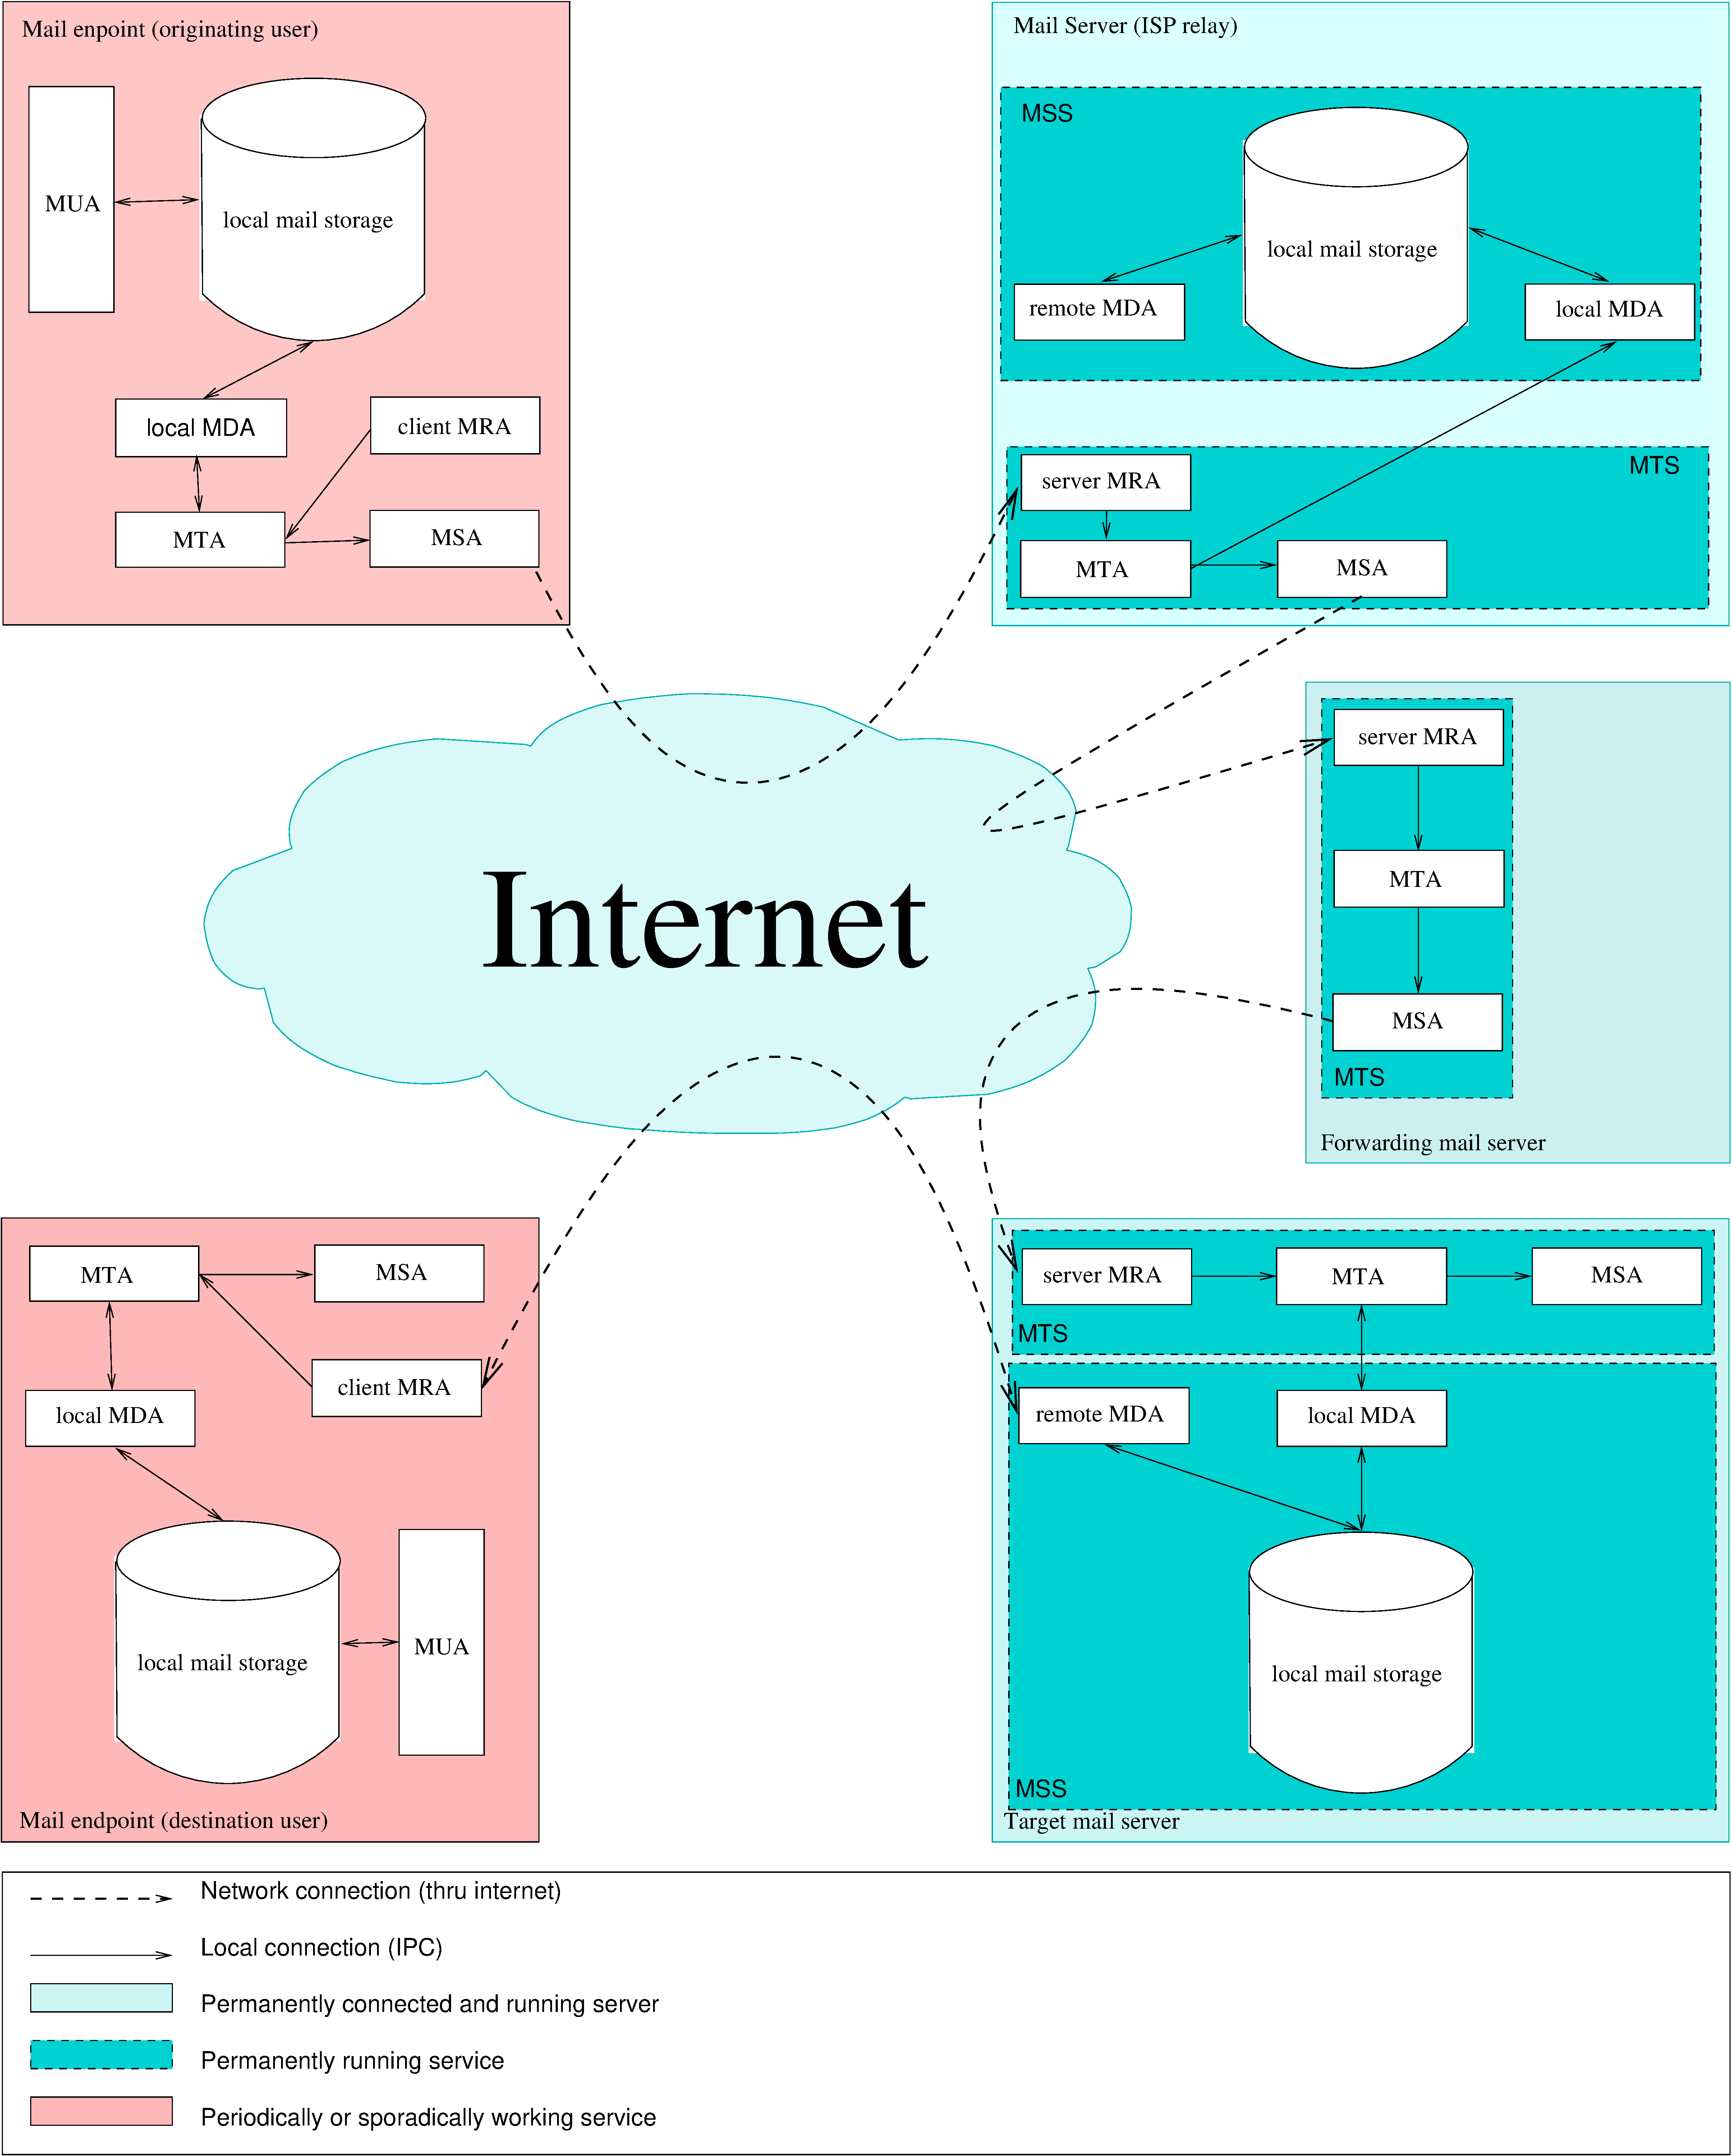
\includegraphics[width=\columnwidth]{inc/MailAgents1.pdf}
	\caption{Mail agents.}
	\label{fig:MailAgents}
\end{figure}

In the following paragraphs (for definitions), the term ``email'' is used synonymously to the term ``Message''.  ``Email'' has been chosen over ``messages'' because of its frequent use in standard documents.

An \defref{MUA}{} accesses local email storage, which may be the server storage or a local copy. The local copy may be a cache only copy, the only existing storage (when emails are fetched and deleted from the server after retrieval), or a collected representation of multiple server storages (cache or authoritative).

In addition to the MUA, the only other component accessing local email storage is the Mail Delivery Agent (\defref{MDA}). An MDA is responsible for storing and fetching emails from the local mail storage. Emails destined for other accounts than the current one are forwarded to the MTA. Emails destined for a user are persistently stored in the local email storage. It is essential to understand that email storage does not necessarily reflect a single mailbox. It may as well represent multiple mailboxes (e.g., a rich client-serving multiple IMAP accounts) or a combined view of multiple accounts (e.g., a rich client collecting mail from multiple \defref{POP} accounts). In the case of a rich client, the local MDA is part of the user agent's software. In the case of an email server, the local MDA is part of the local email store (not necessarily of the mail transport service).

On the server-side, there are usually two components (services) at work. A ``Mail Transport Service'' (\defref{MTS}) responsible for mail transfers, and a ``Mail Storage System'' which offers the possibility to store received mails in a local, persistent store.\par

An MTS generally consists of three parts. For incoming connects, there is a daemon called Mail Receiving Agent (\defref{Server MRA}) is typically a \defref{SMTP} listening daemon. A Mail Transfer Agent (\defref{MTA}) is responsible for routing, forwarding, and rewriting emails. Moreover, a Mail Sending Agent (\defref{MSA}) is accountable for transmitting emails reliably to another server MRA (usually sent via \defref{SMTP}).\par

An MSS consists of local storage and delivery agents, which offer uniform interfaces to access the local store. They also deal with replication issues, and grant should take care of the atomicity of transactions committed to the storage. Typically there are two different kinds of \defref{MDA}s. \defref{Local MDA}s offer possibilities to access the store via efficient (non-network based) mechanisms (e.g., IPC or named sockets). This is usually carried out with a stripped-down protocol (e.g., \defref{LMTP}). For remote agents, there a publicly -- network-based -- agent available. Common Protocols for this \defref{Remote MDA}\ include \defref{POP}, \defref{IMAP}, or \defref{MS-OXCMAPIHTTP}.\par

Mail endpoints consist typically of the following components:
\begin{itemize}
	\item A Mail User agent (\defref{MUA})
	\item A Local Mail storage (\defref{MUA})
	\item A Local Mail Delivery Agent (\defref{Local MDA})
	\item A Mail Transfer Agent (\defref{MTA})
	\item A Mail Sending Agent (\defref{MSA})
	\item A Mail Receiving Agent (\defref{MRA})
\end{itemize}

Only two of these components have external interfaces. These are \defref{MSA} and \defref{MRA}. \defref{MSA} usually uses \defref{SMTP} as transport protocol. This leads to some distinctive features.
\begin{itemize}
	\item Port number is 587 (specified in~\cite{rfc4409}).\\
	Although port numbers 25 and 465 are valid and usually have the same capabilities, they are only for mail routing between servers. Mail endpoints should no longer use them.
	\item Connections are authenticated.\\
	Unlike normal server-to-server (relay or final delivery) SMTP connections on port 25, the server should always authenticate clients of some sort. This may be based on data provided by the user (e.g., username/password or certificate) or data identifying the sending system (e.g., IP address)~\cite{rfc4409}. Failure in completing authentication may result in this port being misused as a sender for \defref{UBM}.
\end{itemize}

Mail User Agents (MUA) are the terminal endpoint of email delivery. Mail user agents may be implemented as fat clients on a desktop or mobile system, or as an interface over a different generic protocol such as HTTP (Web Clients). 

Server-located clients are a special breed of fat clients. They share the properties of fat clients except that they do not connect to the server. The client application itself has to be run on the server where the mail storage persists. This changes delivery and communication with the server. Instead of interfacing with an MSA and a client MDA, they may directly access the server's local mail storage. The local mail storage may be implemented as a database in a user-specific directory structure on these systems.

\hiddensubsection{Fat Clients}
The majority of mail clients are fat clients. They have a locally installed application on the client device to access mail allowing advanced features such as offline reading or bandwidth optimization. These clients score over the more centralistic organized web interfaces (web clients) in that they may offer mail availability even if an Internet connection is not available (through client-specific local mail storage). They furthermore provide the possibility to collect emails from multiple sources and store them in the local storage. Unlike mail servers, clients are assumed not to always be online. They may be offline most of the time. To guarantee the availability of a particular email address, a responsible mail server for a specific address collects all emails (e.g., \defref{MSS}). It provides a consolidated view of the database when a client connects through a local or remote MDA.

As these clients vary heavily, it is mandatory for the MDA that they are well specified. Not doing so would result in massive interoperability problems. Most commonly, the protocols \defref{IMAP}, \defref{POP} and \defref{EWS} are used. For email delivery, the SMTP protocol is used. 

Fat clients are commonly used on mobile devices. According to~\cite{clientDistribution} in August 2012, the most typical fat email client was Apple Mail client on iOS devices ($35.6\%$), followed by Outlook ($20.14\%$), and Apple Mail ($11\%$). \citetitle{clientDistribution2}~\cite{clientDistribution2} as a more recent source lists in February 2014 iOS devices with $37\%$, followed by Outlook ($13\%$), and  Google Android ($9\%$).

\hiddensubsection{Server-Located Clients}
Server-located clients are an absolute minority. This type of client was common in the days of centralized hosts. An example for a server-located client is the Unix command ``mail''. This client reads email storage from a file in the user's home directory.

\hiddensubsection{Web Clients}
Presently, web clients are a common alternative to fat clients. Most large provider companies use their proprietary web client. According to~\cite{clientDistribution2} the most common web clients are "`Gmail"', "`Outlook.com"', and "`Yahoo! Mail"'. All these interfaces do not offer a public plug-in interface. However, they typically do offer IMAP or similar interfaces. This is important for a future, generalistic approach to the problem.

\section{S/MIME (1996)}
S/MIME is an extension of the MIME standard. The MIME standard allows in simple text-oriented mails an alternate representation of the same content (e.g., as text and as HTML) or splitting a message into multiple parts that may be encoded. It is important to note that MIME encoding is only effective in the body part of a mail.

S/MIME, as described in~\cite{rfc3851}, S/MIME extends this standard with the possibility to encrypt mail content or sign it. Practically this is achieved by either putting the encrypted part of the signature into an attachment. It is essential to know that this method leaks significant pieces of the data.

As the mail travels directly from sender to recipient, both involved parties are revealed. Neither the message subject nor the message size or frequency is typically hidden. This method offers limited protection assuming an adversary who is only interested in the messages' content. It does not protect us from the adversary defined in our case. 

The trust model is based on a centralistic approach involving generally trusted root certification authorities.

\section{Pretty Good Privacy (1996)}
Exactly as S/MIME, PGP~\cite{rfc4880} builds on the basis of MIME. Since the trust model in PGP is peer-based, the encryption technology does not significantly differ (as seen from the security model).

Similar to S/MIME, PGP does not offer anonymity. Sender and endpoints are known to all routing nodes. Depending on the version of PGP, some meta information or parts of the message content such as the subject line, the sender and receiver's real name, and the message size are leaked.

An important fact from PGP is that peer-based approaches offer limited possibilities for trust. The trust in PGP is based on the peer review of users. This peer review may give an idea of how well verified the key of a user is.

\section{XMPP}
XMPP (or formerly Jabber) is defined in the RFCs~\cite{rfc6120,rfc6121,rfc3923,rfc3922} and features an own extension process on the base of XEPs. The community is very active in the development and has almost 200 proposed, drafted, active, final, or experimental XEPs. 

At its core, XMPP is an open, secure, decentralized, and extensible standard for real-time capable protocol, allowing the efficient transfer of messages and signal status data. It allows single or multi-user chats and may be used as dialing protocol for voice, video file transfer, and for similar content.

We use XMPP in our work as proof of concept that a switch of protocols (in our case, SMTP and XMPP) is feasible.

The fact that the two protocols significantly differ in their cores makes it an ideal use-case. XMPP is synchronous (whereas SMTP is asynchronous, is not MIME-based (whereas SMTP is)), and has an own implementation for file transfers. On the other hand, it offers many advantages, such as the availability of end-to-end encryption or additional store-and-forward services.


\chapter[Information in Anonymizing Protocols]{Distribution for Anonymizing Protocols and Information Routing}\label{sec:informationHiding}
Information routing and distribution is not a novelty in privacy research. Researchers around the globe have searched for means of privacy. One good example was the patent in the introduction of Almon B. Strowger~\cite{pulseDialingPatent}. More recent activities are the infamous ``How to share a secret''~\cite{shamir1979share}, which used Lagrange polynomials to distribute shares of information across multiple hosts for privacy. A single polynomial would be attackable. Shamir applied a $\mod p$ operation to hide characteristics of a curve (as long as $p$ is large and prime). The system had many problems which were addressed by subsequent work such as~\cite{tompa1989share}.

Lagrange polynomes form an essential part when it comes to networking and privacy. They are commonly used in the form of Reed--Solomon-codes for securing unreliable connections (e.g.,~\cite{aiache2008reed}), distributing data~\cite{shamir1979share}.

Our approach is to use Lagrange not primarily for distributing data but to generate unidentifiable decoy traffic. When applying a Lagrange polynomial to a message, all factors contain parts of the original message. Given enough factors of the polynomial, anyone may reconstruct the original message. As a result, an adversary cannot tell which parts of the traffic are decoy and which part is the message, as all parts can recover the original message.

\section{Mixing}\label{sec:mixNets}
Mixes were first introduced by \citetitle{CHAUM1}~\cite{CHAUM1} in \citeyear{CHAUM1}. The basic concept in a mix is as follows. We do not send a message directly from the source to the target. Instead, we use a proxy server or router in between, which picks up the packet, anonymizes it, and forwards it to the recipient or to another mix. If we assume that we have at least three mixes cascaded, we then can conclude that:
\begin{itemize}
	\item Only the first mix knows the true sender
	\item All intermediate mixes know neither the true sender nor the true recipient (as the data comes from mixes and is forwarded to other mixes) 
	\item Only the final mix knows the final recipient.
\end{itemize}

This approach (in this simple form) has several disadvantages and weaknesses.

\begin{itemize}
	\item In a low latency network, an adversary may trace the message by analyzing the timing of a message.
	\item We can emphasize a path by replaying the same message multiple times (assuming we control an evil node), thus discovering at least the final recipient.
	\item If we can ``tag'' a message (with content or an attribute), we may follow the message.
\end{itemize}

In \citeyear{RP03-1} \citeauthor{RP03-1} analyzed the suitability for mixes as an anonymizing network for masses. They concluded that there are three possibilities to run mixes.
\begin{itemize}
	\item Commercial, static MixNetworks
	\item Static MixNetworks operated by volunteers
	\item Dynamic MixNetworks
\end{itemize}
They concluded that in an ideal implementation, a dynamic mix network where every user operates one mix is the most promising solution as static mixes always might be hunted by an adversary.

\section{Anonymous Remailers}\label{sec:remailers}
Remailers have been in use for quite some time. There are several classes of remailers, and all of them are somehow related to Mix Networks. There are ``types'' of remailers defined. Although these ``types'' offer some hierarchy, none of the more advanced ``types'' seem to have more than one implementation in the wild. 

Pseudonymous remailers (also called Nym Servers) take a message and replace all information pointing to the original sender with a pseudonym. This pseudonym may be used as a reply address. The most well known pseudonymous remailer possibly was anon.penet.fi run by Johan Helsingius. Several times, this service was forced to reveal a pseudonym's true identity before Johan Helsingius decided to shut it down. For a more in-depth discussion of pseudonymous remailers, see \ref{sec:remPseudo}

Cypherpunk remailers forward messages like pseudonymous remailers. Unlike pseudonymous remailers, Cypherpunk remailers decrypt a received message, and its content is forwarded without adding a pseudonym. A reply to such a message is not possible. They may, therefore, be regarded as a ``decrypting reflector'' or a ``decrypting mix'' and may be used to build an onion routing network for messages. For a more in-depth discussion of type-1-remailers, see section  \ref{sec:remCypherpunk}.

Mixmaster remailers are very similar to Cypherpunk remailers. Unlike them, Mixmaster remailers hide the messages, not in an own protocol, but use \defref{SMTP} instead. While using \defref{SMTP} as a transport layer, Cypherpunk remailers are custom (non-traditional) mail servers listening on port 25. For a more in-depth discussion of type-2-remailers, see section \ref{sec:remMixmaster}.

Mixminion remailers extend the model of Mixmaster remailers. They still use \defref{SMTP} but introduce new concepts. New concepts in Mixminion remailers are:
\begin{itemize}
	\item Single Use Reply Blocks (SURBs)
	\item Replay prevention
	\item Key rotation
	\item Exit poicies
	\item Dummy traffic
\end{itemize}
For a more in-depth discussion of Mixminion remailers see section \ref{sec:remMixminion}.


\section{Onion Routing}
Onion routing is a further development of the concept of mixes. In onion routers, every mix receives a message which is asymmetrically encrypted. By decrypting the message, the next hop's name and the content to be forwarded can be obtained. The main difference in this approach is that the mix decides about the next hop in traditional mix cascades. In an onionized routing system, the message chooses the route. 

Onionized messages typically have the problem of a constant size loss throughout the system. Some systems counter this effect by separating the routing setup from the message path.

While tagging attacks are far more demanding (if we exclude side-channel attacks to break sender anonymity), the traditional attacks on mixes are still possible. Thus when an adversary is operating entry and exit nodes, it is straightforward for them to match the respective traffic.

One very well known onion routing network is Tor (\href{https://www.torproject.org}{https://www.torproject.org}). For more information about Tor see section \ref{sec:tor}.

\section{Garlic Routing}
Garlic routing is an improved form of onion routing. It stops onionized messages from continuously loose contents on their way. A garlic router collects multiple, independent messages into one message before routing. This compensates for the ``size loss effect'' of onionized systems.

\section{Crowds}
Crowds is a network that offers anonymity within a local group. It works as follows:

\begin{itemize}
	\item All users add themselves to a group by registering on a so-called ``blender''.
	\item All users start a service (called JonDo).
	\item Every JonDo takes any received message (might be from him as well) and sends it with a 50\% chance either to the correct recipient or to a randomly chosen destination.
\end{itemize}

While crowds, as specified in~\cite{crowds:tissec}, does anonymize the sender from the recipient rather well, the system offers no protection from someone capable of monitoring crowds traffic. The system may, however, be easily attacked from within by introducing collaborating JonDos. It was further developed to D-Crowds~\cite{crowdsAttack}, ADU/RADU~\cite{Munoz-Gea2008}, Freenet~\cite{freenet} and others. 

Furthermore, the blender is aware of all JonDos and thus of particular interest for any observing or censoring adversary. The control of the blender enables an adversary to split the network into controllable parts, adding a high likelihood of discovering the original sender.

\section{Mimic Routes}
Mimics are a set of statical mixes that maintain a constant message flow between the static routes. If legitimate traffic arrives, the pseudo traffic is replaced by legitimate traffic. An outside observer is thus incapable of telling the difference between real traffic and dummy traffic.

If centralized mixes are used, the system lacks the same vulnerabilities of sizing and observing the exit nodes as all previously mentioned systems. If we assume that the sender and receiver operate a mixer themselves, the system would no longer be susceptible to timing or sizing analyses. The mimic routes put a constant load onto the network. This bandwidth is lost and may not be reclaimed. It does not scale well as every new participant increases the need for mimic routes and creates (in the case of user mixes) a new mimic load. Furthermore, the mixes are easily identifiable as their characteristic data stream contrasts with other network service streams.

\section{Distributed Hash Tables}
Anonymous file transfer is quite often based on Distributed Hash Tables (DHTs). Systems like $I^2P$ (see \href{https://geti2p.net/}{geti2p.net}), or Freenet~\cite{freenet} base on DHT. Hash tables are typically used for an efficient lookup of data distributed within a system. As they support the distribution of data, they may implicitly support error tolerance, robustness and, thus, availability. They furthermore may be used as distribution mechanism allowing self-organization, load balancing, and scalability.

In most anonymity systems using DHT, DHTs are either used to cloak the hashed nodes while enabling routing to them, or to build complex anycast structures.

\section{Dining Cryptographer Networks}
DC networks are based on the work \citetitle{chaum-dc} by \citeauthor{chaum-dc}~\cite{chaum-dc}. In this work, \citeauthor{chaum-dc} describes a system allowing a one-bit transfer (the specific paper talks about the payment of a meal). Although all the DC net participants are known, the system makes it unable to determine who sent a message. The message in a DC-net is readable for anyone. This network has the disadvantage that a cheating player may disrupt communication without being traceable.

Several attempts have been made to strengthen the proposal of Chaum~\cite{golle:eurocrypt2004,disco,herbivore:tr,Corrigan-Gibbs:2010:DAA:1866307.1866346}. However, no one succeeded without introducing significant disadvantages on the privacy side.

\section{Private Information Retrieval}
Private Information Retrieval (PIR)~\cite{chor1995private} was developed by \citeauthor{chor1995private}. It is a  public database organized in slots where some clients write into specific slots and other clients access the whole database so that the server is unable to tell what data was accessed. It is a simplified or weaker version of an oblivious transfer (1-out-of-n). PIR was described in theory and had two different approaches. A computationally secured approach (cPIR), which is the weaker one of the two approaches, and the information-theoretic secured approach (itPIR).

PIR was the foundation or an inspiration for many other systems and extensions such as CSPIR~\cite{lipmaa2009first}, BddCpir~\cite{lipmaa2009first}, Popcorn~\cite{gupta2016scalable}, or Riposte~\cite{corrigan2015riposte}.

\chapter[Academic Protocols and Implementations]{Proposed Academic Protocols and Implementations}\label{sec:implSystems}
In this section, we list various proposed anonymity systems regardless of their age or state. We analyze their inner workings and try to compare them in a unified way. This comparison was a basis for selecting our approach.


\section{Characteristics of Known Anonymity Implementations}
Table \ref{tab:anonClass} shows the protocols analyzed in the next sections ordered by type and year according to the classification scheme introduced in~\cite{Shirazi2018}.

\gdef\cc{}
\gdef\cols{
	\ifx\cc\empty
	\gdef\cc{not empty}
	\else
	\gdef\cc{}
	\fi
	\col
}
\gdef\col{%
	\ifx\cc\empty%
	\cellcolor{black!30}%
	\else%
	\cellcolor{black!10}%
	\fi}

\gdef\mybull{\medbullet}
\gdef\mycirc{\medcirc}
\gdef\mytick{\faCheck}
\gdef\mycross{\faTimes}
% network
%\usepackage{ amssymb }
\newcommand\networkFully{$\col\boxtimes$}
\newcommand\networkMostly{\col$\square$}
\newcommand\networkPartly{\col$\sqsubset$}
%direction
\newcommand\directionBidi{\col$\longleftrightarrow$}
\newcommand\directionUnidi{\col$\longrightarrow$}
% synchronization
\newcommand\syncAsync{\col$\neq$}
\newcommand\syncSynchronous{\col$\cong$}
% symmetry
\newcommand\rolePtp{\col\scalebox{0.4}{$\mybull\cdot\cdot\mybull\cdot\cdot\mybull$}}
\newcommand\roleCs{\col\scalebox{0.4}{$\mybull\cdot\cdot\mybull$}}
\newcommand\roleHybrid{\col\scalebox{0.4}{$\mybull\cdot\cdot\mycirc\cdot\cdot\mybull$}}
% Hierarchy
\newcommand\hierarchyFlat{\col$\cdots$}
\newcommand\hierarchyHierarchical{\col\ding{68}}
% centralization
\newcommand\decentralizationPart{\col\astrosun}
\newcommand\decentralizationDecentr{\col$\bigcirc$}
\newcommand\decentralizationNo{\col\mycross}
% Network view
\newcommand\netviewFully{\col$\CIRCLE$}
\newcommand\netviewPartly{\col$\LEFTcircle$}
% NW updating
\newcommand\updatingTimed{\col\clock}
\newcommand\updatingEvent{\col\lightning}
\newcommand\updatingNoupd{\col\mycross}
% Routing
\newcommand\routingRoutesrc{\col\scalebox{0.4}{$\mybull\cdots$}}
\newcommand\routingRoutehop{\col\scalebox{0.4}{$\cdots\mybull\cdots$}}
\newcommand\routingRoutebc{\col\faBullhorn}
% Sheduling
\newcommand\shedfair{\col$\equiv$}
\newcommand\shedprio{\col$\Diamonddot$}
%determinism
\newcommand\nsdetdet{\col\mytick}
\newcommand\nsdetprob{\col\mycross}
%selection set
\newcommand\nsnodesall{\col\CircledA}
\newcommand\nsnodessec{\col\Stopsign}
\newcommand\nsnodesnet{\col\Mundus}
\newcommand\nsnodesusr{\col\smiley}
% probability
\newcommand\nsprobuni{\col$\circledast$}
\newcommand\nsprobstat{\col$\circledcirc$}
\newcommand\nsprobdyn{\col$\ast$}
% latency
\newcommand\perflatl{\col L}
\newcommand\perflath{\col H}
\newcommand\perflatm{\col M}
% mode 
\newcommand\perfmodecon{\col$\multimapdotboth$}
\newcommand\perfmodemsg{\col\Letter}
% implementation
\newcommand\nsimplyes{\col\mytick}
\newcommand\nsimplno{\col\mycross}
% code available
\newcommand\nscodeyes{\col\mytick}
\newcommand\nscodeno{\col\mycross}
% context
\newcommand\nscontmsg{\faEnvelope}
\newcommand\nscontmail{@}
\newcommand\nscontbulletin{\faUsers}
\newcommand\nscontphone{\Telefon}
\newcommand\nscontwww{\faInternetExplorer}
\newcommand\nscontmicroblog\faPencil
\newcommand\nscontfiles\faStickyNote
\newcommand\nscontwifi\faWifi
\newcommand\nscontBC{\faBullhorn}

\DeclareFixedFootnote{\takenFrom}{Definition taken from~\cite{Shirazi2018}}
\begin{table*}[ht]\centering\tiny
	\setlength{\aboverulesep}{0pt}
	\setlength{\belowrulesep}{0pt}
	\newcolumntype{x}[1]{!{\centering\arraybackslash\vrule width #1}}
	\gdef\swidth{0.18cm}
	\gdef\wwidth{0.36cm}
	%\rowcolors{8}{black!30}{black!10}
	\begin{tabular}{x{2pt}clx{2pt}*{5}{p{\swidth}|}p{\swidth}x{2pt}p{\swidth}|p{\swidth}x{2pt}*{4}{p{\swidth}|}p{\swidth}x{2pt}*{4}{p{\swidth}|}p{\wwidth}x{2pt}}
		\toprule
		
		& & \multicolumn{6}{cx{2pt}}{Network structure} & \multicolumn{2}{p{\wwidth}x{2pt}}{\centering Routing \\ info} & \multicolumn{5}{cx{2pt}}{Communication model} & \multicolumn{5}{cx{2pt}}{Performance and deployability}\\\cmidrule{3-20}
		
		& & & \multicolumn{2}{c|}{Connect} & \multicolumn{3}{cx{2pt}}{Symmetry} & & & & & \multicolumn{3}{cx{2pt}}{Node selection} & & & & & \\\cmidrule{4-5}\cmidrule{6-8}\cmidrule{13-15}
		
		& & \rot{Topology} & \rot{Direction} & \rot{Synchronization} & \rot{Roles} & \rot{Hierarchy} & \rot{Decentralization} & \rot{Network view} & \rot{Updating} & \rot{Routing Type} & \rot{Scheduling} & \rot{Determinism} & \rot{Selection set} & \rot{selection probability} & \rot{Latency} & \rot{Communication mode} & \rot{Implementation} & \rot{Code availability} & \cellcolor{white}\rot{Context/application} \\
		\midrule
		
		\parbox[t]{6pt}{\multirow{14}{*}{\rot{\parbox[c]{4.2cm}{\centering Resenders, onion routers and mixes}}}} &  \cols Chaum Mixes\takenFrom & \networkFully & \directionUnidi & \syncAsync & \roleCs & \hierarchyFlat & \decentralizationNo & \netviewFully & \updatingNoupd & \routingRoutesrc & \shedfair & \nsdetdet &  \nsnodesall & \nsprobstat & \perflath & \perfmodemsg & \nsimplyes & \nscodeno & \col\nscontmail \\
		
		& \cols Babel\takenFrom & \networkFully & \directionUnidi & \syncAsync & \roleCs & \hierarchyFlat & \decentralizationPart & \netviewFully & \updatingNoupd & \col\centering\begin{minipage}{\swidth}\routingRoutesrc \\ \routingRoutehop\end{minipage} & \shedfair & \nsdetdet &  \nsnodesall & \nsprobuni & \perflath & \perfmodemsg & \nsimplno & \nscodeno & \col\nscontmail \\
		
		&\cols Mixmaster\takenFrom & \networkFully & \directionUnidi & \syncAsync & \roleCs & \hierarchyFlat & \decentralizationPart & \netviewPartly & \updatingNoupd & \routingRoutesrc & \shedfair & \nsdetprob &  \nsnodesall & \nsprobuni & \perflath & \perfmodemsg & \nsimplyes & \nscodeyes & \col\nscontmail \\
		
		&\cols Crowds\takenFrom & \networkFully & \directionBidi & \syncAsync & \rolePtp & \hierarchyFlat & \decentralizationPart & \netviewFully & \updatingEvent & \routingRoutehop & \shedfair & \nsdetprob &  \nsnodesall & \nsprobuni & \perflatl & \perfmodemsg & \nsimplyes &\nscodeno & \col\nscontwww \\
		
		&\cols Tor\takenFrom & \networkPartly & \directionBidi & \syncSynchronous & \roleHybrid & \hierarchyFlat & \decentralizationPart & \netviewFully & \updatingTimed & \routingRoutesrc & \shedfair & \nsdetprob &  \nsnodesnet \nsnodessec & \nsprobstat & \perflatl & \perfmodemsg & \nsimplyes & \nscodeyes & \col\nscontwww \\
		
		&\cols $I^2P$\takenFrom & \networkMostly & \directionUnidi  & \syncAsync & \rolePtp & \hierarchyFlat & \decentralizationDecentr & \netviewFully & \updatingTimed & \routingRoutesrc & \shedprio & \nsdetprob & \nsnodesnet \nsnodessec & \nsprobdyn & \perflatl & \perfmodecon & \nsimplyes & \nscodeyes & \col\begin{tabular}{@{}c@{}} \nscontwww \nscontmail \\ \nscontfiles\end{tabular} \\
		
		&\cols Mixminion\takenFrom & \networkFully & \directionUnidi & \syncAsync & \roleCs & \hierarchyFlat & \decentralizationPart & \netviewFully & \updatingTimed & \routingRoutesrc & \shedfair & \nsdetprob &  \nsnodesall & \nsprobuni & \perflath & \perfmodemsg & \nsimplyes & \nscodeyes & \col\nscontmail \\
		
		&\cols $\mathcal{P}^5$\takenFrom & \networkPartly & \directionUnidi  & \syncAsync & \rolePtp & \hierarchyHierarchical & \decentralizationPart & \netviewPartly & \updatingEvent & \routingRoutebc & \shedprio & \nsdetdet & \nsnodesusr & \nsprobstat & \perflath & \perfmodemsg & \nsimplyes & \nscodeno & \col\nscontmsg\\
		
		% AN.ON missing
		
		&\cols AP3\takenFrom & \networkPartly & \directionBidi & \syncAsync & \rolePtp & \hierarchyFlat & \decentralizationDecentr & \netviewPartly & \updatingEvent & \routingRoutehop & \shedfair & \nsdetprob &  \nsnodesall  & \nsprobuni & \perflatl & \perfmodecon & \nsimplno & \nscodeno  & \col\begin{tabular}{@{}c@{}}\nscontwww\nscontmail \\ \nscontBC \end{tabular}\\
		
		% Cashmere missing
		
		&\cols SOR & \networkFully & \directionBidi & \syncSynchronous & \roleCs & \hierarchyFlat & \decentralizationDecentr & \netviewFully & \updatingNoupd & \routingRoutesrc & \shedfair & \nsdetdet & \nsnodesusr & \nsprobuni &  \perflatl & \perfmodecon & \nsimplyes & \nscodeyes & \col\nscontwww\nscontmail \\
		
		% PGA missing
		
		&\cols Vuvuzela & \networkFully & \directionBidi & \syncSynchronous & \roleCs & \hierarchyHierarchical & \decentralizationNo & \netviewFully & \updatingNoupd & \routingRoutesrc & \shedfair & \nsdetdet & \nsnodesusr & \nsprobuni &  \perflatm & \perfmodemsg & \nsimplyes & \nscodeyes & \col\nscontmicroblog \\
		
		&\cols Riffle & \networkFully & \directionBidi & \syncSynchronous & \roleHybrid & \hierarchyHierarchical & \decentralizationNo & \netviewFully & \updatingNoupd & \routingRoutehop & \shedfair & \nsdetdet & \nsnodesnet \nsnodessec & \nsprobstat & \perflatl & \perfmodemsg & \nsimplyes & \nscodeyes & \col\nscontwww \\
		
		% MCMix missing
		
		% SCION missing
		
		&\cols Karaoke & \networkFully & \directionUnidi & \syncSynchronous & \roleCs & \hierarchyHierarchical & \decentralizationNo & \netviewFully& \updatingNoupd& \routingRoutesrc& \shedfair & \nsdetprob & \nsnodesusr & \nsprobuni & \perflatl & \perfmodemsg & \nsimplyes & \nscodeno & \col\nscontBC\nscontmicroblog \\
		
		& \cols \MessageVortex & \networkFully & \directionBidi & \syncSynchronous & \rolePtp & \hierarchyFlat & \decentralizationDecentr & \netviewPartly &  \updatingEvent &  \routingRoutesrc & \shedfair & \nsdetprob & \nsnodesusr & \nsprobuni & \perflath & \perfmodemsg & \nsimplyes & \nscodeyes & \col\nscontmail \\ \hline
		
		\parbox[t]{5pt}{\multirow{2}{*}{\rot{PIR~~}}} & \cols Riposte & \networkFully & \directionUnidi & \syncSynchronous & \roleCs & \hierarchyFlat & \decentralizationPart & \netviewFully & \updatingNoupd & \routingRoutebc & \shedfair & \nsdetprob & \nsnodesall &\nsprobuni & \perflath & \perfmodemsg & \nsimplyes & \nscodeyes & \col\nscontBC\nscontmicroblog \\
		
		& \cols Pung & \networkFully & \directionBidi & \syncAsync & \roleCs & \hierarchyFlat & \decentralizationNo & \netviewFully & \updatingNoupd & \routingRoutebc & \shedfair & \nsdetdet & \nsnodesall & \nsprobuni & \perflatm & \perfmodemsg & \nsimplyes & \nscodeno & \col\nscontBC\nscontmicroblog \\\hline
		
		\parbox[t]{5pt}{\multirow{3}{*}{\rot{DHT~~~}}}& \cols Tarzan\takenFrom & \networkMostly & \directionBidi & \syncAsync & \rolePtp & \hierarchyFlat & \decentralizationDecentr & \netviewFully & \updatingEvent & \routingRoutesrc & \shedfair & \nsdetprob &  \nsnodessec  & \nsprobuni & \perflatl & \perfmodecon & \nsimplyes & \nscodeyes  & \col\nscontwww \\
		
		& \cols MorphMix\takenFrom & \networkPartly & \directionBidi & \syncAsync & \rolePtp & \hierarchyFlat & \decentralizationPart & \netviewPartly & \updatingEvent & \routingRoutehop & \shedfair & \nsdetprob &  \nsnodesnet & \nsprobdyn & \perflatl & \perfmodecon & \nsimplyes & \nscodeyes  & \col\nscontwww \\
		
		& \cols Salsa\takenFrom & \networkPartly & \directionBidi & \syncAsync & \col\centering\begin{minipage}{\swidth}\rolePtp \\ \roleHybrid \end{minipage} & \hierarchyFlat & \decentralizationDecentr & \netviewPartly & \updatingEvent & \routingRoutehop & \shedfair & \nsdetprob &  \nsnodesall  & \nsprobuni & \perflatl & \perfmodecon & \nsimplyes & \nscodeno & \col\nscontwww \\\hline
		
		\parbox[t]{5pt}{\multirow{4}{*}{\rot{DC~~}}}& \cols Chaum\'{}s DCnet\takenFrom & \networkFully & \directionUnidi  & \syncAsync & \rolePtp & \hierarchyFlat & \decentralizationNo & \netviewFully & \updatingEvent & \routingRoutebc & \shedfair & \nsdetdet & \nsnodesall & \nsprobstat & \perflath & \perfmodemsg & \nsimplno & \nscodeno & \col\nscontmsg \\
		
		& \cols Herbivore\takenFrom & \networkPartly & \directionUnidi  & \syncAsync & \rolePtp & \hierarchyHierarchical & \decentralizationPart & \netviewPartly & \updatingEvent & \routingRoutebc & \shedfair & \nsdetdet & \nsnodesnet & \nsprobstat & \perflatm & \perfmodemsg & \nsimplyes & \nscodeno & \col\nscontmsg \\
		
		& \cols Dissent in numbers\takenFrom & \networkPartly & \directionUnidi  & \syncAsync & \roleCs & \hierarchyHierarchical & \decentralizationPart & \netviewPartly & \updatingEvent & \routingRoutebc & \shedfair & \nsdetdet & \nsnodesnet & \nsprobstat & \perflath & \perfmodemsg & \nsimplyes & \nscodeyes & \col\nscontmsg \\
		
		& \cols Verdict & \networkFully & \directionUnidi & \syncSynchronous & \roleCs & \hierarchyHierarchical & \decentralizationPart & \netviewPartly & \updatingEvent & \routingRoutebc & \shedfair & \nsdetdet & \nsnodesnet & \nsprobstat & \perflath & \perfmodemsg &\nsimplyes & \nscodeyes & \col\nscontmsg \\\hline
		
		\parbox[t]{5pt}{\multirow{2}{*}{\rot{BC~}}}& \cols Hordes & \networkFully & \directionBidi & \syncAsync & \rolePtp & \hierarchyFlat & \decentralizationPart & \netviewFully & \updatingEvent & \routingRoutebc & \shedfair & \nsdetprob &  \nsnodesall & \nsprobuni & \perflatl & \perfmodemsg & \nsimplyes &\nscodeno & \col\nscontwww \\
		
		& \cols Atom & \networkPartly & \directionUnidi & \syncSynchronous & \roleCs & \hierarchyFlat & \decentralizationPart & \netviewFully & \col ? & \routingRoutesrc & \shedfair & \nsdetprob &  \nsnodesall & \nsprobuni & \perflath & \perfmodemsg & \nsimplyes & \nscodeyes & \col\nscontBC\nscontmicroblog \\\hline
		
		% Loopix & & & & & & & & & & & & & & & & & & \\
		% Stadium & & & & & & & & & & & & & & & & & & \\
		
		% Alpenhorn & & & & & & & & & & & & & & & & & & \\
		
		% Torsk\takenFrom & \networkPartly & \directionBidi & \syncAsync & \roleHybrid & \hierarchyFlat & \decentralizationPart & \netviewPartly & \updatingEvent & \routingRoutesrc & \shedfair & \nsdetprob &  \nsnodesnet  & \nsprobuni & \perflatl & \perfmodecon & \nsimplyes & \nscodeno  & \nscontwww \\
		
		\bottomrule
	\end{tabular}
	\caption{Classification table for anonymization protocols.}
	\label{tab:anonClass}
\end{table*}

In the table, some historical systems were omitted. Additionally, SCION was omitted as it did not fit anywhere into the table. It may be seen as a remixing system, but too many aspects were intermixed with the routing logic to give really a clear classification. Furthermore, the SOR classification is highly speculative as this system has many missing aspects, making it difficult to categorize correctly. Where the paper does not give an exact indication of how a part is solved, we made guesses in favor of the work.

As key indicators for similar protocols, we identified the following characteristics:
\begin{itemize}
	\item It needs to be peer-to-peer (\rolePtp) or hybrid (\roleHybrid)\\.
	The hybrid role is only allowed when no dedicated servers for the protocol are required. Dedicated servers would have the disadvantage of repression against administrators.
	\item They need to be fully decentralized (\decentralizationDecentr)\\.
	An adversary may use central infrastructures to disrupt and control them.
	\item Routing has to be source-controlled (\routingRoutesrc) or broadcast-based (\routingRoutebc)\\.
	In any infrastructure where mixes decide about the route, an adversary may redirect a message to nodes under his control.
	\item The nodes must be user-defined (\nsnodesusr) or the system must have information-theoretic promises that even if all nodes collaborate, the system is not compromized\\
	In every system where the security relies on nodes' trust, a user should always be in full control.
	\item The system must work in a high latency mode (\perflath)\\
	Every low/medium latency system makes promises regarding the traffic, which makes the system detectable.
\end{itemize}

Unfortunately, all of the protocols found implement their ``own'' protocol, rendering them easily censorable. 

\section{Resenders, Onion Routers, and MixNet-Based Systems}\label{sec:remailersAndMixnets}
\subsection{Pseudonymous Remailers (1981)\label{sec:remPseudo}}
A pseudonymous remailer allows reaching people via a pseudonymous email address. The remailing server removes all traces of the original sender and inserts a pseudonymous email instead. The foundation of these remailers can be found in an early article by David Chaum~\cite{CHAUM1}.

One of the most famous remailers was the Penet remailer (anon.penet.fi). This remailer only lasted from 1993 to 1996 and was shut down after two compromises involving the Chruch of Scientology. Details of the closure can be found in~\cite{penetClosure}.

It drastically shows the problem of legal prosecution even within so-called ``democratic environments''.

\subsection{Cypherpunk Remailers (approx. 1993)\label{sec:remCypherpunk}}
With the failing of anon.penet.fi, it became clear that the weakest spot of a single server infrastructure the information stored on the server and the vulnerability of their owner. The new type-1-remailers score over the existing type-0-remailers by using encryption for the message.  The time of the invention of the first type-1-remailers is unclear. Setting up a type-1-remailer was typically achieved by using Procmail together with a small script calling PGP binaries and then sending the resulting message to the next recipient. By combining multiple type-1-remailers, an onion-like structure of the message was achievable. 

This approach was promising, but it was still observable. An observation was possible by correlating the message sizes (e.g., strictly decreasing) and timing information. Furthermore, remailers were known, and authorities were able to ban infrastructure and capable of monitoring their routing activities. The standard mail logs of such servers provided valuable evidence for legal prosecution if not disabled.

\subsection{Babel (1996)}
Babel was an academic system defined in a paper by \citeauthor{babel} in \citeyear{babel}~\cite{babel}. It was developed at IBM Zurich Research Laboratory. It was a mixing system using onionized addresses. The sender remains anonymous while he may provide a reply routing block called RPI. If both parties want to remain anonymous, the initiator's RPI was deployed in a forum thread. Anyone using this block adds an RPI for its address to the message.

This system has all the disadvantages of a system using MURBs. Traffic highlighting, timestamps, and similar attacks are possible. Furthermore, the source of the RPIs on the message board was by design unclear and therefore not trustworthy.

\subsection{Mixmaster-Remailers (1996)\label{sec:remMixmaster}}
Similar to Cypherpunk remailers, the Mixmaster remailers worked with onion-like encrypted messages. The protocol was based on Chaum's MixNets in~\cite{CHAUM1} and further developed by L. Cotrell in 1996. 

In contrast to type-1-remailers, the use of cascading systems to remail became systematic. The end-user used specialized software to build and send Mixmaster messages.

Mixmaster messages were still traceable by message size. The system did not support reply blocks. A user had to know all Mixmaster nodes to use the system. The last node was typically an exit node sending the message in the clear to the final recipient. This behavior still allowed the use of Usenet.

\subsection{Crowds (1997)}
Crowds is an anonymity network for browsing and was the starting point for many similar systems such as D-Crowds, AN.ON and may be seen as a predecessor for Tor specialized in forwarding HTTP requests. 

In Crowds, a user joins a crowd by registering at the blender node of a Crowd network a JonDo service. The network has, in addition to the blender, a variable number of nodes called JonDos. These nodes are forwarding nodes that either send a message to another random JonDo (including themselves) or forward it to the final recipient. The behavior is chosen based on a probability factor. The behavior is constant for a period (connection) and renegotiated from time to time (usually hourly). Furthermore, JonDos are required to strip any personal information from a request. 

A JonDo acts as a proxy for a web browser or other JonDos. Therefore, JonDos' have plaintext access to the routed requests and replies. Messages between JonDos' are symmetrically encrypted. From the senders' point, Crowds offers perfect anonymity towards the receiver. 

While the concept of blending into a crowd of members was inspiring for many other solutions, it has specific weaknesses. JonDos may be collaborating, or the blender may create subnetworks of collaborating JonDos' to break anonymity. Furthermore, the strict forwarding property makes it susceptible to the predecessor attack~\cite{wright2004predecessor}, which intersects multiple (past) paths striving to reduce the anonymity set down to isolate the originating node.

\subsection{Tor (2000)}\label{sec:tor}
Tor is one of the most common onion router networks these days and onionizes generic TCP streams. It is specified in~\cite{tor-spec}. It might be considered one of the most advanced networks since it has a considerable size, and much research has been carried out.

According to~\cite{onion-routing:pet2000} Tor is a network consisting of multiple onion routers. Each client first picks an entry node. It establishes an identity, obtains a listing of relay servers, and chooses a path through multiple onion routers. The temporary identity links to such a path and should be changed regularly along with its identity. Transferring data works by splitting the data into equally sized cells of 512 bytes.

There is a centrally organized directory in the Tor network, knowing all tor relay servers. Any Tor relay server may be a directory server as well. 

Many attacks involving the Tor networks have been discussed in the academic world such as~\cite{hs-attack06,esorics13-cellflood,bauer:wpes2007,esorics12-torscan,oakland2013-trawling,danner-et-al:tissec12,congestion-longpaths} and some have even been exploited actively. In the best case, the people discovering the attacks did propose mitigation to the attack. Some of these mitigations flowed back into the protocol. Some general thoughts of the attacks should be emphasized here for treatment in our protocol.

Being an exit node may be a problem in some jurisdictions. In general, it seems to be accepted that routing traffic with unknown content (to the routing node) is not regarded as illegal per se. By being unable to tell malicious or illegal traffic apart from legitimate traffic, this is not a problem. However, being an exit node can mean that unencrypted and illegal traffic is leaving the routing node. In this specific case, operators of a relay node might fear legal prosecution. Tor nodes may proclaim themselves as  ``non-exit nodes''  to avoid the possibility of legal prosecution.

Furthermore, several DoS-Attacks have been carried out to overload parts of the Tor network. Most of them do a bandwidth drain on the network layer.

Attacking anonymization has been achieved in several ways. First of all, the most common attack is a time-wise correlation of packets if in control of an entry and an exit node. A massive attack of this kind was published in 2014 and can be found on the Tor website (\href{https://blog.torproject.org/blog/tor-security-advisory-relay-early-traffic-confirmation-attack}{relay early traffic confirmation attack}). This attack was possible because Tor is a low latency network. Another attack is to identify routes through Tor by statistically analyzing the traffic density in the network between nodes. More theoretical attacks focus on the possibility of controlling the directory servers to guarantee that an entity may be de-anonymized because it is using compromised routers. A generic analysis of low latency systems also relevant for Tor can be found in~\cite{johnson2009design}.

Generally, the effectiveness of monitoring single nodes or whole networks is disputed. According to a study by \citeauthor{ccs2013-usersrouted} in \citeyear{ccs2013-usersrouted}~\cite{ccs2013-usersrouted}, a system in the scale of PRISM should be able to correlate traffic of 95\% of the users within a ``few days''. Other sources based on the Snowden Papers claim that so far the NSA was unable to de-anonymize users of  Tor. However, since these papers referenced ``manual analysis'', the statement may be disputed when looking at automated attacks.

According to \url{https://www.torproject.org/docs/pluggable-transports}, it is impossible to use transborder Tor traffic at least in China, Uzbekistan, Iran, and Kazakhstan. In censored countries, Tor offers so-called bridged transports. Currently deployed transports in the standard Tor browser bundle package are obfs4, Meek, FTE, and ScrambleSuit. Only Meek is listed as working in China. Meek achieves this by hiding its traffic in a standard protocol (HTTPS) and using public proxies such as Appspot.

\cite{saleh2018shedding} is an excellent survey listing recent developments and attacks within the Tor project.

\subsection{\texorpdfstring{$I^2P$}{I2P} (2001)}
The name $I^2P$ is a derived from  ``Invisible Internet Project'' according to \href{https://geti2p.net/}{geti2p.net}. The first binary release on SourceForge dates back to 2001. The system itself is comparable to Tor for its capabilities. Major differences are:
\begin{itemize}
	\item P2P-based.
	\item Packet-switched routing (Tor is ``circuit-switched'').
	\item Different forward and backward routes (called tunnels).
	\item Works pseudonymously.
	\item Supports TCP and UDP.
\end{itemize}

$I^2P$ has not attracted as much attention as Tor so far. Thus, it is difficult to judge its real qualities.

In \citeyear{pets2011-i2p} \citeauthor{pets2011-i2p} presented in~\cite{pets2011-i2p} an attack. As $I^2P$s security model is chosen based on IP addresses, the authors propose to use several cloud providers in different B-Class networks. By selectively flooding peers, an adversary may extract statistical information. The paper proposes an attack based on the heuristic performance-based peer selection. The paper's main critics were that the peer selection might be influenced by an adversary, enabling him to recover data on a statistical basis.

\subsection{Mixminion-Remailers (2002)\label{sec:remMixminion}}
Mixminion was the standard implementation of a type-3-remailer. It tried to address many previously unresolved issues. 

A Mixminion router splits messages in equally sized chunks and supports SURBs. Furthermore,  replay protection and key rotation were available. Unlike the previous remailer types, Mixminion was no longer using \defref{SMTP} as the transport protocol. Instead, Mixminion introduced a new transport protocol. The sources of this remailer are available on GitHub under \url{https://github.com/mixminion/mixminion}.

As a received message had to be decoded by the final recipient, the final recipient had to be aware of the Mixminion system.

Mixminion-Networks have been privacy-wise criticized for the following: 
\begin{itemize}
	\item Pseudonymous single use reply blocks are broken (Chapter 4.2 in~\cite{sassamanpynchon}).
	\item Central directory of mixes.
	\item Not enough users.
\end{itemize}

According to \url{https://mixminion.net}, the software's first release was in December 2002 and was discontinued in 2008. Since 2011, the sources are available on GitHub. There were forks in 2011, but currently, all forks seem to be inactive since at least 2016 as there are no new commits.

\subsection{\texorpdfstring{$\mathcal{P}^5$}{P5} (2002)}
The Peer-to-Peer Personal Privacy Protocol is defined in~\cite{sherwood-protocol}. It provides sender-, receiver- and sender--receiver anonymity. According to the project page of $\mathcal{P}^5$, there is only one simulator available for the protocol.

The transport layer problem has been wholly ignored, as there is no precise protocol specification. As there is only a rough outline of the messaging and the crypto operations, $\mathcal{P}^5$ offers minimal possibilities for analysis.

\subsection{AN.ON (2003)}
AN.ON, as suggested in~\cite{federrath2003system}, is a mixing network. It generates messages in equally sized chunks and sends them in fixed time slots after random mixing. Its implementation is called JAP and may be found under https://anon.inf.tu-dresden.de/. JAP is in many ways similar to the capabilities of Tor. The network was at the time of writing much smaller (10 JonDos compared to 6500 relays in the Tor network).

While the approach is both simple and effective, it is not suitable against a powerful adversary. First, an adversary may be able to observe the forwarding when on the system. Second, due to the timing behavior, tunnels belonging to each other may be identified, and third, the package size information leaks as well.

\subsection{AP3 (2004)}
AP3, as defined in~\cite{mislove2004ap3}, is an anonymous communication system and very similar to crowds. It performs a random walk over a set of known nodes. Not all nodes are known to anyone, and all nodes are aware of the final recipient. 

The system is susceptible to numerous attacks, as shown by~\cite{ccs2008:mittal}, and does not withstand our adversary as the final recipient is known to the routing nodes. 

\subsection{Cashmere (2005)}
Cashmere is specified in~\cite{zhuang2005cashmere}. It defines a protocol for the use of Chaum mixes. Unlike most of the protocols, the Chaum mixes in Cashmere are virtual. So-called relay groups represent them. Each mix in the relay group may be used as an equivalent mix to all other mixes in the same group. 

This design means that the failure of one mix does not result in the non-delivery of a message.

No client implementation could be found on the Internet. The project homepage \href{http://current.cs.ucsb.edu/projects/cashmere/}{http://current.cs.ucsb.edu/projects/cashmere/} has not been updated since 2005. This suggests that this project is either dead or sleeping.

\subsection{SOR (2012)}
SSH-based onion routing (SOR).~\cite{Egners_2012} criticize
the complex and monocultural landscape of anonymizing software and proclaims a very simple approach based on onionized SSH tunnels to forward TCP streams. The system might be modified further to forward UDP or other protocols asn well by using an instance of netcat converting UDP traffic into a forwardable data stream.

The system was not really up to date at the time. While using a common, encrypted, and well-established protocol for the onionization, the system lacks obvious protection against timing attacks. Which is due to the fact that either no access control is carried out or users have pseudonymous accounts on the target system (making them identifiable) or the predecessor attack~\cite{wright2004predecessor} which were all well known at the time.

Unlike most other systems, SOR does not introduce an own protocol but uses an existing protocol with many legitimate uses. This makes it difficult for an adversary to ban the protocol. Its approach in terms of hiding may be seen as somewhat similar to our approach.

\subsection{PGA (2013)}
Pretty Good Anonymity~\cite{standtke2013pretty} attempted to create a single node anonymity service. The client is running a local proxy which encapsulates the client traffic into the ``PGA Tunneling Protocol''. The protocol may hide traffic by adding additional (adaptive) decoy traffic (dummy traffic). It may be seen as a low latency encrypted SSH tunnel with additional anonymity features such as decoy traffic. It is capable of tunneling in a generic way any kind of TCP connection. UDP is not known to be supported.

We did not include it into our table as it never achieved broad adoption and there is no routing involved. 

The system does not withstand our adversary, as the PGA tunnelling protocol is detectable. Unlike most of the systems, an implementation of the system in Java is available.

\subsection{Vuvuzela (2015)}
Vuvuzela was presented by \citeauthor{van2015vuvuzela} in~\cite{van2015vuvuzela}. It is a scaleable anonymity system offering a high throughput between millions of users. The system is available as a PoC implementation written in Go. An adversary is immediately aware that clients use Vuvuzela. He is, however, unable to match up with communication peers over time. The Vuvuzela client software is available under \href{https://vuvuzela.io/} and connects to a Vuvuzela network forming a centralized infrastructure. According to its authors, Vuvuzela infrastructure may handle up to 10 million users with an average bandwidth cost of 3.7KB/s per user.

Vuvuzela routes user messages through a chain forward and back again before redistributing the final messages to their recipients. Each node adds additional decoy traffic to further improve the anonymity of the message path. The authors calculated that each user contributes $\approx 12 \frac{KB}{s}$ traffic adding up to $30 GB$ per month. A server node had an average throughput $166 \frac{MB}{s}$. Vuvuzela protects the messages of peer partners as long as one server in the used chain is not controlled by the adversary. It however does not protect the fact that both peer partners are using Vuvuzela. 

Vuvuzela assumes that the chain of servers and the involved public keys are known to the client ahead of time. Messages are delivered in synchronized rounds into common, ephemeral dead drops created by the users. The ephemeral dead drop design makes it impossible for an adversary to identify users over time. 

\subsection{Riffle (2016)} %Mix
Riffle~\cite{kwon2016riffle} is developed by MIT in Python and Go as an alternative to Tor, addressing some of its flaws. Riffle servers are mixes collecting user information, shuffling it, and sending it to the next mixes or targets. The shuffling is secured by a zero-knowledge-proof while the permutation itself is hidden.

The messages are sent in clusters, whereas every client sends or receives data in every round (mimicking traffic). The sent blocks are padded to a fixed value to prevent size analysis. Such a system is far better protected against timing attacks than Tor at the price of a considerable higher latency and bandwidth. 

Thus far, the Riffle system has not attracted much interest in the academic world. While being extended, we were unable to find an attack for Riffle. However, as it uses its own protocol, traffic is identifiable and thus, censorable.

%\subsection{cMIX (2016)}
%\cite{chaum2016cmix}
%\fxwarning{Review and classify}
%

%\subsection{BAR (2017)}
%\cite{kotzanikolaou2017broadcast}
%\fxwarning{ find information on BAR}
%

%\subsection{BCMIX (2017)}
%\cite{zou2020bcmix}
%\fxwarning{ find information on cMIX}
%

\subsection{MCMix (2017)}
In~\cite{alexopoulos2017mcmix} \citeauthor{alexopoulos2017mcmix} introduce a messaging system based on Multiparty Computation (MPC) suitable for routing up to 100K users in less than a minute for tweet-sized messages. The protocol has a theoretical parallelizable variant to increase the size of such a group. The network load remains constant, depending on the maximum supported message size. The authors estimated a constant data stream of $78 \frac{MB}{Month}$ when using a 144 (SMS/tweet-sized) message and a round time of 1 minute. As in other protocols (e.g., PIR or Riposte), MCMix uses ``dead drops'' to replace connections to communicate between two or more entities. 

The system uses a predefined hierarchy of entry servers for receiving all input data, an MPC server cluster to handle the MPC calculations, and output servers to provide messages to the final recipients. Accounts are derived by generating a public key from the username. This eliminates the need for a centralized PKI. 

The authors implemented the input and the output servers but only simulated the MPC part.
% https://www.youtube.com/watch?v=XO2uphEs-Xo

%\subsection{Loopix (2017)}
%\cite{piotrowska2017loopix}
%
%\fxwarning{Add Loopix and classify}%

%\subsection{Stadium (2017)}
%\cite{tyagi2017stadium}
%
%\fxwarning{Add Stadium and classify}%
%

\subsection{SCION (2017)}
SCION~\cite{perrig2017scion} is a clean slate Internet protocol. While SCION is not an anonymizing protocol, it contains many interesting features. Unlike with the traditional networks, we have the possibility of influencing the routing of data within SCION. Furthermore, with PHI~\cite{chen2017phi} and Dovetail~\cite{sankey2014dovetail}, SCION may feature strong and fast anonymity features. 

Unfortunately, as this is a clean slate Internet design, it is currently not commonly available. As it is easily identifiable, it enables easy censorship as the relevance is due to its current availability of no importance. A censoring adversary may just ban and censor SCION entirely. 

\subsection{Karaoke (2018)}
Karaoke~\cite{lazar2018karaoke} is a low latency messaging system offering an alternative to high latency systems such as Vuvuzela or Stadium. Karaoke claims to have a latency up to 10 times lower than Vuvuzela or stadium. 

Karaoke uses `dead drops'' to transport messages. The access is organized in rounds, and in each round, all users access one dead drop. The access itself is controlled by a series of mixes shuffling the requests and replies. The path of the message through the mixes is chosen by the sender. Messages within the Karaoke system have a fixed size.

Karaoke does not withstand an active adversary. In an environment with a passive observer, Karaoke may make some very strong promises about privacy. However, since Karaoke uses its defined own infrastructure, its users are easily identifiable.

\section{PIR-Based Systems}

\subsection{Riposte (2015)}
Riposte~\cite{corrigan2015riposte} is an anonymity messaging system inspired by DC networks that scale well for tweet-sized messages. The messages are sent on a regular basis (time epochs). The system achieves sender anonymity by distributing parts of a message over multiple hosts. To reduce the size of the transferred message, Riposte uses a Distributed Point Function (DPF) described in~\cite{gilboa2014distributed}. This reduces the messages transferred to each server to $\sqrt{databaseSize} Bytes$.

In some ways, Riposte turns the PIR system upside down. Instead of someone writing in a database slot and then not disclosing which slot was accessed by a recipient, Riposte makes the writing of the slot anonymous, and the recipient may freely access the interesting slots. The classification is however not clear as it involves mixes as well as DC-nets.

% https://www.youtube.com/watch?v=hL3AnIOfu4Y

\subsection{Pung (2016)}
Pung as introduced in~\cite{angel2016unobservable} is a further development of PIR~\cite{chor1995private} which was proposed in \citeyear{chor1995private} and implemented in systems such as Riffle~\cite{kwon2016riffle}, PIR-Tor, or Pynchon Gate.

As many other systems, Pung works in rounds. To reduce the set of records to be fetched from the PIR database, labels are applied to the records. By filtering by labels, the recipient hides within an anonymity set. The sender chooses the labels, and the recipient has to query a sufficient set of labels to create a sufficiently large anonymity set. As this is difficult to accomplish on a random scale while maintaining credible traffic, we believe that this is one of the major weaknesses of Pung.

The authors of Pung claim that a four server setup may handle up to 135K messages per minute when having 32K active users. The message's size was chosen to be 256 bytes matching the block size of the applied crypto. 

As most other anonymity systems, Pung has its protocol and thus remains easily detectable and censorable. The traffic overhead is substantial and is on a per-user base. The speed of message delivery is dependent on the time of the chosen epoch.

%\subsection{Popcorn (2016)}
%Popcorn is a solution for anonymous media streaming based on PIR and was presented in \cite{gupta2016scalable}. It, however, only specializes in specific consumption. It does not hide that streaming content is consumed.
%

\section{Distributed Hash Tables}
\subsection{Tarzan (2002)}
Tarzan is a P2P IP protocol using UDP to communicate. It is specified in~\cite{tarzan:ccs02}. Tarzan nodes may be used to anonymize Internet traffic in general. An initiator on the original sender machines encapsulates traffic into a layered UDP package and sends the package through a mix like relayd's. The last relayd acts as an exit node. A replier may send answers the opposite way. Each relayd knows its next and previous relayd. To minimize the impact of observation, Tarzan forwards packets only every 20ms and features replay protection.

\subsection{MorphMix (2002)}
MorphMix was a thesis published by \citeauthor{morphmix:wpes2002} in~\cite{morphmix:wpes2002}. MorphMix was among the first to introduce a pure peer-to-peer anonymity protocol. Users and mixes were indistinguishable, and there was no cover traffic generated to save bandwidth. For anonymity, it uses a source-controlled, onionized routing system. Nodes are discovered by querying any random first node. It was a circuit-based mix system for networking anonymity. The core of the network was collision detection. This detection was circumvented by~\cite{morphmix:pet2006}. Since then, no new papers were published and the project seems to be dead.

In many respects, MorphMix may be seen as an ancestor of \MessageVortex. However, \MessageVortex{} goes far beyond the capabilities of MorphMix while eliminating most of its weaknesses.


\subsection{Salsa (2008)}
Salsa was proposed in~\cite{Salsa} and described a circuit-based anonymization pattern based on distributed hash tables (DHT). An implementation for Salsa is available, but it is not public. \cite{ccs2008:mittal} claims that by combining active and passive attacks, anonymity can be compromised.

\section{Dining Cryptographer-Based Networks}
\subsection{Herbivore (2003)}
Herbivore is a network protocol designed by \citeauthor{herbivore:tr} in~\cite{herbivore:tr}. It is based on the dining cryptographers paper~\cite{chaum-dc}. No herbivore client or an actual protocol implementation could be found on the Internet at the time of writing. Wikipedia lists Herbivore as ``dormant or defunct''.

\subsection{Dissent (2010)}
Dissent is defined in~\cite{Corrigan-Gibbs:2010:DAA:1866307.1866346}. It is an anonymity network based on DC-nets. A set of servers forms these DC-nets, of which at least one in the used net must be trustworthy, and none may be misbehaving. A server failure results in the stalling of all message delivery using this server.

In an attempt to improve Dissent \citeauthor{wolinsky2012dissent} introduced in~\cite{wolinsky2012dissent} a modified version. This improved version mainly addresses the scalability issues of the original design. Furthermore, the authors addressed some information leakage and scalability flaws in the original approach.

\subsection{Verdict (2013)}
Verdict~\cite{180367} is an improved version of Dissent using proactively verifiable DC-Nets. It uses zero-knowledge proofs (ZKPs) to detect misbehaving nodes. The authors claim that it can process 1000 senders within 10 seconds.

Unlike many other systems, Verdict withstands an observing adversary as defined within this work. However, due to the message patterns generated when communicating even when steganographically hiding the traffic, a censoring adversary would detect the traffic generated. Tampering with the protocol itself would be detectable, and thus honest nodes could exclude misbehaving nodes from such a DC-net.

\section{Broadcast and Multicast Networks}
\subsection{Hordes (2002)}
Hordes was a multicast-based protocol for anonymity specified in~\cite{Levine:2002}. Hordes is a Crowds system that uses multicast services for the reply, thus speeding up the latency loss of Crowds. Hordes uses the ability to handle multicast addresses by routers to generate a dynamic set of receivers and then send messages. It assumes that a single observer or router does not know all participating peers. 

This assumption is correct for a local observer. Unfortunately, it is not sufficient for the adversary defined in this paper.

\subsection{Atom (2016)}
Atom~\cite{kwon2016atom} is an asynchronous anonymity service for small messages claiming to be scaleable and transferring up to a million tweet-sized messages in 28 minutes. Its PoC implementation is written in Go and was tested by creating a series of AWS-based EC2 instances. It provides a broadcast primitive with limited reach by grouping its servers into small groups. All messages have equal length, and groups organize all received messages in batches and distribute them to other server groups. This results in a mix cascade somehow similar to the Mixminion system. However, the system extends the mix cascades with zero-knowledge proof so that tampering may be discovered to a certain extent.

According to the paper, many aspects of Atom remain unsolved. Key distribution is proposed to be carried out by trustworthy third party ``directory authorities''. To remain anonymous, at least one honest node per group is required. Identifying malicious users in Atom requires a collaborative effort involving the publications of the entry groups' private keys. Malicious users are proposed to be blacklisted by the directory authorities. 

As most of the other protocols, Atom implements its protocol making it susceptible to censorship.

%\subsection{Alpenhorn (2016)}
%\cite{lazar2016alpenhorn}
%\fxwarning{Add Alpenhorn; Refer to atom for similarity in terms of provided service}

\section{Distributed Storage Systems}

\subsection{Freenet (2000)}
Freenet was initially designed to be a fully distributed data store~\cite{freenet}. Documents are stored in an encrypted form. Downloaders must know a document descriptor called CHK containing the file hash, the key, and some background about the crypto being used. A file is stored more or less redundantly based on the number of accesses to a stored file. The primary goal of Freenet is to decouple authorship from a particular document. It furthermore provides fault-tolerant storage, which improves the caching of a document if requested more often.

Precisely as $I^2P$, Freenet is not analyzed thoroughly by the scientific world. 

Freenet features two protocols FCPv2 acts as the client protocol for participating in the control of Freenet storage. The Freenet client protocol allows us to insert and retrieve data, query the network status, and manage Freenet nodes directly connected to their node. FCPv2 operates on port 9481, and blocking is thus easy, as it is a dedicated port. 

The Freenet project seems to be under active development as pages about protocols were updated in the near past (the last update on the FCPv2 Page was August \nth{8} 2020 at the time of writing).

\subsection{Gnutella (2000)}
Gnutella is not a protocol for the anonymity world per se. Instead, the Gnutella protocol implements general file sharing on a peer-to-peer basis. This approach is the most interesting aspect of Gnutella in this context. Furthermore, Gnutella is proven to be working with a large number of clients.

The current protocol specification of Gnutella is available at  \href{http://rfc-gnutella.sourceforge.net/developer/stable/index.html}{http://rfc-gnutella.sourceforge.net/}. While the Gnutella network is defunct, the approaches to solving some of the peer-to-peer aspects were very interesting.

\subsection{Gnutella2 (2002)}
Despite its name, Gnutella2 is not the next generation of Gnutella. It was a fork in 2002 from the original Gnutella and was developed in a different direction. The specification of Gnutella2 is available at \url{http://g2.doxu.org}. Just as its predecessor, Gnutella2 seems to be dead. The last update to the main site was in 2016 and the last update to the protocol on 2007. 


%!TeX program=pdflatex
%!TeX encoding=utf8
%!TeX spellcheck = en_US
%!TeX root = ../../messageVortex.tex


% ********************************************************************************************************
% *** Decisions and Research
% ********************************************************************************************************
\partepigraph{Thinking is the hardest work there is, which is probably the reason, so few engage in it.}{Henry Ford, American industrialist and founder of Ford Motor Co.}
\part{The  MessageVortex System}
In this part, we create a protocol called \MessageVortex{}, enabling anonymous communication. Unlike most other academic attempts, we do this on the base of an adversary, which is capable of banning our technology. We, therefore, are not able to focus solely on the anonymity property. Instead, we first collect requirements for such a system in section~\ref{sec:genRequirements}. Based on these requirements, we explain our architectural concepts and decisions in section~\ref{sec:rationale}. We then build an outline of our protocol focusing on the protocol's main properties, without going too much into implementation details. In section~\ref{sec:protocol}, we describe the protocol and its key concepts in depth. We explain all aspects relevant to the academic solution without going into implementation details.

The details of the implementation, as well as their realization in infrastructure, are in part~\ref{sec:implementation}. For operational concerns such as route building strategies, refer to part~\ref{sec:operation}.

\chapter{Requirements for an Anonymizing Protocol\label{sec:genRequirements}}
In the following sections, we first define a threat model. We then elaborate on the main characteristics of the anonymizing protocol based on the threat model. 

\begin{table*}[ht]\centering\tiny
	\label{tab:anonClass}
	%\setlength{\aboverulesep}{0pt}
	%\setlength{\belowrulesep}{0pt}
	\newcolumntype{x}[1]{!{\centering\arraybackslash\vrule width #1}}
	\rowcolors{2}{black!30}{black!10}
	\bgroup
	\def\arraystretch{1.5}%  1 is the default, change whatever you need
	\begin{tabular}{|l|l|l|p{11.8cm}|}\hline
		ID   & Category    & Short               & Description \\\hline
		RQ1  & System      & Undetectable        & Protocol nodes and their traffic should be undistinguishable from accepted nodes and traffic. \\
		RQ2  & System      & Equal Nodes         & All nodes of the system should have similar functions, capabilities, and behavior. \\
		RQ3  & System      & Zero Trust          & No trust should be imposed on any infrastructure unless it is the senders' or the recipients' infrastructure.\\ 
		RQ4  & System      & Unlinkability       & Message Requirement A message must not be linkable by an adversary to either a sender or a recipient.\\ 
		RQ5  & System      & Anonymizing         & A system must be able to anonymize sender and recipient at any point of the transport layer and any point within the system unless on the senders' or the recipients' node. \\
		RQ6  & System      & Accounting          & The system must be able to do accounting for an entity without being linked to a real identity. \\
		RQ7  & Message     & Untagable           & The message should be un-tagable (neither by a sender nor an involved intermediate node). \\
		RQ8  & Message     & Unbugable           & The message should be unbugable (neither by the sender nor by an involved intermediate node). \\
		RQ9  & Message     & Unreplayable        & A message or its behavior must not be replayable. \\
		RQ10 & Operational & Bootstrapping        & The system must allow to bootstrap from a zero-knowledge or near-zero-knowledge point and extend the network on its own. \\
		RQ11 & Operational & Algorithmic variety & The system must be able to use multiple symmetric, asymmetric, and hashing algorithms to immediately fall back to a secure algorithm for all new messages if required. \\
		RQ12 & Operational & Easy handleable     & The system must be usable without cryptographic know-how and with popular or common tools. \\
		RQ13 & Operational & Reliable            & From a user's perspective, the system must act predictably. Messages handed over to the system should reach their destination in any case. \\
		RQ14 & Operational & Transparent         & From a user's perspective, the system must act predictably. He can determine the state of a message at any given point in time. \\
		RQ15 & Operational & Available           & A user must have access to a working system and its software and updates. \\
		RQ16 & Operational & Identifiable sender & A recipient of a message should be able to authenticate a sender of a message beyond a simple authentification.\\\hline
		
	\end{tabular}
	\egroup
	\caption{Summary table of requirements}
	\label{tab:requiremnts}
\end{table*}

These requirements listed in table~\ref{tab:requiremnts} are the goal we would like to achieve. We will measure up for success or failure in section~\ref{sec:reqDiscussion}).

\section{Threat Model\label{sec:adversary}}
In this section, we define in this section two adversaries. The two adversaries are an "observing adversary (mainly doing spying) and a "censoring adversary" (Actively disrupting communication). While equal in their technical capabilities, they have different executive and legislative environments. This difference in adversaries is essential as the usage of our system differs in these two environments.

We refer to "\defref{jurisdiction}" as a geographical area where a set of legal rules created by a single actor or a group of actors apply. These actors do have executive capabilities (e.g., police, army, or secret service) to enforce this set of legal rules.

We assume for our protocol that adversaries are state-sponsored actors or players of large organizations. We assume that these actors have high funding and elaborated capabilities either themselves or within reach of their sponsor. Actors may join forces with other actors as allies. However, achieving more than 50\% on a world scale is excluded from our model. We always assume one or more actors with disjoint interests covering half of the network or more. 

We assume the following goals for an adversary:
\begin{itemize}
	\item An adversary may want to disrupt non-authorized communication.
	\item An adversary may wish to read any information passing through portions of the Internet.
	\item An adversary may wish to build and conserve information about individuals or groups of individuals of any aspect of their life. 
\end{itemize}

To achieve these goals, we assume the following properties of our adversary:
\begin{itemize}
	\item An adversary has elaborated technical know-how to attack any infrastructure. This attack may cover any attack favoring his goals, starting with exploiting weaknesses of popular software (e.g., buffer overflows or zero-day exploits) down to simple or elaborated (D)DoS attacks.
	\item An adversary may monitor traffic at any location in public networks within a jurisdiction.
	\item An adversary may modify routing information within a jurisdiction freely.
	\item An adversary may freely modify even cryptographically weak secured data where a single or a limited number of entities grant proof of authenticity or privacy.
	\item An adversary may inject or modify any data on the network of a jurisdiction.
	\item An adversary may create their nodes in a network. He may furthermore monitor their behavior and data flow without limitation.
	\item An adversary may force a limited number of other non-allied nodes to expose their data to him. For this assumption, we explicitly excluded actors with disjoint interests.
	\item An adversary may have similar access to resources as within its jurisdiction in a limited number of other jurisdictions.
\end{itemize}

As adversaries have different capabilities and goals, we should classify them among these boundaries as well. We, therefore, split up the adversaries into the following subclasses:
\begin{itemize}
	\item A censoring adversary
	\item An observing adversary
\end{itemize}

This adversary describes a powerful state-sponsored actor with very high but not unlimited powers. It serves us as a worst-case adversary.

\subsection{Observing Adversaries}
This adversary behaves like a traditional spy. He collects and classifies information while typically hiding its activities. The adversary only observes traffic and tries to extract data from the system.

Unlike the case of a censoring adversary, we imply that in most of the cases no restrictions apply for the use of anonymizing technology from a jurisdictional point of view. If restrictions apply, then such an adversary should be classified as censoring adversary, as the technology is "censored." Such classification must be done in this case, regardless of whether the adversary only tries to collect information or not.

\subsection{Censoring Adversaries}
The primary goal of this adversary is censoring messages and opinions, not within his interests. He does this, regardless of whether the activities of censorship may be observed or not. Therefore, this adversary does not necessarily cloak its activities and typically bans censorship circumventing actions as illegal.

In such environments may $k$-anonymity, as specified in \cite{k-anonymous:ccs2003}, not be sufficient for such an adversary. Instead, the \MessageVortex system must hide all activities from such an adversary.

\section{Required Properties for our Unobservable Protocol}

In this section, we collect requirements for our system. We always first list a requirement and then explain why it is essential.

\subsection{System requirements\label{sec:requirements}}

\begin{requirement}{undetectable}{Undetectable}
	Protocol nodes and their traffic should be undistinguishable from accepted nodes and traffic. 
\end{requirement}

Users are unable to limit the route of our packets through named jurisdictions. Therefore, we must protect users of \MessageVortex (users) from being subject to legal prosecution in any country. Therefore, these users need to be anonymous when sending or receiving messages. Unfortunately, most transport protocols (in fact, almost all of them such as \defref{SMTP}, SMS, \defref{XMPP}, or IP) use a globally unique identifier for senders and receivers, which are readable by any party which is capable of reading the packets (mainly the routing nodes).  

Threat model in section~\ref{sec:adversary}, we defined the adversary as someone with superior access to the network and its infrastructure. Such an adversary might attack a message flow in several ways:
\begin{itemize}
	\item Identify the sender.
	\item Identify the recipient.
	\item Identify other involved parties.
	\item Read messages passed or extract meta information.
	\item Disrupt or modify communication fully or partially. This may or may not include the possible identification of the traffic.
\end{itemize}

If users want to stay anonymous, they must protect our traffic from outside system influences. As we are unable to protect data from modification, we must hide the traffic of our application. In such a scenario, an adversary cannot block our traffic unless he is willing to disrupt communication entirely by disrupting communication of the transport protocol. 

\begin{requirement}{P2P}{equal nodes}
	All nodes of the system should have similar functions, capabilities, and behavior.
\end{requirement}

This requirement protects all involved parties from possible legal prosecution. As we are unable to introduce our infrastructure or protocols, any categorization from outside or inside would lead to an information leak. 

We have to assume that all actions taken by a potential adversary are not subject to legal prosecution. This assumption based on the fact that an adversary trying to establish censorship may be part of the government of jurisdiction. We may safely assume that there are legal exceptions in some jurisdictions for such entities. This means he may legally introduce nodes into our system.

To withstand an adversary outlined in section\ref{sec:adversary}, the messages sent even within the system requires to be unidentifiable by attributes or content. "Attributes" may include any meta information including, but not limited to, frequency, timing, message size, sender, protocol, ports, or recipient. If we want to guarantee that a node is not identifiable as an endpoint of a message, all involved nodes must carry out equivalent operations. As soon as we have differences between routing nodes and endpoints, we can identify participating persons at entry or exit nodes.

Furthermore, it must be impossible from an observing adversary to identify message endpoints. All nodes must look equal from the outside in terms of traffic, as well as in terms of their offered functions and behavior. 

The term "Equal nodes" does not necessarily mean that nodes must be indistinguishable. It merely means that given the functions, capabilities, and behavior of a node, no further information can be deduced.

\begin{requirement}{zeroTrust}{zero trust}
	No trust should be imposed on any infrastructure unless it is the senders' or the recipients' infrastructure.
\end{requirement}    

The requirements above protect from an adversary outside the system. Looking from the inside, an adversary may have access to much more information. An adversary will likely create nodes in an open system. As a consequence, trust in infrastructure is minimal.

In our model, we will work with suspicion into the infrastructure. As every infrastructure node learns from each transaction (e.g., the usage of the network or size of messages), we have to minimize or ideally eradicate such information gains. The main problem is that we are unable to hide peer senders or recipients when routing messages. In jurisdictions where such infrastructure usage is illegal, we need to protect the presence of our routing messages from any party not trusted. Such hiding concludes that we need to be able to control which nodes are involved when sending messages. We refer to this concept as controllable trust.

In terms of trust, we have to conclude that:
\begin{enumerate}
	\item We trust in infrastructure because it is under full control of either the sender or the recipient. If we are unable to trust these infrastructures, information may be leaked without any problems. So trusting these infrastructures is inevitable.
	\item We should not trust all other infrastructure as an adversary can misuse data passed through it.
\end{enumerate}

\begin{requirement}{unlink}{unlinkability}
	A message must not be linkable by an adversary to either a sender or a recipient.
\end{requirement}

We need a requirement guaranteeing the unlinkability between the sender and recipient from an adversary point of view. This prevents building social graphs and narrowing down groups of individuals.

\begin{requirement}{anon}{anonymization}
	A system must be able to anonymize sender and recipient at any point of the transport layer and any point within the system unless on the senders' or the recipients' node.
\end{requirement}

Unobservability requires, according to \cite{anonTerminology}, that an item of interest (\defref{IOI}) is undetectable from an uninvolved entity and anonymous for the involved entities. We therefore require: 

As a result of the architecture of today's common networks, the anonymization of a sender or a receiver is not simple. A relay may allow at least the anonymization of the original sender given trust into the proxy. By combining it with encryption, we may even achieve a simple form of a sender and receiver pseudonymity, even for a weak outside observer. This has been done in cypherpunk remailers (see section~\ref{sec:remailersAndMixnets}). If cascading more relay like infrastructures and combining it with cryptography, we may achieve sender and receiver anonymity. When introducing anonymous remailing endpoints, we may additionally achieve both simultaneously. These are the standard approaches in remailers and mixes. We have seen real-world attacks on such systems in the past, and some were successful (e.g., \cite{penetClosure}). 

\cite{anonTerminology} defines anonymity as:
\begin{quote}
	Anonymity of a subject means that the subject is not identifiable within a set of subjects, the anonymity set.
\end{quote}

If we apply our threat model, we find that we require all users to be anonymous, regardless of whether a specific user is sending messages or not. Otherwise, such a user may become subject to legal prosecution. 

\begin{requirement}{accounting}{accounting}
	The system must be able to do accounting for an entity without being linked to a real identity.
\end{requirement}

As a system may be flooded with messages, we need means to control the burden of processed messages. To separate message flows, we need means to control it by identity. Unlike other protocols, we have no identifier as we work based on the previous requirement anonymously. However: We will need some type of accounting to restrict single attackers in flooding.

\subsection{Message Requirements}
From the message point-of-view, we need to conserve privacy, which has been built up in the previous section.

\begin{requirement}{untagable}{untagable}
	The message should be un-tagable (neither by a sender nor by an involved intermediate node).
\end{requirement}

To protect a message from being followed or observed, a message needs to have certain properties. First, a message should not have, by design, any properties which can be observed when passing through the system. Any node should remove all parts which were under the control of the previous node.

\ref{req:zeroTrust} implies that a node may try to introduce such features into the message. As we cannot keep a node from doing so, we can define that such tags must be removed by the next node. 

\begin{requirement}{unbugable}{unbugable}
	The message should be unbugable (neither by the sender nor by an involved intermediate node).
\end{requirement}

Another way of breaking anonymity is that, instead of following a message through the system, an adversary may modify (bug) it so that the receiving or any intermediate node leaks its presence. In traditional messaging such bugging is done by introducing remotely hosted data or by introducing revocable certificate operations into the message stream and then observe the VA of a PKI for respective OCSP calls or CRL accesses. Our protocol handling must not depend on such external lookup mechanisms to ensure that bugging is not possible:

As with \ref{req:untagable}, a recipient or an intermediate node may be identified by a download or lookup behavior of a recipient or any intermediate routing node.  

\begin{requirement}{unreplayable}{unreplayable}
	A message or its behavior must not be replayable.
\end{requirement}

In a generic sense a node may also replay a message to highlight a messages property (e.g., the path or a size), which leads us to the following requirement:

\subsection{Operational Requirements}
In order to be realistically operated, our system needs to fulfill some additional requirements.

\begin{requirement}{boot}{bootstrapping}
	The system must allow to bootstrap from a zero-knowledge or near-zero-knowledge point and extend the network on its own. 
\end{requirement}
Up until here, we described a system that is not centrally controlled. If not relying on broadcast domains, which is not feasible on a global scale, each node needs to know other nodes that may be contacted for routing purposes. We refer to the initial process of collecting routing nodes as bootstrapping.

\begin{requirement}{algVar}{algorithmic variety}
	The system must be able to use multiple symmetric, asymmetric, and hashing algorithms to immediately fall back to a secure algorithm for all new messages if required. 
\end{requirement}

It is quite common that weaknesses in algorithms are discovered. We may, therefore, not rely on a single algorithm. Instead, we must create a protocol supporting crypto agility, as described in \cite{bsiPostQuantum}.

\begin{requirement}{easy}{easy handleable}
	The system must be usable without cryptographic know-how and with popular or common tools.
\end{requirement}

Academic systems are usually not known for focusing on user-friendliness. Users, on the other hand, are not known for their willingness to give up a lot of functionality or usability in trade for security. If we want that our system is used, many users need to use the system. This would lower the bar for bootstrapping and increase the size of anonymity sets. We, therefore, conclude that the system must be easy to handle for a user. Usually, this would be a decision related to a GUI or an end-user application but not to a system. However, if we want our system to be easy to handle, we need to take this as a requirement into account.

\begin{requirement}{reliable}{reliable}
	From a user's perspective, the system must act in a predictable manner. Messages handed over to the system should reach their destination in any case.
\end{requirement}

Any message-sending protocol needs to be reliable in its functionality. If the means of message transport are unreliable, users tend to use different means for communication\cite{zhou2011examining}. 

\begin{requirement}{transparent}{transparent}
	From a user's perspective, the system must act in a predictable manner. He is able to determine the state of a message at any given point in time.
\end{requirement}

Transparent behavior is a prerequisite for reliability. If something is generating a  behavior, but a user is unable to determine the reason for it (i.e., if a user is expecting a different behavior), he usually assumes a malfunction. Therefore, "reliable" means not only stable by its behavior. It also means diagnosable. A user's perception will not be "reliable" if he is not able to determine causes for differences in observed and expected behavior (e.g., \cite{nicholson2003assessing}).

\begin{requirement}{available}{available}
	A user must have access to a working system and its software and updates.
\end{requirement}

If a user should be able to use the system, he needs access to other nodes and the required software, as well as its updates. This has to be considered even in an environment with a censoring adversary. So the system needs to be available.

Availability, in this specific context, may have two meanings, which do differ. A system is available if\ldots
\begin{enumerate}
	\item a sender and a recipient have (or may have) the means of using it.
	\item the infrastructure provides the service (as opposed to: "is running in a degraded or faulty state and, therefore, unable to provide the service").
\end{enumerate}

\begin{requirement}{senderId}{identifiable sender}
	A recipient of a message should be able to authenticate a sender of a message beyond a simple authentification.
\end{requirement}

A messaging system offering unlinkability may offer sender anonymity from a recipient's perspective. If so, a sender should be identifiable in such a way, that a classification of senders is possible for a legit recipient, and impersonation is not achievable. It is important to understand that an identifiable sender does not necessarily mean that users can identify a sender as a specific party. It only means that two senders may be identified as the same sender.

\chapter{Rationale\label{sec:rationale}}
In this chapter, we set the course for our system. We explain why we built the protocol the way it is. We try to elaborate on our decisions and explain why the system is not built differently.

The system we describe is a four-layered system (transport, blending, routing, and accounting layer) in which each layer fulfills a specific duty. The transport layer is equal to an unmodified, common internet data transport protocol. The blending layer inserts and extracts our protocol messages into the transport layer. The routing layer does disassemble and reassemble the messages received and applies specially crafted operations, and the accounting layer keeps track of quotas and protects the resources of the system. The three \MessageVortex{} layers (all layers except "transport") run on common internet end-user devices such as mobile phones or tablets.

\section{System Design and Infrastructure}
All anonymity systems listed in part~\ref{sec:systems} have in common that they do rely on dedicated servers providing an anonymity related service. Such specialized servers make operators of such servers vulnerable in an environment where a censoring adversary (as described in section~\ref{sec:adversary}) exists. Our approach should, therefore, be different. Instead of creating our own protocol, we describe a system where we use preexisting standard servers without modification. If we succeed to piggyback such a protocol invisibly, we may inherit the regular usage of this infrastructure as decoy traffic. Piggybacking and mimicking of protocols is not new. Protocols such as Skypemorph\cite{mohajeri2012skypemorph} or pluggable transports for Tor (e.g., Meek, FTE, or OBFS4) use this technology successfully for censorship circumvention.

We will do this piggybacking in a protocol-agnostic manner. On the protocol level, this requires that we separate embedding of messages into the transport protocol from the rest of the system. To do this in such a way makes the system even harder to observe as routing graphs taking multiple protocols into account increase the complexity exponentially through their different properties.

The content of the message in the transport layer protocol is provided by the routing node and not by anyone else. This restriction is based on the fact that if we allow anyone else except the routing node itself to control visible aspects of the transport layer message, the system could be misused for sending transport layer messages. To give an example: Such a system could be misused for blackmailing of a user not participating in the system. We simply create a message obfuscating the source and then exit the system by embedding the true blackmailing message. 

As we rely on third-party infrastructure with our approach, now we have to take special care when designing our approach not to violate requirement \ref{req:zeroTrust}. For obvious reasons, a direct connection between the sender and recipient via any named transport protocol would violate the requirement \ref{req:unlink}. A single intermediate node would minimally imply trust in this node and its anonymization capabilities, which is not acceptable due to the requirement \ref{req:zeroTrust}. When using multiple nodes, other anonymization protocols typically use three to five intermediate nodes due to their arguing. Typically we have at least three anonymization nodes for obvious reasons and sometimes an entry and exit node summing up to five nodes. This implies that the routing of our protocol is required. As we have an \ref{req:zeroTrust} policy, decisions for routing may no longer take place on the routing node but must be dictated externally. 

For routing, we will use end-user devices. This decision is further backed by the requirement \ref{req:P2P}. It, however, opposes the requirement of \ref{req:reliable}, as such system participants are likely to be unreliable due to missing network connectivity, device failure due to drained batteries, or simply because they no longer participate in a network. To counter this, we implement measures on the message level.

\section{Message and Routing}
One of the biggest weaknesses of all protocols is the information leakage they have by design and the inability to restrict access to their functionality. We will build the messages with the following design guidelines:
\begin{itemize}
	\item No routing controlled content shall survive a hop.\\
	For us, this means that by design, a message is received and dismantled. Any content visible or manipulable by the previous node must be removed. Only new content or content inaccessible to the previous node may be used to build new messages. Following this criterion, we automatically fulfill the requirement \ref{req:untagable}.
	\item A routing node may efficiently identify a message sender.\\      
	The sender must be efficiently identifiable. At first sight, this requirement is non-fitting as it opposes heavily to \ref{req:anon} and \ref{req:unlink}. On the other hand, not providing these means makes it next to impossible to create a system that may not be misused and flooded. As the identification is pseudonymous, it must be short-lived, and multiple identities of the same sender must not be linked to each other. We will refer to this identity as an ephemeral ID (\defref{eID}). This \defref{eID} is handled in such a way that not complete decoding of the message is required to authorize the user. Instead, we build a message in such a way that tamper-proof, small-sized parts of the message are decoded first, and possibly bloated message content may be decoded after it is clear that the content is acceptable. If we assign "costs" to the creation of \defref{eID}s, it effectively protects the system from flooding.
	\item The routing operations must not leak more information than the next hop.\\
	We will apply a transformation on each routing hop to the message. This prevents following the message throughout the system. In most of the systems, messages are mainly disassembled and reassembled or onionized. The traffic is then cloaked in mimic traffic, making it impossible for an outside observer to identify message flows. The node generating the traffic is, however, well aware of the true message flow. In our system, we will add, instead of mimicking traffic, redundancy information (or remove it). By doing so, a routing node has no longer the insight which part of the traffic is relevant to the message and which not. We may, furthermore, introduce the possibility of distributing the message content throughout multiple paths in such a way that each path has not sufficient content to rebuild the message. In fact, depending on the complementing missing message, any content may be valid. 
	\item Messages are protected from being replayed.\\
	In former systems, message paths were highlighted by injecting additional information. Our system is already protected from such injections by the \defref{eID} concept, which identifies the sender. There are, however, other means to highlight traffic. An adversary may either inject message payload (corrupting the message flow) or replay the message. While we cannot keep anyone from sticking to rules, we may at least implement replay protection. Furthermore, we may later observe that we are able to control willingly induced, size mismatching content.
	\item Messages in the routing system are "store and forward" .\\
	All synchronous routing systems have in common that message observation is relatively easy for an outside or inside observer unless mimick routes are used. This is why we allow the message to be stored and picked up or sent at a later stage. 
	\item Use the Reed-Solomon-Function as the main routing operation.\\
	Originally \cite{reed1960polynomial} introduced a system allowing the use of polynomes to create error-correcting codes. In \cite{chaum1988multiparty} \citeauthor{chaum1988multiparty}, they have shown that the codes are suitable for distributing data assuming enough parties are honest and not malfunctioning. Unlike \citeauthor{chaum1988multiparty} proposition, we are not using the Reed Solomon function to achieve anonymity or privacy. Instead, we use it for decoy traffic generation. We are splitting a message into multiple parts at several points when routing and assemble it again on different nodes. By doing so, we achieve two vital things. First, we introduce the possibility of recovering errors due to misbehaving nodes, and secondly, the real traffic can no longer be differentiated from decoy traffic. The operation has proven to be insecure as it leaks properties of the operation applied in the result. We will show this in section \ref{sec:analysisReedSolomon}. Thus, We hardened the operation to remove the negative effects.
	\item \MessageVortex{} must provide a variety of algorithms and operations to build a message.\\        
	As all systems and algorithms applied to the system may be weakened or fail, a system needs to have the possibility to choose from multiple algorithms, protocols, and infrastructures. This choice should be made by a trustworthy system that restricts us to either the sender or the receiving system. The German Federal Office for Information Security (BSI) makes in \cite{bsiPostQuantum} recommendations for systems and protocols, which we will follow.
	
	The main text can be boiled down to the following recommendations:
	\begin{itemize}
		\item A protocol or system should be crypto agile.
		\item A protocol or system should use hash-based signatures for updates.
		\item The document furthermore recommends using symmetrical keys with a key length of 128 bit or more.
		\item The document recommends a combination of big long term keys and small short term keys.
		\item The document recommends using a combination of multiple independent algorithms in cascaded forms so that if one algorithm fails, the other one is still able to protect the data.
		\item For key exchange, BSI recommends lattice-based cryptography.
	\end{itemize} 
\end{itemize}

\section{Summarizing Chosen Approaches for \MessageVortex\label{sec:reqSummary}}
In this section, we have taken the following decisions for \MessageVortex:
\begin{itemize}
	\item Piggybacks common protocols.
	\item Does not require specialized hardware within the Internet.
	\item No proprietary systems on the Internet.
	\item Runs on commodity hardware.
	\item Sends messages in an asynchronous mode.
	\item Creates unidentifiable decoy traffic by using a Reed-Solomon-Function.
	\item Have no strict message size and avoid strictly increasing or decreasing sizes in any type of message or message part.
	\item Does not enforce specific attributes such as transport protocol, message size, message timing, or providers.
	\item Run special routing operations instead of traditional mixing and recombination methods.
	\item Offer a choice of algorithms to use when routing.
\end{itemize}

\begin{figure}[ht]
	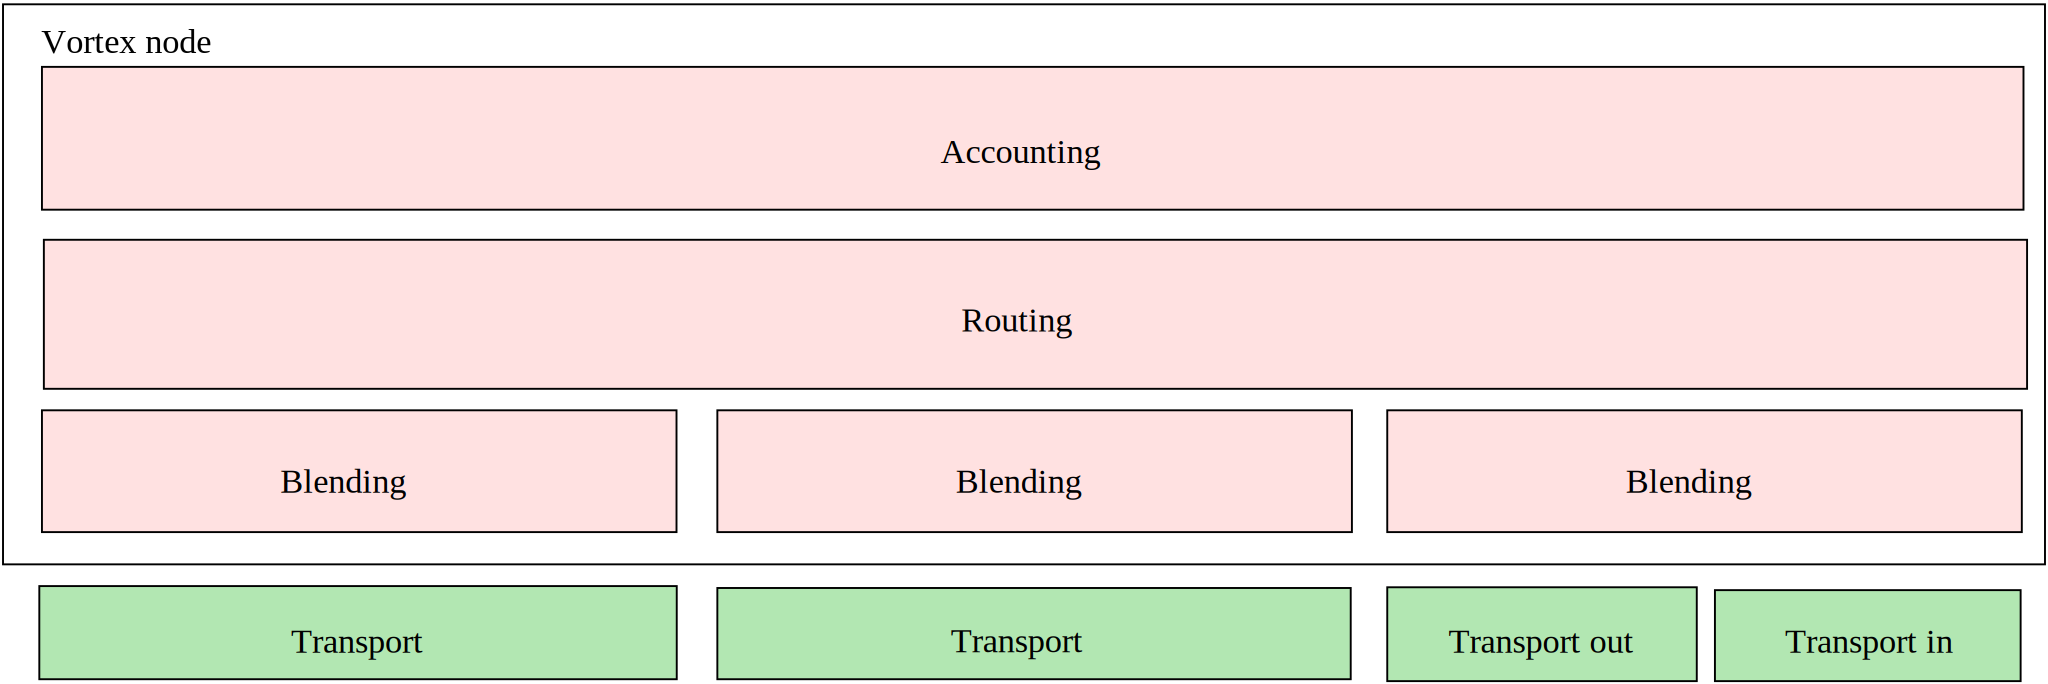
\includegraphics[width=\textwidth]{inc/layerDesign}
	\caption{The protocol layers}
	\label{fig:protocolLayers}
\end{figure}

The protocol is a four-layer protocol, as shown in figure~\ref{fig:protocolLayers}. We communicate with standard protocols, which we refer to as the transport layer. While included in the message flow, they do not form a part of the \VortexNode. The \VortexNode{} itself consists out of the three layers ``Blending'', ``Routing'', and ``Accounting''.

The blending layer is the bridging part linking a transport layer to the \VortexNode{}. It injects and extracts messages from the transport layer and passes the extracted messages to the routing layer. It may be either used as a protocol bridge (e.g., in the case of XMPP) or act as a sophisticated router (e.g., in the case of the email protocols, where mails are fetched or received on push event via POP3 or IMAP while sending messages using SMTP).

The routing layer receives unified standard messages from the blending layer processes them, possibly extracts messages for local delivery, and passes subsequently created messages to the blending layer.

This design is definitely implementable on a consumer device. On the other hand, it is scalable and suitable for a clustered environment. Blending can be done in a stateless manner, is even suitable for serverless computing, and thus largely scalable. Routing may be implemented either with horizontal partitioning along with a set of \defref{eID}s or on a serverless base with a unified storage in the background. The accounting layer acts as a controller and may be implemented as well as stateless service with a minimal NOSQL-storage for all \defref{eID}s. 

\chapter{Protocol}\label{sec:protocol}
\MessageVortex{} is a protocol piggybacking standard transport protocols somehow similar to S/MIME\cite{rfc2015} or PGP\cite{PGP}. Unlike these protocols, we need the capability to keep the presence of our messages secret.  The message itself should only be visible to an intended node.\MessageVortex{} itself is agnostic to the transport, but we do require appropriate blending to hide within the transport protocol. The information processed on a node and its associated meta-information should not leak any information about the processed message. 

Our system sends so-called \VortexMessages. These messages are hidden within a transport protocol (e.g., SMTP or XMPP) with a blending mechanism (e.g., the steganographic algorithm F5) and extracted by a blending layer. The extracted \VortexMessage{} is handed over to a routing layer. The \VortexMessage{} itself contains a header block, a routing block, and possibly some payload blocks. The header block contains all the information required to protect the system. The routing block contains instructions (so-called "operations") how the payload blocks have to be processed and where to send the resulting blocks. Those operations are one of the keys as information leaking happens in this step in most of the systems. We, therefore, crafted all operations very carefully to keep as much information secret as we could. These operations are the key to the system as they allow us to increase and decrease the size of a message without leaking what part of the data is a decoy and what not.

A payload may either be kept by the system for later processing with other messages, processed (possibly with different) payload blocks, or displayed to the "local user" as a message.

The general idea of the protocol is to form a network from nodes that mix and route messages between the sender and receiver. A routing block builder (\defref{RBB}), which is typically identical to the sender, has full control over almost all attributes of the message, and nodes are unable to learn anything from the message while routing. Each user has a node, and there may be additional nodes (public routing nodes) without a user connected to it. 

The message is either onion-like encrypted, split into parts and remerged, or blown up with redundancy information. 

This behavior results in a mixing like a system with a decoy generation in which even decoy generating nodes are unable to differentiate between real traffic and decoy as all blocks always contain parts of the message. Routing decisions are controlled by the builder of the routing block, and redundancy is possible and controlled by the routing block builder to make the system more stable.

In the following sections, we describe this protocol in detail. First, we build a terminology implicitly used in the previous chapters. Then we describe the key concepts and techniques of the protocol without in-depth analysis or reasoning. Implementation and operational aspects are discussed in part~\ref{sec:implementation} and part~\ref{sec:operation}. 


\section{Protocol Terminology}
For our protocol, we use the following terms:
\begin{itemize}
	\item \textbf{\defref{Sender}:} The user or process originally composing the message.
	\item \textbf{\defref{Recipient}:} The user or process destined to receive the message in the end.
	\item \textbf{\defref{User}:} Any entity, running a \MessageVortex{} node.
	\item \textbf{\defref{Router}:} Any node which is processing the message. Please note that all \VortexNode{}s are routers. This includes the senders' and recipients' node.
	\item \textbf{\defref{Message}:} The "real content" to be transferred from the sender to the recipient.    
	\item \textbf{\defref{VortexMessage}:} The encoded message passed from one node to another one. The \VortexMessage{} is considered before any embedding takes place. If embedded, we refer to such a message as "embedded \VortexMessage".
	\item \textbf{\defref{Payload}:} Any data transported in a \VortexMessage{} between routers with exception to the routing and header block, regardless of the meaningfulness or relevance to the \VortexMessage.
	\item \textbf{\defref{Decoy traffic}:} Any payload transported between routers that have no relevance to the message at the final destination.
	\item \textbf{\defref{Identity}:} A tuple of a routable address and a public key. This tuple is a long-living tuple but may be exchanged from time to time. An Identity is always assigned to a nod, but one node may have multiple identities. 
	\item \textbf{\defref{eID}:} An identity created on any node with a limited lifetime anyone possessing the private key (proven by encrypting with it) is accepted as representative of that identity.
	\item \textbf{Routing Block Builder (\defref{RBB}):} An entity, which is building a routing block. Typically identical to either sender or recipient.
\end{itemize}

\section{Key Components}
The following sections list some of the key components of the system. Their understanding is essential for the understanding of the protocol as a whole. 

We first describe a single node and its identity. This node is always equivalent to a potential recipient. 

We then introduce the concept of workspaces and ephemeral identities. These concepts are essential for the routing and accounting layers. They dictate memory and storage requirements and lay a foundation for the routing layer.

A node always consists of three layers and one or more transports connected to it. The understanding of their inner workings is essential to the understanding of the project as a whole. We emphasize on their main function and their inner workings without going into implementation details. These details are further discussed in part~\ref{sec:implementation}. We mainly focus on the data and the high-level processing done within these layers.

\subsection{Nodes and their identities}
We refer to a \VortexNode{} (node) as a system run by an individual containing a processing software processing \VortexMessages. Each node is connected to a transport layer protocol service (e.g., an IMAPv4 server as an endpoint for email or an XMPP server). 

Each node $o$ has at least one identity reflected by an asymmetric key pair $K_{host_o}$. Any node $p$ communicating with node $o$ must have the public key  $K^1_{host_o}$ of the node.

A node requires the key $K^1_{host_o}$ to encrypt a message for node $o$. This key know-how enables environments with censoring adversaries to withstand probing attacks, as, without the knowledge of such keys, no reply from a node is received. The transport endpoint itself is not secret. The usage as \VortexNode, however, is kept secret as long as the key is not known.

The protocol itself has the possibility to answer clear-text requests. So-called ``public nodes'' (see \ref{sec:vortexNodeTypes}) make use of such messages. They are, however, an exception. In general, all \VortexMessages{} are encrypted.

\subsection{Workspaces and Ephemeral Identities}
We dumped the approach for a system global unified storage for all message processing as such a design would allow an adversary to flood our storage. Instead, we introduced temporary storages suitable for a set of transaction belonging to a single identity or limited set of entities which collaborate. In our system, every transaction on a nose is assigned to an ephemeral identity (\defref{eID}). An \defref{eID} has a limited lifetime and is represented by an asymmetric key pair and has to be created on each \VortexNode{} taking part in a message processing. Each \defref{eID} has a storage assigned to which we refer as ``workspace''.

An \defref{eID} is unique on every host and created on each \VortexNode{} by the routing block builder (\defref{RBB}). To create an \defref{eID}, an \defref{RBB} first sends a message with only a header block to the respective \VortexNode. The request contains the new identity, a reply block, and a request to create a new identity. The receiving \VortexNode will then typically sends a challenge back. A challenge may be the start of a hash bit sequence (also referred to as "puzzle"). The requester has then to resend the request with a header block. The requester must insert additional data in such a way that the start hash in its binary form matches the bit sequence provided. Another possibility is to request a payment in cryptocurrency. This allows us to commercialize routers in some countries where the usage of such routers is generally allowed.

The length of the requested bit sequence is chosen by the accounting layer at its own will. If the request is not answered in a given time, the \defref{eID} will be discarded. Analogous to an SYN-Flood attack, an adversary may try to overwhelm a \VortexNode{} with \defref{eID} creation requests. Such flooding will be much more costly for the adversary than for the \VortexNode{}, and such a node may decide to temporarily no longer accept new \defref{eID} requests without affecting already existing \defref{eID}s.

Each \defref{eID} has a lifetime, a maximum number of messages to be processed, and a maximum number of bytes to be sent assigned to it. The lifetime of an \defref{eID} is typically days and maybe up to a low number of months. Lifetimes may not be extended and are defined by the sender of the request. A node may accept or decline the request if the lifetime of the request or the state of the node does not meet its expectation. The puzzle sent in return may be a fixed value or related to the nodes' current state and load.

This system guarantees that a sender must invest considerable work (in terms of CPU time required) prior to using resources of a \VortexNode. A \VortexNode{} may raise the complexity of its puzzles when having a  high load. This allows for a single user to still obtain an \defref{eID} while increasing costs for an attacker considerably. Even if someone floods a node with new \defref{eID}s, already created \defref{eID}s are not affected as their workspace has already been allocated.

The workspace itself contains chunks of the messages (payload blocks) mapped to IDs and operations. The Operations transform one or more source IDs onto one or more target IDs. Any of these payload blocks may be assigned to a subsequent message as payload block by a routing block. An operation or a payload block share the lifetime of the respective message header. If operations overlap in output blocks the newest operation (arrived latest) wins.

This concept has certain downsides related to the expiry of \defref{eID}s. We will address them in section\ref{sec:newEID} and section~\ref{sec:replaceMURB}.

\subsection{Protocol Layers}
As already introduced in \ref{sec:reqSummary}, the protocol is built on multiple software layers. On the logic side, the protocol is split into two parts:
\begin{enumerate}
	\item Transport Layer\\
	Standard Internet infrastructures provide this layer. The primary goal is to hide or blend our protocol into regular traffic within that layer. Typical examples for such layers are SMTP or XMPP servers.
	\item Blending and subsequent layers (the Vortex infrastructure)\\
	Any user of the Internet may provide these layers. Since these layers may be only Vortex routing nodes or valid endpoints, the nodes may or may not be publicly known. In a first implementation, we build this system as a standard Java application. The primary goal is to compile it to native code afterward and run it on an SoC like infrastructure such as a RaspberryPi or port it to an android device.
	
	We may further split the Vortex infrastructure layers into
	\begin{enumerate}
		\item Blending layer\\
		This layer receives messages from the Vortex system and creates transport layer conformant messages and vice-versa. In an ideal case, the messages generated by this layer are indistinguishable from any regular message traffic of the transport layer, and the embedded message is only detectable by the receiving node.
		\item Routing layer\\
		The routing layer disassembles and reassembles messages. 
		\item Accounting layer\\
		The accounting layer has three jobs. First, he has to authorize the message processing after the decryption of the header block by the blending layer. Secondly, he handles all header request blocks and the reply blocks. And third, it keeps track of the accounting regarding the sent messages. Its main purpose is to protect the system from misuse or flooding.    
	\end{enumerate}
\end{enumerate}

In total, we have four layers. The bottom-most layer consists of unmodified standard infrastructure for transport within the Internet, and the three layers on top build a single \VortexNode.

\subsection{Transport Layer}
The transport layer is a standard protocol within the Internet. It is neither a \MessageVortex{}-specific infrastructure, nor has it been modified for the purpose. Instead, it serves the purpose as a store and forward medium. This medium solves two major problems. First, no NAT traversal technology such as "TCP hairpins" or "hole punching" is required. And secondly, it compensates for short outages due to regional routing problems to the end-user.

A transport layer should have some generic properties:
\begin{itemize}
	\item Widely adopted 
	\item Reliable
	\item Symmetrical built 
\end{itemize}

For a more detailed description of the criteria, see section~\ref{sec:transportCriteria}.

For our first tests, we used a custom transport layer, allowing us to monitor all traffic quickly, and build structures in a very flexible way. This transport layer works locally or in a broadcast-based network with a minimum amount of work for setup and deployment. The API we used may, however, be used to support almost any kind of transport protocol.

In section~\ref{sec:transportProtocols}, we make a short analysis going through some common protocols outlining the strength and weaknesses of common transport protocols within the Internet.

After that, we focussed on the protocols identified in the previous sections for transport:
\begin{itemize}
	\item \defref{SMTP}
	\item \defref{XMPP}
\end{itemize}
For the prototype, we have implemented an SMTP transport agent and the respective blending layer.

\subsubsection{Blending Layer\label{sec:blendingLayer}}
The blending layer is taking care of multiple problems:
\begin{itemize}
	\item It is translating the message block into a suitable format for transport\\
	This translation includes jobs such as embedding a block as encoded text, as a binary attachment or hide it within a message using steganography. Another demanding task in this context is to create credible content for the transport message itself.
	\item Extract incoming blocks\\
	Identify incoming messages containing a possible block and extract it from the message.
	\item Do housekeeping on the storage layer of the transport protocol\\
	Access protocols such as POP and IMAP require that messages are deleted from time to time to stay below the sizing quotas of an account. To manage this transport layer account is the job of the blending layer.
\end{itemize}

There is no specification on the housekeeping part of the blending layer, as this part is specific to the requirements of the account owner. We do, however, recommend to handle messages precisely as if the messages would be handled on an account handled by a human. This means that some messages. 

The blending is currently done by merging the \VortexMessage using either F5 as described in \cite{f5} or by doing plain blending, which is a binary embedding. This means that we require jpeg images included in the SMTP message. 

\paragraph{Processing of a Message received from the Transport Layer}~\\
We define the blending layer to work as follows when receiving messages:
\begin{enumerate}
	\item Log arrival time on the transport layer.
	\item Extract possible \VortexMessage.
	\item Apply decryption on a suspected header block of \VortexMessage.
	\item Identify the header block as valid by querying the accounting layer.
	\item Extract and decrypt subsequent blocks.
	\item Pass extracted blocks and information to the routing layer.
\end{enumerate}

\paragraph{Processing of a Message received from the Routing Layer}~\\
We define the blending layer to work as follows for sending messages:
\begin{enumerate}
	\item Assemble message as passed on by the routing layer.
	\item Using the blending method specified in the routing block, build an empty message. 
	\item Create a message decoy content.
	\item Send the message to the appropriate recipient using the transport layer protocol.
\end{enumerate}

\paragraph{Credible Content Creation for the Transport Layer}~\\
One of the most demanding tasks of the blending layer is to create transport protocol messages. In \cite{oakland2013-parrot}, \citeauthor{oakland2013-parrot} expresses that it is easy for a human to determine decoy traffic as the content is easily identifiable as generated content. While this is up to all that we know true, there is a possibility here to generate "human-like" data traffic to a certain extent. For the blending layer, it is not necessarily required to mimic human messages. Instead, the blending layer may generate messages such as password recovery messages, monitoring messages, and even \defref{UBE}-like content. All these messages have required properties in common. First, all of them are machine-generated messages which are modified quite often. All of these messages are known to be sent and possibly adapted individually. 

For the blending itself, we required a steganographic algorithm. After reviewing the options, we decided to go for F5\cite{f5} as a steganographic algorithm. It is a reasonably well-researched algorithm, which attracted many researchers. The original F5 implementation had a detectable issue with artifacts\cite{F5broken} caused by the recompression of the image. This issue was caused only due to a problem in the reference implementation, and the researchers have provided a corrected reference implementation without the weakness.

We looked for other steganographic algorithms, but were unable to find any other suitable algorithm apart from F5, which fulfilled the following set of criteria:
\begin{itemize}
	\item Unbroken.
	\item Researched.
	\item Suitable for embedding in lossy compressed, common image formats (e.g., jpeg).
	\item An implementation or a well-specified algorithm exists.
\end{itemize}

We decided to keep our plain embedding algorithm in the implementation. It already requires an in-depth analysis or a human to detect embedding, and the message itself is, even if detected, well-protected. Its biggest most strength is, however, its efficiency. This algorithm is, however, only suitable for public nodes matching up to an observing adversary (as defined in section~\ref{sec:adversary}). It must not be used in environments where a censoring adversary is suspected.

When using F5, jpeg images are required. Imagery requires to be at least eight times the size of the message embedded. Unlike other approaches harvesting random pics or obtaining them from a local repository, we recommend using machine-generated images such as rendered content. We recognize that custom Gravatars, router and usage graphs of services, or render services are suitable imagery material for our purpose. The message content would obviously be machine-generated content and not being suspect. This would effectively render the dead parrot problem as described in \cite{oakland2013-parrot} ineffective. 

\subsubsection{Routing Layer\label{sec:routingLayer}}
A routing layer needs to receive all payload and routing blocks, and process them (For an exact outline of the routing block, see section~\ref{sec:vortexMessage}). These blocks are stored in a suitable list within the workspace of the eID identified by the header block.

Within the routing block, we find a set of instructions, next \VortexNodes information, and the encrypted routing blocks for the messages to be assembled. A simplified representation of a routing block is shown in figure~\ref{fig:mathRoutingSimplified}.

\begin{figure}[!ht]
	\begin{align}
	\mathbf{ROUTING_o}           = & \langle [ \mathbf{ROUTINGCOMBO} ] *, \mathbf{replyBlock},operation* \rangle\\  
	\mathbf{ROUTINGCOMBO}        = & \langle processIntervall, K_{peerN+1}, recipient, \mathbf{nextMP}, \mathbf{nextHP}, \nonumber \\
	& \mathbf{nextHEADER}, \mathbf{nextROUTING}, \mathbf{assemblyInstructions} \rangle\\
	\mathbf{PL}                  = & \langle \text{payload octets} \rangle *\\ 
	\mathbf{nextMP}              = & E^{K^1_{host_{o+1}}} \left( K_{peer_{o+1}} \right)\\
	\mathbf{nextHP}              = & E^{K^1_{host_{o+1}}} \left( K_{sender_{o+1}} \right)\\
	\mathbf{nextHEADER}          = & E^{K_{sender_o}} \left( \mathbf{HEADER_{o+1}} \right)\\
	\mathbf{nextROUTING}         = & E^{K_{sender_o}} \left( \mathbf{ROUTING_{o+1}} \right)\\    
	\mathbf{operations}          = & \langle \text{list of operations} \rangle \\
	\mathbf{assembyInstructions} = & \langle  blendingInformation, nextHop, \langle \text{mapping operation} +\rangle \rangle
	\end{align}
	\caption{Simplified representation of a routing block}
	\label{fig:mathRoutingSimplified}
\end{figure}

The routing of a message is simple. A workspace of an \defref{eID} contains routing blocks and payload blocks. A routing block has an active time window defined in the header block. Anytime during that time window, a routing layer processes the routing instructions contained in the assembly operations of the routing block. If successful, the message will be sent using the specified blending layer and target address.

The routing layer stores the main information assigned to the operation of routing messages. The following data has to be kept for routing within the \defref{eID}s workspace:
\begin{itemize}
	\item $\mathbf{Build[]}\langle expiry, buildOperation \rangle$\\
	The array $\mathbf{Build[]}$ is a list of building instructions for a message. The server may decide at any time to reject a too big list or long-living message. Thus, he may control the size of this list as well. However, controlling the size of this list will most likely result in the non-delivery of a message. 
	
	The $buildOperation$ is extracted by enumerating $operation*$ while $expiry$ is the upper bound of the $processIntervall$.
	\item $\mathbf{Payload[]}\langle expiry, payload, id \rangle$\\
	The array $Payload[]$ reflects a list of all currently active payloads. Servers may decide to store derivatives of payloads. However, as derived payloads inherit their expiry from the generating operation, such behavior may be safely omitted and operations executed if their result is required.
	
	\item $\splitatcommas{\mathbf{Route[]}\langle processIntervall, blendingInformation, nextHop, \mathbf{nextMP}, \mathbf {nextHP}, \mathbf{nextHeader}, \mathbf{nextRouting}, K_{peer_{o+1}}, \mathbf{assemblyInstructions} \rangle}$\\
	The list of routing information triggers processing. At a randomly chosen time defined in the $processIntervall$, a message is composed. The message is assembled by doing $\splitatcommas{\langle \mathbf{nextMP}, E_{K_{peer_{o+1}}}\langle \mathbf{nextHP}, \mathbf{nextHEADER}, \mathbf{nextROUTING}, payload* \rangle \rangle}$. The payloads are created with the help of the arrays $build[]$ and $payload[]$, and as soon as the message is authorized by accounting and passed to the blending layer, the entry in this list is discarded.
\end{itemize}

\subsubsection{Accounting Layer\label{sec:accountingLayer}}
The accounting layer keeps tracks of all information required assigned to ephemeral identities (\defref{eID}). It is queried by the blending Layer and routing Layer for authorization of the operations. The accounting layer manages the following tuples of information:

% List duplicated in Accounting layer in implementation and protocol
\begin{itemize}
	\item $\mathbf{eID[]}\langle expiry, pubKey, mesgsLeft, bytesLeft \rangle$\\
	The $\mathbf{eID}$ tuple is the longest living tuple. It reflects an ephemeral identity and exists as long as the current identity is valid. All other tuples are short living lists. As the server decides if he accepts new identities or not, the size of this data is controllable. 
	\item $\mathbf{Puzz[]}\langle expiry, request, puzzle \rangle$\\
	The array $\mathbf{Puzz[]}$ is a list of not yet solved puzzles of this \defref{eID}. Every puzzle has a relatively short lifespan (typically below 1d). A routing node controls the size of this list by only accepting requests to a certain extent. Typically this list should not surpass two entries as we should have either a maximum of two quota requests or one identity creation request open.
	\item $\mathbf{Replay[]}\langle expiry, serial, numberOfRemainingUsages \rangle$\\
	The array $\mathbf{Replay[]}$ is a list of serials. List entries are created upon their first usage and remain active until the block is expired. 
\end{itemize}


\subsection{VortexMessages}\label{sec:vortexMessage}\index{VortexMessage}
A \VortexMessage{} is built by combining multiple loosely interconnected blocks. We first name the blocks and their function, and then we explain the inner working of the blocks and do some reasoning why the block has been built as it is. 

Figure~\ref{fig:messageOutline} shows an outline of the block structure of a message destined to $host_o$. For a mathematical representation, see figure~\ref{fig:mathMessage}.

\begin{figure}[ht]
	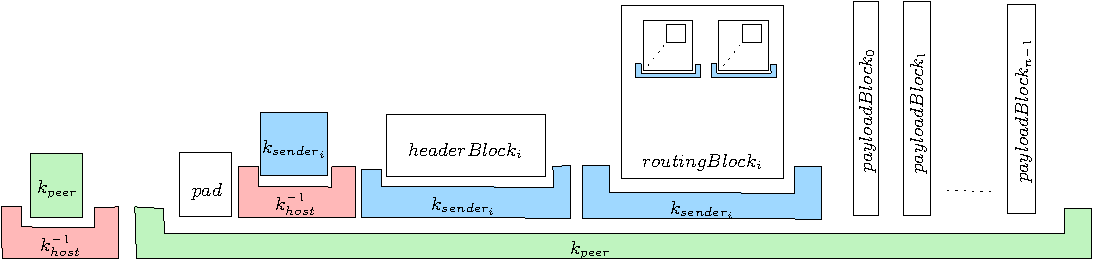
\includegraphics[width=\textwidth]{inc/blockLayoutSimplified}
	$\splitatcommas{\langle \mathbf{MPREFIX_o}, E_{K_{peer_{o+1}}}\left( \mathbf{HPREFIX_o}, \mathbf{HEADER_o}^{K_{sender_o}}, \mathbf{ROUTING_o}^{K_{sender_o}}, payload* \right) \rangle}$
	\caption{Simplified message outline visually and in math}
	\label{fig:messageOutline}
\end{figure}

The first block is the message prefix block $\mathbf{MPREFIX_o}$, which has been encrypted with the public key of the receiving node $K^1_{host_o}$. This block contains the key for decrypting the whole rest of the message. Each PREFIX block contains a symmetrical ey and the specification on how to encrypt or decrypt with it (mode, padding, IV, and other possibly required parameters) in ASN.1 encoding. 

Immediately following the message prefix block, we have the inner message block. This message blocks contain three more blocks and a variable number of payload blocks. The inner message is encrypted with the symmetrical peer key $K_{peer_o}$. This peer key is specific to this message and nowhere reused. It is only known by the two peer hosts $host_o$ and $host_{o-1}$, and the routing block builder (\defref{RBB}). More importantly, $host_{o-1}$ does not need to know the host key of $host_o$. Therefore, relaying a message to $host_o$ does not enable $host_{o-1}$ to communicate with $host_o$. 

The blocks $HEADER_o$ and $ROUTING_o$ are protected with an additional key $K_{sender_o}$. The decryption key is obtained by $host_o$ from the header prefix block $\mathbf{HPREFIX}$. After only decrypting the header block $\mathbf{HEADER}$ and verifying its signature, the accounting layer may check if further processing is authorized. The splitting of the two keys allows us to\ldots
\begin{itemize}
	\item \ldots send a message to $host_o$ without $host_{o-1}$ knowing the host key of $host_o$.
	\item \ldots hide the structure of the message itself.
	\item \ldots keep the content of $\mathbf{HEADER_o}$, and $\mathbf{ROUTING_o}$ secret from $host_{o-1}$.
\end{itemize}

After authorization by the accounting layer, the header block is processed as outlined in section~\ref{sec:processingIncommingMessages}. Basically, we just add the routing blocks and payload to the respective workspace and wait for the routing layer to process the information.

Looking at a full \VortexMessage, we get the protocol outline, as shown in \eqref{eq:vortexMessage} on page~\pageref{eq:vortexMessage}.

\begin{figure*}[!ht]
	\begin{align}
	\mathbf{VORTEXMESSAGE}       = &\langle \mathbf{MP}^{K^{-1}_{host_o}}, INNERMESSAGE \rangle \label{eq:vortexMessage} \\ 
	\mathbf{INNERMESSAGE}        = &\langle \mathbf{CP}^{K^{-1}_{host_o}}, \mathbf{H}^{K_{sender_o}}, E^{K^{-1}_{sender_o}}\left(H\left(\mathbf{HEADER}\right)\right), \left[\mathbf{R}^{K_{senderN}}\right], \left[\mathbf{PL}\right]*\rangle^{K_{peerN}} \label{eq:innerMessage}\\
	\mathbf{MP}^{K^{-1}_{hostN}} = &E^{K^{-1}_{hostN}}\left(\mathbf{PREFIX}\langle K_{peerN}\rangle \right)\\ 
	\mathbf{HP}^{K^{-1}_{hostN}} = &E^{K^{-1}_{hostN}}\left(\mathbf{HPREFIX}\langle K_{senderN}\rangle \right)\\ 
	\mathbf{H}^{K_{senderN}}     = &E^{K_{senderN}}\left(\mathbf{HEADER}\right)\\  
	\mathbf{HEADER}              = &\langle K^{1}_{senderN}, serial, maxReplays, validity, [requests, requestRoutingBlock],\nonumber\\ 
	& [puzzleIdentifier, proofOfWork] \rangle \\  
	\mathbf{R}^{K_{senderN}}     = & E^{K_{senderN}}\left(\mathbf{ROUTING}\right)\\ 
	\mathbf{ROUTING}             = & \langle [ \mathbf{ROUTINGCOMBO} ] *, forwardSecret, \mathbf{replyBlock},\mathbf{operations} \rangle\\  
	\mathbf{ROUTINGCOMBO}        = & \langle processIntervall, K_{peerN+1}, recipient, \mathbf{nextMP}, \mathbf{nextHP}, \nonumber \\
	& \mathbf{nextHEADER}, \mathbf{nextROUTING}, \mathbf{assemblyInstructions} \rangle\\
	\mathbf{nextMP}              = & E^{K^1_{host_{o+1}}} \left( K_{peer_{o+1}} \right)\\
	\mathbf{nextHP}              = & E^{K^1_{host_{o+1}}} \left( K_{sender_{o+1}} \right)\\
	\mathbf{nextHEADER}          = & E^{K_{sender_o}} \left( \mathbf{HEADER_{o+1}} \right)\\
	\mathbf{nextROUTING}         = & E^{K_{sender_o}} \left( \mathbf{ROUTING_{o+1}} \right)\\    
	\mathbf{operations}          = & \langle \text{list of operations} \rangle \\
	\mathbf{assembyInstructions} = & \langle  blendingInformation, nextHop, \langle \text{list of mapping operations}\rangle\rangle\\
	\mathbf{PL}                  = &\langle \text{payload octets} \rangle *\\ 
	\end{align}
	%\captionsetup{labelformat=empty}
	\caption{Detailed representation of a VortexMessage}
	\label{fig:mathMessage}
\end{figure*}

The routing log block is an onionized block. It contains at least a $forwardSecret$, which must match up with the header blocks $forwardSecret$. This mechanism is required to guarantee that routing blocks are not exchanged. The $replyBlock$ provides a possibility, if provided, to contact the original sender of the message without knowing him. It is just a routing block with instructions on how to prepare the message to be sent. The routing combos contain all the necessary information and prebuilt blocks to create the subsequent messages.

At the very end, we got the payload. These blocks are simply added to the \defref{eID}s workspace.

The double encryption of the routing and header block, are doubly encrypted. We could argue that the inner message block should not be encrypted with a peer key. This looks like a flaw at first sight but is, in fact, a feature that is very important. Without this key, any independent observer with knowledge about the blending capabilities of a receiving node may\ldots
\begin{itemize}
	\item Easier to identify the block structure.\\ 
	This statement remains regardless of whether ASN.1 or length prefixed structures are used. If the structure of a \VortexMessage is easily identified, the messages may be logged or dropped.
	\item Identify the routing block size.\\
	The value of this information is only minimal as it only reflects the complexity of the remaining routing information indirectly.
	\item Identify the number of payload blocks and their respective sizes. \\
	Sizing information is valuable when following the path of a message.
\end{itemize}

\subsubsection{Message Structure Related to Censorship Circumvention}
It is important to note that there is no structure dividing the encrypted peer key from the Inner message block. The size of the peer key block is defined by the key and algorithm of the host key. 

The whole \VortexMessage is, looking from outside, a structureless blob with a maximum of entropy caused by the encryption employed. 

This is intentional and by design. Plain embedding uses furthermore a method of splitting, which allows a message block to be embedded in chunks in carrier information. By design, neither the message nor their embedding display detectable attributes allowing them to identify the message. 

Exactly as with the routing operations, great care has been applied. Any random sequence of bytes may be interpreted as valid chunking. For more exact implementation details on chunking, see section~\ref{sec:chunkingPlain}.

\subsubsection{Message Structure Related to Information Leaking}
From the inside, the $\mathbf{INNERMESSAGE}$ (see \ref{eq:innerMessage}) is built as a structure leaking the absolute minimum of information. A node receiving and decoding the message will learn the following information:
\begin{itemize}
	\item IP of the sender of the transport layer.
	\item The address and embedding schemes of all receiving transport layers.
	\item The size of the payload blocks.
	\item The size of the subsequent routing blocks.
	\item The peer key $K_{peer_o}$.
	\item The size of the prefix blocks.
\end{itemize}

It is unable to extract the following information:
\begin{itemize}
	\item The required keys to communicate with the suspected peer node.
	\item Any information related to message size, content, or recipient.
\end{itemize}

\subsection{Routing Operations\label{sec:operations}}
The routing operations build the core as they define the capabilities of the mixing. We decided to introduce three different classes of operations. Wherever we employ crypto, operations, we may choose the operation required for the operation. No choices exist for the core Reed-Solomon-Function, the padding and spitting operation related to it, and the split and merge operations.

\subsubsection{$addRedundancy$ and $removeRedundancy$ Operations}
I this section we focus on the core operation of our system. The $addRedundancy$ and $removeRedundancy$ allow growing message sizes in our system without allowing to identify the decoy traffic. 

The Lagrange functions have been proposed in \cite{shamir1979share} and further more generalized in \cite{mceliece1981sharing} for sharing secrets. The general idea about all proposed schemes is to distribute informations and restrct access to it so that only if a specified number of shares are captured a secret may be rebulit. Unlike proposed in these papers we do not apply privacy to our protocol by sharing the data among many points. Instead we use lagrange functions to create decoy traffic. By doing so even a creator of traffic is unable to tell message traffic from decoy traffic apart. 

These operations build the core of the routing capabilities of a node. The operation allows an \defref{RBB} to add to a message redundancy information or to rebuild a block from a chosen set of information. 

The operation itself is shown in figure~\ref{fig:addRedundancyOperation}. 
\begin{figure}[ht]\centering
	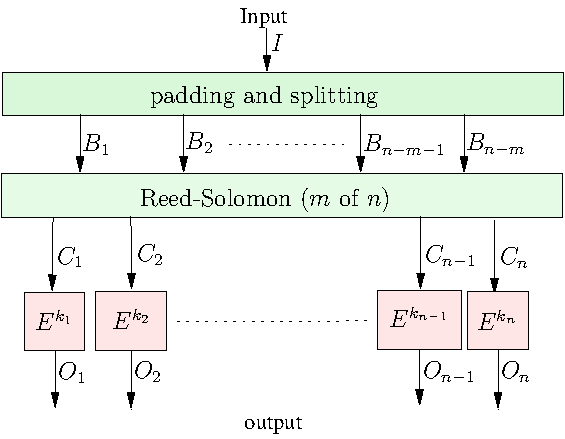
\includegraphics[width=0.8\columnwidth]{inc/addRedundancyOp}
	\caption{Outline of the addRedundancy operation}
	\label{fig:addRedundancyOperation}
\end{figure}

It may be subdivided into the following operations:
\begin{itemize}
	\item Pad the original message block in such a way, that all resulting blocks are a multiple of the block size of the encrypting cipher.
	\item Apply a Reed Solomon operation in a given GF space with a vanderMonde matrix.
	\item Encrypt all resulting blocks with unpadded, symmetrical encryption.
\end{itemize}

The padding applied in the first step is non-standard padding. The reason for this lies in the properties required by the operation. The presence of standard padding may leak, whether the block has been successfully decrypted or not. Therefore, we created a padding with the following properties:
\begin{itemize}
	\item The padding must not leak whether the rebuild cycle of the operation was successful or not.
	\item Anyone knowing the routing block content and the transmitted message must be able to predict any treated block, including all padding bytes.
	\item The padded content must provide resulting blocks of required size to enable non-padded encryption after the RS operation
	\item The padding must work with any size of padding space.
	\item The padded and encrypted block must not leak an estimate of the original content.
\end{itemize}

The padded block $\mathbf{X}$ is created from a padding value $p$, the unpadded block $\mathbf{M}$ and a series of padding bytes. We build $\mathbf{X}$ for a function $RS_{\text{m of n}}$ (allows adding $m$ redundancy blocks) and an encryption block $\mathbf{M}$ sized $K$ as follows:
\begin{eqnarray}
i          & = & len(\mathbf{M})\\
e          & = & k \cdot n\\
l          & = & \left\lceil\frac{i + 4 + C2 }{e}\right\rceil\cdot e\\
p          & = & i + \left( C1 \cdot l \pmod{\left\lfloor\frac{2^{32}-i}{l}\right\rfloor\cdot l}\right)\\
\mathbf{X} & = & \langle p,\mathbf{M},R_{t}\left(s,l-i-4\right)\rangle
\end{eqnarray}    
The remainder of the input block, up to length $l$, is padded with random data. The random padding data may be specified by RBB though a PRNG spec $t$ and an initial seed value $s$. The message is padded up to size $L$. All resulting, encrypted blocks do not require any padding. This because the initial padding guarantees that all resulting blocks are dividable by the block size of the encrypting function. If not provided by an RBB, an additional parameter $C1$ is chosen as random positive integer and $C2=0$  by the node executing the operation.

To reverse a successful message recovery information of a padded block $\mathbf{X}$, we calculate the original message size by extracting $p$ and doing $len(\mathbf{M})=p \pmod{ len(\mathbf{X})}$.

This padding has many important advantages:
\begin{enumerate}
	\item The padding does not leak if the rebuilding of the original message was successful. Any value in the padding may reflect a valid value.
	\item Since we have a value $C2$, the statement that a message size is within $len(\mathbf{X})<size<(len(\mathbf{X})-k\cdot n)$ is no longer true and any value smaller $len(\mathbf{X})-k\cdot n$ may be correct as well.
	\item An RBB may predict the exact binary image of the padded message when specifying $C1$, $C2$, and $R_{t}(s,)$.
	\item A node knowing the original parameters $C1$, $C2$, and the initial PRNG seed $s$ can detect successful decryption.
\end{enumerate}

Apart from being non-standard padding, the padding has additional downsides:
\begin{itemize}
	\item The padding is inefficient compared to simple paddings such as PKCS\#7
	\item The padding requires an initialized PRNG to generate the padding.
	\item Depending on the chosen parameters, the padding overhead may become significant. 
\end{itemize}

After the padding, the date is ready for the Reed-Solomon part of the operation. We first group the data vector into a matrix $\mathbf{A}$ with $m$ columns to do the operations efficiently. The previous padding guarantees that all columns have a length, which is dividable by the block size of the encryption step applied later.

\begin{eqnarray}
t          & = & n-1\\in bytes
\mathbf{A} & = & vec2mat\left(\mathbf{X},\frac{len\left(\mathbf{X}\right)}{m}\right)\\
\mathbf{V} & = & \left(\begin{matrix}
0^0 & 0^1 & 0^2 & \cdots & 0^{(m-1)} \\
1^0 & 1^1 & 1^2 & \cdots & 1^{(m-1)} \\
2^0 & 2^1 & 2^2 & \cdots & 2^{(m-1)} \\
\vdots & \vdots & \vdots & \ddots & \vdots \\
t^0 & t^1 & t^2 & \cdots & t^{(m-1)}
\end{matrix}\right)\\
\mathbf{P} & = & \mathbf{V}\mathbf{A} \left(GF\left(2^\omega\right)\right)\\
\langle \mathbf{Q_1}, \ldots , \mathbf{Q_n} \rangle & = & row2vec(P)\\
R_i & = & E^{K_i}\left(Q_i\right)
\end{eqnarray}    

We apply the Reed-Solomon function by employing a Vandermonde matrix ($\mathbf{V}$). We build the data matrix ($\mathbf{A}$) by distributing the data into $\frac{len\left(\mathbf{X}\right)}{m}$ columns. This results in a matrix with $m$ rows. Unlike in error-correcting systems, we do not normalize the matrix so that the result of the first blocks is equivalent to the original message. Instead, the error-correcting information is distributed over all resulting blocks ($\mathbf{Q_i}$). Since the entropy of the resulting blocks is lowered as shown in figure~\ref{fig:entropy} and may thus leak an estimate of how a resulting block may have been treated, we added the encryption step to equalize entropy again. The previously introduced padding guarantees that there is no further padding on block-level required. The key used to encrypt the single blocks must not be equivalent. Equivalent keys have the side effect encrypting equal blocks into the same cyphertext. We observed faint but statistically relevant reminders of the unencrypted graphs when treating the same block with the same key and different redundancy parameters.

\subsubsection{$encrypt$ and $decrypt$ Operations}
The encrypt and decrypt operations are essential for the requirement that tagging should not be possible. Unlike the $addRedundancy$ and $removeRedundancy$, the splitting operations do not feature any encryption step after splitting or merging. Reusing a payload block that has only been split or merged would repeat the payload pattern on multiple nodes during transfer. That is why we require to have encryption.

The reason for not building this step into the split and merge function was simple. We needed a separate encryption step to be able to work as an onionizing system, and there were use cases where integrated encryption did not make sense. For further details on this topic, see section~\ref{sec:routingStrategies}.


\subsubsection{$mergePayload$ and $splitPayload$ operation}
The $splitPayload$ operation splits a payload block into two chunks of different or equal sizes. The parameters for this operation are:

\begin{itemize}
	\item source payload block $pb_1$
	\item fraction $f$\\
	A floating-point number which is describing the size of the first chunk. If the fraction is "1.0", then the whole payload is transferred to the second target chunk
\end{itemize}

If $len(pb_1)$ expresses the size of a payloadblock called $pb_1$ in bytes, then the two resulting blocks of the SpitPayload Operation $pb_2$ and $pb_3$ have to follow the following rules:

\begin{eqnarray}
split(f, pb_1) & = &\langle pb_1, pb_2 \rangle\\
pb_1.startsWith(pb_2)\\
pb_1.endsWith(pb_3)\\
len(pb_2) & = & floor(len(pb_1)\cdot f)\\
len(pb_1) & = & len(pb_2) + len(pb_3)
\end{eqnarray}

The $mergePayload$ operation combines two payload blocks into one. The parameters for this operation are:

\begin{itemize}
	\item first source payload block $pb_1$
	\item second source payload block $pb_2$
\end{itemize}

If $len(pb)$ expresses the size of a payloadblock called $pb$ in bytes then resulting block of the MergePayload Operation $pb_3$ have to follow the following rules:

\begin{eqnarray}
merge(pb_1, pb_2) & = & pb_3 \\
pb_3.startsWith(pb_1)\\
pb_3.endsWith(pb_2)\\
len(pb_3) & = & len(pb_1) + len(pb_2)
\end{eqnarray}

Unlike other operations, this operation has no encryption step attached to it. We usually attached an encryption step to remove repeating patterns from the \VortexMessage stream.

It has to be mentioned that this operation tuple has some issues when it comes to floating-point implementations. They are solvable but had to be specified unexpectedly precisely in order to enable a true cross-platform implementation. For more information regarding the issue and exact implementation, see section~\ref{sec:implOperations}.


\section{Summary}
The \MessageVortex{}-Protocol is split into the four layers "Transport" (a common internet standard protocol), "blending" (extracting and embedding \VortexMessages), "Routing" (A layer reassembling messages according to received instruction), and "Accounting" (Keeps track of all stored data and discards expired information).

All nodes are realized in decentral devices such as computers or mobile phones. Messages are hidden with either plain embedding or (referred) F5 in the transport layer message. The routing layer processes messages by applying operations to messages. Valid operations are encrypt or decrypt a message chunk, split a message chunk into two parts, merge two parts into one, or add or remove redundancy information. The last operation is the most valuable. This operation allows by employing an extended Reed-Solomon-Operation to add decoy traffic to the message flow without enabling a node to identify such traffic. Furthermore, it allows a sender to send parts of a message through multiple chains of routing nodes to a recipient. Each message itself does not leak the message content since depending on the completing block, any message with appropriate length may be valid.

The routing itself is done in a temporarily allocated storage called "workspace", which is tied to an ephemeral identity (\defref{eID}) represented by an asymmetric key pair. To get an \defref{eID}, a sender typically solves a crypto puzzle.







%!TeX program=pdflatex
%!TeX encoding=utf8
%!TeX spellcheck = en_US
%!TeX root = ../../messageVortex.tex

\partepigraph{No matter how hard you work, someone else is working harder.}{Elon Musk, entrepreneur}
\part{Implementation}\label{sec:implementation}
The implementation of our system differs from the academic model in some details. It is foremost more precise than the academic model. Furthermore, it requires a strict definition of the implementation to guarantee the interoperability between different implementations.

This section focuses on the details of our reference implementation in Java. In \cref{sec:selection}, we explain the selection of algorithms used by the protocol in general. We then focus on the implementation of the transport (\cref{sec:transportImplementation}), blending (\cref{sec:blendingImplementation}), routing (\cref{sec:routingImplementation}), and accounting (\cref{sec:accountingImplementation}) layers. We then look at the usability (\cref{sec:usabilityImplementation}) and efficiency (\cref{sec:transportImplementation}). Aspects relevant to the implementations' usability and efficiency are covered in \cref{sec:usabilityImplementation} and \cref{sec:usabilityImplementation}.

\chapter{Algorithms, Encodings, and Protocols Selection}\label{sec:selection}
In this chapter, we choose the following mandatory supported algorithms:
\begin{itemize}
	\item Encoding: ASN.1
	\item Encryption
	\begin{itemize}
		\item AES128/256
		\item Camellia128/256
	\end{itemize}
	\item Modes
	\begin{itemize}
		\item ECB
		\item GCM
	\end{itemize}
	\item Paddings
	\begin{itemize}
		\item PKCS\#1
		\item PKCS\#7
	\end{itemize}
	\item MACs
	\begin{itemize}
		\item SHA256/512
		\item RIPE-MD256
	\end{itemize}
	\item PRNG
	\begin{itemize}
		\item mrg32k3a
		\item blumMicali
	\end{itemize}
\end{itemize}

Where security-relevant, we always choose two independent algorithms. As our protocol has the means of signaling them, we may support additional algorithms without affecting communication while improving the variety of available algorithms.

In the following sections, we emphasize on the choice and the encoding used on the protocol level.

For all algorithms, we apply the following criteria:
\begin{itemize}
	\item Always focus on common standards
	\item Focus on interoperability when selecting standards
	\item Focus on efficiency (wherever possible use simple, parallelizable algorithms)
	\item When sensible and possible, chose at least two unrelated algorithms (e.g., cryptographic algorithms or MACs) based on different mathematical problems
\end{itemize}

\section{Encoding Scheme}
As encoding scheme, we specified ASN.1~\cite{dis19878824}. It is more compact than the initially selected XML-Standard and is very common in telecommunication and encryption (e.g., the representation of X509 is in ASN.1). To maintain interoperability, we choose DER-encoding as it has precisely one possible representation for every value. Such a strict definition of encoding is important when signing or solving puzzles in our case and is required to diagnose message paths.

On the downside, ASN-1-encoding is, unlike XML, unreadable by humans. As we hide the messages, we considered this a minor flaw, as we need to have a constantly-extracting program to see the messages' content.

\section{Cipher Selection}
In this protocol, many encryption and hashing algorithms have to be used. In the following, we explain the choice of these algorithms. 

We decided to define fixed key sizes for symmetric ciphers as we chose block ciphers. For asymmetric ciphers, we encode the key length in the asymmetric ciphers' parameters section. Due to their mathematical differences, they are frequently flexible in their parameters such as key or block sizes. 

\begin{figure}[ht]
	\lstinputlisting[linerange={18-84},language=asn.1,multicols=2]{../../../../application-core-library/src/main/asn/MessageVortex-Ciphers.asn}
	\caption{Definition of the structures related to ciphers.}
	\label{fig:defCiphers}
\end{figure}

From the requirements side, we adhere to the following principle:
First of all, we need a subset of encryption algorithms all implementations may rely on. Defining such a subset guarantees interoperability between all nodes regardless of their origin. 

Secondly, we need to have a spectrum of algorithms so that it may be (a) enlarged if necessary and (b) there is an alternative. If an algorithm (or a mathematical problem class) is broken, we have to withdraw broken algorithms without affecting the function in general. 

Third, due to the onion-like design described in this document, our protocol should avoid asymmetric encryption in favor of symmetric encryption to minimize losses due to the key length and the generally higher CPU-load opposed by asymmetric keys.

If the algorithm is generally bound to specific key sizes (due to S-Boxes or similar constructs), the key length is incorporated into the definition. If not, the key size is handled as a parameter.

The key sizes were chosen so that the key types form tuples of approximately equal strength. The support of Camellia192 and AES192 was defined as optional. However, as they are wildly common in implementations, they have already been standardized as they build a possibility to enhance security in the future.

From these criteria, we chose to use the following keys and key sizes:
\begin{itemize}
	\item Symmetric
	\begin{itemize}
		\item AES (key sizes: 128, 192, 256)
		\item Camellia (key sizes: 128, 192, and 256)
	\end{itemize}
	\item Asymmetric
	\begin{itemize}
		\item RSA (key size: 2048, 4096, and 8192)
		\item Named Elliptic Curves
		\begin{itemize}
			\item secp384r1
			\item sect409k1
			\item secp521r1
		\end{itemize}
	\end{itemize}
	\item Hashing
	\begin{itemize}
		\item sha3-256
		\item sha3-384
		\item sha3-512
		\item RIPE-MD160
		\item RIPE-MD256
		\item RIPE-MD320
	\end{itemize}
\end{itemize}

Within the implementation, we assigned algorithms to a security strength level:
\begin{itemize}
	\item LOW\\
	AES128, Camellia128, RSA1024, sha3-256
	\item MEDIUM\\
	AES192, Camellia 192, RSA2048, ECC secp384r1, sha3-256
	\item HIGH\\
	AES256, Camellia256, RSA4096, ECC sect409k1, sha3-384
	\item QUANTUM\\
	AES256, Camellia256, RSA8192, ECC secp521r1, ntru, sha3-512
\end{itemize}

This allows associating the used algorithms with a strength. This list, however, should only serve the purpose of selecting algorithms for people without cryptological know-how.

\section{Mode Selections}\label{sec:modeSelection}
We evaluated the most common cipher modes for suitability. For \MessageVortex, we focused on modes with parallelizable, random access modes that do not authenticate. In addition to the characteristics mentioned before, the main focus was on whether there is a reasonably tested open implementation in Java.

\begin{figure}[ht]
	\lstinputlisting[linerange={86-95},language=asn.1]{../../../../application-core-library/src/main/asn/MessageVortex-Ciphers.asn}
	\caption{Enumeration definition of modes in ASN.1 with support requirements.}
	\label{fig:defModes}
\end{figure}

Figure~\ref{fig:defModes} shows the selected paddings and their requirement level.

Very important was that we quite often re-encrypt already encrypted content. In theory, a partially broken mode is much less problematic when encrypting already random content. However, these flaws are obvious to a crypto savvy person but are not common knowledge. By always choosing the same mode and only using onionizing schemes, the flaw remains. To avoid this, we eradicated modes such as ECB despite the fact that their simplicity could have been a gain for the protocol if properly handled.

\begin{itemize}
	\item ECB (Electronic Code Book)\\
	ECB is the most basic mode. Each block of the cleartext is encrypted on its own. This results in a big flaw: blocks containing the same data will always transform to the same ciphertext. This property makes it possible to see some structures of the plaintext when looking at the ciphertext. This solution allows the parallelization of encryption, decryption, and random access while decrypting. Due to these flaws, we rejected this mode.
	\item CBC (Cipher Block Chaining)\\  
	CBC extends the encryption by XORing an initialization vector into the first block before encrypting. For all subsequent blocks, the ciphertext result of the preceding block is taken as XOR input. This solution does not allow parallelization of encryption, but decryption may be paralleled, and random access is possible. As another disadvantage, CBC requires a shared initialization vector. As with most IV-bound modes, an IV/key pair should not be used twice, which has implications for our protocol.
	\item PCBC (Propagation Cipher Block Chaining)\\
	CBC extends the encryption by XORing, not the ciphertext but a XOR result of ciphertext and plaintext. This modification denies parallel decryption and random access compared to CBC.
	\item EAX\\      
	We rejected as the mode was analyzed and broken in \citeyear{minematsu2013attacks} in~\cite{minematsu2013attacks}.
	\item CFB (Cipher Feedback)
	CFB is specified in~\cite{dworkin2001recommendation} and works precisely as CBC with the difference that the plaintext is XORed and the initialization vector, or the preceding cipher result is encrypted. CFB does not support parallel encryption as the ciphertext input from the prior operation is required for an encryption round. CFB does however allow parallel decryption and random access.
	\item OFB\\
	\cite{dworkin2001recommendation} specifies OFB and works precisely as CFB except for the fact that not the ciphertext result is taken as feedback but the result of the encryption before XORing the plaintext. This denies parallel encryption and decryption, as well as random access.
	\item OCB (Offset Codebook Mode)\\
	This mode was first proposed in~\cite{rogaway2003ocb} and later specified in~\cite{krovetz-ocb-04}. OCB is specifically designed for AES128, AES192, and AES256. It supports authentication tag lengths of 128, 96, or 64 bits for each specified encryption algorithm. OCB hashes the plaintext of a message with a specialized function $H_{OCB}(\mathbf{M})$. OCB is fully parallelizable due to its internal structure. All blocks except the first and the last can be encrypted or decrypted in parallel.
	\item CTR\\
	CTR is specified in~\cite{lipmaa2000ctr} and is a mixture between OFB and CBC. A nonce concatenated with a counter incrementing on every block is encrypted and then XORed with the plaintext. This mode allows parallel decryption and encryption, as well as random access. Reusing IV/key-pairs using CTR is a problem as we might derive the XORed product of two messages. This problem only applies where messages are not uniformly random such as in an already encrypted block.
	\item CCM\\
	Counter with CBC-MAC (CCM) is specified in~\cite{rfc3610}. It allows for padding and authenticating encrypted and unencrypted data. It furthermore requires a nonce for its operation. The size of the nonce is dependent on the number of octets in the length field. In the first 16 bytes of the message, the nonce and the message size is stored. For the encryption itself, CTR is used. It shares the same properties as CTR. 
	
	It allows parallel decryption and encryption as well as random access.
	\item GCM (Galois Counter Mode)\\
	GCM has been defined in~\cite{mcgrew2004galois}, and is related to CTR but has some major differences. The nonce is not used (just the counter starting with value 1). An authentication token $auth$ is hashed with $H_{GFmult}$ and then XORed with the first cipher block to authenticate the encryption. All subsequent cipher blocks are XORed with the previous result and then hashed again with $H_{GFmult}$. After the last block the output $o$ is processed  as follows: $H_{GFmult}(o\bigoplus (len(A)||len(B))) \bigoplus E^{K^0}(counter_0)$. As a result, GCM is not parallelizable and does not support random access.
	
	The mode was analyzed security-wise in \citeyear{mcgrew2004security} and showed no weaknesses in the studied fields~\cite{mcgrew2004security}. 
	
	GCM supports parallel encryption and decryption. Random access is possible. However, authentication of encryption is not parallelizable. The authentication makes it unsuitable for our purposes. Alternatively, we could use a fixed authentication string.
	\item XTS (XEX-based tweaked-codebook mode with ciphertext stealing)\\
	This mode is standardized in IEEE 1619-2007 (soon to be superseded). A rough overview of XTS may be found at~\cite{Martin2010}. It was developed initially for disks offering random access and authentication at the same time. 
	\item CMC (CBC-mask-CBC) and EME (ECB-mask-ECB)\\ 
	In~\cite{Halevi:2003} \citeauthor{Halevi:2003} introduces a cipher mode which is extremely costly as it requires two encryptions. CMC is not parallelizable due to the underlying CBC mode, but EME is. 
	\item LRW\\
	LRW is a tweakable narrow-block cipher mode described in~\cite{tschorsch:translayeranon}. This mode shares the same properties as EBC but without the same cleartext block's weakness resulting in the same ciphertext. Similar to XEX, it requires a tweak instead of an IV.
\end{itemize}

We decided to mainly use CBC. However, most of the implementations are available and lightweight. We therefore were not as restrictive as usual when defining a minimal set.

\section{Padding Selection}
A plain textstream may have any length. Since we always encrypt in blocks of a fixed size, we need a mechanism to indicate how many bytes of the last encrypted block may be safely discarded. 

We have chosen the paddings outlined in \cref{fig:defPaddings} to be supported.
\begin{figure}[ht]
	\lstinputlisting[linerange={97-104},language=asn.1]{../../../../application-core-library/src/main/asn/MessageVortex-Ciphers.asn}
	\caption{Enumeration definition of paddings in ASN.1 with support requirements.}
	\label{fig:defPaddings}
\end{figure}

\subsection{RSAES-PKCS1-v1\_5 and RSAES-OAEP}
This padding is the older one of the paddings standardized for PKCS1. It is basically a prefix of two bytes followed by a padding set of non-zero bytes and then terminated by a zero byte and then followed by the message. This padding may give a clue if decryption was successful or not. RSAES-OAEP is the newer of the two padding standards. 

\subsection{PKCS7} 
This padding is the standard used in many places when applying symmetric encryption in an up to 256 bit key length. The free bytes in the last cipher block indicate the number of bytes being used. This makes this padding very compact. It requires only 1 byte of available data at the end of the block. All other bytes are defined but not needed.

\subsection{OAEP with SHA and MGF1 Padding} 
This padding is closely related to RSAES-OAEP padding. However, the hash size is larger, and thus the required space for padding is much higher. OAEP with SHA and MGF1 padding is used in asymmetric encryption only. Due to its size, it is essential to note that the last block's payload shrinks to $keySizeInBits/8-2-MacSize/4$.

In our approach, we chose to allow these four paddings. The allowed SHA sizes match the allowed MAC sizes chosen above. It is important to note that padding uses space at the end of a stream. Since we are always using one block for signing, we have to ensure that the chosen signing MAC and the bytes required for padding do not exceed the asymmetric encryption's key size. While this usually is not a problem for RSA as there are keys 1024+ bits required, it is an essential problem for ECC algorithms as there are much shorter keys needed to achieve an equivalent strength compared to RSA. 

\subsection{Honorable Mention: A Padding for \texorpdfstring{$redundancy$}{redundancy} Operations}
We introduced an additional type of padding not related to these paddings. For the $addRedundancy$, we required the following unique properties. Unfortunately, we were unable to find any padding which matched the following properties simultaneously:

\begin{itemize}
	\item Padding must not leak successful decryption\\
	For our $addRedundancy$ operation, we required padding that had no detectable structure, as a node should not be able to tell whether a $removeRedundancy$ operation did generate content or decoy. 
	\item Padding of more than one block\\
	Due to the nature of the operation, it is required to pad more than just one block.
\end{itemize}

This padding is the only one for the $addRedundancy$ and $removeRedundancy$ operations. A specification may be found in \cref{sec:redundancyOperation}.

\subsection{Pseudo Random Number Generator Selection}\label{sec:prng}
For our $addRedundancy$ and $removeRedundancy$ operations, we needed a pseudo random number generator (PRNG). For our implementation, we did not research this part in depth as it seemed irrelevant. The only criterion was that it had to create content indistinguishable from an encrypted message. This criterion arose as we used it for invisibly padding an already encrypted message.

The PRNG used for our implementation is an XORshift+ generator. It is based on the XSadd PRNG~\cite{marsaglia2003xorshift} and passes the bigcrush PRNG test suite. It is a fast, XOR-based PRNG which has two internal 64-bit seed states $s_0$ respectively $s_1$ and is defined as follows:

\begin{eqnarray}
	x & = & s_0\\
	s_0 & = & s_1\\
	x & = & x \oplus ( x \ll 23 )\\
	s_1 & = & x \oplus s_1 \oplus ( x \gg 17 ) \oplus (s_1 \gg 26 )\\
	nextNumber & = & s_1+s_0
\end{eqnarray}

We chose this comparably weak PRNG for practical reasons. It is fast, simple, and is based on operations easy to implement on hardware. As we do not need a cryptographically strong PRNG, it is our primary choice so far. 

As the protocol is heavily dependent on security, we introduced everywhere at least one alternate algorithm that may be used to replace a broken algorithm. 

To have a second choice for the PRNG, we define the Blum--Micali PRNG as described in~\cite{blum1984generate}. This PRNG is cryptographically secure and is defined as follows:

$p$ is prime, and $g$ is a primitive root modulo $p$. $x_0$ reflects the seed state.

\begin{eqnarray}
	x_{i+1}=g^{x_i}\mod p
\end{eqnarray}

This PRNG requires significantly more calculation power than the XORshift+ PRNG. On the positive side, the PRNG is well researched, and we have found no weaknesses documented in academia.

%\subsection{Puzzle Selection}
%\fxwarning{Add content here... maybe old text about PoW-Algorithms}
% Eradicated old text too incomplete and massive work required

\section{Transport Layer Protocol Selection}\label{sec:transportProtocols}
The following sections list common Internet protocols. We analyze those protocols for the fitness as transport layer of \MessageVortex. 

We will identify SMTP and XMPP as suitable transport layer protocols for the \MessageVortex{} approach, as they have all required properties.

All sections are structured the same. We first refer to the protocol or standard and describe it in the simplest possible form. We refer to subsequent standards if required to consider extensions where sensible. We then apply the previously referenced criteria and concisely summarize the protocol's suitability as a transport layer. The findings of this section are listed in \cref{tab:protoSuitCrit}. The list here does not reflect the quality or maturity of the protocols. It is a simple analysis of suitability as a transport layer.

\subsection{Applied Criteria\label{sec:transportCriteria}}
\begin{itemize}
	\item Widely Adopted (Ct1)\\
	The more widely-adopted and used a protocol is, the more diffitcult it is due to the sheer mass for an adversary to monitor, filter, or block the protocol. This is important for censorship resistance of the protocol. 
	\item Reliable (Ct2)\\
	Message transport between peers should be reliable. As messages may arrive anytime from everywhere, we do not have the means to synchronize the peer partners on a higher level without investing a considerable effort. Furthermore, the availability of information when what type of information should be available at a specific point in the system would drastically simplify the identification of peers. To avoid synchronization, we search for inherently reliable protocols.
	\item Symmetrically Built (Ct3)\\
	The transport layer should rely on a peer-to-peer base. All servers implement a generic routing that requires no prior knowledge of all possible targets. This criterion neglects centralized infrastructures. This criterion may be dropped, assuming that the blending layer or a specialized transport overlay is responsible for routing.
\end{itemize}

\subsection{Analyzed Protocols}
We were unable find a comprehensive list of protocols being used within the Internet and their bandwidth consumption. A weak reference is~\cite{zhou2011examining}. This weakness is founded because traffic in this report is classified among two criteria: Know server or known port. According to the report, streaming services consume more than 60\% of the Internet download bandwidth. The focus of the report lies on the bandwidth-intense figures. However, leaving aside all sources which are strictly one way or dominated by a small number of companies worldwide, the ``top 10'' list of the report shrinks to the two categories ``File sharing'' (Rank 5; 4.2\% download and 30.2\% upload) and ``Messaging'' (Rank 8; 1.6\% download and 8.3\% upload bandwidth). 

We first collected a list of all common Internet messaging protocols (synchronous and asynchronous in lacking such material). We then added some of the most common transfer protocols such as HTTP and FTP and analyzed this list.

\begin{itemize}
	\item Messaging Protocols
	\begin{itemize}
		\item SMTP
		\item CoAP
		\item MQTT
		\item AMQP
		\item XMPP
		\item WAMP
		\item SMS
		\item MMS
	\end{itemize}
	\item Other Protocols
	\begin{itemize}
		\item FTP, SFTP, and FTPS
		\item TFTP
		\item HTTP
	\end{itemize}
\end{itemize}

The following protocols were discarded as we consider them as outdated:
\begin{itemize}
	\item MTP~\cite{rfc780} (obsoleted by SMTP)
	\item NNTP~\cite{rfc3977} (outdated and has only a small usage according to~\cite{kim2010today})
\end{itemize}

We furthermore discarded all RPC-related protocols as they would, by definition, violate the symmetry criteria (Ct3: Symmetrically Built).

\subsection{Analysis}
\hiddensubsubsection{HTTP}\index{HTTP}\index{hyper transfer protocol|see {HTTP}}
The HTTP protocol allows message transfer from and to a server and is specified in RFC2616~\cite{rfc2616}. It is not suitable as a communication protocol for messages due to the lack of notifications. Some extensions would allow such communications (such as WebDAV). Still, in general even those are not suitable as they require a continuous connection to the server to get notifications. Having a ``rollup'' of notifications when connecting is not there by default but could be implemented on top of it. HTTP servers listen on standard ports 80 or 443 for incoming connects. Port 443 is equivalent to port 80, except that it has a wrapping encryption layer (usuall TLS). The incoming connects (requests) must offer a header part and may contain a body part suitable for transferring messages to the server. The reply to this request is transferred over the same TCP connection containing the same two sections.

HTTP0.9-HTTP/1.1 are cleartext protocols that are human-readable (except for the data part, which might contain binary data). The HTTP/2~\cite{rfc7540} protocol is using the same ports and default behavior. Unlike HTTP/0.9-HTTP/1.1, it is not a cleartext but encodes headers and bodies in binary form. 

To be a valid candidate as storage, unauthenticated WebDAV support, as specified in~\cite{rfc4918}, must be assumed.

The protocol satisfies the first two main criteria (Ct1: Widely Adopted and Ct2: Reliable). The main disadvantage in terms of a message transport protocol is that this protocol is not symmetrical. A server is always just ``serving requests'' and not sending information actively to peers. This request--reply violates criteria (Ct3: Symmetrically Built) and makes the protocol not a primary choice for message transport. 

It is possible to add such behavior to the blending layer using HTTP servers as pure storage. Such behavior would however most likely be detectable and thus no longer be censorship-resistant.

\hiddensubsubsection{FTP}\index{FTP}\index{File Transfer Protocol|see {FTP}}
FTP is defined in RFC959~\cite{rfc959}. This protocol is intended for authenticated file transfer only. There is an account available for general access (``anonymous''). This account does normally not offer upload rights for security reasons. It is possible to use FTP as a message transfer endpoint. The configuration would work as follows: the user ``anonymous'' only has upload rights. He is unable to download or list a directory. A node may upload a message with a random name. In case a collision arises, the node retries with another random name. The blending layer picks messages up using an authenticated user. This workaround has multiple disadvantages. At first, handling FTP that way is very uncommon and usually requires an own dedicated infrastructure. Such behavior would make the protocol possibly detectable again. Secondly, passwords are always sent in the clear within FTP. Encryption as a wrapping layer (FTPS) is not common, and SFTP (a subsystem of SSH) has nothing in common with FTP except for the fact that it may transfer files as well.

Furthermore, FTP may be problematic when used in active mode for firewalls. All these problems make FTP not very suitable as a transport layer protocol. FTPS and SFTP feature similar weaknesses as the FTP version in terms of detectability of non-standard behavior.

Similar to HTTP, a disadvantage of FTP in terms of a message transport protocol is that this protocol is not symmetrical. A server is always just ``serving requests'' and not sending information actively to peers. This request--reply violates criteria (Ct3: Symmetrically Built) and makes the protocol not a primary choice for message transport. The protocol, however, satisfies the first two criteria (Ct1: Widely Adopted and Ct2: Reliable).

\hiddensubsubsection{TFTP}\index{TFTP}\index{Trivial File Transfer Protocol|see {TFTP}}
TFTP has, despite its naming similarities to FTP, very little in common with it. TFTP is a UDP-based file transfer protocol without any authentication scheme. The possibility of unauthenticated message access makes it not suitable as a transport layer. The protocol is due to the use of UDP in a meshed network with redundant routes. Since the Internet has many redundant routes, this neglects the use of this protocol.

TFTP is rarely ever used on the Internet, as its UDP-based nature is not suitable for a network with redundant routes. Not being common on the Internet, violates criterion one (Ct1: Widely Adopted). TFTP is asymmetrical. This means that a server is always just ``serving requests'' and not sending information actively to peers. This request--reply violates criteria (Ct3: Symmetrically Built) and makes the protocol not a primary choice for message transport. Furthermore, the protocol violates Ct2 (Ct2: Reliable) as it is based on UDP without any additional error correction.

\hiddensubsubsection{MQTT}\index{MQTT}
MQTT is an ISO standard (ISO/IEC PRF 20922:2016) and was formerly called MQ Telemetry Transport. The current standard as the time of writing this document was 5.0~\cite{mqtt}. 

The protocol runs by default on the two ports 1883 and 8883 and can be encrypted with TLS. MQTT is a publish/subscribe-based message-passing protocol that is mainly targeted to M2M communication. This protocol requires the receiving party to be subscribed to a central infrastructure to receive messages. Such behavior makes it very difficult to use it in a system without centralistic infrastructure and static routes between senders and recipients. 

The protocol does satisfy the second criterion (Ct2: Reliable). It is in the end-user area (i.e., Internet) not widely adopted, thus violating Criteria 1 (Ct1: Widely Adopted). In terms of decentralization design, the protocol fails as well (Ct3: Symmetrically Built).

\hiddensubsubsection{Advanced Message Queuing Protocol (AMQP)}\index{AMQP}
The Advanced Message Queuing Protocol (AMQP) was initially initiated by numerous exponents based mainly on finance-related industries. The AMQP-protocol is either used for communication between two message brokers or between a message broker and a client~\cite{amqp}.

It is designed to be interoperable, stable, reliable, and safe. It supports either SASL- or TLS-secured communication. The immediate sender of a message controls the use of such a tunnel. In its current version 1.0, it does, however, not support a dynamic routing between brokers~\cite{amqp}.

Due to the lack of a generic routing capability, this protocol is not suitable for message transport in a generic, global environment.

The protocol partially satisfies the first criterion (Ct1: Widely Adopted) and fully meets the second criterion (Ct2: Reliable). However, the third criterion is violated due to the lack of routing capabilities between message brokers (Ct3: Symmetrically Built).

\hiddensubsubsection{Constrained Application Protocol (CoAP)}\index{CoAP}
The Constrained Application Protocol (CoAP) is a communication protocol that is primarily destined for M2M communication. It is defined in RFC7252~\cite{rfc7252}. It is defined as a lightweight replacement for HTTP in IoT devices and is based on UDP.

The protocol does partially satisfy the first criteria (Ct1: Widely Adopted). The second criterion (Ct2: Reliable) is only partially fulfilled as it is based on UDP and does only add limited session control on its own.

The main disadvantage of a message transport protocol is that this protocol is not (like HTTP) symmetrical. This means that a server is always just ``serving requests'' and not sending information actively to peers. This request--reply violates criteria (Ct3: Symmetrically Built) and makes the protocol not a primary choice for message transport. 

\hiddensubsubsection{Web Application Messaging Protocol (WAMP)}\index{WAMP}
WAMP is a web-socket-based protocol destined to enable M2M communication. Similar to MQTT, the protocol is publish/subscribe-oriented. Unlike MQTT, it allows remote procedure calls (RPC).

The WAMP protocol is not widely adopted (Ct1: Widely Adopted), but it is reliable on a per-node base (Ct2: Reliable). Due to its RPC-based capability, unlike MQTT, a routing-like capability could be implemented. Symmetrical protocol behavior is therefore not available but could be built in relatively easily.

\hiddensubsubsection{XMPP (Jabber)}\index{XMPP}
XMPP (originally named Jabber) is a synchronous message protocol used in the Internet. It is specified in the documents RFC6120~\cite{rfc6120}, RFC6121~\cite{rfc6121}, RFC3922~\cite{rfc3922}, and RFC3923~\cite{rfc3923}. The protocol is a very advanced chat protocol featuring numerous levels of security including end-to-end signing and object encryption~\cite{rfc3923}. There is also a stream initiation extension for transferring files between endpoints~\cite{xep0096}.

It has generic routing capabilities spanning between known and unknown servers. The protocol offers a message retrieval mechanism for offline messages similar to POP~\cite{xep0013}.

The protocol itself seems to be a strong candidate as a transport layer as it is being actively used on the Internet.

\hiddensubsubsection{SMTP}\index{SMTP}
The SMTP protocol is currently specified in~\cite{rfc5321}. It specifies a method of reliably delivering asynchronous mail objects through a specific transport medium (most of the time, the Internet). The document splits a mail object into a mail envelope and its content. The envelope contains the routing information, containing a sender (one) and one or more recipients encoded in 7-bit ASCII. The envelope may additionally contain optional protocol extension material. 

The content should be in 7-bit-ASCII (8-bit-ASCII may be requested, but this feature is not widely adopted). It is split into two parts, which are: the header (which contains meta-information about the message such as subject, reply address, or a comprehensive list of all recipients) and the body, which includes the message itself. All content lines must be terminated with a CRLF and must not be longer than 998 characters, excluding CRLF.

The header consists of a collection of header fields. Each of them is built by a header name, a colon, and the data. The header's exact outline is specified in~\cite{rfc5322} and separated with a blank line from the body. 

RFC5321~\cite{rfc5321} furthermore introduces a simplistic model for SMTP message-based communication. A more comprehensive model is presented in section \nameref{sec:mailTransport} as the proposed model is not sufficient for a detailed end-to-end analysis.

Traditionally the message itself is MIM£-encoded. The MIME messages are mainly specified in~\cite{rfc2045} and~\cite{rfc2046}. MIME allows sending messages in multiple representations (alternates) and attaching additional information (such as possibly inlined images or attached documents). 

SMTP is one of the most common messaging protocols on the Internet (Ct1: Widely Adopted), and it would be devastating for the business of a country if, for censoring reasons, this protocol would be cut off. Furthermore, the protocol is very reliable as it has built-in support for redundancy and a thorough message design, making it relatively easy to diagnose problems (Ct2: Reliable). All SMTP servers usually are capable of routing and receiving messages. Messages going over several servers are common (Ct3: Symmetrically Built), so the third criterion may be consiered fulfilled.

SMTP is considered a strong candidate as a transport layer.  

\hiddensubsubsection{SMS and MMS}\index{SMS}\index{MMS}
Telephone companies introduced the SMS capability in the SS7 protocol. This protocol allows the message transfer of messages no larger than 144 characters. Due to this restriction in size, it is unlikely to be suitable for this type of communication. The keys required for our protocol are already similarly sized, leaving no space for messages or routing information.

The \nth{3} Generation Partnership Project (3GPP) maintains the Multimedia Messaging Service (MMS). This protocol is mainly a mobile protocol based on telephone networks.

Both protocols are not widely adopted within the Internet domain. There are gateways providing bridging functionalities to the SMS/MMS services. However, the protocol itself is insignificant on the Internet. 

\subsection{Results}
We have shown that all common M2M protocols failed mainly at Ct3 as there is no need for message routing. In M2M communication, contacting foreign machines is not common. In consequence, M2M protocols typically use static M2M communication over prepared channels. Such behavior is however unsuitable for a generic messaging protocol.

Pure storage protocols fail at the same criteria as they typically have a defined set of data sources and data sinks. Additionally, at least the data sources are typically limited in number. Such constraints make those protocols unsuitable again.

We can clearly state that according to the criteria, only a few protocols are suitable. Table~\ref{tab:protoSuitCrit} on page \pageref{tab:protoSuitCrit} shows that only SMTP and XMPP are suitable protocols. Eventually, similar protocols such as HTTP (with WebDAV) or FTP may be usable as well. 

\begin{table}[h]
	\centering\tiny
	\begin{tabular}{|l|l|l|l|}\hline
		\diaghead{\theadfont protocol Criteria}{Protocol}{Criteria} & \thead{Ct1: Widely Adopted}     & \thead{Ct2: Reliable} & \thead{Ct3: Symmetrically Built}\\\hline
		HTTP     & $\checkmark$            & $\checkmark$        & $\times$\\              
		FTP      & $\checkmark$            & $\checkmark$        & $\times$\\
		TFTP     & $\times$                & $\times$            & $\times$\\
		MQTT     & \textasciitilde         & $\checkmark$        & $\times$\\              
		AMQP     & \textasciitilde         & $\checkmark$        & $\times$\\
		CoAP     & \textasciitilde         & \textasciitilde     & $\times$\\
		WAMP     & $\times$                & $\checkmark$        & \textasciitilde\\
		XMPP     & $\checkmark$            & $\checkmark$        & $\checkmark$\\
		SMTP     & $\checkmark$            & $\checkmark$        & $\checkmark$\\\hline
	\end{tabular}    
	\caption{Comparison of protocols in terms of the suitability as transport layer.}
	\label{tab:protoSuitCrit}
\end{table}

The findings of this short analysis suggested that we should use the two protocols, SMTP and XMPP, for our first standardization. We require at least two to prove that the protocol is agnostic to the transport.

\chapter{Transport Layer Implementation}\label{sec:transportImplementation}
\section{Implementation of a Dummy Transport Layer}
For better diagnosability and fast setup, we implemented a custom transport layer working on a config-less manner in a localhost or broadcast-domain environment. The transport layer is based on the Hazelcast distributed hashmap. Implementation may be found under \lstinline[columns=fixed,basicstyle=\normalsize]{net.messagevortex.transport.dummy.DummyTransportTrx}. 

\section{Implementation of an Email Transport Layer}
Email supports a conglomerate of protocols. Looking at the client-side, we will find that an email is sent with an authenticated SMTP connection. The SMTP connection is somewhat different than than the connections used to send emails to a destination. First of all, the client port was shifted in the past to a specific submission port (SMTPS: Port 465; Submission: Port 587). Such submission ports are authenticated (either by username and password, by IP, or by certificates) and usually privileged (no \defref{UBM} checks). On the retrieval side, SMTP is not capable of handling these tasks sensibly. Instead, POP3 and IMAPv4 are used. POP3 is a deposit box for email where a device fetches the mail and stores it locally. This is commonly used for automated processing of mails, but presently no longer adequate, as the same user owns multiple devices. IMAPv4 offers to organize emails on the server. This allows a user to have the same folder structure of mails in a synchronized manner on all devices.

For an ideal implementation, we have done the following: Organized our \MessageVortex{} mails in a separate account. The account is accessed through a local proxy relaying our ``ordinary outgoing mails'' through the SMTP server of our regular provider and all \MessageVortex{} related traffic through the provider of our \MessageVortex{} mailbox. Keeping the two mailboxes separate is sensible and important, as we will see in \cref{sec:operation}. The housekeeping on the account used for \MessageVortex{} is caried out automatically and in a sensible way, comparable to a human (e.g., handling drafts, sent, and trash bin folders sensibly and keeping all mails in a flat structure by deleting old emails from time to time). The proxy transparently merges the mails from the regular and the \MessageVortex{} account. This proxy mechanism keeps the messages apart on the transport layer but offers a unified look at the data.

We were unable to find any scientific data regarding what type of traffic or attachment is common on the Internet. Therefore, we analyzed the email logs (SMTP) of a mail provider. We scanned $500K$ emails for attachment properties after the spam elimination queue. $16.5\%$ of all scanned messages had an attachment. The top 20 attachment types distributions are shown in \cref{tab:emailAttachments}.
\begin{table}[ht]
	%    \centering\scriptsize
	
	\begin{tabular}{l|r}\hline
		Type                                                                        & \%\\\hline
		image/jpeg                                                                  &    27.4\\
		application/ms-tnef                                                         &    13.7\\
		image/png                                                                   &    13.3\\
		application/pdf                                                             &    10.7\\
		image/gif                                                                   &    7.4\\
		application/x-pkcs7-signature                                               &    5.4\\
		message/rfc822                                                              &    7.0\\
		application/msword                                                          &    3.1\\
		application/octet-stream                                                    &    3.0\\
		application/pkcs7-signature                                                 &    2.3\\
		application/vnd.\ldots.wordprocessingml.document                            &    1.4\\
		message/disposition-notification                                            &    1.1\\
		application/vnd.ms-excel                                                    &    0.8\\
		application/vnd.\ldots.spreadsheetml.sheet                                  &    0.6\\
		application/zip                                                             &    0.5\\
		application/x-zip-compressed                                                &    0.5\\
		image/pjpeg                                                                 &    0.4\\
		application/pkcs7-mime                                                      &    0.4\\
		video/mp4                                                                   &    0.4\\
		text/calendar                                                               &    0.4\\\hline
	\end{tabular}
	\caption{Distribution of top 20 attachment types.}
	\label{tab:emailAttachments}
\end{table}

As expected, the number of images within mail was very high ($\approx 50\%$). Unfortunately, we were unable to analyze the content of ms-tnef attachments retrospectively. It seems that based on these figures, information hiding within images in email traffic is a good choice.

We worked with F5 blending into jpeg images for our implementation, as this choice seemed to undermine credible content based on \cref{tab:emailAttachments}.

In our current implementation, the housekeeping part was skipped. Instead, we just fetched the newly arrived messages and transferred them to local storage. The email presented to the client is provided by a local IMAP server. The persistence of these messages is not yet implemented. 

\section{Implementation of an XMPP Transport Layer}\index{XMPP}
The XMPP protocol (formerly called  Jabber, as specified in~\cite{rfc6120}) is natively not capable of transferring anything but text messages. Unlike email, XMPP is capable of true end-to-end signing and object encryption without solving the initial trust problem. While we may use end-to-end encryption for additional security, relying on this feature is not sensible as we would put trust into the security features of an intermediate node. This would effectively violate \ref{req:zeroTrust} requirement. We decided to use the extension defined in~\cite{xep0231} to transfer our messages, as it is simple and reliable.

To transfer a \VortexMessage{}, we could embed a MIME message just as with SMTP. While this would be technically feasible, the usage of MIME is not common and even discouraged. Instead, the inner structure of an XMPP message relies on XML. 

XMPP has an improvment process based on XEPs. For including binary content such as attachments in messages multiple XEPs exists. Table~\ref{tab:xep} shows all idenified candidates.
\begin{table*}[ht]\centering\tiny
	%\setlength{\aboverulesep}{0pt}
	%\setlength{\belowrulesep}{0pt}
	\newcolumntype{x}[1]{!{\centering\arraybackslash\vrule width #1}}
	\rowcolors{2}{black!30}{black!10}
	\bgroup
	\def\arraystretch{1.5}%  1 is the default, change whatever you need
	\begin{tabular}{|l|l|p{7.5cm}|}\hline
		Name                                 & Status (as of 06-2020)             & Purpose \\\hline
		\citetitle{xep0047}~\cite{xep0047}    & Final Standard                     & Allows sending chunked, base64 encoded data within the Jabber connections.\\
		\citetitle{xep0066}~\cite{xep0066}    & Draft Standard                     & Allows sending URIs of remotely hosted binary data.\\
		\citetitle{xep0096}~\cite{xep0096}    & Depreciated (ref. XEP-0234) & Improvement of~\cite{xep0066} allowing to send metadata and alternative URIs\\
		\citetitle{xep0135}~\cite{xep0135}    & Deferred (inactive)                & Inband or out-of-band file discovery and referral service. May be used in conjunction with FTP, HTTP, SCP, or~\cite{xep0096}.\\
		\citetitle{xep0231}~\cite{xep0231}    & Draft Standard                     & Allows sending inband small unchunked files and referring within the message similarly to~\cite{rfc2397}.\\
		\citetitle{xep0234}~\cite{xep0234}    & Deferred (inactive)                & Based on~\cite{xep0166} allowing out-of-band content negotiation of complex data streams\\\hline 
	\end{tabular}
	\caption{Overview of XEPs related to transporting binary data.}
	\label{tab:xep}
	\egroup
\end{table*}

Relevant documents have either reached the level standard, draft standard, or were deferred due to inactivity. We used ``\citetitle{xep0231}''~\cite{xep0231} for our protocol. It is simple to implement as a transport layer, used in many clients (e.g., Prosody, Pigdin, or CoyIM), and already a draft standard minimizing the risk of using later deprecated technology. As this XEP is a client-only XEP, a node may use any XMPP server regardless of any additional support for XEP-0135. 

Embedding works the same as with email with the same supported blending options. Instead of searching all attachments, we just search through all data objects for relevant \VortexMessages.

The blending layer may generate decoy messages analog to the messages generated in the case of email. Some adoptions in terms of texts might be advisable.

\section{Distributed Configuration and Runtime Store of Processing Content}
A distributed storage is advisable if it works as a reliable service. This is why we defined ASN.1 structures for all elements kept in memory as shown in listing~\ref{fig:defConfig}. Wisely applied, they may be used to store in a transport storage for access of a redundant set of devices, all maintaining the same set of data. 

\begin{lstfloat}[ht]
	\lstinputlisting[language=asn.1,multicols=2]{../../../../application-core-library/src/main/asn/MessageVortex-NonProtocolBlocks.asn}
	\caption{Definition of the structures related to a distributed storage.}
	\label{fig:defConfig}
\end{lstfloat}

The configuration should be stored sensibly in the transport storage to match regular usage patterns. A suitable storage may be organized as follows:
\begin{itemize}
	\item All configuration items are blended with F5 and protected by a key phrase to be encrypted with an appropriate KDF.
	\item The draft folder contains one draft message with the current, short-living configuration. 
	\item A long-living configuration is written to draft and then moved to the ``sent items'' folder.
	\item A configuration is first fetched from the drafts folder, then the first config object of the ``sent items'' folder is fetched.
	\item All items in the sent folder are deleted after a defined timespan (e.g., 30 days). Items not yet expired are rewritten into a new config object into the sent folder before deletion. 
\end{itemize}


\chapter{Blending Layer Implementation}\label{sec:blendingImplementation}
\section{Embedding Spec}
We always embed \VortexMessages{} as attachments in SMTP and XMPP messages. 

The embedding supports some properties. A receiving host chooses the supported properties. We describe valid properties by the blending specification in listing~\ref{lst:embeddingSpecs}.

\begin{lstfloat}[h!]
	\begin{lstlisting}[language=EBNF]
		plainEmbedding = "("plain:"<#BytesOffset>[,<#BytesOffset>]*")
		F5Embedding    = "(F5:"<passwordString>[,<PasswordString>]*")"
	\end{lstlisting}
	\caption{Definition of the embedding specs.}
	\label{lst:embeddingSpecs}
\end{lstfloat}

Both specifications allow embedding of a \VortexMessage{} and are described in the following section. A byte stream is extracted in both cases consisting of a prefix block containing the peer key $K_{peer_o}$ immediately followed by the symmetrically encrypted InnerMessageBlock as described in listing~\ref{fig:defOuterBlocks}. The string is not necessarily correctly terminated. The presence of a valid PrefixBlock signals an existing \VortexMessage{} on the blending layer. That way, we ensure that the size of a potential message leaks its presence. To detect the presence of a \VortexMessage{}, the host's private key $K^{-1}_{host_o}$ for decoding the message is required. 

\begin{lstfloat}[ht]
	\lstinputlisting[linerange={50-84},language=asn.1,multicols=2]{../../../../application-core-library/src/main/asn/MessageVortex-Schema.asn}
	\caption{Definition of the outer message blocks.}
	\label{fig:defOuterBlocks}
\end{lstfloat}

\subsection{Extraction of the Blended Message}\index{message!blending}
In this section, we describe the extraction of a \VortexMessage{} by the blending layer. We describe plain embedding which allows a detectable yet unreadable message, including the chunking applied to minimize detection. Furthermore, we describe the more elaborated method of using F5  blending, which results in undetectable messages at the cost of roughly eight times higher protocol overhead.

\subsection{Plain Embedding}
In this section we explain $plainEmbedding$ and how \VortexMessages{} with $plainEmbedding$ may be extracted. This embedding is mainly suitable for simple, observable message transferal.

The $plainEmbedding$ is a simple embedding replacing parts of the original file with the content of the \VortexMessage. To maintain the header information, we introduced an offset as a set of fixed values. Plain embedding is easily detectable. While offset and chunking may allow us to maintain a valid file structure, the file's original content is normally destroyed. We use plain embedding mainly for our experiments. We used a specialized blending layer for better readability using unchunked, plain embedding with an offset of $0$. The decoy message is the ASN.1 block representation of the encoded block. The chosen encoding simplified to see the inner workings of the protocol. For production use, we apply F5 embedding with a generated payload. The blending layer's current implementation employing plain embedding is not suitable for production use as the messages remain identifiable or suspicious.

%FIXMEX Format weird extra space (Will take care at end of document layouting)

\hiddensubsubsection{Chunking of Plain-Embedded Messages}\label{sec:chunkingPlain}
In this section, we describe the chunked embedding into plain messages. Chunking is carried out by pre-pending two numeric values to a data chunk. The first number (modulo the remaining number of bytes of the file) reflects the chunk's size immediately following the second value. The second value (again modulo the same number)  reflects the number of bytes to be skipped after the chunk for reaching the next header.

Each value is encoded in one to four bytes forming an integer value. The first seven bits are the least significant bits of the value. If the eight-bit is set, we signal an additional relevant octet. The second and third byte (if any) are interpreted equivalently. The fourth byte is always interpreted without any signal bit. Instead, the full eight bits are used as the most significant bit in that case. All bits collected together are interpreted as an integer value. This value is taken modulo the remaining bytes of the file, starting with the first byte of the first header value. The chain formed by these headers has no terminator and may surpass the file end.

The byte layout is chosen so that any byte sequence, from two to eight bytes, forms a valid chunk header. The lack of termination guarantees that no information leaks through the interpretation of any header.

Table~\ref{tab:chunkingExamples} shows some valid chunking header bytes and their interpretation as offset value (without the modulo). Listing~\ref{lst:chunkingExtract} shows an implementation of the algorithm.

\begin{lstfloat}[ht]
	\begin{lstlisting}[language=c]
		long i=0;
		unsigned char b=0;
		char m;
		char c=0;
		do {
			b=getNextByte();
			if ( c<3 ) {
				m = 127;
			} else {
				m = 255;
			}
			i = i | (long)((m & b) << (7*c));
			c=c+1;
			printf( "got 0x%02x; new value is %d (byte:%d)\n",b,i,c );
		} while ((c<4) && ((b & 128)==128));
		printf( "RESULT:%d\n\n",i);
	\end{lstlisting}
	\caption{Reference implementation for extraction of a chunking value in C.}
	\label{lst:chunkingExtract}
\end{lstfloat}

\begin{table*}[ht]\centering\small
	%\setlength{\aboverulesep}{0pt}
	%\setlength{\belowrulesep}{0pt}
	\newcolumntype{x}[1]{!{\centering\arraybackslash\vrule width #1}}
	\rowcolors{2}{black!30}{black!10}
	\bgroup
	\def\arraystretch{1.5}%  1 is the default, change whatever you need
	\begin{tabular}{|cccc|r|}\hline
		\multicolumn{4}{|l|}{\textbf{Bytes}} & \multicolumn{1}{l|}{\textbf{Results}} \\\hline
		0x83 & 0x0a &     &         & 1283 \\
		0x81 & 0x00 &     &         & 1 \\
		0xfb & 0x01 &     &         & 251\\
		0x00 &      &     &         & 0\\
		0x77 &      &     &         & 119\\
		0xaa & 0xaa & 0xaa& 0xaa    & 357209386\\
		0xff & 0xff & 0xff& 0xff    & 536870911\\\hline 
	\end{tabular}
	\caption{Example interpretation of bytes in offset values.}
	\label{tab:chunkingExamples}
	\egroup
\end{table*}

When plain-embedding messages, we have the problem that most of the files have recurring logical structures. Such structures should not be broken. Broken files raise suspicion as they are no longer displayable. Thus, we have to avoid breaking logical file structures and concentrate on structureless portions of the file when embedding. 

\subsection{Implementation of F5 Blending}\index{F5}
In this section, we introduce the implementation of F5 blending. It is a more suitable blending than the rather simple $plainBlending$ discussed in the previous section. At the same time, F5 is very old (\citeyear{f5} and renains unbroken. In the reference implementation of F5 was a detectable unintentional double compression~\cite{steganalysisf5}. The authors of the reference implementation fixed this issue~\cite{F5broken}, and we were unable to find newer breaches. Newer derivates, such as nsF5~\cite{fridrich2007statistically} or MSET~\cite{hosseini2015modification}, were proposed. However, we did not consider these as candidates, as an appropriate reference implementation seemed to be unavailable.

F5 hides its information in JPEG, BMP, and GIF images by matrix-encoding its information in the image data. According to~\cite{f5}, it has a capacity exceeding 13\% of the steganograms' size.

The implementation of F5 uses a ``password'' for the initialization of the random number generator. Without this password, the extracted message is random. As a \VortexMessage{} is encrypted, we were unable to differentiate random output from a \VortexMessage in our analysis. Only decoding with the host key $K^{-1}_{host_o}$ resulted in detecting a \VortexMessage.

As shown in listing~\ref{lst:embeddingSpecs}, we publish this password and keep detection to the decoding part of our blending layer. In theory, we could have kept this password specific to the eID. However, this would increase the decoding complexity, and the password would be needed by the node blending the content, which would leak a synonym to the \defref{eID} used on the next host to the current host.

\section{Message Processing by the Blending Layer}
If a \VortexMessage{} is detected, the $prefix$ with the sender key $K_{sender_o}$ is decrypted to decrypt the header block $header$. Verifying the identity signature (which may be achieved even before decrypting the header block) guarantees that the original sender is the owner of the \defref{eID}. With the help of the accounting layer, the \VortexMessage{} is authorized for processing. 

Depending on the current quota (messages) and the identity status (temporary or established), further processing by the routing layer is acknowledged. For an overarching description of the whole message, processing see \cref{sec:messageProcessing}.


\section{Decoy Content Generation}\index{message!decoy}
The decoy content of a message is an important part of the \MessageVortex{} system. It creates meaningful content for the traffic to be hidden within.

Using F5 or similar mechanisms for blending, we decided to ensure that our content does not rquire to pass a Turing test. Normal email conversations are two-way and have many properties such as references to previous messages and similar contexts. In order not to fall into such traps, we use common machine-generated one-way messages with generated images. Examples of such messages are password recovery requests with Gravatars or monitoring messages with generated graphs (such as current running processes on a system). Such messages are easy to generate in various sizes and are machine-generated for obvious reasons.

To make it more difficult for an attacker to identify the context of messages, the sending address on the transport media should not be equal to the receiving address. this makes the generation of interaction graphs much more difficult, as we will see in \cref{sec:analysisInteractionGraphs}.

\chapter{Routing Layer Implementation}\label{sec:routingImplementation}
In this chapter, we describe the routing layer as our main workhorse for processing \VortexMessages. The routing layer keeps a workspace for each \defref{eID} and discards old or unused entries. When receiving routing blocks, it processes those and generates new messages. Furthermore, we shed light on some decisions specific to our implementation, such as encoding formats or message layout.

\section{ASN.1 DER-Encoding Scheme for \VortexMessages}
Originally, we implemented the protocol as XML-encoded messages. This encoding however had several flaws. First, the huge amount of encrypted data within the document made the messages bulky and, at the same time, lose one of its main strengths: readability for humans. The encoding required for binary data caused messages to increase ion size due to their onionized structure. 

Furthermore, some XML features, such as external entities or the possibility to define tags, introduced a series of new possible attacks such as DoS attacks (e.g., a Billion Laughs) or information-stealing attacks (e.g., XXE attacks). Furthermore, XML structures are difficult to sign and have many possible ways of layouting data. 

To counter these disadvantages, we re-implemented our client with ASN.1-based DER-encoding. This type of encoding fits well with encrypted structures and is commonly used for related tasks such as key storage or signing messages and certificates.

DER-encoding of ASN.1 structures even enables us to foresee the content of an encoded message down to each bit. This is important as it enables in-depth analysis of message flows, as we will see in \cref{sec:diagnosisOfMessagePath}.

ASN.1 offers three common encoding schemes:
\begin{itemize}
	\item BER (Basic Encoding Rules)
	\item CER (Canonical Encoding Rules)
	\item DER (Distinguished Encoding Rules)
\end{itemize}

As DER and CER are a subset of BER being more strictly defined, we decided to go with DER as this ruleset was available in the library used.

\section{The Processing of Messages\label{sec:messageProcessing}}
In this section, we focus on the processing of messages. Messages are processed either upon their arrival or if a routing block is processed. The processing of a routing block is typically relative to the delivery of the message containing the routing block. As an immediate result of processing a routing block, a new message is generated for a routing block or a message for the current node.

\subsection{Workspace Layout}\index{workspace}
The workspace itself contains payload blocks assigned to workspace IDs. The ID space is divided into three parts as shown in \cref{tab:workspaceId}.

\begin{table*}[ht]\centering\tiny
	%\setlength{\aboverulesep}{0pt}
	%\setlength{\belowrulesep}{0pt}
	\newcolumntype{x}[1]{!{\centering\arraybackslash\vrule width #1}}
	\rowcolors{2}{black!30}{black!10}
	\bgroup
	\def\arraystretch{1.5}%  1 is the default, change whatever you need
	\begin{tabular}{|rcl|l|}\hline
		\multicolumn{3}{|l|}{\bf ID} & \bf Purpose \\\hline
		&0&                      & Message for local delivery \\
		1 & - & 127              & Payload block of current routing block \\
		128 & - & 32766          & Reserved\\
		&32767&                  & Reply block\\
		32768 & - & 65535        & Payload block in workspace \\\hline
	\end{tabular}
	\caption{Workspace layout of IDs.}
	\label{tab:workspaceId}
	\egroup
\end{table*}


\subsection{Processing of Incoming Messages}\label{sec:processingIncommingMessages}\index{message!processing in}
In this section, we focus on the operations carried out by a routing layer on each message extracted by the blending layer. 

A message extracted by the blending layer is passed to the routing layer for further processing. The source of the message (e.g., protocol of the message or sender address) is irrelevant and discarded by the blending layer. 

The first step of processing is the extraction of the identity. The identity can be found in the header block (see listing~\ref{fig:defInnerBlocks} $identityKey$) and then verified with the signature $identitySignature$ (listing~\ref{fig:defOuterBlocks})

\begin{lstfloat}[ht]
	\lstinputlisting[linerange={85-173},language=asn.1,multicols=2]{../../../../application-core-library/src/main/asn/MessageVortex-Schema.asn}
	\caption{Definition of the inner message blocks.}
	\label{fig:defInnerBlocks}
\end{lstfloat}

If verification is successful, the message is authenticated but not necessarily ready for further processing. Unless the header contains an identity creation request, the next step is then the authorization for further processing. For proper authentication, the following preconditions must be met:
\begin{itemize}
	\item Message must be outside a replay blocking interval
	\item The identity is not temporary (\cref{sec:newEID})
\end{itemize}

If the identity is not temporary, header requests are executed upon authorization. The only header request executed on a temporary \defref{eID} is a $createIdentity$ request. 

\begin{figure*}[ht]\centering
	\resizebox{0.95\textwidth}{!}{\begin{tikzpicture}[x=0.75pt,y=0.75pt,yscale=-1,xscale=1]
\tikzset{
 	every picture/.style={line width=0.75pt},
 	topStyle/.style={draw opacity=0, fill=flowColor ,fill opacity=1},
 	boxStyle/.style={topStyle,general shadow={fill=nodeshadow,shadow xshift=\shadowshift,shadow yshift=\shadowshift}},	
 	astyle/.style={-{Latex[flowBorderColor,length=3.5mm,width=2.5mm]},semithick}
 } %set default line width to 0.75pt        
%uncomment if require: \path (0,2217); %set diagram left start at 0, and has height of 2217

%Straight Lines [id:da19954739283026157] 
\draw[flowBorderColor,semithick]   (323.45,153.38) -- (323.45,2156) ;
%Straight Lines [id:da01189463841894356] 
\draw[flowBorderColor,semithick]  (601.35,153.38) -- (601.35,2156) ;
%Straight Lines [id:da38188605400701503] 
\draw[flowBorderColor,semithick]  (995.12,153.38) -- (995.12,2156) ;
%Straight Lines [id:da9445958810906161] 
\draw[flowBorderColor,semithick]   (1405.77,153.38) -- (1405.77,2156) ;
%Straight Lines [id:da7874924217880637] 
\draw[astyle]   (1405.77,1318.95) -- (27,1318.95) ;
%Shape: Rectangle [id:dp3754104589994349] 
\draw[boxStyle] (716.67,211.92) .. controls (716.67,206.4) and (721.14,201.92) .. (726.67,201.92) -- (875.43,201.92) .. controls (880.95,201.92) and (885.43,206.4) .. (885.43,211.92) -- (885.43,293.18) .. controls (885.43,298.7) and (880.95,303.18) .. (875.43,303.18) -- (726.67,303.18) .. controls (721.14,303.18) and (716.67,298.7) .. (716.67,293.18) -- cycle ;
%Flowchart: Decision [id:dp25075530987615746] 
\draw  [boxStyle](801.05,328.09) -- (885.43,376.31) -- (801.05,424.52) -- (716.67,376.31) -- cycle ;
%Flowchart: Decision [id:dp6221335866514106] 
\draw  [boxStyle](801.05,463.1) -- (885.43,511.31) -- (801.05,559.53) -- (716.67,511.31) -- cycle ;
%Shape: Rectangle [id:dp45596135244260916] 
\draw   [boxStyle] (1166.69,335.68) .. controls (1166.69,330.16) and (1171.17,325.68) .. (1176.69,325.68) -- (1325.45,325.68) .. controls (1330.97,325.68) and (1335.45,330.16) .. (1335.45,335.68) -- (1335.45,416.93) .. controls (1335.45,422.46) and (1330.97,426.93) .. (1325.45,426.93) -- (1176.69,426.93) .. controls (1171.17,426.93) and (1166.69,422.46) .. (1166.69,416.93) -- cycle ;
%Shape: Rectangle [id:dp206328322608194] 
\draw   [boxStyle] (1045.18,470.69) .. controls (1045.18,465.16) and (1049.66,460.69) .. (1055.18,460.69) -- (1203.94,460.69) .. controls (1209.47,460.69) and (1213.94,465.16) .. (1213.94,470.69) -- (1213.94,551.94) .. controls (1213.94,557.47) and (1209.47,561.94) .. (1203.94,561.94) -- (1055.18,561.94) .. controls (1049.66,561.94) and (1045.18,557.47) .. (1045.18,551.94) -- cycle ;
%Shape: Rectangle [id:dp5901511260722483] 
\draw   [boxStyle] (1045.18,621.45) .. controls (1045.18,615.92) and (1049.66,611.45) .. (1055.18,611.45) -- (1203.94,611.45) .. controls (1209.47,611.45) and (1213.94,615.92) .. (1213.94,621.45) -- (1213.94,702.7) .. controls (1213.94,708.22) and (1209.47,712.7) .. (1203.94,712.7) -- (1055.18,712.7) .. controls (1049.66,712.7) and (1045.18,708.22) .. (1045.18,702.7) -- cycle ;
%Flowchart: Decision [id:dp14939381122575557] 
\draw  [boxStyle](1251.07,712.86) -- (1335.45,761.08) -- (1251.07,809.3) -- (1166.69,761.08) -- cycle ;
%Flowchart: Decision [id:dp5451858210761926] 
\draw  [boxStyle](1251.07,1013.25) -- (1335.45,1061.47) -- (1251.07,1109.69) -- (1166.69,1061.47) -- cycle ;
%Flowchart: Decision [id:dp5803478827369839] 
\draw  [boxStyle](1251.07,842.24) -- (1373.84,912.4) -- (1251.07,982.56) -- (1128.3,912.4) -- cycle ;
%Shape: Rectangle [id:dp4886213975956821] 
\draw   [boxStyle] (1166.69,1158.1) .. controls (1166.69,1152.58) and (1171.17,1148.1) .. (1176.69,1148.1) -- (1325.45,1148.1) .. controls (1330.97,1148.1) and (1335.45,1152.58) .. (1335.45,1158.1) -- (1335.45,1239.36) .. controls (1335.45,1244.88) and (1330.97,1249.36) .. (1325.45,1249.36) -- (1176.69,1249.36) .. controls (1171.17,1249.36) and (1166.69,1244.88) .. (1166.69,1239.36) -- cycle ;
%Flowchart: Decision [id:dp10492871375627799] 
\draw  [boxStyle](781.92,1404.78) -- (866.3,1452.99) -- (781.92,1501.21) -- (697.54,1452.99) -- cycle ;
%Flowchart: Decision [id:dp9428781926545347] 
\draw  [boxStyle](781.92,1552.16) -- (866.3,1600.38) -- (781.92,1648.6) -- (697.54,1600.38) -- cycle ;
%Flowchart: Decision [id:dp12295204334215315] 
\draw  [boxStyle](781.92,1732.17) -- (866.3,1780.39) -- (781.92,1828.61) -- (697.54,1780.39) -- cycle ;
%Flowchart: Decision [id:dp5865806319834406] 
\draw  [boxStyle](781.92,1872.8) -- (866.3,1921.02) -- (781.92,1969.24) -- (697.54,1921.02) -- cycle ;
%Shape: Rectangle [id:dp6898481708494177] 
\draw   [boxStyle] (1047.43,1559.75) .. controls (1047.43,1554.23) and (1051.91,1549.75) .. (1057.43,1549.75) -- (1206.19,1549.75) .. controls (1211.72,1549.75) and (1216.19,1554.23) .. (1216.19,1559.75) -- (1216.19,1641.01) .. controls (1216.19,1646.53) and (1211.72,1651.01) .. (1206.19,1651.01) -- (1057.43,1651.01) .. controls (1051.91,1651.01) and (1047.43,1646.53) .. (1047.43,1641.01) -- cycle ;
%Shape: Rectangle [id:dp46168898695162697] 
\draw   [boxStyle] (1047.43,1739.76) .. controls (1047.43,1734.24) and (1051.91,1729.76) .. (1057.43,1729.76) -- (1206.19,1729.76) .. controls (1211.72,1729.76) and (1216.19,1734.24) .. (1216.19,1739.76) -- (1216.19,1821.02) .. controls (1216.19,1826.54) and (1211.72,1831.02) .. (1206.19,1831.02) -- (1057.43,1831.02) .. controls (1051.91,1831.02) and (1047.43,1826.54) .. (1047.43,1821.02) -- cycle ;
%Shape: Rectangle [id:dp22464834521791954] 
\draw   [boxStyle] (1047.43,1880.39) .. controls (1047.43,1874.87) and (1051.91,1870.39) .. (1057.43,1870.39) -- (1206.19,1870.39) .. controls (1211.72,1870.39) and (1216.19,1874.87) .. (1216.19,1880.39) -- (1216.19,1961.65) .. controls (1216.19,1967.17) and (1211.72,1971.65) .. (1206.19,1971.65) -- (1057.43,1971.65) .. controls (1051.91,1971.65) and (1047.43,1967.17) .. (1047.43,1961.65) -- cycle ;
%Shape: Rectangle [id:dp299317382741459] 
\draw   [boxStyle] (385.9,1953.52) .. controls (385.9,1948) and (390.37,1943.52) .. (395.9,1943.52) -- (544.66,1943.52) .. controls (550.18,1943.52) and (554.66,1948) .. (554.66,1953.52) -- (554.66,2034.78) .. controls (554.66,2040.3) and (550.18,2044.78) .. (544.66,2044.78) -- (395.9,2044.78) .. controls (390.37,2044.78) and (385.9,2040.3) .. (385.9,2034.78) -- cycle ;
%Shape: Rectangle [id:dp19194581397530008] 
\draw   [boxStyle] (385.9,211.92) .. controls (385.9,206.4) and (390.37,201.92) .. (395.9,201.92) -- (544.66,201.92) .. controls (550.18,201.92) and (554.66,206.4) .. (554.66,211.92) -- (554.66,293.18) .. controls (554.66,298.7) and (550.18,303.18) .. (544.66,303.18) -- (395.9,303.18) .. controls (390.37,303.18) and (385.9,298.7) .. (385.9,293.18) -- cycle ;
%Flowchart: Decision [id:dp5455306708791023] 
\draw  [boxStyle](470.28,352.84) -- (554.66,401.06) -- (470.28,449.27) -- (385.9,401.06) -- cycle ;
%Shape: Rectangle [id:dp9868612904782699] 
\draw   [boxStyle] (106.88,211.92) .. controls (106.88,206.4) and (111.36,201.92) .. (116.88,201.92) -- (265.64,201.92) .. controls (271.16,201.92) and (275.64,206.4) .. (275.64,211.92) -- (275.64,293.18) .. controls (275.64,298.7) and (271.16,303.18) .. (265.64,303.18) -- (116.88,303.18) .. controls (111.36,303.18) and (106.88,298.7) .. (106.88,293.18) -- cycle ;
%Shape: Rectangle [id:dp5569537573383452] 
\draw  [boxStyle](110.82,1984.84) .. controls (110.82,1971.03) and (122.01,1959.84) .. (135.82,1959.84) -- (250.08,1959.84) .. controls (263.88,1959.84) and (275.08,1971.03) .. (275.08,1984.84) -- (275.08,2000.49) .. controls (275.08,2014.3) and (263.88,2025.49) .. (250.08,2025.49) -- (135.82,2025.49) .. controls (122.01,2025.49) and (110.82,2014.3) .. (110.82,2000.49) -- cycle ;
%Straight Lines [id:da3261190930627593] 
\draw[astyle]   (273.95,252.55) -- (382.9,252.55) ;

%Straight Lines [id:da8741071276053716] 
\draw[astyle]   (470.28,302.05) -- (470.28,349.84) ;

%Straight Lines [id:da5784989597750698] 
\draw[astyle]   (554.66,401.06) -- (577.72,401.06) -- (577.72,177.01) -- (801.05,177.01) -- (801.05,200.05) ;

%Straight Lines [id:da7691038520589424] 
\draw[astyle]   (885.43,376.31) -- (1163.69,376.31) ;

%Straight Lines [id:da39158041764672746] 
\draw[astyle]   (885.43,511.31) -- (1042.18,511.31) ;

%Straight Lines [id:da0744666185753673] 
\draw[astyle]   (1045.18,662.07) -- (474.96,662.07) ;

%Straight Lines [id:da18074772213497936] 
\draw[astyle]   (1251.07,426.93) -- (1251.07,709.86) ;

%Straight Lines [id:da04177333250219051] 
\draw[astyle]   (1251.07,809.3) -- (1251.07,839.24) ;

%Straight Lines [id:da4639626715054981] 
\draw[astyle]   (1251.07,981.43) -- (1251.07,1010.25) ;

%Straight Lines [id:da3179954106568159] 
\draw[astyle]   (1251.07,1109.69) -- (1251.07,1143.82) ;

%Straight Lines [id:da17532621388668734] 
\draw[astyle]   (1166.69,761.08) -- (474.96,761.08) ;

%Straight Lines [id:da7682706401055213] 
\draw[astyle]   (1166.69,1061.47) -- (474.96,1061.47) ;

%Straight Lines [id:da8404806578248527] 
\draw[astyle]   (697.54,1452.99) -- (474.96,1452.99) ;

%Straight Lines [id:da04698514552598265] 
\draw[astyle]   (697.54,1779.26) -- (474.96,1779.26) ;

%Straight Lines [id:da13701791417619047] 
\draw[astyle]   (697.54,1919.9) -- (473.84,1919.9) ;

%Straight Lines [id:da2351545344913024] 
\draw[astyle]   (385.9,1994.15) -- (279.2,1994.15) ;

%Straight Lines [id:da5858273998408101] 
\draw[astyle]   (385.9,400.9) -- (192.95,400.9) -- (192.95,1958.36) ;

%Straight Lines [id:da9241376424983234] 
\draw[astyle]   (716.67,511.31) -- (469.71,511.31) -- (469.71,1941.49) ;

%Straight Lines [id:da07939543497648871] 
\draw[astyle]   (1131.81,1971.65) -- (1131.81,1994.15) -- (560.47,1994.15) ;

%Straight Lines [id:da530257036411709] 
\draw[astyle]   (866.3,1921.02) -- (1044.5,1921.02) ;

%Straight Lines [id:da7435634587053896] 
\draw[astyle]   (866.3,1600.38) -- (1044.5,1600.38) ;

%Straight Lines [id:da9700250272438533] 
\draw[astyle]   (866.3,1780.39) -- (1044.5,1780.39) ;

%Straight Lines [id:da5769499745462898] 
\draw[astyle]   (1131.81,1651.01) -- (1131.81,1691.35) -- (781.92,1691.35) -- (781.92,1729.17) ;

%Straight Lines [id:da9121344761113377] 
\draw[astyle]   (1126.75,1831.02) -- (1126.75,1843.23) -- (781.92,1843.23) -- (781.92,1866.43) ;

%Straight Lines [id:da08295850093366042] 
\draw[astyle]   (1251.07,1249.2) -- (1251.07,1272.82) -- (781.92,1272.82) -- (781.92,1399.53) ;

%Straight Lines [id:da7793070981809769] 
\draw[astyle]   (1373.84,912.4) -- (1373.84,1272.82) -- (1254.07,1272.82);

%Straight Lines [id:da7727172253385668] 
\draw[astyle]   (801.05,424.52) -- (801.05,460.1) ;

%Straight Lines [id:da6871230120227811] 
\draw[astyle]   (801.05,303.18) -- (801.05,325.09) ;

%Straight Lines [id:da47503035241163327] 
\draw[astyle]   (1129.56,561.94) -- (1129.56,608.45) ;

%Shape: Rectangle [id:dp7065362201361831] 
\draw  [topStyle ] (27,24) -- (1405.77,24) -- (1405.77,87) -- (27,87) -- cycle ;
%Shape: Rectangle [id:dp9683370806565597] 
\draw  [topStyle ] (60.75,87) -- (323.45,87) -- (323.45,153.38) -- (60.75,153.38) -- cycle ;
%Shape: Rectangle [id:dp1717507479920246] 
\draw  [topStyle ] (323.45,87) -- (601.35,87) -- (601.35,153.38) -- (323.45,153.38) -- cycle ;
%Shape: Rectangle [id:dp30856027558947785] 
\draw  [topStyle ] (601.35,87) -- (995.12,87) -- (995.12,153.38) -- (601.35,153.38) -- cycle ;
%Shape: Rectangle [id:dp15023566490502294] 
\draw  [topStyle ] (995.12,87) -- (1405.77,87) -- (1405.77,153.38) -- (995.12,153.38) -- cycle ;
%Shape: Rectangle [id:dp033222571920972443] 
\draw  [topStyle ] (27,87) -- (60.75,87) -- (60.75,2156) -- (27,2156) -- cycle ;
%Straight Lines [id:da6157362850413854] 
\draw[flowBorderColor,semithick]   (1405.77,2156) -- (60.75,2156) ;
%Straight Lines [id:da01227270699332017] 
\draw[astyle]   (781.92,1648.6) -- (781.92,1691.35) ;
%Straight Lines [id:da6608248608207481] 
\draw[astyle]   (781.92,1501.21) -- (781.92,1549.16) ;


% Text Node
\draw (191.26,252.55) node  [font=\Large] [align=left] {\begin{minipage}[lt]{110.47892pt}\setlength\topsep{0pt}
	\begin{center}
	\textcolor{white}{Message arrives}
	\end{center}
	
	\end{minipage}};
% Text Node
\draw (470.28,252.55) node  [font=\normalsize] [align=left] {\begin{minipage}[lt]{114.98392pt}\setlength\topsep{0pt}
	\begin{center}
	\textcolor{white}{Apply all advertized blending schemes to extract a VortexMessage}
	\end{center}
	
	\end{minipage}};
% Text Node
\draw (470.28,401.06) node  [font=\normalsize] [align=left] {\begin{minipage}[lt]{78.14696pt}\setlength\topsep{0pt}
	\begin{center}
	\textcolor{white}{VortexMessage found?}
	\end{center}
	
	\end{minipage}};
% Text Node
\draw (801.05,376.31) node  [font=\large] [align=left] {\textcolor{white}{Identity known?}};
% Text Node
\draw (801.05,511.31) node  [font=\small] [align=left] {\begin{minipage}[lt]{98.65304pt}\setlength\topsep{0pt}
	\begin{center}
	\textcolor{white}{ Contains an identity creation request?}
	\end{center}
	
	\end{minipage}};
% Text Node
\draw (1251.07,376.31) node  [font=\large] [align=left] {\begin{minipage}[lt]{108.17304000000001pt}\setlength\topsep{0pt}
	\begin{center}
	\textcolor{white}{Check for message duplicate and add  message serial to workspace}
	\end{center}
	
	\end{minipage}};
% Text Node
\draw (1129.56,511.31) node  [font=\large] [align=left] {\begin{minipage}[lt]{123.81304000000002pt}\setlength\topsep{0pt}
	\begin{center}
	\textcolor{white}{Create new temporary ephemeral identity (eID)}
	\end{center}
	
	\end{minipage}};
% Text Node
\draw (1129.56,662.07) node  [font=\large] [align=left] {\begin{minipage}[lt]{122.48500000000001pt}\setlength\topsep{0pt}
	\begin{center}
	\textcolor{white}{Create requirement and add to workspace}
	\end{center}
	
	\end{minipage}};
% Text Node
\draw (1251.07,761.08) node  [font=\large] [align=left] {\begin{minipage}[lt]{58.533108000000006pt}\setlength\topsep{0pt}
	\begin{center}
	\textcolor{white}{Message duplicated}
	\end{center}
	
	\end{minipage}};
% Text Node
\draw (1251.07,912.4) node  [font=\large] [align=left] {\begin{minipage}[lt]{124.50392000000001pt}\setlength\topsep{0pt}
	\begin{center}
	\textcolor{white}{Ephemeral identity temporary set?}
	\end{center}
	
	\end{minipage}};
% Text Node
\draw (1251.07,1061.47) node  [font=\large] [align=left] {\begin{minipage}[lt]{100.01304pt}\setlength\topsep{0pt}
	\begin{center}
	\textcolor{white}{Contains valid requirement?}
	\end{center}
	
	\end{minipage}};
% Text Node
\draw (1251.07,1198.73) node  [font=\large] [align=left] {\begin{minipage}[lt]{106.80216000000001pt}\setlength\topsep{0pt}
	\begin{center}
	\textcolor{white}{Remove temporary flag from identity}
	\end{center}
	
	\end{minipage}};
% Text Node
\draw (781.92,1452.99) node  [font=\normalsize] [align=left] {\begin{minipage}[lt]{66.215pt}\setlength\topsep{0pt}
	\begin{center}
	\textcolor{white}{Routing block matches forwardSecret?}
	\end{center}
	
	\end{minipage}};
% Text Node
\draw (781.92,1600.38) node  [font=\normalsize] [align=left] {\begin{minipage}[lt]{66.22560800000001pt}\setlength\topsep{0pt}
	\begin{center}
	\textcolor{white}{More header request or requirements}
	\end{center}
	
	\end{minipage}};
% Text Node
\draw (781.92,1780.39) node  [font=\normalsize] [align=left] {\begin{minipage}[lt]{78.13608pt}\setlength\topsep{0pt}
	\begin{center}
	\textcolor{white}{VortexMessage contains payloads?}
	\end{center}
	
	\end{minipage}};
% Text Node
\draw (781.92,1921.02) node  [font=\normalsize] [align=left] {\begin{minipage}[lt]{72.47304000000001pt}\setlength\topsep{0pt}
	\begin{center}
	\textcolor{white}{Message quota exceeded}
	\end{center}
	
	\end{minipage}};
% Text Node
\draw (470.28,1994.15) node  [font=\large] [align=left] {\begin{minipage}[lt]{115.65304pt}\setlength\topsep{0pt}
	\begin{center}
	\textcolor{white}{ \ \ (Delete message in transport layer storage)}
	\end{center}
	
	\end{minipage}};
% Text Node
\draw (192.95,1992.66) node  [font=\large] [align=left] {\textcolor{white}{End of processing}};
% Text Node
\draw (1131.81,1600.38) node  [font=\large] [align=left] {\begin{minipage}[lt]{117.02392pt}\setlength\topsep{0pt}
	\begin{center}
	\textcolor{white}{Create and/or process requirement and add to workspace}
	\end{center}
	
	\end{minipage}};
% Text Node
\draw (1131.81,1780.39) node  [font=\large] [align=left] {\begin{minipage}[lt]{115.65304pt}\setlength\topsep{0pt}
	\begin{center}
	\textcolor{white}{Decrement message quota}
	\end{center}
	
	\end{minipage}};
% Text Node
\draw (1131.81,1921.02) node  [font=\large] [align=left] {\begin{minipage}[lt]{74.84216pt}\setlength\topsep{0pt}
	\begin{center}
	\textcolor{white}{Add payload to workspace}
	\end{center}
	
	\end{minipage}};
% Text Node
\draw (43.31,1070.47) node  [font=\LARGE,rotate=-270] [align=left] {\textcolor{white}{Unauthenticated message}};
% Text Node
\draw (43.31,1980.65) node  [font=\LARGE,rotate=-270] [align=left] {\textcolor{white}{Authenticated message}};
% Text Node
\draw (362.15,413.02) node  [font=\large] [align=left] {\textcolor{black}{\textbf{No}}};
% Text Node
\draw (558.04,375.4) node  [font=\large] [align=left] {\textcolor{black}{\textbf{Yes}}};
% Text Node
\draw (915.81,366.02) node  [font=\large,color=black  ,opacity=1 ] [align=left] {\textbf{Yes}};
% Text Node
\draw (912.94,501.03) node  [font=\large,color=black  ,opacity=1 ] [align=left] {\textbf{Yes}};
% Text Node
\draw (1121.7,771.67) node  [font=\large,color=black  ,opacity=1 ] [align=left] {\textbf{Yes}};
% Text Node
\draw (673.92,522.4) node  [font=\large,color=black  ,opacity=1 ] [align=left] {\textbf{No}};
% Text Node
\draw (784.05,435.77) node  [font=\large,color=black  ,opacity=1 ] [align=left] {\textbf{No}};
% Text Node
\draw (1091.82,1050.43) node  [font=\large,color=black  ,opacity=1 ] [align=left] {\textbf{No}};
% Text Node
\draw (1230.45,991.68) node  [font=\large,color=black  ,opacity=1 ] [align=left] {\textbf{Yes}};
% Text Node
\draw (1233.7,819.17) node  [font=\large,color=black  ,opacity=1 ] [align=left] {\textbf{No}};
% Text Node
\draw (1359.46,949.43) node  [font=\large,color=black  ,opacity=1 ] [align=left] {\textbf{No}};
% Text Node
\draw (1232.45,1122.56) node  [font=\large,color=black  ,opacity=1 ] [align=left] {\textbf{Yes}};
% Text Node
\draw (664.3,1439.58) node  [font=\large,color=black  ,opacity=1 ] [align=left] {\textbf{No}};
% Text Node
\draw (803.3,1524.84) node  [font=\large,color=black  ,opacity=1 ] [align=left] {\textbf{Yes}};
% Text Node
\draw (901.19,1590.34) node  [font=\large,color=black  ,opacity=1 ] [align=left] {\textbf{Yes}};
% Text Node
\draw (916.06,1769.98) node  [font=\large,color=black  ,opacity=1 ] [align=left] {\textbf{Yes}};
% Text Node
\draw (801.05,1668.47) node  [font=\large,color=black  ,opacity=1 ] [align=left] {\textbf{No}};
% Text Node
\draw (659.3,1768.85) node  [font=\large,color=black  ,opacity=1 ] [align=left] {\textbf{No}};
% Text Node
\draw (945.06,1908.36) node  [font=\large,color=black  ,opacity=1 ] [align=left] {\textbf{No}};
% Text Node
\draw (660.42,1907.11) node  [font=\large,color=black  ,opacity=1 ] [align=left] {\textbf{Yes}};
% Text Node
\draw (192.1,120.19) node  [font=\huge] [align=left] {\begin{minipage}[lt]{92.29912000000002pt}\setlength\topsep{0pt}
	\begin{center}
	\textcolor{white}{Transport}
	\end{center}
	
	\end{minipage}};
% Text Node
\draw (462.4,120.19) node  [font=\huge] [align=left] {\begin{minipage}[lt]{84.90412pt}\setlength\topsep{0pt}
	\begin{center}
	\textcolor{white}{Blending}
	\end{center}
	
	\end{minipage}};
% Text Node
\draw (798.23,120.19) node  [font=\huge] [align=left] {\begin{minipage}[lt]{75.50108000000002pt}\setlength\topsep{0pt}
	\begin{center}
	\textcolor{white}{Routing}
	\end{center}
	
	\end{minipage}};
% Text Node
\draw (1200.44,120.19) node  [font=\huge] [align=left] {\begin{minipage}[lt]{107.19588pt}\setlength\topsep{0pt}
	\begin{center}
	\textcolor{white}{Accounting}
	\end{center}
	
	\end{minipage}};
% Text Node
\draw (240,55) node  [font=\Huge] [align=left] {\begin{minipage}[lt]{427.5391200000001pt}\setlength\topsep{0pt}
	\begin{center}
	\textcolor{white}{Receiving a VortexMessage}
	\end{center}
	
	\end{minipage}};
% Text Node
\draw (801.05,252.55) node  [font=\Large] [align=left] {\begin{minipage}[lt]{110.04608000000002pt}\setlength\topsep{0pt}
	\begin{center}
	\textcolor{white}{Extract identity}
	\end{center}
	
	\end{minipage}};


\end{tikzpicture}
}
	\caption{Flow diagram showing processing of outgoing messages.}
	\label{fig:msgReceiveProcessing}
\end{figure*}

As soon as the header requests are executed, the content is processed. The routing block operations are added to the workspace, and the mapping operations remain in the routing combo. 

\subsection{Processing of Outgoing Messages}\label{sec:processingOutgoingMessages}\index{message!processing out}
In this section, we focus on the creation of new messages sent to the next hop router. The message creation is triggered in a timed manner based on the content of the $RoutingCombo$ and then passed to the blending layer for blending.

The sending of a message is triggered by a routing block in the workspace, as shown in \cref{fig:msgSendProcessing}. The assembly instructions are processed to collect the payload blocks. Then the encryption is applied to the message and passed on to the blending layer for processing.

\begin{figure*}[ht]\centering
	\resizebox{0.95\textwidth}{!}{\begin{tikzpicture}[x=0.75pt,y=0.75pt,yscale=-1,xscale=1]
%uncomment if require: \path (0,2217); %set diagram left start at 0, and has height of 2217

\tikzset{
	every picture/.style={line width=0.75pt},
 	topStyle/.style={draw opacity=0, fill=flowColor ,fill opacity=1},
 	boxStyle/.style={topStyle,general shadow={fill=nodeshadow,shadow xshift=\shadowshift,shadow yshift=\shadowshift}},	
 	astyle/.style={-{Latex[flowBorderColor,length=3.5mm,width=2.5mm]},semithick}
} %set default line width to 0.75pt        

% Separator T|B
\draw [color={rgb, 255:red, 97; green, 133; blue, 163 }  ,draw opacity=1 ]   (379.45,157.38) -- (379.45,1273) ;
%Straight Lines [id:da01189463841894356] 
\draw [color={rgb, 255:red, 97; green, 133; blue, 163 }  ,draw opacity=1 ]   (657.35,157.38) -- (657.35,1273) ;
%Straight Lines [id:da38188605400701503] 
\draw [color={rgb, 255:red, 97; green, 133; blue, 163 }  ,draw opacity=1 ]   (1051.12,157.38) -- (1051.12,1273) ;
%Straight Lines [id:da9445958810906161] 
\draw[color=flowBorderColor,semithick]   (1461.77,157.38) -- (1461.77,1273) ;
%Straight Lines [id:da7874924217880637] 
\draw[color=flowBorderColor,semithick]   (1461.77,1273) -- (83,1273) ;
%Shape: Rectangle [id:dp7065362201361831] 
\draw [topStyle] (83,28) -- (1461.77,28) -- (1461.77,91) -- (83,91) -- cycle ;
%Shape: Rectangle [id:dp9683370806565597] 
\draw [topStyle] (116.75,91) -- (379.45,91) -- (379.45,157.38) -- (116.75,157.38) -- cycle ;
%Shape: Rectangle [id:dp1717507479920246] 
\draw [topStyle] (379.45,91) -- (657.35,91) -- (657.35,157.38) -- (379.45,157.38) -- cycle ;
%Shape: Rectangle [id:dp30856027558947785] 
\draw [topStyle] (657.35,91) -- (1051.12,91) -- (1051.12,157.38) -- (657.35,157.38) -- cycle ;
%Shape: Rectangle [id:dp15023566490502294] 
\draw [topStyle] (1051.12,91) -- (1461.77,91) -- (1461.77,157.38) -- (1051.12,157.38) -- cycle ;
%Shape: Rectangle [id:dp033222571920972443] 
\draw [topStyle] (83,91) -- (116.75,91) -- (116.75,1273) -- (83,1273) -- cycle ;
%Straight Lines [id:da6157362850413854] 
\draw[color=flowBorderColor,semithick]   (1458.77,955) -- (113.75,955) ;
%Shape: Rectangle [id:dp5569537573383452] 
\draw [boxStyle] (1168.82,1152.84) .. controls (1168.82,1139.03) and (1180.01,1127.84) .. (1193.82,1127.84) -- (1308.08,1127.84) .. controls (1321.88,1127.84) and (1333.08,1139.03) .. (1333.08,1152.84) -- (1333.08,1168.49) .. controls (1333.08,1182.3) and (1321.88,1193.49) .. (1308.08,1193.49) -- (1193.82,1193.49) .. controls (1180.01,1193.49) and (1168.82,1182.3) .. (1168.82,1168.49) -- cycle ;
%Shape: Rectangle [id:dp14719051971015973] 
\draw [boxStyle] (1168.82,232.84) .. controls (1168.82,219.03) and (1180.01,207.84) .. (1193.82,207.84) -- (1308.08,207.84) .. controls (1321.88,207.84) and (1333.08,219.03) .. (1333.08,232.84) -- (1333.08,248.49) .. controls (1333.08,262.3) and (1321.88,273.49) .. (1308.08,273.49) -- (1193.82,273.49) .. controls (1180.01,273.49) and (1168.82,262.3) .. (1168.82,248.49) -- cycle ;
%Shape: Rectangle [id:dp46915977339930004] 
\draw [boxStyle] (1166.57,301.92) .. controls (1166.57,296.4) and (1171.04,291.92) .. (1176.57,291.92) -- (1325.33,291.92) .. controls (1330.85,291.92) and (1335.33,296.4) .. (1335.33,301.92) -- (1335.33,406) .. controls (1335.33,411.52) and (1330.85,416) .. (1325.33,416) -- (1176.57,416) .. controls (1171.04,416) and (1166.57,411.52) .. (1166.57,406) -- cycle ;
%Flowchart: Decision [id:dp7382483169840981] 
\draw [boxStyle] (1250.95,436.84) -- (1335.33,485.06) -- (1250.95,533.27) -- (1166.57,485.06) -- cycle ;
%Shape: Rectangle [id:dp15519727660393667] 
\draw [boxStyle] (1166.57,651.92) .. controls (1166.57,646.4) and (1171.04,641.92) .. (1176.57,641.92) -- (1325.33,641.92) .. controls (1330.85,641.92) and (1335.33,646.4) .. (1335.33,651.92) -- (1335.33,733) .. controls (1335.33,738.52) and (1330.85,743) .. (1325.33,743) -- (1176.57,743) .. controls (1171.04,743) and (1166.57,738.52) .. (1166.57,733) -- cycle ;
%Shape: Rectangle [id:dp1592818878870288] 
\draw [boxStyle] (767.57,520.92) .. controls (767.57,515.4) and (772.04,510.92) .. (777.57,510.92) -- (926.33,510.92) .. controls (931.85,510.92) and (936.33,515.4) .. (936.33,520.92) -- (936.33,602) .. controls (936.33,607.52) and (931.85,612) .. (926.33,612) -- (777.57,612) .. controls (772.04,612) and (767.57,607.52) .. (767.57,602) -- cycle ;
%Flowchart: Decision [id:dp7947615780656574] 
\draw [boxStyle] (1250.95,809.84) -- (1335.33,858.06) -- (1250.95,906.27) -- (1166.57,858.06) -- cycle ;
%Shape: Rectangle [id:dp3890269464121554] 
\draw [boxStyle] (767.57,817.52) .. controls (767.57,812) and (772.04,807.52) .. (777.57,807.52) -- (926.33,807.52) .. controls (931.85,807.52) and (936.33,812) .. (936.33,817.52) -- (936.33,898.6) .. controls (936.33,904.12) and (931.85,908.6) .. (926.33,908.6) -- (777.57,908.6) .. controls (772.04,908.6) and (767.57,904.12) .. (767.57,898.6) -- cycle ;
%Shape: Rectangle [id:dp876434410883997] 
\draw [boxStyle] (435.57,817.52) .. controls (435.57,812) and (440.04,807.52) .. (445.57,807.52) -- (594.33,807.52) .. controls (599.85,807.52) and (604.33,812) .. (604.33,817.52) -- (604.33,899) .. controls (604.33,904.52) and (599.85,909) .. (594.33,909) -- (445.57,909) .. controls (440.04,909) and (435.57,904.52) .. (435.57,899) -- cycle ;
%Shape: Rectangle [id:dp6154975811074208] 
\draw [boxStyle] (169.57,997.52) .. controls (169.57,992) and (174.04,987.52) .. (179.57,987.52) -- (328.33,987.52) .. controls (333.85,987.52) and (338.33,992) .. (338.33,997.52) -- (338.33,1078.6) .. controls (338.33,1084.12) and (333.85,1088.6) .. (328.33,1088.6) -- (179.57,1088.6) .. controls (174.04,1088.6) and (169.57,1084.12) .. (169.57,1078.6) -- cycle ;
%Straight Lines [id:da6766910333460496] 
\draw[astyle]   (1250.95,273.49) -- (1250.95,288.92) ;

%Straight Lines [id:da07946741177938588] 
\draw[astyle]   (1250.95,416) -- (1250.95,433.84) ;

%Straight Lines [id:da7522898620963117] 
\draw[astyle]   (1166.57,485.06) -- (851.95,485.06) -- (851.95,508) ;

%Straight Lines [id:da8600119572090721] 
\draw[astyle]   (1335.33,485.06) -- (1380.5,485.06) -- (1380.5,987) -- (1255.5,987) ;

%Straight Lines [id:da3559626917854306] 
\draw[astyle]   (851.95,612) -- (851.95,623) -- (1252,623) -- (1252,639) ;

%Straight Lines [id:da48165386823453726] 
\draw[astyle]   (1250.95,743) -- (1250.95,806.84) ;

%Straight Lines [id:da19989198852083612] 
\draw[astyle]   (1166.57,858.06) -- (939.33,858.06) ;

%Straight Lines [id:da8074058873541075] 
\draw[astyle]   (767.57,858.06) -- (607.33,858.06) ;

%Straight Lines [id:da15478959071436282] 
\draw[astyle]   (519.95,909) -- (519.95,937) -- (253.95,937) -- (253.95,984) ;

%Straight Lines [id:da7396642171806611] 
\draw[astyle]   (1250.95,906.27) -- (1250.95,1124) ;

%Straight Lines [id:da3133485263154654] 
\draw[astyle]   (253.95,1088.6) -- (253.95,1102) -- (1247.5,1102) ;


% Text Node
\draw (1250.95,1160.66) node  [font=\large] [align=left] {\textcolor{white}{End of processing}};
% Text Node
\draw (99.31,762.47) node  [font=\LARGE,rotate=-270] [align=left] {\textcolor{white}{Processing}};
% Text Node
\draw (248.1,124.19) node  [font=\huge] [align=left] {\begin{minipage}[lt]{92.29912000000002pt}\setlength\topsep{0pt}
	\begin{center}
	\textcolor{white}{Transport}
	\end{center}
	
	\end{minipage}};
% Text Node
\draw (518.4,124.19) node  [font=\huge] [align=left] {\begin{minipage}[lt]{84.90412pt}\setlength\topsep{0pt}
	\begin{center}
	\textcolor{white}{Blending}
	\end{center}
	
	\end{minipage}};
% Text Node
\draw (854.23,124.19) node  [font=\huge] [align=left] {\begin{minipage}[lt]{75.50108000000002pt}\setlength\topsep{0pt}
	\begin{center}
	\textcolor{white}{Routing}
	\end{center}

	\end{minipage}};
% Text Node
\draw (1256.44,124.19) node  [font=\huge] [align=left] {\begin{minipage}[lt]{107.19588pt}\setlength\topsep{0pt}
	\begin{center}
	\textcolor{white}{Accounting}
	\end{center}
	
	\end{minipage}};
% Text Node
\draw (320.98,59.5) node  [font=\Huge] [align=left] {\begin{minipage}[lt]{427.5391200000001pt}\setlength\topsep{0pt}
	\begin{center}
	\textcolor{white}{Sending a VortexMessage}
	\end{center}
	
	\end{minipage}};
% Text Node
\draw (1250.95,240.66) node  [font=\large] [align=left] {\begin{minipage}[lt]{117.69304000000001pt}\setlength\topsep{0pt}
	\begin{center}
	\textcolor{white}{Time based trigger  of routing block}
	\end{center}
	
	\end{minipage}};
% Text Node
\draw (1355.15,473.02) node  [font=\large] [align=left] {\textcolor{black}{\textbf{No}}};
% Text Node
\draw (1150.04,473.4) node  [font=\large] [align=left] {\textcolor{black}{\textbf{Yes}}};
% Text Node
\draw (1271.04,922.4) node  [font=\large] [align=left] {\textcolor{black}{\textbf{Yes}}};
% Text Node
\draw (1130.15,847.02) node  [font=\large] [align=left] {\textcolor{black}{\textbf{No}}};
% Text Node
\draw (1250.95,353.96) node  [font=\normalsize] [align=left] {\begin{minipage}[lt]{100.27892pt}\setlength\topsep{0pt}
	\begin{center}
	\textcolor{white}{Process all root instructions of the routing block and the dependendencies}
	\end{center}
	
	\end{minipage}};
% Text Node
\draw (1250.95,485.06) node  [font=\normalsize] [align=left] {\begin{minipage}[lt]{88.34696000000001pt}\setlength\topsep{0pt}
	\begin{center}
	\textcolor{white}{Did build of any segment succeed?}
	\end{center}
	
	\end{minipage}};
% Text Node
\draw (1250.95,692.46) node  [font=\large] [align=left] {\begin{minipage}[lt]{106.82392pt}\setlength\topsep{0pt}
	\begin{center}
	\textcolor{white}{Calculate message size and verify quota}
	\end{center}
	
	\end{minipage}};
% Text Node
\draw (1250.95,858.06) node  [font=\large] [align=left] {\begin{minipage}[lt]{62.61310800000001pt}\setlength\topsep{0pt}
	\begin{center}
	\textcolor{white}{Is quota exceeded?}
	\end{center}
	
	\end{minipage}};
% Text Node
\draw (851.95,858.06) node  [font=\large] [align=left] {\begin{minipage}[lt]{100.03412000000002pt}\setlength\topsep{0pt}
	\begin{center}
	\textcolor{white}{Attach blending  instructions}
	\end{center}
	
	\end{minipage}};
% Text Node
\draw (519.95,858.26) node  [font=\large] [align=left] {\begin{minipage}[lt]{96.62392pt}\setlength\topsep{0pt}
	\begin{center}
	\textcolor{white}{Process blending}
	\end{center}
	
	\end{minipage}};
% Text Node
\draw (253.95,1038.06) node  [font=\large] [align=left] {\begin{minipage}[lt]{97.98392pt}\setlength\topsep{0pt}
	\begin{center}
	\textcolor{white}{Send message to peer}
	\end{center}
	
	\end{minipage}};
% Text Node
\draw (99.31,1211.47) node  [font=\LARGE,rotate=-270] [align=left] {\textcolor{white}{Sending}};
% Text Node
\draw (851.95,561.46) node  [font=\large] [align=left] {\begin{minipage}[lt]{120.64696pt}\setlength\topsep{0pt}
	\begin{center}
	\textcolor{white}{Assemble VortexMessage}
	\end{center}
	
	\end{minipage}};


\end{tikzpicture}
}
	\caption{Flow diagram showing processing of outgoing messages.}
	\label{fig:msgSendProcessing}
\end{figure*}

All mapping operations are then carried out. If a payload has not yet been calculated, appropriate operations in the workspace are searched and executed to create the missing payloads. If a payload is not created successfully, the payload in the message is omitted. 

The message is assembled by building the $InnerMessageBlock$ with $cPrefix$, $header$, $routing$ from the routing combo and the payloads generated (see \cref{fig:messageOutline} and \cref{fig:mathMessage}). This block is DER-encoded and then encrypted with $peerKey$. The resulting octet-stream is prepended with $mPrefix$ from the routing combo and then passed to an appropriate blending layer for the requested transport using $blendingSpecc$.

The resulting message is a valid \VortexMessage, but the generating node has no relevant knowledge about the message or its content except for the recipient address. %FIXMEX large space following this paragraph

\subsection{Implementation of Operations\label{sec:implOperations}}\index{operation}
In this section, we focus on the implemented operations. The operations outlined in \cref{sec:operations} were implemented in exactly the described manner. Additionally, we implemented a mapping operation, copying the content of one payload ID to another one. The implementation and its test showed some weaknesses related to the platform and implementation specifics, which are outlined further.

For our implementation, we used a HashMap to keep a list of all operations. The key of the HashMap is the output ID of the resulting operations. Instead of proactively executing all operations to obtain all possible payload IDs, we build a dependency tree of all required prerequisites. A caching structure allows us to efficiently work with the results of all operations. If an operation expires, all cached output of the respective operations is invalidated. If a payload block expires or is overridden, all outputs taking input from this payload directly or indirectly are invalidated. This allows us to keep a very efficient and compact representation of the payload space, not wasting any memory without necessity.

The mapping operation became necessary when defining the system of specialized IDs as outlined in \cref{tab:workspaceId}. This usage of specialized workspace IDs makes the mapping of values from one ID to another one a necessity. While theoretically feasible in a two-step operation by applying an operation and its reverse, the mapping operation is far more efficient.

Some operations showed weaknesses. The splitPayload Operation was mathematically well-designed. Due to differences in floating-point calculations (FP ops) when carried out on ARM- and AMD-based platforms, the result may differ when working with this operation. As an immediate result, we defined that all FP ops must be carried out as specified in~\cite{IEEE754}. This allows us to have the same output of the splitting operation on all platforms and thus a constant result. Luckily in Java, such behavior may be achieved by applying the \lstinline[columns=fixed,basicstyle={\normalsize}]{strictfp} keyword, which saved a lot of troubles and work.

Another problem that arose in practice was that applying a Galoise field (GF) in the $addRedundancy$ and $removeRedundancy$ operations different to 8 or 16 cause practical problems due to their resulting sizes. To simplify applying the transformation for the average computer working with 8 bits per byte only, we added a possibility for the node to signal which sizes of GFs are supported. This enables an implementation to only focus on $GF(2^8)$ and $GF(2^{16})$.

A GF of size not equal to 8 or 16 requires the system to realign the data before processing, then applying the GF operations and converting it back to realign with 8-bit boundaries.

\section{Handling Requests} 
In this section, we focus on handling requests and the replies to requests required by the protocol. As the replies are required but need to have the same properties as normal messages, we needed routing blocks for replies.

In general, any host may send a request to any other host. These requests normally involve the requirement for sender anonymity. The request itself is included in the \lstinline[columns=fixed,basicstyle=\normalsize]{HeaderBlock}. The reply block is provided in $requestReplyBlock$.

The identified requests are shown in listing~\ref{fig:defRequest}. The tagging of the requests is necessary to identify the request provided.

\begin{lstfloat}[ht]
	\lstinputlisting[linerange={9-18},language=asn.1]{../../../../application-core-library/src/main/asn/MessageVortex-Requests.asn}
	\caption{Definition of a request.}
	\label{fig:defRequest}
\end{lstfloat}

The routing blocks for replies must differentiate from normal routing blocks as they may otherwise be misused as ordinary sending blocks. A reply block for the request should always map to payload ID 32767, whereas a reply block for a normal user (to keep sender anonymity) should always map in workspace ID 0. That way, it is impossible to misuse reply blocks for normal messages.

A reply is sent as a special message block and must be mapped to workspace ID 128. A \VortexNode{} may accept a special block delivered to ID 0, but such behavior should never be assumed. Figure~\ref{fig:defReply} shows the definition of a reply. A reply is expressed in a special block. This special block contains a status of the request, which is either a success or a failure and may provide additional information such as the request's outcome.

\begin{lstfloat}[ht]
	\lstinputlisting[linerange={15-55},language=asn.1,multicols=2]{../../../../application-core-library/src/main/asn/MessageVortex-Replies.asn}
	\caption{Definition of a request.}
	\label{fig:defReply}
\end{lstfloat}

\subsection{Requesting a new Ephemeral Identity\label{sec:newEID}}\index{identity!ephemeral}
One of the main requests for the protocol is the request for generating a new ephemeral identity. The goal of this operation is to create a non-hijackable workspace on a node while remaining anonymous. If having multiple \defref{eID}s on the same host, they must be unlinkable. Furthermore, it should be difficult for an adversary to flood a \VortexNode{} with workspace requests to cause a denial-of-service (DoS) attack.

\begin{lstfloat}[ht]
	\lstinputlisting[linerange={19-22},language=asn.1]{../../../../application-core-library/src/main/asn/MessageVortex-Requests.asn}
	\caption{Definition of an identity request.}
	\label{fig:defCreateEID}
\end{lstfloat}

Requesting a new identity is easy. The only information required is the lifetime requested (see listing~\ref{fig:defCreateEID}). A \VortexNode{} may carry out any of the following operations:
\begin{itemize}
	\item Deny the request (even without an error message).
	\item Accept the request without a ``puzzle.''
	\item Accept the request under the condition a ``puzzle'' is solved.
\end{itemize}

The denial of a request does not necessarily lead to an error message. A \VortexNode{} sends only an error message if the node is a public node. All other nodes (stealth and hidden; see section{sec:vortexNodeTypes}) do not send an error message to not leak their existence.

If a request is accepted, the \VortexNode{} replies either with an ``ok'' or a ``puzzle required'' status.

\begin{lstfloat}[ht]
	\lstinputlisting[linerange={9-34},language=asn.1,multicols=2]{../../../../application-core-library/src/main/asn/MessageVortex-Requirements.asn}
	\caption{Definition of a requirement.}
	\label{fig:defRequirements}
\end{lstfloat}

As currently supported puzzles, two possible answers are foreseen by the protocol:
\begin{itemize}
	\item Solving a CPU-bound hash puzzle 
	\item Paying a fee in a digital currency
\end{itemize}

The CPU-bound puzzle is a hash based. The \VortexNode{} provides a bit string for the identity. The header has to be resent so that the requested hash of the DER-encoded header starts with the bit sequence provided. there are two ways of keeping track of these puzzles:

\begin{itemize}
	\item Generating puzzles in a reproducible way\\
	This is the more elegant way of puzzles. Instead of tracking the puzzles, we generate the hash by applying the following function $left(MAC(K^1_{identity} | <\text{host secret}> | <\text{ date and hour }>),\text{hourly complexity in bits})$. This method has positive and negatives sides. On the positive side, we do not need to track all puzzles provided to identities. Instead, we just check if a puzzle provided matches an appropriate challenge of the last hours. This host cannot be flooded with identity creation requests as it does not need to track the requests. Instead, it must keep a list of successful serials that requested a quota increase, as there it would be possible to replay the request to increase the quotas. This is not comparable to the costs for an attacker as we only have to keep a list of integers where the PoW has been solved.
	\item Storing random puzzles during their validity time\\
	This method is straightforward. It requires an entry in a table per puzzle only for the lifetime considered. 
\end{itemize}

The second approach has a great disadvantage: A DoS attack is feasible. Given the fact that we need to store the key (1KB max), the date and time of expiry 4 bytes (epoch), and the bit sequence (up to 8 bytes). This means that we require millions of requests to flood a host. Since the keys do not need to be strong (an adversary does not intend to use them; it is only a DoS attack), this attack is feasible with considerable effort. This is why we favor the first approach.

\subsection{Replacing an Existing Node Specification or Proving a Sender Identity\label{sec:replaceID}}
As users tend to change transport layer addresses, keys might become insecure, or transport services are no longer available, we need means of upgrading keys or replacing them with newer transport addresses. This may be achieved with a $HeaderRequestReplaceIdentity$ request as shown in listing~\ref{fig:reqReplaceIdentity}. This request allows in a cryptographically secured way to exchange keys and transport endpoints by the respective owners.

\begin{lstfloat}[ht]
	\lstinputlisting[linerange={23-30},language=asn.1]{../../../../application-core-library/src/main/asn/MessageVortex-Requests.asn}
	\caption{Definition of an identity replace request.}
	\label{fig:reqReplaceIdentity}
\end{lstfloat}

By signing the request, the sender proves that he is in possession of the old key. By omitting the new node specification, a user may bind an existing \defref{eID} to a real-world identity. This is useful for securing endpoint identities if required. However, such a secured identity should only be used for endpoint messages and not for routing, as this would shorten the secured path of the message.

A \VortexNode{} may reply with a ``quotaStatus'' message if the node owner decides to assign a different (possibly unlimited) quota to the identity. 

\subsection{Replacing an Existing Reply Block\label{sec:replaceMURB}}\index{MURB}
For sender anonymity, a sender may provide a reply block for single or multiple uses (SURBS and MURBS). These routing blocks use \defref{eID}s, which have by definition a limited lifespan. In this section, we focus on the implementation details for requests replacing such reply blocks.

A routing block has a limited lifespan, which is directly limited by the \defref{eID}s involved. The first expiring \defref{eID} invalidates the block unless redundant paths are included. In this case, only redundancy would be reduced. To keep a message intact, even if a reply block of an anonymous sender expires, the sender may replace any existing reply block with a new routing block.

In the case an owner wants to replace an existing routing block with a new one, it is sufficient to send an empty message to the respective \defref{eID}. Within the routing block, the sender provides one or more new $replyBlock$ replacing all old existing ones. As the header is signed by the private key of the \defref{eID}s owner, this operation is safe.

\chapter{Accounting Layer Implementation}\label{sec:accountingImplementation}
The accounting layer tracks all operations allowed to a message. In this section, we list the tasks fulfilled by the accounting layer and outline them precisely.

The accounting layer keeps a list of the following information:
% List duplicated in Accounting layer in implementation and protocol
\begin{itemize}
	\item $\mathbf{eID[]}\langle expiry, pubKey, mesgsLeft, bytesLeft \rangle$\\
	\item $\mathbf{Puzz[]}\langle expiry, requestHeader, puzzle \rangle$\\
	or\\
	$\mathbf{Puzz[]}\langle dateAndHour, puzzleSizeNewIdentity, basePuzzleSizeQuta \rangle$\\
	\item $\mathbf{Replay[]}\langle expiry, serial, numberOfRemainingUsages \rangle$\\
\end{itemize}

The list of all \defref{eID}s is kept in the accounting layer together with their quotas and expiry. The accounting layer triggers the deletion of the workspace assigned to it upon its expiry. Each \defref{eID} has assigned two quotas. The $messageQuota$ limits the number of messages containing payload blocks to be routed. This quota is measured upon the arrival of a message (inbound only). The $bytesLeft$ quota is a sizing quota and is measured outbound. This quota is applied to all outbound messages regardless of their content.

The $puzz[]$ list with $requestHeaders$ is only required if relying on random user puzzles. This would lead to an implementation that is simple but may be flooded with \defref{eID} requests. The second list requires only an entry per hour. The number of entries is limited by the number of hours a puzzle is accepted. The puzzle is built by calculating  $MAC\left(K^1_{eID} | globalSecret | dateAndHour ), puzzleSizeNewIdentity\right)$. That way, a DoS attack by flooding the puzzle table is no longer feasible.

The last list is the list for replay protection $Replay[]$. This is a list of serials, and their remaining usages is an effective replay protection. A serial is only allowed to be processed if the serial has not reached the maximum number of replays. As a header block typically only has a limited lifespan, this is a very short list. Flooding is not very effective as a host may limit the number of entries in this list. The only identity suffering from that measure would be the identity assigned to the serial as serials from this \defref{eID} would suffer incomplete replay protection and thus endanger its quotas.

In \cref{tab:protoReplyCrit}, we show under what circumstances a reply to a header request should be sent. The capitalized words MAY, MUST, SHOULD, and SHOULD NOT are used as defined in RFC2119~\cite{rfc2119}. 
\begin{table*}[ht]
	\centering\scriptsize
	\begin{tabular}{|l|l|l|l|l|}\hline
		\diaghead{\theadfont Request Criteria}{Request}{Criteria} & \thead{\begin{minipage}{2.5cm}unknown identity\\cleartext\end{minipage}} & \thead{\begin{minipage}{2.5cm}unknown identity\\ encrypted\end{minipage}} & \thead{\begin{minipage}{2.5cm}expired identity\\encrypted\end{minipage}} & \thead{\begin{minipage}{2.5cm}known identity\\encrypted\end{minipage}}\\\hline
		newIdentity         & SHOULD NOT    & MAY         & Invalid (Error)     & Invalid (Error)\\              
		queryPeer           & MUST NOT      & MUST NOT    & MAY                 & MAY\\        
		queryCapability     & SHOULD NOT    & MAY         & MAY                 & MUST \\
		messageQuota        & MUST NOT      & MUST NOT    & MAY                 & MUST \\              
		transferQuota       & MUST NOT      & MUST NOT    & MAY                 & MUST \\\hline             
	\end{tabular}    
	\caption{Requests and the applicable criteria for replies.}
	\label{tab:protoReplyCrit}
\end{table*}

\chapter{Usability-Related Implementation Details}\label{sec:usabilityImplementation}
Usability is one of the foremost criteria for user acceptance. As we have no chance to create a nice user interface competing with existing ones, we went for a different approach. We use our \VortexNode{} as an IMAP/SMTP proxy. That way, we can send with any email client \VortexMessages. To do so, we introduced an addressing scheme compatible with email and the support of their clients without creating any collisions with the existing email address schemes.

These schemes are discussed in the next section. Then, we address the problem of linking to user agents and transparency issues.

\section{Addressing and Address Representations}
An endpoint always requires a public key and a transport endpoint. As we have no central infrastructure, we need a defined way to exchange addresses. These addresses need to be uniquely identifiable and have to work with clients. In this section, we focus on the implementation details of such an address.

If we want to use common email or XMPP clients, we must support an address format compatible with the client but which produces no collisions with ordinary addresses. Luckily, experiments showed that clients are not very restrictive in the acceptance of addresses. Most clients required either an at sign between two letters or, additionally, at least a dot in the domain part of the address. \cite{rfc5321} and~\cite{rfc5322} specify the format for email addresses and~\cite{rfc6120} does the same for XMPP. For both formats, a double dot (``..'') in the local part is illegal. Clients do not seem to catch this exception. We defined our addresses as follows.


For email:
\begin{lstlisting}[language=EBNF]
	localPart         = <local part of address>
	domain            = <domain part of address>
	email             = localPart "@" domain
	keySpec           = <BASE64 encoded AsymmetricKey [DER encoded]>
	smtpAlternateSpec = localPart ".." keySpec ".." domain "@localhost"
	smtpUrl           = "vortexsmtp://" smtpAlternateSpec]
\end{lstlisting}

For XMPP:
\begin{lstlisting}[language=EBNF]
	localPart         = <local part of address>
	domain            = <domain part of address>
	resourcePart      = <resource part of the address>
	jid               = localPart "@" domain [ "/" resourcePart ]
	keySpec           = <BASE64 encoded AsymmetricKey [DER encoded]>;
	jidAlternateSpec  = localPart ".." keySpec ".." 
	domain "@localhost" [ "/" resourcePart ]
	jidUrl            = "vortexxmpp://" jidAlternateSpec]
\end{lstlisting}

This allows using of a regular client to host a \VortexMessage{} endpoint address. To avoid unintentional routing of an address to through a non-\VortexNode{}, we defined ``localhost'' as the general domain part. The local part in the email is restricted to 64 bytes, whereas XMPP specifies 1024 bytes as the local part's size limit. Our experiments showed, however, that none of the clients enforce these limits.

The respective URLs are defined in the standard to provide a unified mean for URLs to be properly identified by a system. This allows a unified usage of mechanisms such as QR codes across all platforms.

\section{Linking to Common User Agents}
From an academic perspective, the protocol linking as a proxy is easy. Real-world implementation however showed many caveats. We will focus on these problems in this section and note workarounds where possible.

When combining data on asynchronous message protocols, we always have two possibilities. Either work as a transparent proxy for a single view or combine multiple sources. Another option is always to create a local repository with the disadvantage that such a repository may not be shared with other devices.

For all protocols, we have to mention that using the \VortexNode{} as a transparent proxy is not always feasible for two reasons. First, we must carry out a man in the middle (MITM) attack when proxying outbound or inbound connection. If such connections are encrypted, this is a problem due to the breach of the trust chain involved. Solving this in an enterprise environment is easy, as we can control the trust store. Working with mobile operating systems such as android or iOS, access to trust stores are complex and, under some circumstances, even prohibited.

Another problem is that such MITM attacks are easily detected when employing DANE (\cite{rfc6698,rfc7672}) or similar technologies. Within all protocols, analyzed certificate-based authentication is very uncommon. However, such authentication would break if we carry out a MITM.

When sending an email, we can use authenticated SMTP on the client submission ports. This may be realized either as a transparent proxy or as a store and forward solution with very few disadvantages. When working as store and forward, we have the disadvantage that in case of networking failure, the node may delay or lose (in a worst-case scenario) the message without the user knowing it as the client successfully sent the message. We developed an easy workaround for this scenario: Our SMTP implementation binds on 127.0.0.1 only and accepts a dummy password. Simultaneously, we build a second connection to the provider's SMTP channel and authenticate. As soon as the envelope is complete, we decide whether the recipient is a \VortexNode{} (easily identifiable by the address). If not, we send the envelope to the providers SMTP connection and strictly forward from there on all traffic between the two. If the recipient is a \VortexNode{}, we use a pseudo blending layer that packs an appropriate routing block and the plain text message as a single payload into a pseudo \VortexMessage{} and deliver this message to the routing layer. The routing layer then, unaware of the message's pseudo nature, handles the message. It completes the first encryption operation and applies then the operations to send the message to all next hops with the appropriate routing blocks.

When receiving messages by mail, things quickly become more complex. For our experiments, we used POP3 as a protocol. This protocol is somewhat similar to SMTP and allows normal store and forward operation. This means that we may fetch mail from a central infrastructure. This fetching is triggered by the fetching of the client, which is thus almost without delay. As with POP3 mails are stored locally, we have no problems as the client fetches and stores the mail. Considering IMAPv4, we have a several of very relevant differences. Unlike POP3, IMAPv4 stores and organizes messages on the server. The main advantage is that due to the central storage, multiple devices may access the messages simultaneously. Since all clients use the same storage, a unified view is possible. Unfortunately, all attempts generating a globally unique ID for messages failed so far, and client support for such a feature is sparse. In an ideal world, we would have a unified view out of one or more \MessageVortex{} transport layer accounts and our regular mail, whereas the \VortexMessages{} are stored in the respective transport layer account and dynamically merged into the regular email store. 

Such a store would have huge benefits compared to the current solution. It would allow unified storage and offer simultaneous access for multiple devices. The problems are numerous. We need unified storage for configurations including \defref{eID}s and workspaces. Furthermore, we need a lock to avoid concurrency issues with simultaneously running \VortexNodes{}. The unified view requires intelligence so that it is able to keep all \VortexMessages{} on the transport layer account, whereas ordinary emails are kept on the respective account. The housekeeping of the transport layer account needs to be achieved in a credible way. 

\chapter{Efficiency-Related Implementation Details}\label{sec:efficiencyImplementation}
In the following section, we focus on the storage management of \VortexNodes{}. As they run on mobile and similar devices, low resource consumption is essential for our system. We mainly focus on memory and CPU consumption. Network bandwidth overhead and their related problems are discussed in \cref{sec:analysis}.

\section{Node Storage Management}
In most mobile devices, storage is very limited. This applies to the disk storage but is especially true for the RAM of such devices. Our protocol supports the minimization of storage footprints in two ways.
\begin{enumerate}
	\item Every node may minimize the storage footprint by signaling that only a small footprint is possible through the capability block.
	\item Every node may minimize the number of \defref{eID}s accepted.
\end{enumerate}

The runtime portion of RAM required may be minimized as the concurrently required RAM is limited to the event-triggered routing blocks, respectively their trigger blocks. Listing~\ref{lst:defUsage} defines two type of windows. The absolute time (\texttt{AbsoluteUsagePeriod}) denominates the time interval the item is valid in an absolute UTC-based manner. The relative timing (\texttt{RelativeUsagePeriod}) furthermore limits the validity window measured relative to the time of arrival. The real validity time is formed as the intersection out of the two timings, whereas both may be omitted by definitions.

\begin{lstfloat}[ht]
	\lstinputlisting[linerange={10-23},language=asn.1]{../../../../application-core-library/src/main/asn/MessageVortex-Helpers.asn}
	\caption{Definition of a timing trigger.}
	\label{lst:defUsage}
\end{lstfloat}

The \texttt{ReplyCapability} as shown in listing~\ref{lst:defCapabilityReply} allows a \VortexNode{} to effectively limit the memory usage. 
\begin{lstfloat}[ht]
	\lstinputlisting[linerange={61-91},language=asn.1]{../../../../application-core-library/src/main/asn/MessageVortex-Replies.asn}
	\caption{Definition of a capability reply block.}
	\label{lst:defCapabilityReply}
\end{lstfloat}


\subsection{Storage Management of Ephemeral Identities,  Operations, and Payload Blocks}\index{operation}\index{identity!ephemeral}\index{payload}
The ephemeral identity (\defref{eID}) is the overarching unit of user data. In a normal message server, it may be comparable with the storage required for the queues. Unlike a message queue, \VortexMessages{} are not only kept until sent. \VortexMessages{} have different properties as we have a timed store-and-forward behavior. As a general rule, no data lives longer than its \defref{eID}.

When an \defref{eID} is requested an absolute \texttt{UsagePeriod} (a timezone bound time) is specifies with an \texttt{AbsoluteUsagePeriod} is specified (see listing\ref{lst:defUsage}). Unless used for reply blocks (MURBs), \defref{eID} have a very limited lifespan of a couple hours. This minimizes any storage footprint associated with an \defref{eID}. 

\begin{lstfloat}[ht]
	\lstinputlisting[linerange={85-114},language=asn.1,multicols=2,basicstyle=\tiny]{../../../../application-core-library/src/main/asn/MessageVortex-Schema.asn}
	\caption{Definition of a header block.}
	\label{lst:defHeaderBlock}
\end{lstfloat}

Every header block contains a relative and possibly an absolute \texttt{UsagePeriod}. A receiving node calculates a headers' lifespan by intersecting an absolute lifespan and a relative lifespan. All elements of a \VortexMessage{} inherit this lifespan. Therefore, payload blocks and operations, as well as the routing blocks expire simultaneously within a workspace.

Furthermore, a node signals additional boundaries in the CapabilityReplyBlock (see listing~\ref{lst:defCapabilityReply}). With this block, a \VortexNode{} may limit the storage required even further. By specifying low boundaries for the maximum simultaneously usable payload blocks in a workspace and their maximum size, we can effectively limit the size of the payload data of a single workspace. The number of simultaneously active operations is similarly limited by specifying \texttt{maxBuildOps}.

\subsection{Life Cycle of Requests}
Requests have a separate life cycle. As a request may exist prior to a corresponding workspace, which is typically assigned to a proof of work, such requests may be subject to DoS attacks by flooding the memory of a node. All requests immediately executed have no direct memory requirements. However, requests containing a PoW cycle require to maintain the state. 

While this is considered a minor issue as it is very likely that nodes will first collapse due to their network load, we can still address this issue by using a secret generator instead of a list as outlined in \cref{sec:newEID}. By using such a generator, we minimize the impact of a very sudden increase in requests while keeping the local memory requirements to an absolute minimum. 

%\section{Overhead Minimization in Message}
%\fxwarning{complete section}

\subsection{Minimizing the Memory Footprint of Message Processing}
To limit the memory footprint of message processing, we reduced the information relevant to be kept in memory by structuring the message accordingly. A node may first extract the first header block, which is equivalent to the block size of the cipher used to encrypt the header block. If the message is invalid due to a non-existent message, we may stop there. We then start decoding the header prefix block, and if successful, the header, which is typically less than 1KB in size unless it contains a routing block. Each routing block is $~1 \frac{KB}{hop}$ in size (assuming a 2048 bit asymmetric key). Only the first couple of bytes have to be read, and the vast majority may then be streamed as it is mainly a binary, encrypted blob containing subsequent hops. All subsequent blocks (routing and payload blocks) are not required to be kept in memory simultaneously. Instead, we may stream them into a data structure on persistent storage. Operations on the payload block are suitable for streaming processing either. For $encryption$ and $split/merge$ operations this is obvious. the transformation and retransformation of the $redundancy$ operations may be achieved with a lookup table. However. it requires 256 KB on disk for a $GF(2^{16})$ transformation. The matrix operations are comparably small again as they may be carried out on an element-per-element basis with simple, calculable lookups. 

We may therefore conclude that while a workspace may require considerable storage for storing all payload and routing blocks, the processing of a message can be achieved in a very memory-efficient manner if required. We may execute all calculations on payload blocks in a streamed manner, and all blocks required for routing are either very small or may be streamed again.

%!TeX program=pdflatex
%!TeX encoding=utf8
%!TeX spellcheck = en_US
%!TeX root = ../../messageVortex.tex
\partepigraph{Occurrences in this domain are beyond the reach of exact prediction because of the variety of factors in operation, not because of any lack of order in nature.}{Albert Einstein}
\part{Operational concerns}\label{sec:operation}

\chapter{General Concerns Regarding Operation}
\section{Hardware}
We require no specialized hardware for running Vortex nodes. Instead, we designed Vortex in such a way that ordinary mobile phones may act as Vortex nodes. It is, however, recommended to have a node always connected to the Internet. A mobile phone may disconnect from time to time based on the availability of the network. For our experiments, we used a RaspberryPi Zero W. It is, however, recommended to use a faster, newer model due to the memory requirements of the proof of work algorithm. 

The hardware currently requires a network interface and a fully functional JSE VM to run the reference implementation.

\section{Addressing of Vortex Nodes}
From the start, we were looking for an addressing scheme suitable for transparent addressing.

A Vortex address is built as follows: 

\begin{lstlisting}[language=EBNF]
localPart         = <local part of address>
domain            = <domain part of address>
email             = localPart "@" domain
keySpec           = <BASE64 encoded AsymmetricKey [DER encoded]>
smtpAlternateSpec = localPart ".." [ keySpec ] ".." domain "@localhost"
smtpUrl           = "vortexsmtp://" smtpAlternateSpec
\end{lstlisting}

To allow storage of Vortex addresses in standard messaging programs such as Outlook or Thunderbird, we introduced $smtpAlternateSpec$. 

The suffix ``@localhost'' makes sure that any non-participating server does not route a \VortexMessageunintentionally. The doubly dotted notation is not RFC compliant but was accepted by all tested client address books. The address is, however, not a valid SMTP address due to its double-dotted notation. We selected this representation to differentiate Vortex addresses from valid email addresses.

The main downside of vortex addresses is that they are no longer readable by a human. The main reason for this is the public key, which is required. We may abstract this further by allowing clear-text requests on the primary email address for the public key. The vortex account must then answer such requests with the valid Vortex address.

The $smtpUrl$ is representing the address in a standard way, which makes it suitable for QR codes and intent filters on Android.

The public key of an address is encoded as follows:
\begin{enumerate}
	\item The asymmetric key is encoded as specified in the \texttt{AsymmetricKey} in ASN.1
	\item The ASN.1 DER representation is then encoded using BASE64
\end{enumerate}    

The \texttt{keySpec} may be omitted and inserted later from an address list. The quad-dotted resulting address is illegal in a standard mail system and offers a possibility for identification. Such a key-less address may furthermore be used as a synonym for the receivers' real address as any potential receiver may send an unsolicited \texttt{HeaderRequestReplaceIdentity}.

\section{Client}
We did not create a Vortex client for sending messages. Instead, we used a standard Thunderbird email client pointing to a local SMTP and IMAP Server provided by a Vortex proxy. On the SMTP side, Vortex does encapsulate where possible mails into a Vortex message and builds an automated route to the recipient. The SMTP part of Vortex may be used to encapsulate all messages automatically with a known Vortex identity into a \emph{VortexMessage}. On the IMAP side, it merges a local Vortex message store with the standard Email repository building a combined view.

Using Vortex like this offers us the advantages of a known client with the anonymity Vortex offers.

Using a proxy has certain downsides. At the moment, the vortex client has only a local store. Such a local store makes it impossible to handle multiple simultaneously connected clients to use Vortex. This limitation is, however, just a lack of the current implementation and not of the protocol itself. We may safely use IMAP storage for storing \emph{VortexMessages} centrally. This statement is true as long as:
\begin{itemize}
	\item The storage is not identifiable as such.\\
	This requires:
	\begin{itemize}
		\item A non-identifiable folder/message structure
		\item A storage not identifiable by access patterns
		\item The stored messages do have the same strength as the transmitted messages in terms of detectability
	\end{itemize}
	\item A secured key\\
	Either the host key is secured sufficiently with KDF, and a passphrase (or similar), or the host key remains off-storage.
\end{itemize}

\subsection{Vortex Accounts}
By definition, any transport layer address may represent a Vortex identity. This fact may make people believe that their current email or jabber address is suitable as a Vortex address. This statement is technically perfectly true, but should not be done for the following reasons:
\begin{itemize}
	\item If an address is identified as a Vortex address, it may be blocked (directly or indirectly) by an adversary. Such blocking would lead to blocking of regular email traffic as well.
	\item If a vortex node is malfunctioning, non-\emph{VortexMessages} should remain unaffected. Isolation is far better if we keep non-Vortex messages in a separate account.
	\item If a user wants no longer to maintain its Vortex address, he may give up his Vortex transport accounts. If he had been using his normal messaging account for Vortex, he would receive mixing messages which are hard to filter even with a known host key.
\end{itemize}

\subsection{Vortex Node Types}\label{sec:vortexNodeTypes}
Depending on the type of adversary within a jurisdiction, a \VortexNode{} may require different properties. In section~\ref{sec:adversary}, we defined observing and censoring adversaries. In environments with an observing adversary, the presence of a vortex node is not something that we have to keep hidden. In jurisdictions with a censoring adversary, we have to hide our nodes from the censor as their existence may be considered illegal.

\subsubsection{Public Vortex Node}
Public nodes are nodes, which advertise themselves as normal mixes. Just as all nodes, they may be an endpoint or a mix. Typically they accept all requests exactly as outlined in \ref{tab:protoReplyCrit}. As an immediate result of the publicly available information about such a node, the owner may be the target of our censoring adversary. Pressure may be opposed to close down such a node. However, since we do not need a specific account, we may safely close down one transport account and open up a different one. Such account reopenings are even possible on the same infrastructure. We are even able to notify other users of the move and remain reachable, as a user may send a \texttt{HeaderRequestIdentity} request using the old identity. 

\subsubsection{Stealth Vortex Node}\label{sec:stealthNode}
This node does not answer any clear-text requests. As an immediate result, the node is only usable by other nodes knowing the public key of this node. The node is, therefore, on a known secret base only reachable. This node type may be used in environments with a censoring adversary. People may form closed routing groups routing and anonymizing themselves. We have to state clearly at this point that putting trust into the routing nodes violates the \defref{zero trust} principle. It is, however, currently the only way to outcurve a censoring adversary. Means such as using distribution lists as endpoints seemed to be of some value at first but turned out just to shift the problem of detection from the routing to the less protected transport layer.

\subsubsection{Hidden Vortex Node\label{sec:hiddenNode}}
A hidden node is a special form to a stealth node. It has a predefined set of identities. Only these already known identities are processed. This behavior has certain drawbacks. An existing identity may not be changed, and new ephemeral identities may not be created. As an immediate result, traffic may become pseudonymity. To counter this effect, at least partially, we may use the same local identity for multiple senders. To remove clashes in the workspace, we may use preassigned IDs in the workspace. The sender is only one of all senders knowing the private key of an identity. The advantage of such a node is that identities have unlimited quotas on such nodes, no longer bothering about accounting and refreshing identities. Such behavior seems to be a valuable option when using bulletproof providers.

\chapter{Routing}
Routing contributes heavily to the security of \MessageVortex. In our system, we typically have one node identity (node key). While this identity is relatively constant (but may be exchanged and notified by a \texttt{HeaderRequestReplaceIdentity} request), the involved transport nodes may be more mobile. In general, an incoming transport address does change rather infrequently (unless advertised to friends with the header request mentioned above). The sending endpoint is irrelevant in the routing, and any routing node may, apart from the protocol type, freely choose this endpoint. 

While having routing capabilities is absolutely mandatory, as every repeated pattern in routing leads to the possibility of identifying a node of an anonymity system, it adds significantly to the systems' complexity.

The following sections emphasize the operational aspects of the routing. We introduce a detailed pseudo-code for creating a routing block and elaborate on the pros and cons of this implementation regarding complexity and anonymity.

\section{Strategies for Composing Routing Blocks}\label{sec:routingStrategies}
We have to follow certain rules when building routing blocks. The rules are:
\begin{itemize}
	\item Assuming an adversary has partial or full insight into a routing graph (except for the sender and the final recipient), all operations must be valid. This means that no operation may be applied and an inverse operation with different parameters  (i.e., $D^{K_a}\left(E^{K_a}\left(\textbf{X}\right)\right)$).
	\item No pattern is repeated within the protocol. This applies to:
	\begin{itemize}
		\item Timing patterns in messages.\\
		      If we define fixed patterns of how a message has to be delivered (e.g., a message has to be delivered within a certain time or a payload block does expire in a workspace within a certain amount of time) and publish these as general rules, we allow an attacker to identify such timing patterns of the net and draw precise lines which messages may possibly be involved in a message transfer. By omitting such definitions and allowing each \defref{RBB} to define these values to themselves without communicating them, we make it harder to analyze the system by timing patterns.
		\item Operation patterns.\\
		      Defining operations use in a fixed pattern (e.g., first distribute a message over five independent message paths sized $n$), we would give clues to an adversary where in this pattern he is located and how close he is in regards to the beginning or in regards to the end. A difference in the patterns for message traffic and decoy traffic may result in the identification of decoy traffic.
		\item Message patterns.\\
		      Always communicating in the same pattern of messages (regardless of the timing), for example, always creating a full communication mesh with all parties of the anonymity set, is an identifiable property that  an adversary may use to identify involved \VortexNodes from the outside.
		\item Patterns in size or content of the payloads.\\
		      Sending always similar patterns in size or content allows an inside observer to match similar sized payloads suspecting that they might have a connection and thus breaking the anonymity generated by an intermediate, honest node. Having the same pattern in the content on two different nodes (even as ``intermediate result'') is breaking all anonymization steps taken between the two workspaces as two collaborating nodes may identify this content as the same and thus conclude with certainty that they belong to the same message.
		\item Applies the same patterns on decoy routes as on message routes.\\
		      When applying different patterns on message and decoy routes, an adversary might notice such different behavior and thus exclude all in decoy traffic involved nodes from the anonymity set. 
	\end{itemize}
\end{itemize}

We may use several strategies depending on our anonymity needs. 

Strategies may include:
\begin{itemize}
	\item Focusing on redundancy of paths.\\
	      In this scenario, we build routing graphs that have a minimum sized set of $u$ independent paths expressed by the involved nodes. Such a graph can guarantee that a message will arrive when less than $u$ nodes fail.
	\item Focusing on involved jurisdictions.\\
	      By focusing on the jurisdiction, an RBB may decrease the likeliness of analysis. As with each jurisdiction involved in the routing o a \VortexMessage{}, the likeliness increases that a non-collaborating jurisdiction is involved. By making educated guesses (e.g., that two opposing countries or organizations are unlikely to collaborate), the risk that a path may fully be analyzed from the sending node to the receiving node is less likely.
	\item Focusing on the speed of delivery.\\
	      The smaller we define the time windows for routing a message from the sender to the final recipient, the simpler is analysis for an adversary as there are fewer messages involved in a possible routing (assuming that an adversary has the means to identify by some magic all \VortexMessages). Inversely, if the speed of a message may be generally long, an adversary has to take far more messages into account.
	\item Focusing on the size of the anonymity set.\\
	      The more involved nodes and transport protocols in a routing block, the more complex observation of the protocol is. By increasing the anonymity set, the likelihood of overlapping routing graphs increases significantly. Furthermore, the normal Message traffic of the transport protocol may further increase the complexity of an outside observer.
	\item Focusing on anonymity of the \defref{eID}s.\\
	      By using only short term \defref{eID}s where ever possible, we increase the complexity for an adversary as we reduce the number of overlapping routing points for the same identity. While the original sending identity may remain the same, the changing \defref{eID}s make it impossible to identify anonymity groups over time.
	\item Focusing on the distribution of the message parts.\\
	      A sender applying an $addRedundancy(m,n)$ operation on a message before sending is safe unless $n-m$ node in independent message paths collaborate and have full knowledge of all keys and operations (including the ones applied on the senders' node) as the resulting equation system would have any possible solution (in length and appearance) up to the size of all $n-m$ blocks.
	\item Focusing on diagnose-ability.\\
	      By deploying diagnosis payload blocks on subsequent nodes instead of just leaving them in the workspace of a node, the possibility of falsifying the result of a diagnosis based on the assumption that first the message is delivered and diagnosis is made retrospectively when detecting a problem is eradicated.
\end{itemize}

The algorithm itself does not really matter as long as it guarantees the properties at the beginning of this section.

\section{Strategies for Minimizing Impact and Maximizing Effect when Routing Foreign Messages}
Keeping a single node alive can be important. If we are assuming that reception of a message and sending is done through the same transport account, it is relatively easy for an adversary to observe this. By sending to a recipient transport address, he learns that a\VortexNode is connected to that address. Conversely, any mail coming from such an address is potentially a \VortexMessage{}.

Any node may reduce the traceability by following a couple of additional rules. First of all, transport addresses for sending should be kept separate from receiving transport addresses. By doing so, an adversary needs to carry out man-in-the-middle (MitM) attacks in the respective access protocols or get direct access to the transport infrastructure to learn what transport addresses are used by the \VortexNode{}. If NAT is involved in the client access, as it is the normal case when using the targeted infrastructure for a \VortexNode, it just adds to the complexity an adversary has to solve. While this is no true gain in anonymity, it contributes heavily to the complexity an adversary has to handle. In a more advanced scenario, we would use some anonymization technology such as ToR to further hide the accessing source (\VortexNode) from the transport infrastructure. However, the use of such technology will make access to suspicious and possibly lead to the identification of the transport account.

A supposedly compromised transport layer recipient endpoint address may be migrated using a \texttt{HeaderRequestReplaceIdentity} request as outlined in section~\ref{sec:replaceID}. Such a request leaves no trace to the transport endpoint owner but allows any subset of known \VortexNode{} to advertise the migration in a cryptographically secured way. Additionally, this request allows by omitting the new address to bind an ephemeral identity to a true transport address identifying the sender of a message. Such an ephemeral identity may be assigned with an infinite quota by the owner to spare the costs of recreating and re-authenticating the sender. If such binding of an identity is done it is absolutely vital that this identity is not used for routing but only as endpoint. Otherwise, a malicious ``friend'' could draw conclusions on routing anonymity set and frequency out of such an identity.

\subsection{Operational Aspects of MURBs\label{sec:murb}}
As we have interactions of any possible node with an unknown sender of a request (e.g., in the case of a new identity request), reply blocks are a necessity for the \MessageVortex{} protocol.

Originally, we included the possibility of replaying replayable blocks (MURBs) for sending error messages. Soon we figure out that such messages imply privacy issues. While the error messages have been dumped in favor of an RBB based diagnosability, we kept the possibility of MURBs to enable users to have sender/recipient anonymity. 

Our MURBs are routing blocks which an owner of the block may use for a limited amount of times. Such sending may be done without having any knowledge about the recipients identity, the location, or infrastructure. A MURB is equivalent to a normal routing block except for the following properties:

\begin{itemize}
	\item The sender is not known but the receiver of the message.
	\item It has a replay value of 1 or higher.
	\item Due to transport layer size restrictions and ephemeral quotas the total size of the transported messages is limited.
\end{itemize}

A MURB in our term is an entirely prepared routing instruction built by the recipient of a message. The sender has only the routing blocks and the instructions to assemble the initial message. It does not know the message path except for the first message hop.

As a MURB is a routing block, it generates the same pattern on the network each time a sender uses it. To avoid statistical visibility, we need to limit the number of uses per MURB. As a maximum number of usages, the protocol is limited to 127 usages. This number should be sufficiently sized for automated messages. A minute pattern would disappear after 2 hours latest and an hourly pattern after five days.

For a MURB to work, the RBB has to take care that all quotas required to the route are sufficiently sized. Such sizing is hard to foresee in some cases. An RBB may query these identities from time to time to make sure that they do not deplete. Wherever possible, MURBs should be dropped in favor of multiple SURBs to avoid the dangers of MURBs.

\section{Routing Algorithms Suitable for Achieving Anonymity\label{sec:routingStrategies}}
In section~\ref{sec:routingStrategies}, we elaborated on the properties of a routing block required to build an anonymizable message path.

In short, every forseeable or logicallly invalid pattern may be used to identify \VortexMessages{} or in transport involved nodes. This is why we cannot use a fixed pattern in routing. Instead we use randomized routing paterns. 

Ordinary fixed pattern protocols, such as broadcast or DC-net based protocols, are identifiable as their communication pattern is stable (fixed set of messages between involved nodes and forseeable message size). Whereas the message size might be varied in such systems by adding decoy content or stuffing, such behavior depends on the secrecy of the nodes executing such operations.

In general, an RBB builds a routing block in three stages:
\begin{enumerate}
	\item Create a graph where the nodes represent \VortexNodes and the edges represent the messages sent between the \VortexNodes.
	\item Assign timing information to each edge leaving sufficient time in between to process the incoming message.
	\item Assign operations to all involved workspaces.
\end{enumerate}

A possible routing mechanism is described in detail in section~\ref{sec:simpleRoutingStrategy}

\subsection{A Simple Routing Strategy}\label{sec:simpleRoutingStrategy}
In this section, we show a simple algorithm for creating a routing graph in a non-censored environment or in an isolated node set in a censored environment. While the algoprithm is complete, we had to short it for this work in order to remain readable. The algorithm is not perfect as it leakes certain properties such as the maximum possible message size.

To create a routing block we first need a graph representing the message flow. the nodes of the graph represent the \VortexNodes whereas the edges represent the messages sent between the \VortexNodes. Algorithm~\ref{alg:simpleGraph} shows a pseudo-code to get such a valid graph. After creating a graph, we need to assign timing and routing information. Algorithm~\ref{alg:simpleTiming} shows a possible algorithm for this timing assignage, whereas Algorithm~\ref{alg:simpleRouting} shows a simple generator for the routing operation. The algorithm ommits for simplicity allocation of workspace IDs as this is a ``book keeping''-only problem.

To create a graph we use the function~\funcref{alg:getGraph}{} on line~\ref{alg:getGraph-line} as shown in algorithm~\ref{alg:simpleGraph}. It creates an ordered set of nodes (\texttt{nodes}) where as the first node in the set is the sender and the second node of the set is the final recipient. It then adds randomly known nodes until the anonymity set is as large as requested. Next, we assign the edges by calling function~\funcref{alg:getEdges}{} (Line~\ref{alg:getEdges-line}). The function loops until the minimum requested number of edges is reached and all nodes of the graph receive at least one message. On each loop an edge is added to the graph which is pointing from any already reached node to a random, different node.

\begin{breakablealgorithm}
	\captionof{figure}[Simple Graph for Routing Block (PseudoCode)]{Simple Graph for Routing Block}\label{alg:simpleGraph}
	\begin{algorithmic}[1]
		\Function{getGraph}{startNode,endNode, numNodes, minEdges, listOfAllNodes}\funclabel{alg:getGraph}\label{alg:getGraph-line}
			\State $\text{nodes} \gets \Call{getNodes}{numNodes, ListOfAllNodes, startNode, Endnode}$
			\State $\text{edges} \gets \Call{getEdges}{minEdges,nodes}$
			\Return $[\text{nodes}, \text{edges}]$	
		\EndFunction
		\item[]		
		\Function{getNodes}{numberOfNodes, ListOfKnownNodes, startNode, Endnode}\funclabel{alg:getNodes}\label{alg:getNodes-line}
		  \State $\text{nodeList} \gets \lbrack\text{startNode}, \text{endNode}\rbrack$
		  \While {$\text{len(nodeList)} < \text{numberOfNodes}$}
		  	\State $\text{randomNode} \gets \Call{pickRandomNodeFromSet}{listOfKnownNodes}$
		  	\If {$\neg \text{nodeList.contains(randomNode)}$}
		  		\State $\text{nodeList.append(randomNode)}$ 
		  	\EndIf	
		  \EndWhile{}	
		  \Return nodeList
		\EndFunction  
		\item[]
		\Function{nodesReached}{edgeList,startNode}\funclabel{alg:nodesReached}\label{alg:nodesReached-line}
			\State $\text{reachedNodeList} \gets [\text{startNode}]$
			\ForAll{$\text{e} \in \text{edgeList}$}
				\If{$\neg \text{reachedNodeList.contains(e[0])}$}
					\State $\text{reachedNodeList.append(e[0])}$
				\EndIf
			\EndFor
			\Return $\text{reachedNodeList}$
		\EndFunction
		\item[]
		\Function{getEdges}{minEdges, listOfAllNodes}\funclabel{alg:getEdges}\label{alg:getEdges-line}
			\While{$\text{len(edgeList)<minEdges} \Or $  \\ $\text{nodesReached(edgeList,listOfAllNodes[0])<len(listOfAllNodes)}$}
				\State $\text{listOfReachedNodes} \gets \Call{getReachedNodes}{listOfAllNodes,edgeList}$
				\State $\text{startNode} \gets \Call{randomNode}{listOfReachedNodes}$
				\State $\text{endNode} \gets \Call{randomNode}{listOfAllNodes-[startNode]}$
				\State $\text{edgeList.append([startNode, endNode])}$
			\EndWhile{}
			\Return $\text{edgeList}$
		\EndFunction
	\end{algorithmic}
\end{breakablealgorithm}

In algorithm~\ref{alg:simpleTiming}, we assign the timing information. 

We use a custom random distribution called \funcref{alg:getRandomTime} (line~\ref{alg:getRandomTime-line}). This distribution is a derived form of a gaussian distribution and has its minimum value, maximum value, and peak value at desired spots. The squishing of the function violates some properties of the Gaussian bell curve. Due to the squishing, left and right side of the bell no nlonger have the same area. The timing information distributes in a serialized way along the timeline. Figure~\ref{fig:timeDistribution} shows the distribution of the implementation.

\begin{figure*}[ht]
	\centering
	\begin{tikzpicture}
		\begin{axis}[ytick={0,1088527},yticklabels={min,max},xtick={70,90,120,200},xticklabels={$70$,$90$,$120$,$200$}]
			\addplot[smooth] coordinates {
				(70,0)(71,0)(72,0)(73,0)(74,0)(75,0)(76,0)(77,0)(78,0)(79,0)
				(80,0)(81,0)(82,0)(83,0)(84,0)(85,0)(86,0)(87,0)(88,0)(89,0)(90,5)(91,17)(92,31)(93,63)(94,127)(95,284)(96,521)(97,1007)(98,1861)(99,3179)
				(100,5499)(101,9454)(102,15517)(103,25184)(104,38892)(105,59401)(106,86779)(107,124609)(108,173778)(109,236005)(110,310038)(111,398844)(112,499226)(113,606437)(114,713662)(115,820144)(116,918162)(117,995665)(118,1054089)(119,1081792)
				(120,1088527)(121,1082042)(122,1076051)(123,1063208)(124,1044725)(125,1025394)(126,1001131)(127,974837)(128,944276)(129,912184)(130,877056)(131,841599)(132,801819)(133,761560)(134,722383)(135,680702)(136,638947)(137,598466)(138,556899)(139,518323)
				(140,479028)(141,441472)(142,404478)(143,369047)(144,336823)(145,305905)(146,276225)(147,248062)(148,223072)(149,198637)(150,176465)(151,157067)(152,138213)(153,121287)(154,106923)(155,93143)(156,80291)(157,70019)(158,60285)(159,52003)
				(160,44159)(161,37625)(162,32157)(163,26929)(164,22780)(165,19184)(166,16166)(167,13179)(168,11125)(169,9137)(170,7434)(171,6295)(172,4924)(173,4037)(174,3300)(175,2651)(176,2092)(177,1693)(178,1367)(179,1102)
				(180,853)(181,687)(182,527)(183,387)(184,319)(185,241)(186,204)(187,141)(188,120)(189,99)(190,76)(191,47)(192,41)(193,19)(194,13)(195,16)(196,15)(197,6)(198,5)(199,2)
			};
		\end{axis}
	\end{tikzpicture}
	\caption{Distribution diagram of \funcref{alg:getRandomTime}{} in algorithm~\ref{alg:simpleTiming}}
	\label{fig:timeDistribution}
\end{figure*}

We assign the timing information by looping through our ordered set of edges. We first, calculate the earliest ($\text{earliestTime}$) and the maximum available time starting then ($\text{maxShare}$) until the message has to be sent. We calculate when the message has to be sent in relation to $\text{earliestTime}$ ($\text{share}$). Finally, we generate a time when an edge may be executed earliest ($\text{minTime}$; line~\ref{alg:minTime-line}) and latest ($\text{maxTime}$; line~\ref{alg:maxTime-line}).

\fxwarning{Verify simplification of timing assignage algorithm}

\begin{breakablealgorithm}
	\captionof{figure}[Assign Timing Information to a Graph (PseudoCode)]{Assign Timing Information to a Graph}\label{alg:simpleTiming}
	\begin{algorithmic}[1]
		\Function{getTiming}{edges, maxTime,minHopTime}\funclabel{alg:getTiming}\label{alg:getTiming-line}
			\If{$\text{len(edges)} \times \text{(minHopTime - 1)} > \text{maxTime}$}
				\Throw "maxTime too small for constraints"
			\EndIf
			\State $\text{earliestTime} \gets 0$
			\State $\text{maxRemainingTime} \gets \text{maxTime}-\text{earliestTime}$
			\State $\text{remainingHops} \gets \text{len(edges)} - 1$
			\State $\text{times} \gets []$
			\ForAll{$\text{e} \in \text{edges}$}
				\State $\text{maxShare} \gets \text{remainingTime} - \text{remainingHops}\times\text{minHopTime}$
				\State $\text{share} \gets \frac{maxShare}{remainingHops}$
				\State $\text{minTime} \gets \Call{getRandomTime}{earliestTime, earliestTime+share, earliestTime+maxShare}$\label{alg:minTime-line}
				\State $\text{maxTime} \gets \Call{getRandomTime}{minTime, minTime+share, earliestTime+maxShare}$\label{alg:maxTime-line}
				\State $\text{earliestTime} \gets \text{maxTime}+\text{minHopTime}$
				\State $\text{remainingHops} \gets \text{remainingHops} - 1$
				\State $\text{maxRemainingTime} \gets \text{maxTime}-\text{earliestTime}$
				\State $\text{times.append(minTime, maxTime)}$
			\EndFor
			\Return $\text{times}$
		\EndFunction
		\item[]		
		\Function{getRandomTime}{min, peak, max}\funclabel{alg:getRandomTime}\label{alg:getRandomTime-line}
			\State $\text{value} \gets -1$
			\While{$\text{value} < \text{min} \Or \text{value} > \text{max}$} 
				\State $\text{value} \gets \Call{nextRadnomGaussian}{~}$
				\State $\text{d} \gets \Call{nextDouble}{~}$
				\If{$d < (peak-min)/(max-min)$} 
					\State $\text{value} \gets \text{peak} - \frac{\text{abs(value)} \times (\text{peak} - \text{min})}{5}$
				\Else
					\State $\text{value} \gets \text{peak} + \frac{\text{abs(value)} \times (\text{max} - \text{peak})}{5}$
				\EndIf
			\EndWhile
			\Return $\text{value}$
		\EndFunction
	\end{algorithmic}
\end{breakablealgorithm}

Key of the graph itself are not the edges or nodes nor the timing but the operations applied to the graph. This part is covered by function~\funcref{alg:getRouting}{} in algorithm~\ref{alg:simpleRouting}. We assign the operations in three steps. We first assign to $\text{redundantRoutes}$ routes a valid message path (lines~\ref{alg:startAssignValidRoutes-line}\=/\ref{alg:endAssignValidRoutes-line}). After that we identify ``unused (sub\=/)routes'' and assign the same operations to these routes (lines~\ref{alg:startAssignUnusedRoutes-line}\=/\ref{alg:endAssignUnusedRoutes-line}). 

Operations are assigned in a recursive manner. First we identify the routes we want to assign operations. This recursive part is done by the \funcref{alg:assignRoute} (line~\ref{alg:startAssignRoute-line}\-/\ref{alg:endAssignRoute-line}). We first identify a payload to be transported and the chain of nodes. We call \funcref{alg:assignRoute} which will then apply a random operation on the first node and transport the relevant payload block to the second node in the chain mapping it there to an unused ID within the workspace. We then take the remaining path with the newly created ID in the remaining path and repeat the step thus looping recursively through the path until we have covered the whole path.

Operations are chosen in two ways either we create an $addRedundancy$ operation of type $n-1 of n$ or we use a simple encryption step. In each case we apply on the current node the operation and we apply on the final node the reverse operation thus rebuilding simultaneously the message on the last node.

\begin{breakablealgorithm}
	\captionof{figure}[Assign Routing Information to a Graph (PseudoCode)]{Assign Routing Information to a Graph}\label{alg:simpleRouting}
	\begin{algorithmic}[1]
		\Function{getRouting}{edges, redundantRoutes, messageId}\funclabel{alg:getRouting}\label{alg:getRouting-line}
			\If{$redundantRoutes<1$}
				\Throw "At least one route is required"
			\EndIf
			\State $\text{routes} \gets \text{getRoutes(edges)}$\label{alg:startAssignValidRoutes-line}
			\If{$\text{len(routes)}<\text{redundantRoutes}$}
				\Throw "Graph has not enough redundant routes"
			\EndIf
			\LineComment{Add operations to true routes}
			\State $\text{numRoute} \gets 0$
			\While{$\text{redundantRoutes}>\text{numRoute}$}
				\State $\text{currentRoute} \gets \text{routes[numRoute]}$
				\State $\Call{assignRoute}{\text{currentRoute}, \text{payloadId}, \text{currentRoute[LAST]},0}$
				\State $\text{numRoute} \gets \text{numRoute} + 1$
			\EndWhile\label{alg:endAssignValidRoutes-line}
			\LineComment{Add sensible operations to decoy routes}
			\ForAll{$r \in getUnsuedRoutes(edges)$}\label{alg:startAssignUnusedRoutes-line}
				\State $\Call{assignRoute}{\text{r}, \text{r.getRandopOperation().getUnusedIds(1)}, \text{NULL},32769}$
			\EndFor\label{alg:endAssignUnusedRoutes-line}
			\State $\Call{addMessageMapping}{\text{edges}}$
		\EndFunction
		\item[]		
		\Procedure{assignRoute}{route, payloadIds, lastNode, targetIds}\funclabel{alg:assignRoute}\label{alg:startAssignRoute-line}
			\State $source \gets route.getSourceNode()$
			\If{$payloadIds.isEmpty()$}
				\State $\text{PayloadIds} \gets source.getRandopOperation().getUnusedIds(1)$
				\State $\text{payloadSet} \gets \Call{assignRoute}{\text{route[2-]}, \text{targetIds.forward()}, \text{lastNode}, \text{targetIds.reverse()}}$
			\Else
				\State $\text{targetIds}  \gets \Call{assignOperation}{\text{route.getSourceNode()}, \text{payloadIds}, \text{lastNode}, \text{targetIds}}$
				\State $\text{payloadSet} \gets \Call{assignRoute}{\text{route[2-]}, \text{targetIds.forward()}, \text{lastNode}, \text{targetIds.reverse()}}$
			\EndIf	
		\EndProcedure\label{alg:endAssignRoute-line}
		\item[]		
		\Function{assignOperation}{node, transportIds, reverseNode, targetIds}\funclabel{alg:assignOperation}\label{alg:startAssignOperation-line}
		    \State $\text{out} \gets \text{node.outEdges()}$
		    \State $\text{in} \gets \text{node.inEdges()}$
			\If{$\text{out}>1 \Or \text{extRandomInt(3)}=1$}
				\LineComment{assign addRedundancy}
				\State $\text{numBlocks} \gets \text{max(out+1, nextRandomInt(out+4))}$
				\State $\text{seed} \gets \text{nextRandomInt}(2^{256}-1)$
				\State $\text{op} \gets \text{node.addRedundancy(transportIds, numBlocks - 1, numBlocks, seed)}$
				\If{$reverseNode!=NULL$}
					\State $\text{reverseOp} \gets \text{reverseNode.removeRedundancy(targetIds, op)}$
					\State $\text{newId} \gets \text{op.getUnusedIds(1)}$
					\State $\text{newId.addReverseIds(reverseOp)}$
				\EndIf	
			\Else
				\LineComment{assign encrypt}
				\State $\text{keySize}   \gets (\text{nextRandomInt}(3)+2)*64$
				\State $\text{key}       \gets \text{nextRandomInt}(2^{\text{keySize}})$
				\State $\text{op}        \gets \text{node.encrypt(transportIds, "AES", keySize, key)}$
				\If{$reverseNode!=NULL$}
					\State $\text{reverseOp} \gets \text{reverseNode.decrypt(targetIds, op)}$
					\State $\text{newId}     \gets \text{op.getUnusedIds(1)}$
					\State $\text{newId.addReverseIds(reverseOp)}$
				\EndIf	
			\EndIf
			\Return{$newIds$}
		\EndFunction\label{alg:endAssignOperation-line}
	\end{algorithmic}
\end{breakablealgorithm}

The algorithm outlined in this section has a couple of downsides due to its brevity. As splitting of routes is hard to create in such a compact recursive manner we omitted it. And for the same reason we used always $addRedundancy$ operations which rebuild the message out of a single block. These simplifications have some drawbacks. This algorithm never looses size (it may gain size due to padding and stuffing). Therefore, we may match similarly sized payload blocks as potentially belonging to the same message. Apart from that the algorithm fulfills all criterion mentioned above. We apply the same operations on decoy and true message traffic and we have no timing, operations, or message patterns. As soon as this algorithm is using either a split with the $split$ or $addRedundancy$ operation this weakness disappears too.

\section{Routing Diagnosis and Reputation Building\label{sec:diagnosisOfMessagePath}}
When all nodes are working as expected no diagnostic is required. As we are relying on always connected devices such as mobile phones as routers, it is likely  that not all nodes are available within the required time frames. As a result we need at least the possibility to identify malfunctioning nodes and exclude them from routing. Furthermore active adversaries may intentionally induce bad packets to destroy message content.

To counter this our system allows diagnosis. We differentiate between implicit and explicit diagnosis. When doing implicit diagnosis we are analyzing packets which are routed from the start node over one or more other nodes back to the start nodes again. As a routing block builder knows the message content and all involved routing operations, he may calculate the payload spaces at all points throughout the message transfer and, therefore, predict the content and size of the payload blocks received.  This is possible due to the fact that we defined all operations byte precise and leave no room for interpretation. This applies to all parts of the operation including padding and stuffing. If the payload blocks differ at least one of the nodes involved in transfer of the payload malfunctioned. Reputation building over time can be done by assigning to all nodes additively a small reputation value if involved working route and subtract a value if participating in a loop which malfunctioned. As malfunctioning nodes will always be in a malfunctioning loop their reputation value will drop while working nodes will build up a score each time when participating with other working nodes.

We describe the Reputation of a node $a$ as $R_a$. Node $a$ takes part of a set closed loops $I$ with elements $I_i$. The weighting $w_i$ of a loop $I_i$ is $1$ for a successful loop and $-1$ for an unsuccessful loop. We then may calculate the reputation $R_a$ as described in equation~\ref{eqn:reputation}
\begin{eqnarray}
	R_a & = & \sum_{i}{\frac{w_i}{len\left(I_i\right)}}\label{eqn:reputation}
\end{eqnarray} 

We can do explicit diagnosis in the case where payload received does not match its expected value or is completely missing. We may do this by creating additional routing blocks picking up packets of the previous message in the workspaces of the suspected malfunctioning nodes. Explicit diagnosis yields a big danger. An adversary expecting diagnosis because he knows that he has cheated may fall back to an irregular behavior where the first operations are falsified and if a second routing block arrives the expected answers are given. This would falsify the reputation score in favor of an adversary and lower the reputation score of any subsequent nodes. This is why we recommend not to use explicit diagnosis to identify active adversaries or calculate a reputation but only to identify nodes that are offline.

\section{Redundancy and Distribution Strategy}
The capability to distribute data and redundancy information over several nodes is one of key features of the protocol. The $addRedundancy$ operation has two purposes here. First it allows a splitting operation where the content is not only split but distributed over all parts. While a normal $splitPayload$ operation leaves the message itself intact but splits it into two parts which may contain each meaningful, readable parts of the underlying message, $addRedundancy$ distributes the message over the output blocks. The difference is not as big as it seems as the input is (with a possible exception to the sending node) not applied on the original message but on a encrypted part of the message.

Assuming that an attacker does not control the whole network of relevant messages but is in possession of the whole routing block and possesses all operations and keys to recover the original message, It is safe to say that distributing the message over multiple redundant paths is improving security. Both operations allow such behavior but in a very different way $splitPayload$ and $merge$ allow to create payload blocks with any size. However, when transmitting both sizes of a split they add up to a full blocksize of the previously done encryption operation. So if we control both receiving nodes of the parts of the $splitPayload$ operation we may conclude that the two \defref{eID}s belong to the same real identity. This is why we always used a subsequent encryption operation after applying a $splitPayload$. This rounded again both chunks to block sizes of the encryption operation.

\chapter{Protocol Bootstrapping\label{sec:keyDistribution}}
Protocol bootstrapping is especially hard in an environment with a censoring adversary. While in an environment of an observing adversary the nodes may be public and thus queried. In an environment of a censoring adversary any directory or possibility to query nodes inevitably leads to a possibility of harvesting \VortexNodes{}. 

We consider the bootstrapping problem as one of the major, unsolved problems of \MessageVortex.

\section{Key Distribution for Endpoints}
For endpoints we may have at least a partial solution. Sending a \VortexMessage as unencrypted message to the true email of a user, containing a request capability block and a \texttt{HeaderRequestReplaceIdentity} without a new $NOdeSpec$ may be used to initiate a handshake between two nodes. While such a behavior is cryptogrphically secured an observing adversary gains as additional information that the receiving party of the message is using \MessageVortex{} and learns the full address including its key from the sending party. None of this information is confidential in an environment with an observing adversary but shows the weakness of bootstrapping the system.

\section{Key Acquisition for Routing Nodes}
Key acquisition of routing nodes in an environment of an observing adversary may be done through the $HeaderRequestNodes$ request. All these nodes distributed by such mechanism are so called public nodes and must be considered as untrustworthy nodes at any time. While it is intresting to have an inbound address listed as public node due to the traffic they receive. They are not suitable as nodes for doing communications with environments connected to a censoring adversary. Therefore, such nodes do typically not considered to increase the anonymity set. This due to the fact that such an adversary would most likely try to harvest all public nodes and blacklist them to block cross border traffic and possibly gain clues on the identity of transport endpoints of \VortexNodes{} within his reach.

So, while a node in an environment with an observing adversary may use such public nodes, a \VortexNode{} within the reach of a censoring adversary has two choices:
\begin{itemize}
	\item Build a trusted ``own'' network of trustworthy partners and exchanging keys initially by hand.
	\item Exit the jurisdiction on the first hop or even by using a transport layer account supposedly outside the reach of the own censoring adversary
\end{itemize}

Both options are equally bad but the second option is easier to fulfill as currently alliances in terms of cooperations seem to be relatively stable and only a limited amount of adversaries (e.g., ``Five Eyes'' or China) have the resources to record encrypted traffic for suspected later decryption.

\chapter{Real World Problems when using \MessageVortex}
Some problems are not directly related to the \MessageVortex{} protocol but must still be considered, when implementing or using \MessageVortex. The problems discovered during our experiments and possible solutions are listed in the following sections.

\section{Size Restrictions of the Transport Layer}
A transport layer  may limit the size of messages transferred. We managed to create \VortexMessages{} as small as 2KB in size. Considering the blending overhead of F5 our message is sized at least 16KB which is not a problem for any of the selected transport protocol. So, while a \VortexMessage{} may be small an upper size limit is possibly imposed by the transport layer. Using SMTP most providers defined an upper limit of 10MB per message. Taking into account that we use a binary transfer which is typically base64 encoded, the usable transfer size is roughly 7.5MB as BASE64 adds roughly 25\% overhead. Considering that we should not use any content bigger than 12\% of the carrier message, the true transport capability of a 10MB message dropps to $\approx 900KB$, which is disastrously small. While a single \VortexMessage may not be bigger than the 900KB limit to to this limitation assembly in a workspace does however allow to transport even bigger messages than the limit on the transport layer.

The size of this calculation shows drastically the waste of transport capacity when using our system. If assuming that we use a high anonymity set of $k=30 \text{nodes}$ and assuming that on average each message contains half of the original message and we are exchanging 60 messages within the anonymity set a 900KB message would result in $60\times 5MB=300MB$ cumulated transfer volume between all nodes which results in a total transfer efficiency of $\approx 0.3\%$. While such waste is not uncommon within anonymity systems (unless tuned for efficiency), it dramatically shows the level of waste.

\section{Redundancy of the \VortexNode}
At the beginning of our work we tried to make \VortexNodes redundant by sharing configuration and state data over the transport mendia. While the idea was absolutely tempting, we discovered that any kind of such usage leads in an uncommon  usage pattern of the transport account. This uncommon usage pattern allows to identify transport accounts of \VortexNodes. We therefore dropped this idea. 
%!TeX program=pdflatex
%!TeX encoding=utf8
%!TeX spellcheck = en_US
%!TeX root = ../../messageVortex.tex
\partepigraph{Atoms are very special: they like certain particular partners, certain particular directions, and so on. It is the job of physics to analyze why each one wants what it wants.}{Richard P. Feynman}
\part{Analysis of MessageVortex\label{sec:analysis}}
In \cref{sec:adversary}, we described two different kinds of adversaries. These adversaries do require different properties to be fulfilled. 

An observing adversary is the less restricting one. While this adversary is observing all traffic, he is not disrupting communication. Instead, he is using all available information to collect data about all items of interest (\defref{IoI}). He may do this, for example, by collecting inside or outside information about all message flows he may encounter. He may use this information and assign it to certain individuals or groups of individuals.

A censoring attacker is far more dangerous to our system as he does not only observe the system, but he may systematically suppress freedom of speech and all technology related to it. As he has the means and the technical know-how, he may try, apart from observing, to discover systems communicating illegally either by observation or by infiltration of systems. He may furthermore track down individuals within its reach and prosecute them. All other participants of an illegal system may be either identified and blacklisted or even attacked either by infiltrating their systems or by effectively launching DoS attacks against those systems.

In the following sections, we will analyze aspects of confidentiality, integrity, and availability for our system and highlight differences in terms of the different adversaries.

\chapter{Identification of Possible Attack Schemes and Mitigation}\label{sec:attacks}
In this chapter, we take the attacks identified in \cref{sec:wellKnownAttacks} and analyze our protocol on whether it is susceptible to such attacks or not.

\section{Static Attacks}
Static attacks typically address weaknesses within a protocol design. The following attacks are typically used to attack protocols similar to our proposal.

A \VortexMessage itself is crafted in such a way that for a routing node only minimal effort is sufficient to get a short-lived pseudonym (\defref{eID}) of the sending party of a transmission. The Operations $ K_{msgN}=D^{K^{1}_{host}}\left(P\right)$ and $HEADER=D^{K_{msgN}}\left(H\right)$ are sufficient to identify message senders. Unknown Senders may be discarded without further processing. Known senders may be identified as legitimate and processed further. Known misbehaving identities and message duplicates may be discarded. In section{sec:analysisBlendingAndTransport}, we will emphasize on approaches allowing identification and censorship of \VortexMessages and \VortexNodes.

Bugging and tagging attacks are similar in terms that both try to follow a message to its final recipient. While the goal is similar, the approaches are completely different.

We refer to a bugging attack as an attack, which discloses the recipient by forcing him to do a disclosing action. Such an action may be the lookup of an unusual DNS record, verification of some identifiable data (e.g., an OCSP request to verify a certificate), or downloading an external image induced by an attacker.

A tagging attack allows an adversary to follow an attribute of a message through a network and thus uncover members of a network, subsequent messages, or even a final recipient.

Static information leaking of the protocol is another possibility of how an adversary may learn \defref{IoI}s on a network. Routing nodes are a vital part of any anonymity network. The easiest assumption is to trust nodes. In our case, we explicitly distrust routing nodes. This means that we have to identify and judge upon the footprint of available information to such routing nodes which is done in \cref{sec:staticAnalysis}. Especially in an environment of a censoring adversary, the undetectability of a \VortexNode{} is crucial, as any detectability may lead to a shutdown or even repression. We will look in \cref{sec:analysisBlendingAndTransport} how we can identify involved messages and nodes.

\section{Dynamic Attacks}
Dynamic attacks usually involve an active adversary injecting malicious traffic. They are quite often paired with statistical approaches to discover properties of the system otherwise not available to an observer. 

An active adversary may attack the transport layer. Most of the transport layers are not able to react upon message flooding. Therefore, it is easy to attack a transport layer with a flooding attack, such as a distributed denial of service (DDoS) attack. Due to the nature of the protocol, we are unable to create additional protection on the transport layer as such modification would require a modification of the transport layer. We will analyze in \cref{unknown} the impact on the \MessageVortex{} system.

We have identified the following attacks relevant to our system:
\begin{itemize}
	\item DoS Attacks against the transport system
	\item DoS by Traffic Replay
	\item DoS by Traffic Generation
	\item Attacking a single ephemeral Identity of a MessageVortex Node
	\item Denial of Service by Exhausting Quotas or Limits
	\item Attacking Sending and Receiving Identities of the MessageVortex System
	\item Traffic Highlighting or Traffic Analysis
	\item Recovery of Previously Carried Out Operations
\end{itemize}

An active adversary may not follow the protocol and modify any parts of the message. The following paragraphs reflect different kinds of behavior and how they affect the messages and the system as a whole.

An adversary may not follow the blending specification. If he uses a less secure specification, an independent third party observer may follow traffic. This is not sensible as such a node may send all the knowledge to such a collaborating node directly. In the case of a  target node not supporting the chosen blending method, the partial message path becomes interrupted. A possible redundancy in the path may recover the message from such a case.

Traffic replay is a common way to highlight traffic in many systems by replaying the same traffic and increase the signal to noise ratio of a system. In our case, we can use the replay of a VortexMessage block to increase the traffic to a node. After decoding the header, a MessageVortex node identifies the block as a repeated block and rejects further processing. 

An adversary may replay blocks with varying content. This will not result in a DoS attack as the quota is not decreased on replayed messages (see \cref{fig:msgReceiveProcessing}).

An adversary may first collect identities and quotas and use them later in a coordinated attack to force the node processing. The adversary may increase the impact by using large payloads and processing them in a costly manner. A possibility is to make extensive use of $addRedundancy$ or encryption operations. Furthermore, an attacker may attack the memory by distributing the message throughout the workspace to exhaust the routers' runtime memory.

As a router is free to process the operations of identity, he may discard an ephemeral identity and all associated resources at any time. Misbehaving or suspected misbehaving nodes may, therefore, be stopped. On the other hand, we are unable to prevent an adversary from allocating new identities. We may, however, work with multiple local host keys and distribute them according to the trust. A known party or someone trusted by them might receive a key different from a publicly advertised key. This identity key may be dropped at any time and distributed to further parties again with an identity update. We may even subdivide trusted parties into several groups by updating them with different new host keys to identify misbehaving routers without knowing them. 

\chapter{Static Analysis}\label{sec:staticAnalysis}
\section{Analysis of the Blending and Transport Layer}\label{sec:analysisBlendingAndTransport}
The blending layer is one of the key factors when it comes to confidentiality in an environment where affected by a censoring adversary. We refer to the confidentiality of the presence of a \VortexNode{} as detectability. Detectability of messages and systems, in consequence, leads to the ability of censorship by an adversary. We assume that general censorship on the transport layer (e.g., by blocking all SMTP traffic) is not an option.

In an environment of an observing adversary, confidentiality in regards to the presence of messages is not required, as we defined in those environments to be legal to use \MessageVortex. In such environments, plain embedding may be used at any time.

\subsection{Identifying a Vortex Message Endpoint}
Depending on the blending method, a single, identifiable message is sufficient to identify a \VortexNode. Detectability depends on various factors, such as:

\begin{itemize}
	\item Broken internal file structure (due to plain blending)
	\item Uncommon high entropy in a structureless file
	\item Unrelated message flow (see \cite{oakland2013-parrot})
	\item Non-human behavior on the transport layer (e.g., message traffic 24x7)
\end{itemize}

If an endpoint is successfully identified, then all peering endpoints of the same protocol may be identified as well by following the message flow. This does, however, not enable an adversary to inject messages as the host key is not leaked. 

Assuming a global observer as an adversary and unencrypted traffic, he might discover the originating routing layer and thus identify it as \VortexNode{} by following traces of the transport layer. In most protocols, however, this address is spoofable and not a reliable source for the originating account.

As we specified machine communication for our messages, the dead parrot problem\cite{oakland2013-parrot} is not an issue as it only follows human communication. Thus, our system does not have to pass a touring test. Having messages sent with a non-human behavioral pattern (e.g., 24x7) is, therefore, not an issue either, as well as sending unrelated messages to an unstable set of endpoints. 

\subsection{Analysis of the F5 embedding Method}
A routing node must embed the \VortexMessage into a generated image. Sending the same image multiple times without any generated content will look very suspicious as the same image sent multiple times but with a different fingerprint is not normal behavior. While we may adopt message sending code from open source products, it is not perfect as anyone may know what types of messages are affected. In return, this means that any message not heavily customized is suspicious. To make things worse, modifying the text may be relatively easy, while modifying the content of generated imagery is much harder.

From the technical point of view, the specification for the blending layer is complete. By specifying only one algorithm for steganography, we lack the possibility to switch algorithms, and this makes the blending layer potentially weaker as there is no seconding algorithm such as PQt providing crypto-agility. While F5 has been available for many years, no paper has been published proving the detectability of the algorithm itself. F5 was analyzed among others and showed remarkably resistant to conventional attacks. Detectability is depending on the density of embedded data. A payload of 5-10 percent is currently not deemed detectable in a real-world environment\cite{fridrich2007statistically}. Many other algorithms such as nsF5, PQt/PQe, HUGO\cite{pevny2010using}, S-UNIWARD\cite{holub2014universal}, MiPOD\cite{sedighi2015content}, or HILL\cite{li2014new} have been evaluated but offering a solid implementation is nowadays rare. An implementation java was not available for any of the mentioned algorithms. Taking into account that it is far harder to provide a solid implementation than some emulation code for academic purposes, the lack of this is understandable yet makes it very hard to either incorporate algorithms or test their robustness under realistic conditions.

Hiding a \VortexNode{} from a censoring adversary means that we have to generate credible traffic for sending messages containing imagery roughly 10-20 times as big as the embedded payload. The \defref{carrier message}s require properties, which makes them assignable to a service instead of a user as the source of the message (e.g., personalized evaluation documents, status information, password recovery messages, or statistics). These messages should have constantly sized attachments as it would be typical for a process to generate messages always following the same patterns. Such size restriction for an embedding image is one of the caveats for larger messages as adaptive image size is easily detectable by an adversary. 

\section{Analysis of Plain Embedding}
It is undeniable why a file treated with plain embedding is easily identifiable as a broken or tampered file. Its use is undeniable when looking at the fact that almost 100\% of the carrier media may be used. While the information may remain parseable, its content is no longer sensible to a human and thus at least suspect. Therefore, plain embedding is not suitable for use in environments with a censoring adversary and may be seen as very weak obfuscation in environments of an observing adversary.

We wanted to know if there is a simple method to detect the modifications of such a file. While most of the analysis method requires the processing of large data sets, we tried to find apparent, non-calculation-intense test methods that were generic. We did not take any content-based method into account as they require high calculation power. As our embedding is generic, we searched for a similar detection method. This is a weak argument, but we already agreed that plain embedding is not suitable for environments with a censoring adversary.

A property of encrypted ciphertext is the high entropy. We, therefore, used the calculation of the Shannon entropy in bytes as a property and tried to show the shift of entropy within the files. This detection method depended very much on the type of file used for embedding. It showed an expected behavior, that file types having in the expected area a similar entropy were not detectable by this method. However, we identified some file types to be unsuitable for plain blending due to their entropy structure.

We analyzed the files by calculating the entropy of blocks 256 bytes with a sliding window over a randomly collected set of images (e.g., the first 100 entries of a file type after searching for ``mouse'', ``cat'', ``camel'', or ``dog''). We did intentionally not filter or eliminate images. Surprisingly, we were able to tell file types apart, were able to identify files with thumbnails or an interlaced structure. We even identified certain specific patterns regarding the producer type of an image (e.g., we could differentiate between pictures scanned or taken by a camera). It was not so much surprising that we were able to identify these features, but the fact that we could see them in entropy data.

\begin{figure*}[ht]
	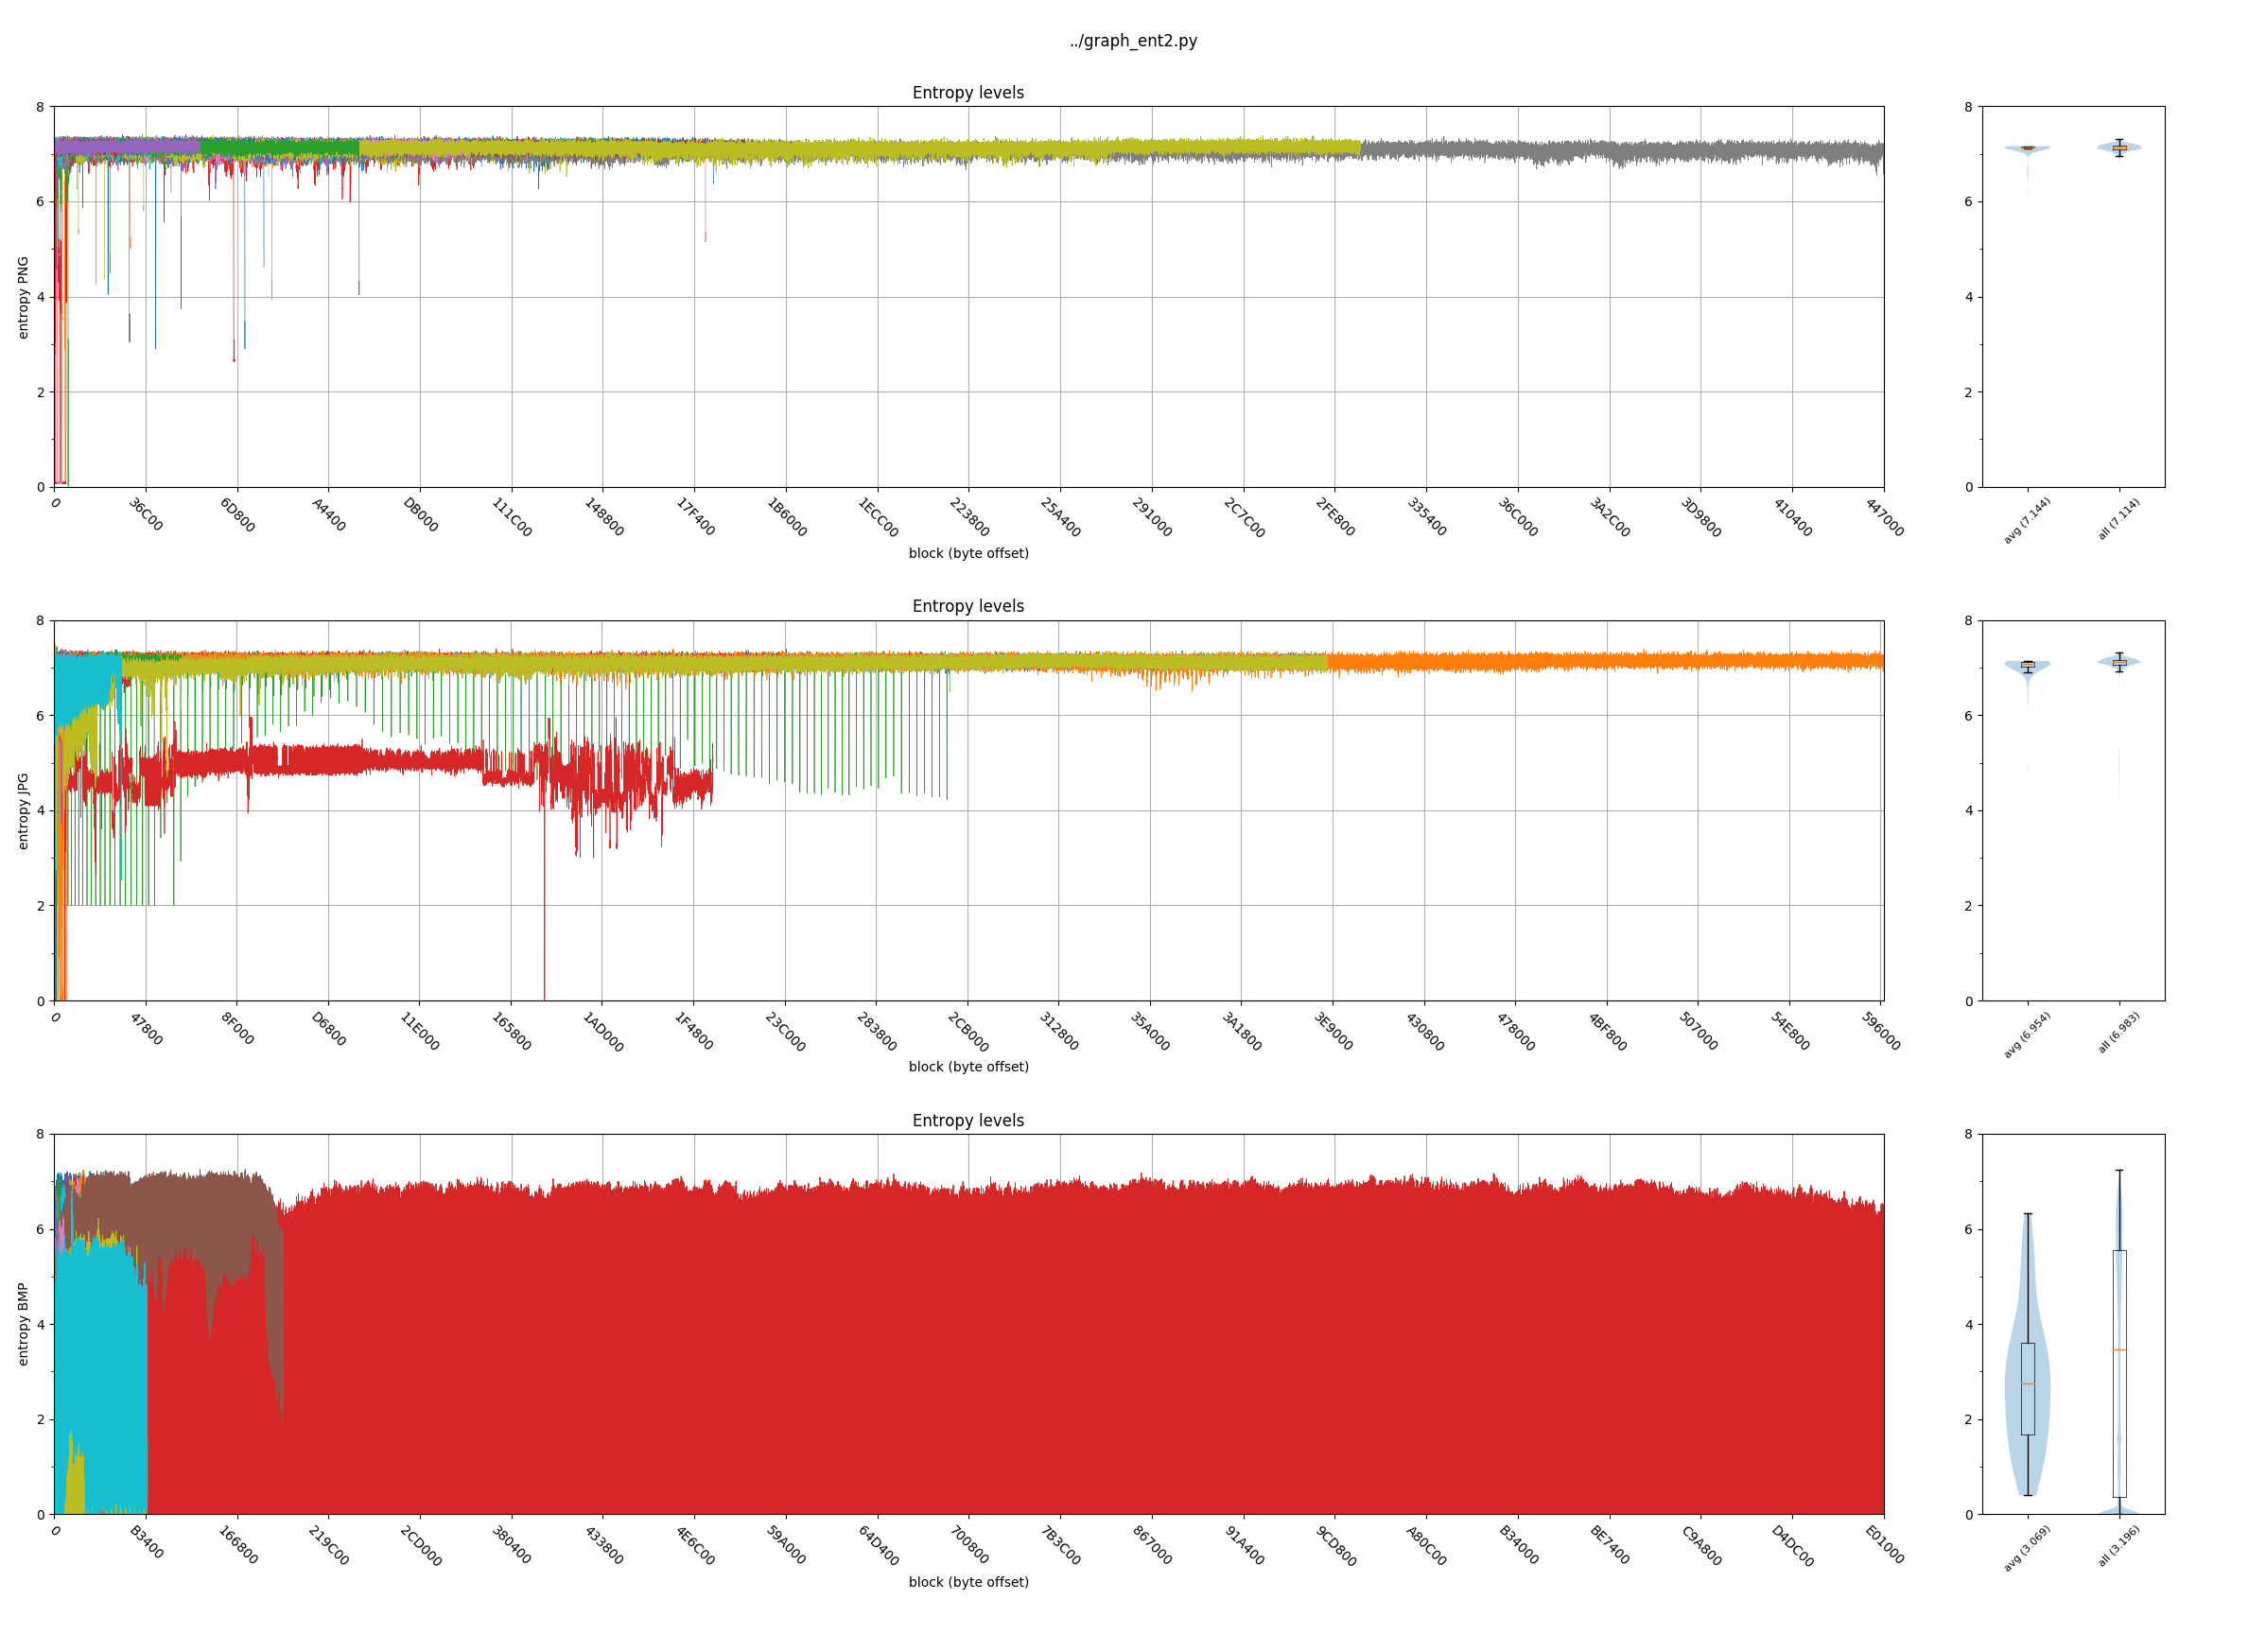
\includegraphics[width=\textwidth]{inc/statanalysis_graph}
	\caption{Distribution Analysis of Different, Common Graphics Formats}
	\label{fig:statGraph}
\end{figure*}

\begin{figure*}[ht]
	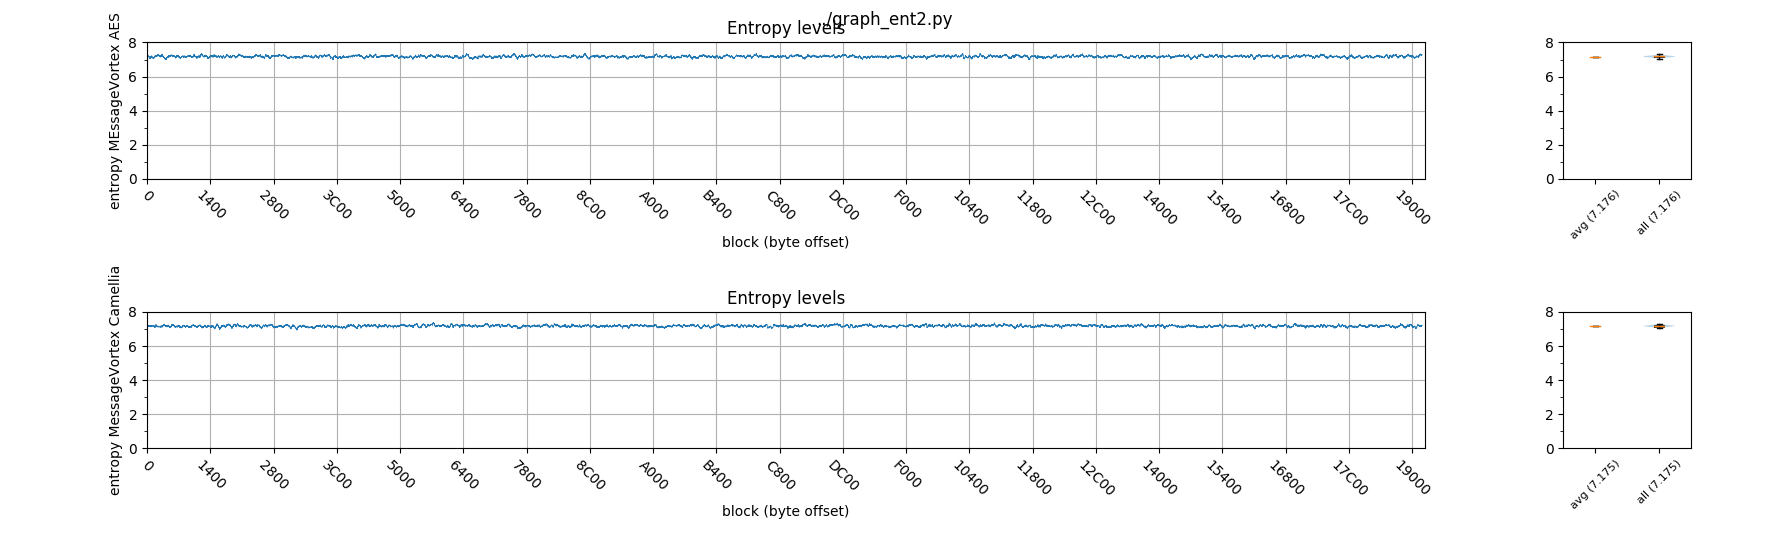
\includegraphics[width=\textwidth]{inc/statanalysis_mv}
	\caption{Distribution Analysis of a MessageVortex Block}
	\label{fig:statMvGraph}
\end{figure*}

We then carried out an analysis identifying the typical entropy and the inner structures. The graphs in \cref{fig:statGraph} show a typical analysis. In that case, we looked at 100 images of each type. We graphed and analyzed their entropy and tested for the suitability of a plain embedding from an entropy poi. Table~\ref{tab:fileEntropy} lists the average entropy of analyzed file types and makes remarks about the suitability for plain embedding. In practice, we found that most suitable file formats have an entropy of $\approx 7.2$ and an interquartile range (IQR) of 0.15 or less. Furthermore, files should have a big, uniform, non-structured range containing these characteristics. Such a file has a suitable space for embedding. For reference, \cref{fig:statMvGraph} shows the distribution of typical MessageVortex blocks. We did find that the entropy must be uniformly matched in the case of plain embedding.

\begin{table*}[!ht]
	\centering\tiny
	\begin{tabular}{|l|l|l|l|}\hline
		\diaghead{\theadfont Type Criteria}{Type}{Criteria} & \thead{Avg. Entropy}     & \thead{IQR} & \thead{Remarks}\\\hline
		JPG       & 7.008  & 0.097 & -- \\              
		PNG       & 7.116  & 0.086 & -- \\              
		GIF       & 6.978  & 0.194 & -- \\              
		BMP       & 2.997  & 4.964 & not suitable \\              
		PDF       & 6.660  & 0.282 & Hard to embed due to a very complex inner structure but well suited \\\hline              
		MP3       & 7.076  & 0.091 & -- \\              
		WAV       & 4.777  & 0.927 & -- \\              
		OGG       & 7.104  & 0.093 & relatively easy to embedd. Hard not to break the file structure. \\\hline              
		mpg4      & n/a    & n/a   & good to embedd. Steganography could be applied here easily too. \\\hline              
		zip       & 7.148  & 0.080 & easy to embedd when using ``password protected''  archives \\\hline\hline
		MVaes     & 7.176  & 0.072 & Without length padding as reference encrypted with AES 256 CBC\\
		MVcam     & 7.175  & 0.070 & Without length padding as reference encrypted with Camellia 256 CBC\\\hline
	\end{tabular}    
	\caption{comparison of protocols in terms of the suitability criteria as transport layer}
	\label{tab:fileEntropy}
\end{table*}

When blending into images, BMP showed a strongly varying entropy within a file. A sampling of ten blocks at random position resulted already in detection with a false positive rate below 5\%. PNG and JPG files showed to be very robust within the sample. We did not succeed in identifying the MessageVortex blending content based on entropy values. GIF images showed to be unsuitable. Archive formats such as zip files were extremely robust. We were able to embed it into a zip file and marking it (generically) as an encrypted file. This embedding was genuinely undetectable. However, such embedding may potentially lead to censorship based on the blacklisting of encrypted zip files.

OGG and MP3 are suitable. However, we were able to detect the entropy difference when taking extreme dense samples. These formats may, however, be suitable for not yet standardized forms of steganography. While PDF has low entropy and a high IQR typically, some parts of the files are very well suited for embedding. Plain embedding with knowledge of the format was even possible without affecting the visual result of the file.

We could show that with an approach based on Shannon entropy, we may identify plain embedded \VortexMessages in BMP and WAV files. 

All movie formats were performing similarly to jpg and PNG. However, due to the very complex structure with scattered blocks, they seem to be unsuitable for plain embedding. They are, however, strong candidates for steganography and are being used.

\section{Analysis of Routing Layer}
\subsection{Analysis of Core Operations}
The core operations form a toolset for mixing messages. Under the operational restrictions outlined in \cref{sec:routingStrategies}, we analyze in the following section the operations and determine their capability for leaking information or affecting security.

\subsubsection{Splitting and Merging}
The operations $splitPayload$ and $mergePayload$ are the trivial operations of our operations set. The operations by itself leak some information under the assumption that they were encrypted previously. A split or merge operation on its own leaks possible counterparts as the size should add up to a blocksize common in symmetric cryptography. As we outlined in \cref{sec:mergeAndSplit} and \cref{sec:routingStrategies} either an encryption step or an add redundancy step has to be added before a \VortexNode{} may forward the block to the next layer. When doing so, we can say that the operation leaks not more than any cryptographically secure operation.

For a \VortexNode{} executing the operation, a split operation does not leak any additional properties. The input may be payload or not. Therefore, the output of the operation has the same properties as the input. Unless the \VortexNodes{} knows the nature of the incoming payload, the output may be either decoy or true message traffic.

\subsubsection{Encryption and Decryption Operations}
All encryption steps do leak some properties. They may leak the algorithm due to the block size. The chosen parameter may be unique to the RBB. If randomly chosen, this is no longer the case. If chosen by an implementation-specific pattern, the pattern may leak the implementation over time. As the analysis must be done over a short period of time (the lifetime of an \defref{eID}), it is up to an RBB to leak as little information as possible. We do regard the cryptographically secured content as secure. 

\subsubsection{Add and Remove Redundancy Operations}\label{sec:analysisReedSolomon}
During analysis, the $addRedundancy$ operation showed the undesirable behavior that applying the operation lowered the entropy of the target blocks, as shown in \cref{fig:entropy}. 

We did reconsider thus the whole operation. The choice of the Reed-Solomon (RS) operation instead of a Lagrange polynomial seemed logical. As the possibilities to recover from cheaters in an RS setting of varying contexts, have already been studied in \cite{mceliece1981sharing}, \cite{bu2017rasss}, and similar publications.

%%%%%%%%%%%%%%%%%%%%%%%%%%%%%%%
%%% Preplaced float
%%%%%%%%%%%%%%%%%%%%%%%%%%%%%%%
\begin{figure*}[!t]\centering
	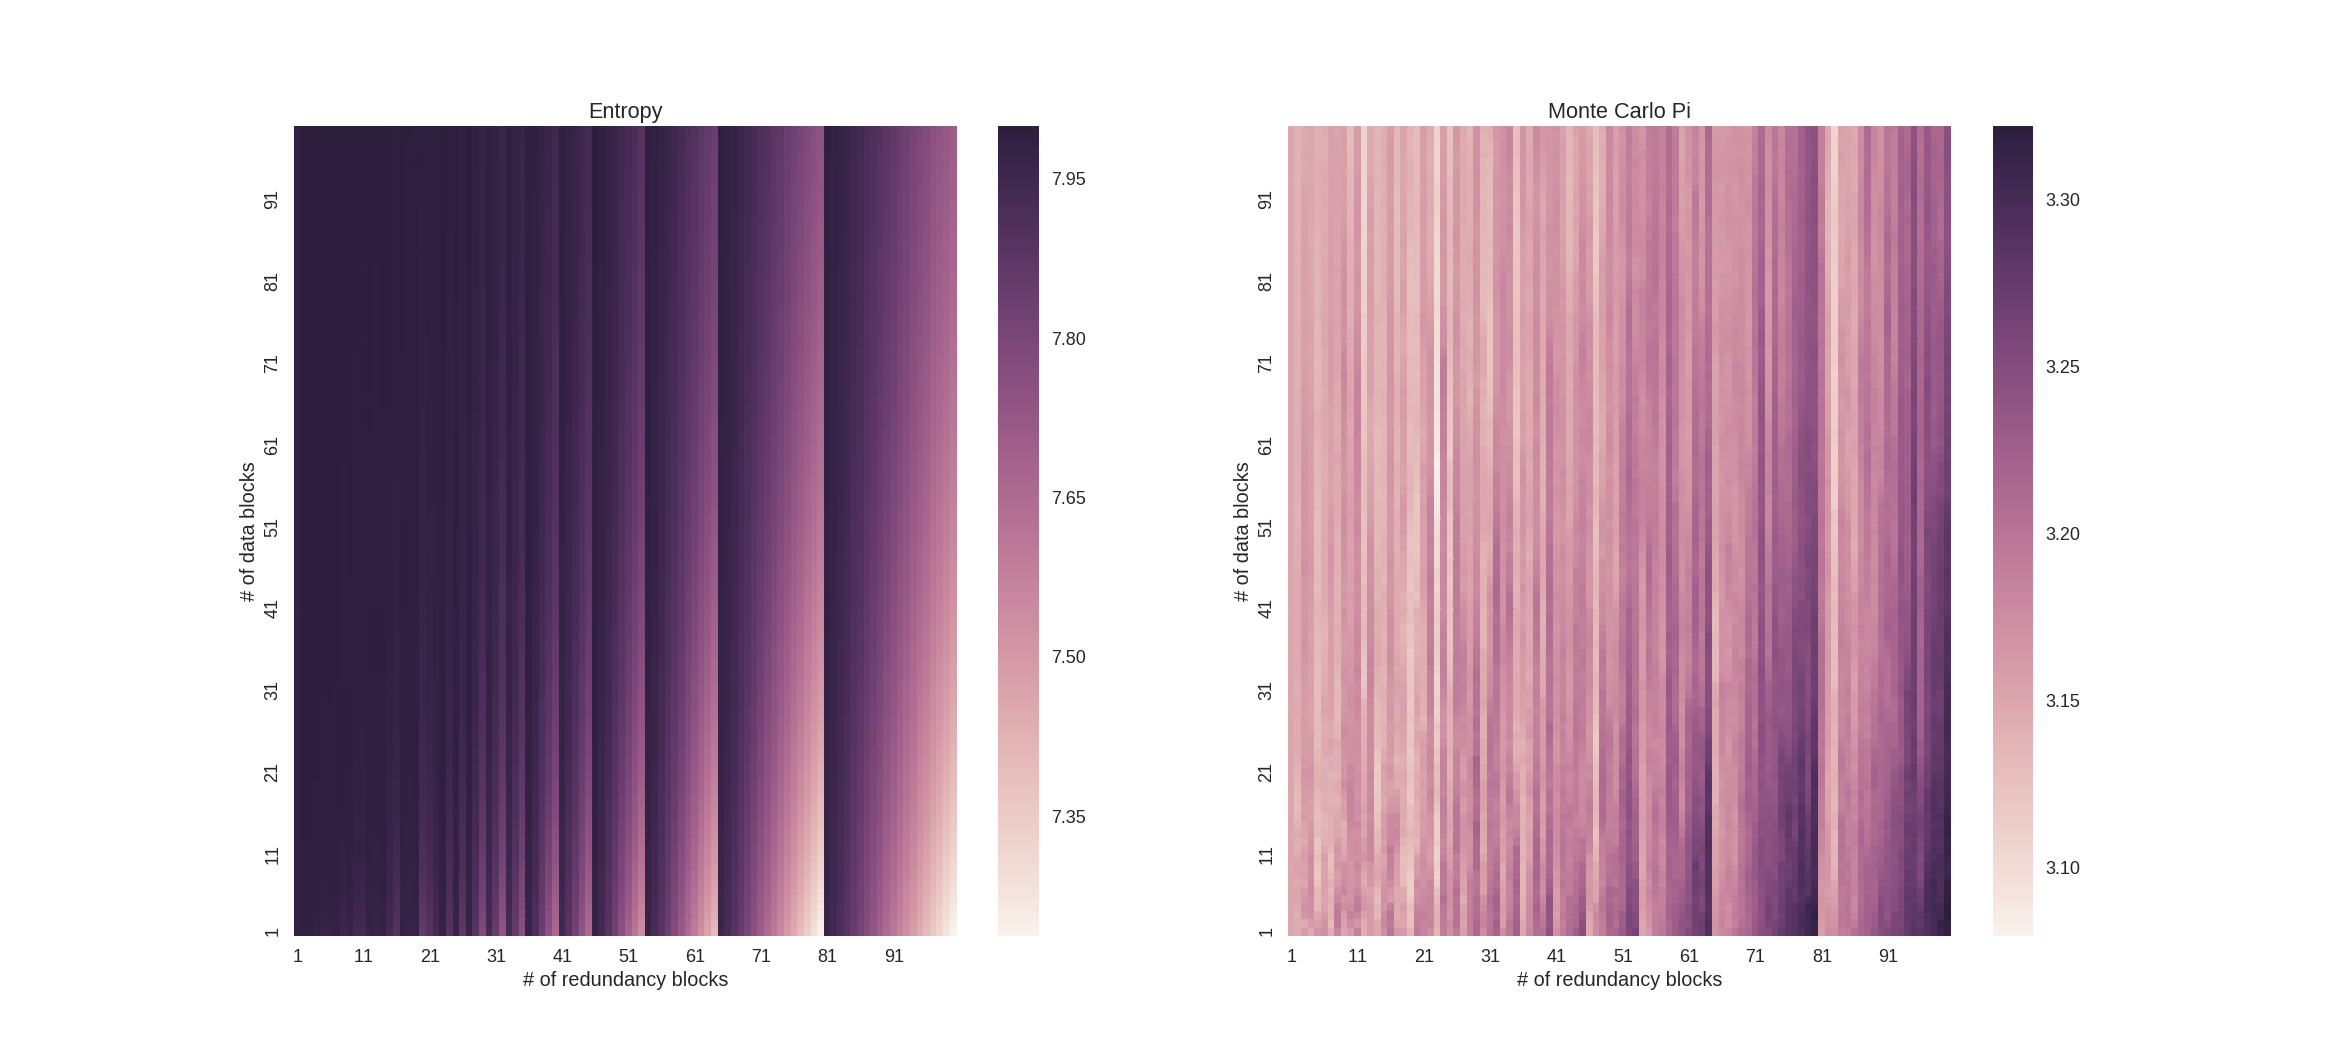
\includegraphics[width=1\textwidth]{inc/randomblock_10kb}
	\caption{Resulting entropy of addRedundancy with and without encryption step}
	\label{fig:entropy}
\end{figure*}


\section{Senders routing layer}
A sender may have some knowledge about the Routing block size and may, therefore, guess the complexity of the routing path. He is, however, unable to gain any additional information such as time of travel or number of hops until the target.

\section{Intermediate node routing layer}
An intermediate node does know all the operations applied and the immediate next hop. It does learn the routing addresses of the immediately following endpoints but is unable to use these endpoints. This is because he has no means to get the host key required to communicate.

If a routing block is repeated, a router may identify the routing block as repetition. Identifying the repetition of a block can be done by looking at the serial number of replay protection. We then may give a rough estimate of the message size by comparing the payload chunks. This estimate is, however, very rough as it is bounded by the block size of the symmetrically applied encryption.

\section{Security of Protocol Blocks}
To analyze the security of the protocol, we first go through all protocol blocks. After that, we will look at the possibilities of block recombinations and how to gain data or services based on such behavior. 

Assuming plain embedding, the presence of a chain of blocks may leak an existing VortexMessage. At the moment, the protocol expects at the offset and the size of the bytes to be skipped to the next block. The encoding does not assume an end of the chain marker as such a marker would make the design identifiable. As an encoding scheme, a variable byte length has been chosen. This guarantees that any file will always result in a valid chain of blocks and thus not leak such a presence.

The entropy of the only two blocks in this stream (MPREFIX and InnerMessageBlock) is comparable as both blocks are encrypted. Both blocks are encrypted and feature a similar entropy. The blocks follow each other without any delimiter. This results in a continuous stream of data with constant properties. 

To avoid repeating patterns at the beginning of streams due to reused identity blocks, a MURB must provide sufficient peer keys and prefix blocks. A VortexNode may, however, refuse to process MURBS (only accept maxReplays equal to 0).

All blocks of InnerMessageBlock are protected by the peer key $E^{K_{peer}}$. The forward secrets in all blocks except the payload blocks make sure that the recombination of blocks does not work for an adversary. To be successful, an adversary requires to know the forward secret of the next hop.

To keep the secrets of the next hop hidden from the host assembling the message, the subsequent header and the routing block are protected by the sender key $E^{K_{sender}}$. A message assembling node is, therefore, not even capable of creating its own messages to an unknown node as the hosts' public key $E^{K^{1}_{host}}$ is not derivable from a message.

Therefore, a routing node is not able to assemble messages for a specific host on the base of a routed message only. A routing node does not gain any additional knowledge except for the locally executed operations, the number of messages of the ephemeral identity, the size of messages of any ephemeral identity, the sending IP of a received \VortexMessage, and the transport endpoint address of any receiving endpoint. The most critical information is endpoint data, as all other data is unrelated to the original message (sender recipient and size). This information becomes absolutely crucial if assuming a censoring adversary. Therefore, a sender in a jurisdiction where the use of MessageVortex is deemed illegal must use only trusted nodes within the jurisdiction and at least for the first hop outside the jurisdictional reach of an adversary.


\chapter{Dynamic Attack Analysis}\label{sec:dynamicAnalysis}
In the dynamic analysis, we reach out to an active adversary. An active adversary modifies traffic in a non-protocol conformant way or misuses available or obtained information to disrupt messages, nodes, or the system as a whole.

\section{Well Known Attacks}\label{sec:wellKnownAttacks}
In the following sections, we emphasize on possible attacks to anonymity preserving protocols. Such attacks may be used to attack the anonymity of any entity involved in the message channel. In a later stage, we test the protocol for immunity against these classes of attacks.

\subsection{Broken Encryption Algorithms}
Encryption algorithms may become broken at any time. Our protocol is especially susceptible to this as it offers no perfect forward secrecy (PFS) on the transport layer. This either to new findings in attacking them, by more resources being available to an adversary, or by new technologies allowing new kinds of attacks. A proper protocol must be able to react to such threads promptly. This reaction should not rely on a required update of the infrastructure. Users should solely control the grade of security. 

We cannot do a lot for attacks of this kind to happen. However, we might introduce a choice of algorithms, paddings, modes, and key sizes to give the user a choice in the degree of security he wants to have.

We have introduced a way to support a set of independent cryptographic algorithms, paddings, modes, and prngs. The support of these algorithms does not have to be uniform throughout the system. Instead, it is sufficient for two neighboring nodes to support the same algorithms in order to be used. 

Another way of minimizing the impact of reduced security of encryption algorithms is to use long host keys. If an algorithm's security is only reduced by a couple of bits instead of being broken, a long key minimizes the impact and ay buy some time to switch to an alternate algorithm. 

A broken algorithm is severe if it leads to the decryption of the final messages to the recipient node. In such a case, an adversary would be able to rebuild the content of a workspace and thus effectively enable the adversary to obtain the content of the message.

\subsection{Attacks Targeting Anonymity}
Attacks targeting users anonymity are the main focus of this work. Many pieces of information may be leaked, and the primary goal should, therefore, rely on the principles established in security.

\begin{itemize}
	\item Prevent an attack\\
 	      Attack prevention can only be done for attacks that are already known and may not be realistic in all cases. In our protocol, we have strict boundaries defined. A node under attack should at any time of protocol usage (this excepts bandwidth depletion attacks) be able to block malicious identities. Since establishing new identities is costly for an attacker, he should always require far more resources than the defender.
	\item Minimize attack surface\\
	      This part of the attack prevention is included by design in the protocol. By minimizing the information footprint, we have in each operation and the disconnection between two \defref{eID}s of the same sender, it is very hard to gain additional information based on statistical means.
	\item Redirect an attack\\
	      Although the implementation does not do this, it is possible to handle suspected malicious \VortexNode{} differently (e.g., avoid using them or only use them for decoy traffic, not disclosing identities).
	\item Control damage\\
	      For us, this means leaving as little information about identities or meta information as possible on untrusted infrastructures. If we leave traces (i.e., message flows or accounting information), they should have the least possible information content and should expire within a reasonable amount of time.
	\item Discover an attack\\
	      The protocol is designed in such a way that attack discovery (such as a query attack) is possible. However, we consider active attacks just as part of the regular message flow. The protocol must mitigate such attacks by design.
	\item Recover from an attack\\
	      An attack does always impose a load onto a system's resources, regardless of its success. It is vital that a system recovers almost immediately from an attack and is not covered in a non-functional or only partial-functional state either temporarily or permanently.
\end{itemize}

In the following subsections, we list a couple of attack classes that have been used against systems listed in \cref{sec:implSystems} or the respective academic works. We list the countermeasures which have been taken to deflect these attacks.

\subsubsection{Probing Attacks}
Identifying a node by probing and check their reaction is commonly done when fingerprinting a service. As a node is participating in a network and relaying messages probing may not be evaded. However, it may be made costly for an adversary to do systematic probing. This should be taken into account. Both currently specified transport protocol features an indefinite number of possible accounts. Since not the server but the endpoint address is behaving, node probing is more complicated than in other cases where probing of service is sufficient. 

One of the problems is clear-text requests. These requests may be used on any transport layer account without previous knowledge of any host key. Thus the recommendation in \cref{tab:protoReplyCrit} is generally not to answer the requests. Routing nodes in jurisdictions not fearing legal repression or prosecution may reply to clear text requests, but it is usually discouraged as they allow harvesting of \VortexNodes{}. A discovered \VortexNode{} may leak subsequent nodes if the same account is used for receiving and sending.

One strategy to avoid would be to put high costs onto clear-text requests in such a way that a clear-text request may have a long reply time (e.g., up to one day). 

A node is free to blacklist an identity in case of an early reply. This is an insufficient strategy as a big adversary may have lots of identities in stock. Requesting an unusually long key as a plaintext identity does not make sense either as these as well may be kept in stock. We may, however, force a plaintext request to have an identity block with a hash following specific rules. We may, for example, put in a requirement that the first four bytes of the hash of a header block correspond to the first four characters of the routing block. At the moment, this has been rejected in the standard for practical reasons. First, as the request is unsolicited, a sender is the only one able to decide the algorithm of the hash. This would allow a requester to choose upon the complexity of the puzzle. Second, any negotiation of the cost of the request would result in the disclosure of the node as \VortexNode, which might be unsuitable.

\subsubsection{Hotspot Attacks}
Hotspot attacks aim to isolate high traffic sites within a network. By analyzing specific properties or the general throughput locations with outstanding traffic may be identified. These messages do quite often reveal senders or recipients. Sometimes an intermediate node in an anonymizing system. 

The assumption that a hotspot arrises at a specific point in our protocol is wrong, as at any point, either payload blocks are left out until expiry or additional traffic may be generated using an $addRedundancy$ operation.

\subsubsection{Message Tagging and Tracing}
When using an anonymization system, a message may be either fully or partially traced or even tagged. Tagging allows one to recognize a message at a later stage and map it to its predecessors. Protocols with tagable messages are not suitable for anonymization systems.

\VortexMessages{} are not tagable. The constraint ``no repeating pattern'' prohibits forwarding of any block without an appropriate operation. This denies the possibility of tagging a payload block. All other blocks (prefixes, header, and routing block) are discarded when forwarding the message. The same applies to the carrier message, which is used as transport for the blended \VortexMessage.

Injecting a value into a payload block and following it would imply that the evil \VortexNode{} has knowledge about all subsequent operations and keys, which is equivalent to know the subsequent private keys of the \VortexNodes. We will cover this scenario in \cref{sec:analysisInteractionGraphs}.

\subsubsection{Side Channel Attacks}
Side-channel attacks are numerous. Especially important to us are attacks related to either lookup in independent channels (e.g., downloading of auxiliary content of a message) or behavior related to timing patterns.

\subsubsection{Sizing Attacks}
There are two kinds of sizing attacks identified to be relevant for us. One is the possibility for matching messages with related sizes, and the other one is to relate message size to the original messages. Both attacks may be considered as a tracing attack and will be analyzed accordingly. 

When matching messages in size, an attack is attractive if it allows collapsing the operations of one or multiple honest \VortexNodes{} between two malicious \VortexNodes. To do so, the second evil node may match the sizes of the received payload blocks and hypothesize about which blocks are equal, or it may assign the \defref{eID} of the first evil node to the \defref{eID} of the second node. The matching is not trivial, as\ldots

\begin{enumerate}
	\item The sizes are likely to have changed while transferred through the honest nodes.
	\item The number of payload blocks may have changed.
	\item The size may have been further obfuscated by the fact that an onionized encryption does either not add to the size (if an algorithm with the same block size is applied and no padding) or is increasing (by the block size). Obfuscation is possible as well, if we apply a $splitPayload$ or $mergePayload$ operation with a subsequent encryption (mandatory to not violate the ``repeating pattern rule'') or an $addRedundancy$ operation.
\end{enumerate}

\subsubsection{Bugging Attacks}
Numerous attacks are available through the bugging of a protocol. In this chapter, we outline some of the possibilities and how they may be countered:

\begin{itemize}
	\item Bugging through certificate or identity lookup:\\
	Almost all kinds of proof of identities, such as certificates, offer some revocation facility. While this is a perfect desirable property of these infrastructures, they offer a flaw. Since the location of this revocation information is typically embedded in the proof of identity, an evil attacker might use a falsified proof of identity with a recording revocation point.
	
	There are multiple possibilities to counter such an attack. The easiest one is to do no verification at all. Having no verification is, however, not desirable from the security point of view. Another possibility is only to verify trusted proof of identities. By doing so, the only attacker could be someone having access to a trusted source of proof of identities. A third possibility is to relay the request to another host either by using an anonymity structure such as Tor or by using its infrastructure. Using Tor would violate the ``Zero Trust'' goal. Such a measure would only conceal the source of the verification. It would not hide the fact that the message is processed. A fourth and most promising technology would be to force the sender of the certificate to include a ``proof of non-revocation''. Such proof could be a timestamped and signed partial CRL. It would allow a node to verify the validity of a certificate without being forced to disclose itself by doing a verification. On the downside has to be mentioned that including proof of non-revocation involves the requirement to accept a certain amount of caching time to be accepted. This allowed caching time reduces the value of the proof as it may be expired in the meantime. It is recommended to keep the maximum cache time as low as 1d to avoid that revoked certificates may be used. 
	
	\item Bugging through DNS traffic:\\
	A standard protocol on the Internet is DNS. Almost all network-related programs use it without thinking. Typically the use of such protocol is only a minor issue since the resolution of a lookup is usually made by an ISP. In the case of a small Internet service provider (ISP), this might, however, already become a problem.
	
	The bugging in general attack works as follows: We include a unique DNS name to be resolved by a recipient. This can be done most easily by adding an external resource such as an image. A recipient will process this resource and might, therefore, deliver information about the frequency of reading or the type of client. 
	
	It must be taken into account that the transport layer will always do DNS lookups and that we may not avoid this attack completely. We may, however, minimize the possibilities of this attack.
	
	\item Bugging through external resources:\\
	A straightforward attack is always to include external resources into a message and wait until they are fetched. In order to avoid this kind of attack, plain text or other self-contained formats should be used when sending a message. As we may not govern the type of contained message, we can make at least recommendations concerning its structure.
\end{itemize}

\subsubsection{Analysis by Building Interaction Graphs\label{sec:analysisInteractionGraphs}}
Building interaction graphs is very hard with our system. Although we cannot quantize the effect, we still may elaborate on the difficulties. We first look at our system from an outside view and then do the same for a powerful adversary inside the system.

When looking from outside the system, interaction graphs are hard to build as sending and receiving transport addresses and protocols do not match, which adds tremendously to the complexity. An outside observer may not just observe a specific SMTP server. He must track incoming messages, observe the user (typically obtaining the mail by IMAP) fetching the messages, and then follow all possible connections to other infrastructures known to be supported and suspect them as outbound messages. By assuming that an outside observer is able to identify all \VortexMessages{} and surpass all difficulties involved in following the different protocols. Then such an observer is capable of generating a graph having as nodes all \VortexNodes{} and as edges all \VortexMessages{}. An adversary would then require the means to identify the sender and recipient. We first claim that there is no possibility to identify such senders and recipients as there is no guaranteed minimum or maximum time for a message. As an immediate result, any \VortexNode{} sending a message may be a sender of a message or only a router. Inversely, any \VortexNode{} receiving a message may be either a recipient or a router. Due to the operations, sizes may increase or decrease on message paths. Therefore, an outside adversary is unable to match two adjacent messages to the same identity. Any previous message, including all subsequent messages, may have triggered the sending of the message. So from an outside perspective, we have no possibility to identify by message pattern, message size, or message sequence adjacent messages.

We assume the example routing graph, as shown in \cref{fig:messageGraphPaths}.

\begin{figure*}[!t]\centering
	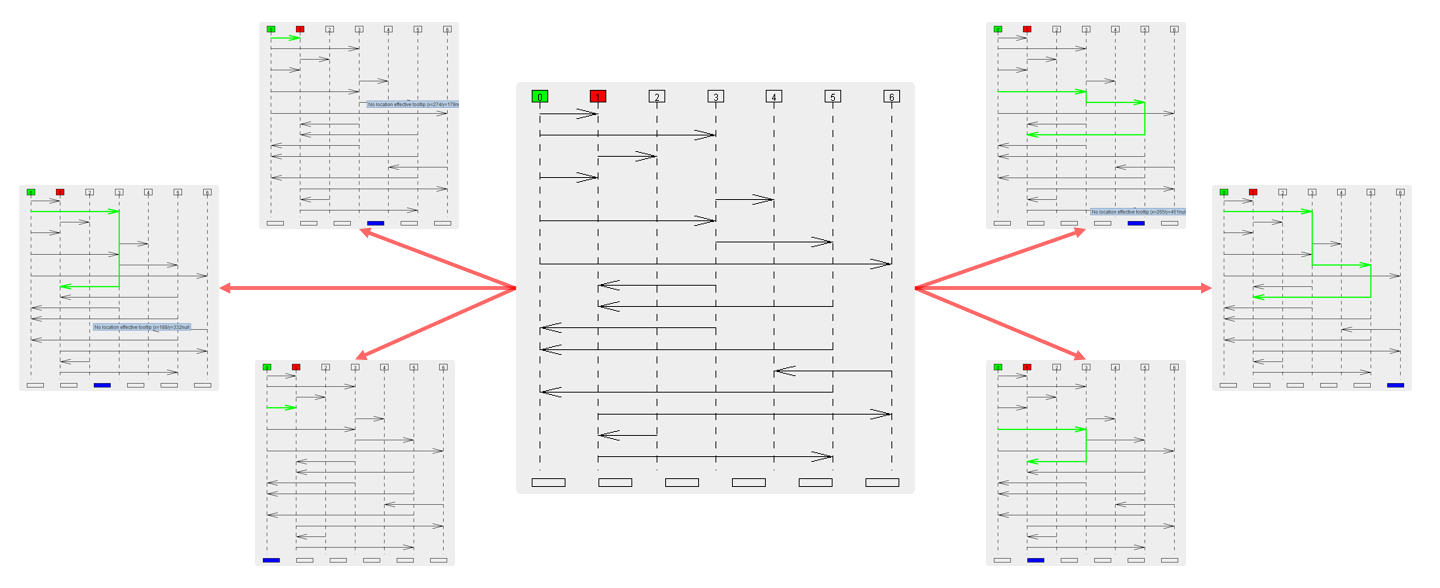
\includegraphics[width=1\textwidth]{inc/messageGraphPaths}
	\caption{A randomly generated graph with highlighted paths to the target.}
	\label{fig:messageGraphPaths}
\end{figure*}


From an inside perspective, we may take additional information into account. First, if an adversary has control over a routing node, he is aware of all operations carried out by this node. He knows the immediate sender and the immediate recipient of any immediately subsequent messages. If the adversary has control over two or more adjacent \VortexNodes{}, he is able to collapse the operations into one big workspace with the combined operations, whereas the message transfer may be reflected in a simple mapping operation. He is also able to identify subsequent messages using the same \defref{eID}s as messages of the same RBB. He is, however, unable to tell whether or not two subsequent incoming \VortexMessages{} for the same \defref{eID} belong to the same or to two different messages. If the same RBB maintains multiple \defref{eID}s simultaneously on the same routing node, the node is unable to match those \defref{eID}s to the same RBB as they share no common properties. In a worst-case scenario, this means that all routing nodes chosen by the RBB, with the exception of the sender node and the final recipient node,  are under the control of an adversary. This would effectively collapse an interaction graph to a reduced graph, as shown in \cref{fig:reducedMessageGraphPaths}. An adversary learns that there are two adjacent nodes to his network (node 0 and 1). Such an adversary is, however, unable to tell whether node 0 was an initial sender, as any incoming message into node 0, regardless of its source or timing, may have been the cause for the original message sending. Arguing the same way, we may say that either node 0 or 1 cannot be the recipient for sure as any other outgoing message, regardless of timing or size, may have been triggered by the incoming target, and the final recipient may be any subsequent node.

\begin{figure*}[!t]\centering
	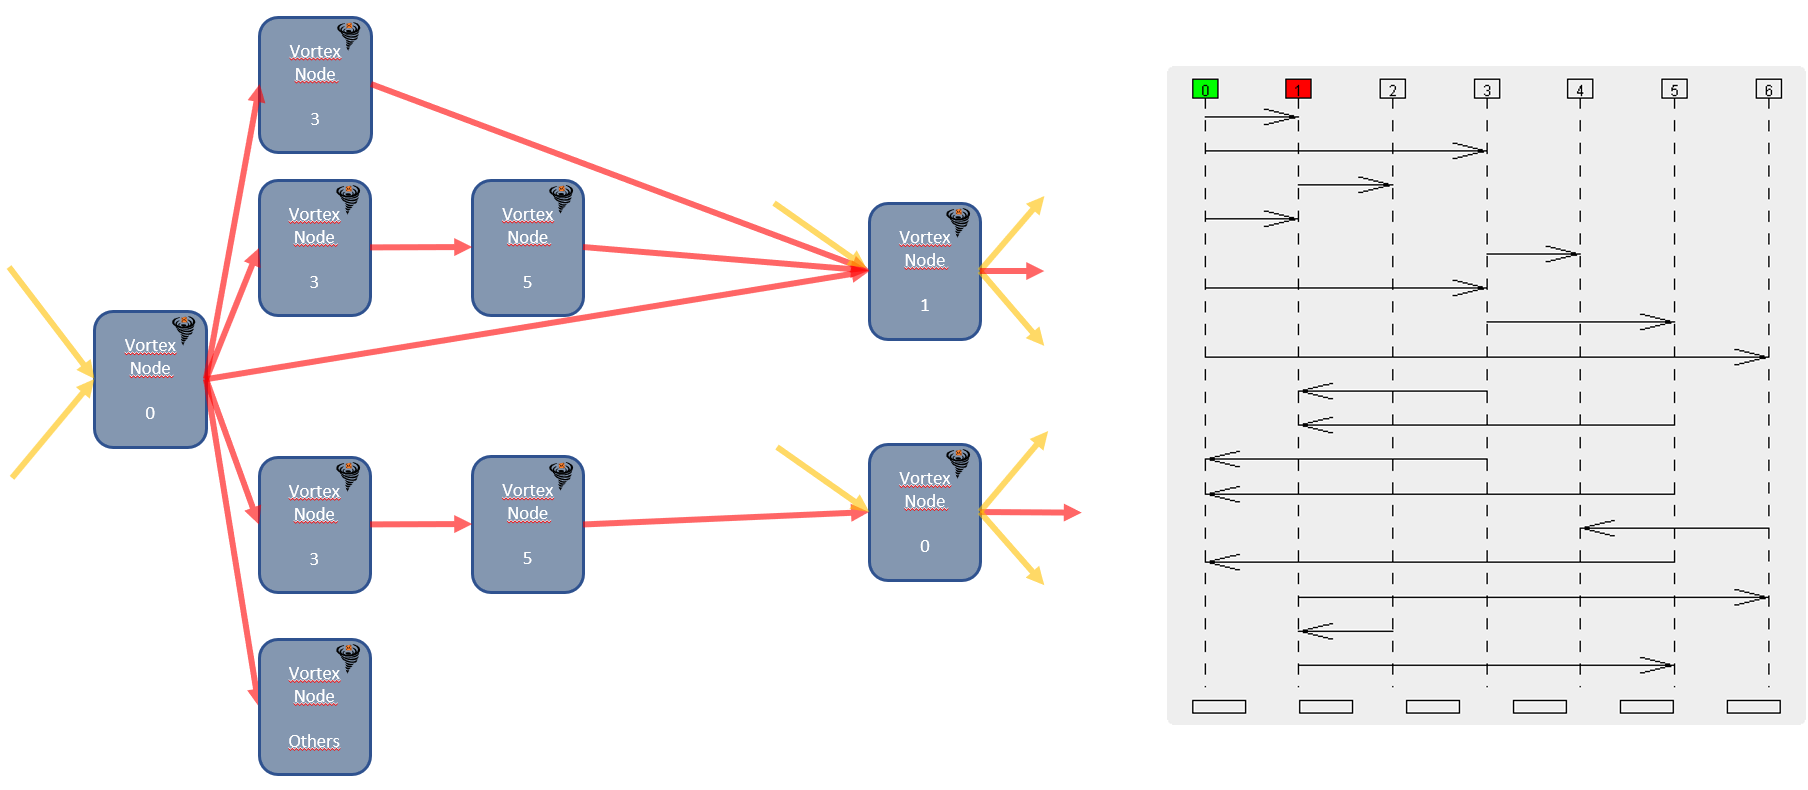
\includegraphics[width=1\textwidth]{inc/reducedMessageGraphPaths}
	\caption{A randomly generated graph assuming that all nodes except node 0 and 1 are collaborating.}
	\label{fig:reducedMessageGraphPaths}
\end{figure*}

We, therefore, can tell that we do need trust in the sending and receiving node to be safe. Furthermore, we need additional traffic generated by any non-collaborating \VortexNode{}. The fact that there are neither timing nor sizing constraints makes it impossible to match any two messages to the same original sender. Therefore, our message is not traceable if there is additional traffic going through our trusted nodes, and honesty of the initially sending node as well as the final recipient node is assumed.

\subsection{Denial of Service Attacks}
\subsubsection{Censorship}
Whereas traditional censorship is widely regarded as selective information filtering and alteration, very repressive censorship can even include denial of information flows in general. Any anonymity system not offering the possibility to hide in legitimate information flows, therefore not censorship-resistant.

\subsubsection{Denial of service}
An adversary may flood the system in two ways.
\begin{itemize}
	\item He may flood the transport layer exhausting resources of the transport system.\\
	This is a straightforward attack. MessageVortex has no control over the existing transport protocol. Therefore, all flooding attacks on that layer are still effective. However, If an adversary attacks a node, the redundancy of a message may still be sufficient. On the other hand, flooding disrupts at least all other services using the same transport layer on that node. This result may be unacceptable for an attacker. More likely would be censorship.
	\item He may flood the routing layer with invalid messages.\\ 
	Identifying the messages is relatively easy for a node. Usually, it should be sufficient to decode the CPREFIX block of a message. If the CPREFIX is valid, then the header block either identifies a valid identity or processing may be aborted. 
	\item He may flood an accounting layer with newIdentity.\\
	Flooding an accounting layer with identities is possible. Since the accounting layer is capable of adapting costs to a new identity, it may counter this attack by giving large puzzles to new identities. This affects all new identities and not only those flooding. If a flooding attack is carried out over a long time, a node may decide to split its identity. All recent active users get a new identity, whereas the old one opposes high costs. This would force an attacker to work in intervals and is no longer able to make a permanent DoS attack.
\end{itemize}

\subsubsection{Credibility Attack}
Another type of DoS attack is the credibility attack. While not a technical attack, it is very effective. A system not having a sufficiently big user base is offering thus a lousy level of anonymity because the anonymity set is too small or the traffic concealing message flow is insufficient. 

Another way is to attack the reputation of a system in such a way that the system is no longer used. An adversary has many options to achieve such a reduction in credibility. Examples:
\begin{itemize}
	\item Disrupt functionality of a system.\\ 
	This may be done by blocking the messaging protocol it uses or by blocking messages. Furthermore, an adversary reduces functionality when removing known participants from the network either by law or by threatening.
	\item Publicly dispute the effectiveness of a system.\\
	Disputing the effectiveness is a very effective way to destroy a system. People are not willing to use a system which believed to be compromised if the primary goal of using the system is avoiding being observed.
	\item Reduce the effectiveness of a system.\\
	A system may be considerably loaded by an adversary to decrease the positive reception of the system. He may further use the system to send \defref{UBM} to reduce the overall experience when using the system. Another way of reducing effectiveness is to misuse the system for evil purposes such as blackmailing and making them public.
	\item Dispute the credibility of the system founders.\\
	Another way of reducing the credibility of a system is to undermine its creators. If -- for example -- people believe that a founders' interest was to create a honey pot (e.g., because he is working for a potential state-sponsored adversary) for personal secrets, they will not be willing to use it.
	\item Dispute the credibility of the infrastructure.\\
	If the infrastructure is known or suspected to be run by a potential adversary, people's willingness to believe in such a system is expected to be drastically reduced.
\end{itemize}

\subsubsection{Denial of Service by Exhausting Quotas or Limits}
A malicious node may try to exhaust quotas or limits. As we do trust in the sender and recipient, all other nodes do not know the forward secrets used in the message. The options for an adversary are then as follows:

\begin{itemize}
	\item Resend a MURB (with different content) as often as possible to exhaust message and transfer quota. 
	\item Create intentionally huge, incorrect message content to exhaust transfer quota.
\end{itemize}

\subsection{Attacking Sending and Receiving Identities of the MessageVortex System}
The most valuable goal of an adversary is breaking an entity's anonymity or monitor their traffic by the content or the metadata. In the following sections, we analyze the possibility of determining the sender or recipient of a message.


\subsubsection{Traffic Highlighting}
Traffic caused by a routing block may be observed to a certain extent on a statistical basis. A node may generate bad message content of exceptionally large or small nature. This might potentially highlight messages involved in message routing using no split or relative split operations as well as addRedundancy operations.

\subsection{Recovery of Previously Carried Out Operations}
It is crucial that an adversary is unable to recover parameters of a previously carried out operation. We analyzed the protocol operations carefully to be sure not to leak any of the parameters. Some operations leak apparent data, such as an encryption operation with a block cipher does typically leaks its block size. This has, however, been classified as invaluable data as the block size does not result in any information gain usable for attacking the system or narrowing down efforts. In \cref{fig:entropy}, we can show that the parameters are visible. We took the same 10kb block and treated it with all possible combinations of operation parameters. The image shows that there is a possibility of guessing the parameter with a high probability. For guessing the average Monte Carlo Pi and the average Shanon entropy in bits per byte were already sufficient. The results got a bit less clear when applying the same operation to random blocks while doing the analysis. 

We have, however, found a flaw in the$addRedundancy$ operation. When applying this operation to an encrypted block, the entropy of the resulting block leaks some of the parameters of the operation. As a result of this finding, we added a custom padding and an additional encryption step. The repeated analysis showed that the operation does no longer leak these parameters through this channel.

\section{Side Channel Leaking}
We tried to minimize the number of possible side channels. Some of the side channels are irrelevant as they are controlled by trusted nodes. Some side channels remain unavoidable unless we restrict messages to an unrealistic minimum. 

\subsection{Software Updates and Related Data Streams}
We consider assuming in today's world that updates are not needed for security reasons a foolish thing. However, downloading a software update may uncover a user. While it is doable to transport software unseen once, doing it on a regular basis is a tedious job. We, therefore, included a standard way of querying a new software release and getting the new release over the \MessageVortex{} protocol allowing the same degree of privacy as with all other messages sent. While the path itself is cryptographically secured, we recommend that code should still be signed, and the signature should be verified prior to upgrading to a new software version.

\subsection{Bugging in transported messages}
Bugging in transported messages is possible as we have no clear definition of the content of a message. As the transport is currently XMPP and SMTP, the assumption of sending MIME-encoded messages is obvious. The availability of clients and the simple feasibility of gateways make it an obvious choice. If we use MIME as transport encoding, we may leak certain attributes such as the reading location of a message to a sender by including external images or signing the message with a certificate whose verification authority is tapped. Since we trust the sender and recipient node and assume that the RBB is one of them, this argument does not count towards any of the messages. Any other intermediate routing node has no means of injection any content into the message or the routing blocks. Therefore, in terms of bugging protocol messages, our protocol is rather secure.

This statement leaves some interesting aspects unanswered. First, when creating an \defref{eID} on an intermediate node, we have to analyze this situation as well as in such a situation, trust into the target node (the node on which an \defref{eID} is allocated) is most likely not trustworthy. While the node is a final node for the request, the node is not regarded as the final destination for a message. In that specific case, the reply block the node receives maps not to ID 0 but to but to ID 32767 (see \cref{tab:workspaceId}). This difference keeps a routing node to misuse the reply block for sending a bugged message.

\subsection{Exploiting MURBS}
Multi-Use Reply Blocks (\defref{MURB}s) are another source for a side-channel attack. While technically safe, the possibility of creating repeating patterns over a network causes the possibility to recognize the communication pattern. As we have no strict timing for sending our messages, this pattern discovery remains a not easy solvable problem. To make it even harder, we restricted the reuse of a MURB by design to 127 times and included the possibility to use different prefix blocks in each message. Without these prefix blocks, the pattern would have been easily identifiable as the prefix block would have formed a byte sequence that would have been detectable in all messages using the same MURB.

Replaying a message built with a MURB does not necessarily require to identify \VortexMessages{}. It is sufficient to store and replay a suspected message and trying to analyze whether a related communication pattern is visible. The pattern reflects all messages which are triggered by the message. As an adversary does not know whether he replayed the first or an intermediate message, he is unable to tell whether he was able to observe the full graph or just a subset. Furthermore, the graph generated by the replaying (assuming that the replay protection did not catch the message) may be smaller, as other parts of the message traveling through other nodes may not have been replied to, leading to non-sendable messages.

If we assume that an adversary identifies all messages and involved \VortexNodes{} of a MURB, we have two things to consider. In an environment of a censoring adversary, the confidentiality of \VortexNodes{} is compromised. Additionally, in an environment of an observing adversary with many MURBs, high replay ratios, and small routing sets, we would be able to build a list of the routing set an unknown \VortexNode{} has, leading to pseudonymity for that node. Right now, we are unable to see how this could be further exploited, but this fact should be mentioned. 

To weaken the threats of MURBs, we eradicated all needs for MURBs within the protocol. A MURB has only to be used when a user decides to do so, and we recommend not using them.

\section{Achieved Anonymity and Flaws}
\subsection{Measuring Anonymity}
It is tough to measure anonymity, as it involves many uncontrollable factors. We may, however, control the degree of anonymity according to the number of involved parties. Assuming a sender knows the complete message path, including all operations carried out on any untrusted node a message travels through, the anonymity is maxed to the number of involved nodes $n$, excluding the sender nodes. This degree of $n-1$ may be further reduced if all well-known ``routing only'' or at least ``routing mostly'' nodes are reduced. Under these harsh assumptions, the set may be reduced to the potential set of ``well known'' recipients of a message.

We have to differentiate between several problems. An adversary has to identify the participants of an anonymity system. Then he has to identify members of a message or a communication anonymity set. Starting from there, he has to identify message flows and detect senders and receivers of messages within an anonymity set (which is not doable in all cases). If any adversary achieves this, we have to consider the anonymity to be broken. Depending on the degree of anonymity required, which is influenced by external factors, the participation in any or a small enough set may be sufficient to suffer consequences.

\subsection{Attacking Routing Participants}
While very hard in our case as we do not have ``dedicated'' anonymization infrastructure, It might be possible to identify members of the routing network. This due to flaws in the blending layer. It is possible to scare off or block members of a routing network. It is far harder in a network where the members are mobile. Any user may change at any time the identity, including the endpoint, without losing its known peers. This unique property makes the participating entities very mobile and allows them to switch servers at any time without losing contact with peers for subsequent communication.

Routing participants may be identified either by publicly available information (e.g., published routing address) or by identifying unique properties of the protocol. The transport layer provider may then be forced to deanonymize the customer related to the account (if possible), or the relating account on the transport layer may be blocked. 

To counter a possible threatening deanonymization, a MessageVortex node owner must maintain anonymity towards the transport layer provider. Nowadays, this is easily done in the XMPP protocol. The account is typically not linked to any subsequent user information, such as telephone or email. Email accounts are more restrictively regulated. Providers providing accounts without registration of phone numbers or subsequent email addresses do exist (e.g., Yandex) but are rare. In both cases, a user might be identified by its IP address. This is why concealing its IP address while connecting to the transport layer is an advisable practice. Using Tor when accessing the transport layer may suffice to do so. The anonymizing service has to be strong enough to conceal the IP. The protection of the traffic itself is not required as it is already protected.

\subsection{Attacking Anonymity through Traffic Analysis}
As traffic and decoy traffic and decoy traffic are chosen by the creator of the routing block, frequency patterns cannot be detected, unlike the router did create them. The same applies to message sizes and traffic hotspots. When reusing the same routing block, eventually message sizes or general estimates such as ``bigger'' or ``smaller size'' can be made.

For an evil routing node, even paired with a global observer, it is hard to extract any useful information. An adversary might identify all messages following through it as messages of the same true identity. As ephemeral identities are short term identities, this is of limited values. By monitoring the endpoints used by an ephemeral identity, we might calculate a ``likelihood of matching'' for two ephemeral identities. Luckily this is not doable without allowing a high factor of uncertainty. This matching does not improve when combining multiple ephemeral identities over time. The matching might slightly improve when trying to match ephemeral identities on different routing nodes. Making strong statements about those likelihoods is not possible as we did intentionally not define a specific behavior. We may safely say that the possibility of deanonymization is degrading if using short-lived ephemeral identities.

The knowledge a node may gain from ephemeral identities is minimal. The ephemeral identity is created by a node unknown to the receiver of the request. The only thing we know is what node was adjacent when creating the ephemeral identity. As the creation of an ephemeral identity is not linked to any other identity or ephemeral identity relationship between ephemeral identities on two nodes cannot be established. If two adjacent nodes cooperate when processing two linked ephemeral identities, no additional knowledge may be won. If two collaborating nodes have one or more non-collaborating nodes between them, they lose all linking knowledge due to the non-collaborating nodes. 

Operations have been carefully crafted to leak as little information as possible. Being able to encrypt or decrypt a payload block does not leak any information. The data processed may be true message traffic or decoy as we do not know what the nature of the received message was. If an RBB avoids repeating patterns of blocks on nodes, it is not possible to link ephemeral identities of two non-adjacent nodes. Repeating patterns may arise, for example, if a block $pb_1$ is decrypted and re-encrypted on two nodes. In this case, both nodes may match the message as it contains the same content between the operations.

\begin{eqnarray*}
	\text{node f:}\\
	& pb_2 & = D(pb_1\\
	& pb_3 & = E^{K_t}(pb_2)\\
	\text{node f+1:}\\
	&.\\
	&.\\    
	\text{node f+x:}\\
	& pb_4 & = D^{K_t}(pb_3)\\
\end{eqnarray*}

In this example the patterns of $pb3$ and $pb_4=pb_2$ are two patterns repeating on non-adjacent nodes. The same conclusions are even more valid for splitting operations. These two operations should be regarded as helpers for the $addRedundancy$ and $removeRedundancy$ operations. These operations may be used to generate decoy traffic or to destroy data without knowledge of doing so of the processing node. If we process a function $addRedundancy_{2 of 3}$, any of the output blocks contains the input payload, and any two of them may be used to recover the data. At the same time, an operation $removeRedundancy_{2 of 3}$ may be successful or not. The node is unable to differentiate between the two states. The padding applied and the unpadded encryption makes it impossible to judge upon success or fail of an operation.

As the communication pattern is defined by the RBB and not always the same, it is hard to judge the security. We may, however, look at some generic examples and show that we can achieve the goals of byzantine fault tolerance, privacy and unlinkability, and anonymity. \cref{fig:messagePaths} shows a sending node $s$, a series of routing nodes $n_i,j$ assembled to routing chains. Furthermore, we have a $r$ for which the message is destined and a set of nodes $a_k$ building the anonymity set. Neither the number of chains $j$ nor the length of the chains $i$ is relevant. A node or a sequence of nodes may be part of multiple chains. By normalizing a path into such a form, we may at least analyze some properties of the protocol. We furthermore have to keep in mind that we trust sender $s$ and receiver $r$. Any possible routing block may be reduced to this scheme if knowing the exact building instructions applied by the RBB.

%%%%%%%%%%%%%%%%%%%%%%%%%%%%%%%%%%%%%%%%%%%%%%%%%%%%%%%%%%%%%%%%%%%%%%%%%%%%%%%%%%%%
%%% Manual float placement
%%%%%%%%%%%%%%%%%%%%%%%%%%%%%%%%%%%%%%%%%%%%%%%%%%%%%%%%%%%%%%%%%%%%%%%%%%%%%%%%%%%%
\begin{figure}[ht]
	\centering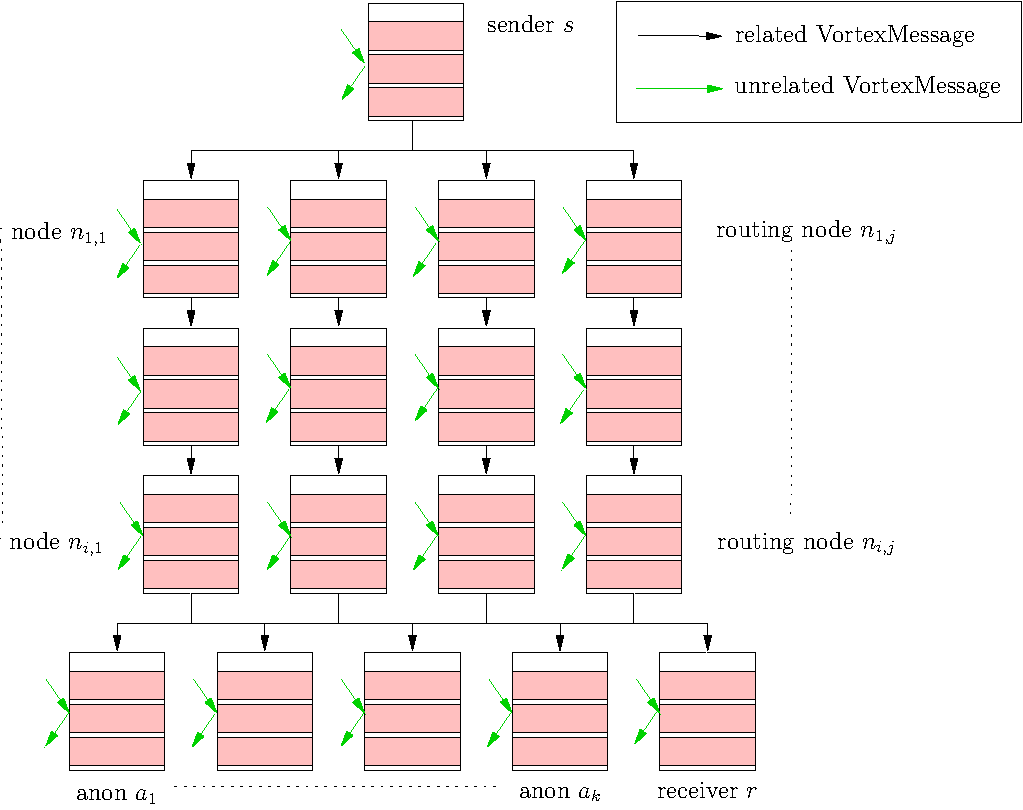
\includegraphics[width=0.7\columnwidth]{inc/messagePaths}
	\caption{A possible path of a VortexMessage}
	\label{fig:messagePaths}
\end{figure}

We have to consider the fact that two adjacent nodes collaborating may build one combined workspace executing all operations. They are, therefore, able to link all operations of these two adjacent nodes and follow all incoming and outgoing paths. We, therefore, may assume that two adjacent nodes or an uninterrupted series of collaborating nodes may be substituted by one node.

So a routing node $n_{1,}$ may not know if a \emph{VortexMessage} received from $s$ is the result of processing another message or the message has been injected on node $s$. Furthermore, if $s$ was acting as a routing node, it successfully unlinked the message from any previous node. The sending node $s$ may send a message by first employing an $addRedundancy$ operation or splitting and encrypting the message. Each path through the streams has then not enough information to rebuild the combined message. If employing an $addRedundancy$ operation, a receiver $r$ may recover a message if sufficient paths through the routing nodes were acting according to the protocol. Paths with misbehaving nodes may eventually be identified depending on the number of redundancy operations. Assuming that the RBB included proper padding Information for the receiver $r$, the receiver may identify what set of \emph{VortexMessages} leads to the original message due to the padding applied before the $RS$ function. So if sufficient paths, depending on the chosen operations at $r$, provide correct data, we may recover nodes misbehaving in our paths. If one node in a path is not collaborating with adjacent nodes in the path, the path of the \emph{VortexMessage} becomes unlinked as previously shown with sender $s$. If multiple paths are used, all paths must have at least one honest node to unlink the message. 

If all nodes in the anonymization set $a_1$\ldots$a_k$ are honest, any preceding node may not know whether the message ends at that node or the message is just routed through an honest node. Even if some of the anonymization nodes are not honest or collaborating with an adversary, the anonymity set may be reduced in size, but the receiver is still part of the anonymity set spanning the honest anonymization nodes. So, we have shown that depending on the chosen routing block, anonymity, unlinkability, and fault tolerance against a misbehaving node may be achieved. AN RBB may furthermore send additional \emph{VortexMessages} to suspected misbehaving nodes. If misbehavior is reproducible within an ephemeral identity, the RBB may identify it by picking up parts of the previously sent message and comparing them to an expected state. An RBB may even introduce message paths leading back to the RBB itself. Such a message path may allow observation of the progress and success of the message delivery.

\subsection{Attacking Anonymity through Timing Analysis}
Timing is under full control of the routing block builder. No information can be derived from the timing. This is even the case if a routing block is reused. The precise timing on the network depends additionally on other factors, such as delaying through anti-UBE or anti-malware measures or delays through local delivery between multiple nodes.

\subsection{Attacking Anonymity through Throughput Analysis}
Increasing the throughput to highlight a message channel is not possible since the replay protection will block such requests. It may be possible for a limited number of times by replaying a MURB. This is one of the reasons why the usage of MURBs is discouraged unless necessary.

\subsection{Attacking Anonymity through Routing Block Analysis}
The routing block is cryptographically secure. The size of the routing block may leak an estimate about its inner complexity. It does not reveal any critical pieces of information like remaining hops to the message end or target or similar.

\subsection{Attacking Anonymity through Header Analysis}
The header contains valuable data that is cryptographically secured and only visible to the next receiver. 

To an adversary not knowing the key, the size of the prefix block may leak the key size. The size of the header block itself may leak the presence of any optional blocks. Besides that, no other information is leaked to such an adversary.

To an adversary knowing the decryption key (evil routing node), the content of the header block is visible. This header block leaks all routing information for the respective node and thus the ephemeral identity. This block leaks some information of minimal value. It may leak the activity of an ephemeral identity, including frequency. This activity is, however, only matching the minimal activity of an endpoint identity as an endpoint may have multiple ephemeral identities on one node. 

\subsection{Attacking Anonymity through Payload Analysis}
The payload itself does not leak any information about the message content. All content is cryptographically secured. Content may, however, leak the block size of the applied cipher.

\subsection{Attacking Anonymity through Bugging}
Bugging is one of the most pressing problems. The protocol has been carefully crafted not to allow any bugging. The use of MIME messages in the final message, however, enables the bugging of the message itself. A bugged message content may breach receiver anonymity to the sender of the message.

\subsection{Attacking Anonymity through Replay Analysis}
Due to the replay protection, no traffic may be generated or multiplied except for the traffic sent by the attacking node. As this information is already known to the node, there is no value in doing so. 

\subsection{Diagnosability of traffic}

\subsubsection{Hijacking of Header and Routing Blocks}
An attacker might try to recombine a header block of the third party with a routing block crafted to get the workspace content of a different node. To protect against this scenario, every routing block and its corresponding header block has a shared value called forwardSecret. As the content of a hijacked header block is not known, he is unable to guess the forward secret within the block.

It is not possible to brute-force the value due to the replay protection. More precisely, the probability of hijacking a single identity block is $\frac{1}{2^{32}}$. Hijacking such a block allows one-time access to the working space and is visible to the owner due to the manipulated quotas. Failing an attack will result in deleting the ephemeral identity, and a new, unlinked ephemeral identity will be created. 

\subsubsection{Partial Implicit Routing Diagnosis}
We can create data that is routed back to or through the original sending node. This traffic is well defined and may be used to certify that the loop processing the message is working as expected. By combining the messages and sending intermediate results through multiple paths, it is even possible to extract the sub status of some loops and combine the result within transfer into a single message.

As a special case, a sender may use implicit routing diagnostic to diagnose the full route. A sender may do this by taking specific excerpts of the received message at the recipients' node and route these blocks back from the recipient to the sender. 

\subsubsection{Partial Explicit Routing Diagnosis}
If a message fails to deliver according to implicitly routing diagnosis, additional messages may be sent to pick up the content of the workspace of ephemeral identities throughout the path. These messages are due to the only binding to the ephemeral identity, not distinguishable from the original messages. Assuming that a node always behaves either according to or not according to the rules of the system, a node may be identified by capturing built blocks with known content.

If a node is identified as a misbehaving node, it may be excluded from subsequent routing requests or reduced in its reliability or trustability ratings. A node may calculate such scores locally to build a more reliable network over time, avoiding misbehaving or non-conformant nodes. This does not violate our zero-trust philosophy as the scoring is made locally and relies on our observations.


\chapter{Analysis of the effectiveness of Attack Schemes}
In the previous sections, we have identified some potential technical weaknesses of the protocol. These weaknesses boil down to the following recommendations:
\begin{itemize}
	\item Avoid using MURBs
	\item Keep workspace (\defref{eID}) lifetime short
	\item 
\end{itemize}

A routing node may further improve the effectiveness of the protocol by...

\begin{itemize}
	\item Create credible decoy content.
	\item Use different addresses on the transport level for sending and receiving.
	\item Use long host keys
\end{itemize}

\chapter{Analysis of Degree of Anonymization in Comparison to other Systems}
It is hard to make a clear statement in terms of anonymity. To allow a comparison, we work with traditional systems of anonymization and compare them to our system and outline the differences.

\section{Comparing \MessageVortex{} to Remailers}
All remailer systems are identifiable due to their traffic.  We leave aside simple remailer types such as nym remailers and concentrate solely on the most advanced type-3 remailer (Mixminion). Although development has been seized, we still can potentially compare the effectiveness of our system compared to a Mixminion system.

Mixminion is an onion routing system working with a fixed message size of 32KB. It relies on a central directory containing all nodes. This is a functionality we can rebuild with \MessageVortex{} by using the $decrypt$ operation. Unlike with the \MessageVortex{} system, Mixminion relies on a public directory. Even compared with a hypothetical system having steganographically hidden services and only locally known routing nodes, our system scores in the following way over a Mixminion router:

\begin{itemize}
	\item No detectability due to timing related constraints.\\
	      Mixminion had no synchronized timing constraints. Messages were sent as soon as the subsequent message node was known and the message decrypted. This behavior makes a node identifiable as it is not a common pattern.
	\item No detectability due to constant sizing of the messages.\\
	      Messages were equally sized into 32KB junks.
	\item No identifiable goal in the case of identified messages by a global observer.\\
		  An observing adversary able to match message sizes may identify messages in a low traffic network and thus identify sender and recipient. 
	\item Possible resistance against a Byzantine node.
	      A Byzantine node would disrupt communication in a Mixminion system. On the other hand, \MessageVortex{} may compensate for such behavior with the possibility of redundant data.
	\item Possibility of redundant routes ($addRedundancy$ operation or just redundant message transfer).\\
	      Messages were assembled according to their sequence number. The possibility of redundant routes is not foreseen in the protocol.
	\item Possibility of monitoring successful delivery.\\
	      Within the Mixminion protocol, there are no means defined to get delivery reports.
	\item Able to build a localized trust relationship for routing nodes over time.\\
	      As we have the possibility to identify successful message delivery within \MessageVortex{}, we may build a localized trust.
\end{itemize}

Both protocols share some common strengths, such as the possibility to specify routing nodes by the sender of a message or the possibilities of reply blocks. 

Having the possibility of mimicking a type 3 remailer and improving the communication scheme makes our system superior to such an improved type 3 remailer. An unmodified type 3 remailer is not capable of working in an environment with n censoring adversary as defined in this work due to its detectability. 

\begin{figure*}[ht]\centering
	\begin{tikzpicture}[node distance=0.5cm,auto,>=stealth]
		\begin{scope}[baseline=(current bounding box.center)]
			\tikzstyle{knode}=[circle,draw=black,thick,inner sep=8pt,baseline=(current bounding box.center)]
			\node[knode] (n-1) at (0:6cm) {recipient};
			\node[knode] (n0) at (0:3cm) {node 3};
			\node[knode] (n1) at (60:3cm) {node 2};
			\node[knode] (n2) at (120:3cm) {node 1};
			\node[knode] (n3) at (180:3cm) {node 0};
			\node[knode] (n4) at (180:6cm) {sender};
			%arrows
			\draw[->] (n-1)--(n0);
			\draw[->] (n0)--(n1);
			\draw[->] (n1)--(n2);
			\draw[->] (n2)--(n3);
			\draw[->] (n3)--(n4);
		\end{scope}
	\end{tikzpicture}
	\caption{A typical Mixminion mix cascade}
	\label{fig:mmCommPattern}
\end{figure*}

\section{Comparing \MessageVortex{} to a DC Network based system}
A DC network may not be built with our \MessageVortex{} protocol. However, if we add a hypothetical $XOR$ operation, we may build such a system. In the early stages of development, we had an $XOR$ operation. When analyzing our system, we were unable to discover good use-cases for such an operation. We assume that the sender and recipient are part of the DC network ring. If not, additional problems regarding entry and exit nodes would prevail. 

When comparing such a hypothetical \MessageVortex{} system with an $XOR$ operation with an again hypothetical DC network using steganographically hidden messages, we conclude that \MessageVortex{} could mimic the behavior of such a network. Making further comparisons along those lines, we have to say that \MessageVortex{} scores in the following ways over such a hypothetical system:

\begin{itemize}
	\item No detectability due to timing related constraints.\\
	      DC networks send messages as an immediate result to the subsequent node. Messages are assumed to be sent as soon as the subsequent message node was known, and the current message has been processed. This behavior makes a node identifiable as it is not a common pattern.
	\item No detectability due to constant sizing of the messages.\\
	      Messages in a DC network may or may not be fixed in sizes. They have, however, a constant size per round. This constant sizing makes involved nodes identifiable.
	\item Possible resistance against a Byzantine node.
	      A Byzantine node would disrupt communication in a standard DC network system. On the other hand, \MessageVortex{} may compensate for such behavior with the possibility of redundant data.
	\item Possibility of redundant routes ($addRedundancy$ operation or just redundant message transfer).\\
	      Messages are transferred as a block. The possibility of redundant routes is typically not foreseen in DC networks.
	\item Possibility of monitoring successful delivery.\\
	      Within DC networks, there are no means defined to have delivery confirmations.
	\item Able to build a localized trust relationship for routing nodes over time.\\
	      As we have the possibility to identify successful message delivery within \MessageVortex{}, we may build a localized trust.
\end{itemize}

Additionally, in a typical DC network, the set of involved nodes is fixed and known. This leads to the problem that the discovery of one network node leads to the full discovery of a ring or even more. If the sender and receiver are not part of the DC network ring but use entry and exit nodes, the discovery of the involved parties is even simpler as a global observer may focus on this node traffic. 

Having the possibility of mimicking a DC network and improving the communication scheme would make our system superior to such an improved DC network. An unmodified DC network is not capable of working in an environment with n censoring adversary as defined in this work due to its detectability. The ring-like communication pattern, as described in \cref{fig:dcCommPattern} is very uncommon in standard internet protocols and thus easily detectable by a global observer. In an environment of an observing adversary, the peer partners may not be anonymous due to their traffic from and to the DC network ring.

\begin{figure*}[ht]\centering
	\begin{tikzpicture}[node distance=0.5cm,auto,>=stealth]
		\begin{scope}[baseline=(current bounding box.center)]
			\tikzstyle{knode}=[circle,draw=black,thick,inner sep=8pt,baseline=(current bounding box.center)]
			\node[knode] (n0) at (0:3cm) {node 0};
			\node[knode] (n1) at (51:3cm) {node 1};
			\node[knode] (n2) at (103:3cm) {node 2};
			\node[knode] (n3) at (154:3cm) {node 3};
			\node[knode] (n4) at (206:3cm) {node 4};
			\node[knode] (n5) at (257:3cm) {node 5};
			\node[knode] (n6) at (309:3cm) {node 6};
			%arrows
			\draw[->] (n0)--(n1);
			\draw[->] (n1)--(n2);
			\draw[->] (n2)--(n3);
			\draw[->] (n3)--(n4);
			\draw[->] (n4)--(n5);
			\draw[->] (n5)--(n6);
			\draw[->] (n6)--(n0);
		\end{scope}
	\end{tikzpicture}
	\caption{A typical DC network communication pattern}
	\label{fig:dcCommPattern}
\end{figure*}


\section{Comparing \MessageVortex{} to a Broadcast-Based System}
A broadcast-based network (BCN) hides a message transfer in such a way that every involved node sends an equally sized message or decoy traffic to all other members of the system. By doing so, they build a full mesh of equally sized messages between all involved nodes, making it impossible to an adversary to identify who was sending message traffic and who was sending a true message. Messages sized bigger than a simple message transmission are split up into multiple messages. Again, we were unable to find a system that does not use an own censorable protocol. We, therefore, assume again a hypothetical BCN piggybacking a common internet protocol. In this part, we make two comparisons: One comparison involving a BCN with only one mesh and a second one with a BCN cascading multiple overlapping BCNs, which we refer to as a cBCN. In both cases, the communication mesh, as shown in \cref{fig:bcCommPattern}, is identifiable as this is a very unusual communication pattern in common internet protocols.

\begin{figure*}[ht]\centering
	\begin{tikzpicture}[node distance=0.5cm,auto,>=stealth]
		\begin{scope}[baseline=(current bounding box.center)]
			\tikzstyle{knode}=[circle,draw=black,thick,inner sep=8pt,baseline=(current bounding box.center)]
			\node[knode] (n0) at (0:3cm) {node 0};
			\node[knode] (n1) at (51:3cm) {node 1};
			\node[knode] (n2) at (103:3cm) {node 2};
			\node[knode] (n3) at (154:3cm) {node 3};
			\node[knode] (n4) at (206:3cm) {node 4};
			\node[knode] (n5) at (257:3cm) {node 5};
			\node[knode] (n6) at (309:3cm) {node 6};
			%arrows
			\draw[->] (n0)--(n1);
			\draw[->] (n0)--(n2);
			\draw[->] (n0)--(n3);
			\draw[->] (n0)--(n4);
			\draw[->] (n0)--(n5);
			\draw[->] (n0)--(n6);
			\draw[->] (n1)--(n0);
			\draw[->] (n1)--(n2);
			\draw[->] (n1)--(n3);
			\draw[->] (n1)--(n4);
			\draw[->] (n1)--(n5);
			\draw[->] (n1)--(n6);
			\draw[->] (n2)--(n0);
			\draw[->] (n2)--(n1);
			\draw[->] (n2)--(n3);
			\draw[->] (n2)--(n4);
			\draw[->] (n2)--(n5);
			\draw[->] (n2)--(n6);
			\draw[->] (n3)--(n0);
			\draw[->] (n3)--(n1);
			\draw[->] (n3)--(n2);
			\draw[->] (n3)--(n4);
			\draw[->] (n3)--(n5);
			\draw[->] (n3)--(n6);
			\draw[->] (n4)--(n0);
			\draw[->] (n4)--(n1);
			\draw[->] (n4)--(n2);
			\draw[->] (n4)--(n3);
			\draw[->] (n4)--(n5);
			\draw[->] (n4)--(n6);
			\draw[->] (n5)--(n0);
			\draw[->] (n5)--(n1);
			\draw[->] (n5)--(n2);
			\draw[->] (n5)--(n3);
			\draw[->] (n5)--(n4);
			\draw[->] (n5)--(n6);
			\draw[->] (n6)--(n0);
			\draw[->] (n6)--(n1);
			\draw[->] (n6)--(n2);
			\draw[->] (n6)--(n3);
			\draw[->] (n6)--(n4);
			\draw[->] (n6)--(n5);
		\end{scope}
	\end{tikzpicture}
	\caption{A typical broadcast network communication pattern (full mesh)}
	\label{fig:bcCommPattern}
\end{figure*}

A BCN is a high load network having a very suspicious and uncommon communication pattern within internet protocols. \MessageVortex{} may rebuild such behavior by crafting routing blocks that trigger such a message pattern. Assuming no overlapping pattern, it would always expose the sending node as the first node sending a message. In such a case, privacy would be equal with a single one peer broadcast, as shown in \cref{fig:bcRedCommPattern}. When assuming an overlapping pattern, a first node is no longer identifiable when using a full mesh in the case of a \VortexMessage{}. Atom\cite{kwon2016atom} cascades multiple BCNs into a cBCN. To achieve a cBCN, Atom relies on a central directory infrastructure. Additionally, to a simple BCN, Atom offers zero-knowledge proofs.

\begin{figure*}[ht]\centering
	\begin{tikzpicture}[node distance=0.5cm,auto,>=stealth]
		\begin{scope}[baseline=(current bounding box.center)]
			\tikzstyle{knode}=[circle,draw=black,thick,inner sep=8pt,baseline=(current bounding box.center)]
			\node[knode] (n0) at (0:3cm) {node 0};
			\node[knode] (n1) at (51:3cm) {node 1};
			\node[knode] (n2) at (103:3cm) {node 2};
			\node[knode] (n3) at (154:3cm) {node 3};
			\node[knode] (n4) at (206:3cm) {node 4};
			\node[knode] (n5) at (257:3cm) {node 5};
			\node[knode] (n6) at (309:3cm) {node 6};
			%arrows
			\draw[->] (n0)--(n1);
			\draw[->] (n0)--(n2);
			\draw[->] (n0)--(n3);
			\draw[->] (n0)--(n4);
			\draw[->] (n0)--(n5);
			\draw[->] (n0)--(n6);
		\end{scope}
	\end{tikzpicture}
	\caption{A reduced broadcast network communication pattern (single broadcast)}
	\label{fig:bcRedCommPattern}
\end{figure*}

In the following section, we compare \MessageVortex{} mimicking a BCN to a traditional BCN. We assume again that the transport layer is steganographically secured comparable to \MessageVortex.

In such a case, we may conclude that \MessageVortex{} scores over a BCN...
\begin{itemize}
	\item Equal detectability due to timing related constraints.\\
	      If \MessageVortex{} is mimicking a BCN, timing is essential. Therefore, detectability remains the same for both systems. We could argue that a \MessageVortex{} could mimic an adapted version of a BCN not working in epochs and just mimicking the communication pattern. While this would make a difference in traceability, it does not affect detectability in a positive or negative manner.
	\item No detectability due to constant sizing of the messages.\\
	      Traditional BCNs have fixed message sizes. \MessageVortex{} may mimic the communication pattern with or without such a restriction. The message size may not leak any properties when using \MessageVortex{}. Messages may travel in parts or as a whole piece.
	\item Possible resistance against a Byzantine node.
	      A Byzantine node may disrupt communication in a standard BCN by flooding the network. On the other hand, \MessageVortex{} may compensate for such behavior with the possibility of redundant data. If we assume that a Byzantine node is not flooding the network completely, it is very likely that a BCN is more robust than a network of \VortexNodes{}. A BCN will score at least better if the direct path between the sender and recipient is not affected by the Byzantine node. 
	\item Possibility of redundant routes ($addRedundancy$ operation or just redundant message transfer).\\
	      Messages are transferred as a block. The possibility of redundant routes is typically not foreseen in a BCN.
	\item Possibility of monitoring successful delivery.\\
          By default, a node has no means to observe successful delivery in a BCN. Using \MessageVortex{}, we may do this either by implicit or explicit diagnostic covering one or more epochs.
	\item Able to build a localized trust relationship for routing nodes over time.\\
	      As we have the possibility to identify successful message delivery within \MessageVortex{}, we may build a localized trust. A traditional BCN lacks this possibility. Extended networks such as ATOM may surpass this limitation.
\end{itemize}

To conclude, \MessageVortex{} may offer at least the same properties as a BCN or cBCN. Unlike Atom, it is unable to offer zero-knowledge proofs. As an alternative, \MessageVortex{} offers diagnostics. By using multi-path message transfer, \MessageVortex{} may reduce bandwidth waste and improve throughput. These capabilities of \MessageVortex{} come at the price of local node storage, complex routing operations, and RBB strategies. On the other hand, processing and scalability of \MessageVortex{} do surpass Atoms' capability by far as the rather complex processing of Atom is very limiting.

\chapter{Recommendations on Using the Vortex Protocol}
The following sections list recommendations using the \MessageVortex{} protocol. It is a summary of the previous sections.

\section{Reuse of Routing blocks\label{sec:reuseRB}}
Routing blocks should not be reused. The reuse of a routing block may leak some limited information to an adversary node, such as approximate message size or message frequency of an unknown tupel using this network.

\section{Use of Ephemeral Identities}
Ephemeral identities should be used for a minimal number of messages. Using multiple identities with overlapping lifespans is considered a good practice. Using different ephemeral identities for the same message is acceptable and can be a good practice as long as operations do not leak the linking between those two identities.

Special care must be taken if using overlapping ephemeral identities across nodes. While ephemeral identities may be completely unlinked on a single node, the linking between multiple nodes may leave a trace from one identity to the next. It is advisable to recreate on a regular basis all ephemeral identities from scratch. This guarantees an unlinking from previous ephemeral identities.

\section{Recommendations on Operations applied on Nodes}
All operations carried out on a single node have to be crafted in such a way that no information whether the operation is a decoy or a real message is leaked. Otherwise, it becomes possible to narrow down the message flow.

Encryption operations should be either strictly encrypting or strictly decrypting. At no point in the path, a previously applied encryption on an untrusted node should be removed as removal might lead to linking to the previous inverse operation.

Similarly, there are rules for adding and removing redundancy information. As these operations serve as decoy traffic generators, great care needs to be taken not to leak this information. We emphasize here again that it is possible to add redundancy information on one node, encrypt one or multiple blocks once, or multiple blocks on a second node, and then remove the redundancy information again from the new set. This will lead to a payload data block than the original. However, this does not qualify the block as decoy traffic. The process may be reversed on the final recipient. Such an operation is, however, mathematically very demanding if the same operation is used for redundancy at the same time as multiple possible tuples need to be tried if one node has failed.

Whenever possible, the reappearance of a payload block in a single encoding it should be avoided or limited to an absolute minimum as such an occurrence allows linking of two ephemeral identities.

\section{Reuse of Keys, IVs, or Routing Patterns}
An RBB should avoid reuse of any keys, IVs, routing patterns, or PRNG seeds along its routing path of untrusted nodes. Reusing such values would allow an attacker to match ephemeral identities to a single identity. While this is minimal risk and may be ignored in some cases, an RBB should avoid it as it may leak information to collaborating nodes.

\section{Recommendations on Choosing involved Nodes}
Involved nodes should be trustworthy but not necessarily trusted. A message should always include a set of known recipients. It is regarded as a good practice to use a minimal fixed anonymity set of known recipients as routers. Doing so does not leak any information unless always the same pattern of operations is applied (see \cref{sec:reuseRB}).

\section{Message content}
Although it is possible to embed any content into a Vortex message, great care should be taken as the content may allow disclosing a reader's identity or location. For this reason, only self-contained messages should be used (such as plain text messages).

Allowing a user to use more complex representations such as MIME offers many possibilities for the bugging of the content. A client displaying such messages should always handle them with great care. Taping messages by downloading external images or verifying the validity by OCSP, or even doing a reverse lookup on an IP address may leak valuable information.

\subsection{Splitting of message content}
Message content should be split and distributed among routing nodes. Splitting should, however, not be done excessively to avoid failure due to too many failing nodes. It furthermore makes diagnostics complicated. 

\section{Routing}
The basics of routing is described in \cref{sec:routingLayer}
\subsection{Redundancy}
Redundancy is a valuable feature of the protocol. It allows unsuspicious decoy generation and to compensate message path disruption. A routing block should always be crafted in such a way that redundancy is aligned with the complexity of the routing block and the importance of a message to avoid an adversary controlling all nodes except for the sender's and receiver's one.

\subsection{Operation Considerations}
Operations should be kept easy, but at the same time, guarantee anonymity. The following recommendations are kept to an absolute minimum in order not to create any identifiable behavior.

A payload block should always have a single representation only once when traveling through routing nodes. A recurring pattern would allow an evil router to identify and thus match an ephemeral identity of one router to an ephemeral identity of another router even if there are multiple routes in between. So, when applying encryption only operations between routing nodes, the encryption should be onionized. A clear onionizing routing pattern (only showing encryption steps on a single chunk) is OK. A pattern such as removing encryption and then reapply different encryption is not.

\subsection{Anonymity}
Anonymity is greatly dependent on the quality of the routing block and the chosen anonymity set for a single message and a communication tuple over time. 

\subsubsection{Size of the Anonymity Set}
The requirement for an anonymity set is dependent on jurisdictional restrictions. In some of the more restrictive countries, no one can be held guilty for an action that may not be credibly assigned to him alone. In other jurisdictions, it is possible to be held liable for actions just because of an identified membership in a group. This makes it essential that message traffic and the crafting of the blending is under the sole control of the sender. He needs to create an anonymity-set sufficiently large and spanning enough jurisdictions to create sufficient anonymity for his situation.

  
  
  
  
  
  

%!TeX program=pdflatex
%!TeX encoding=utf8
%!TeX spellcheck = en_US
%!TeX root = ../../messageVortex.tex
\partepigraph{Limit your inputs to only those that support a certain kind of self-destructive behavior, and you can be cheered with enthusiasm as you drive yourself off a cliff.}{Adam-Troy Castro}
\part{Discussion on Results}
\fxwarning{complete section}

\chapter{Measuring up to the Requirenets\label{sec:reqDiscussion}}
In this section we analyze the level of achievment in respect to the requirements defined in section\ref{sec:requirements}. We will go through each requirement and discuss the level of achievement. In the case of a failure, we highlight the reason for the failure and elaborate on the consequences of the current flaws.

\fxwarning{complete section}


\chapter{Achieved level of anonymity}
\fxwarning{complete section}

\chapter{Weaknesses of the protocol}
\fxwarning{complete section}

\chapter{Further and Missing Research}
\fxwarning{complete section}

\appendix

%!TeX program=pdflatex
%!TeX encoding=utf8
%!TeX spellcheck = en_US
%!TeX root = ../../messageVortex.tex

\part{Appendix}

\onecolumn
%\appendix
\pagenumbering{arabic}% resets `page` counter to 1
\renewcommand*{\thepage}{A\arabic{page}}
%\renewcommand{\setthechapter}{\Alph{section}}
%\renewcommand\thechapter{\Alph{chapter}}
\setcounter{chapter}{0}


\gdef\rfc{../../../../rfc/src/xml2rfc/draft-gwerder-messagevortexmain-08.pdf}
%\includepdf[pages=-,frame=true,scale=0.5]{\rfc}
\includepdf[pages=1,frame=true,scale=0.70,pagecommand={\chapter{The RFC draft document\label{app:rfcMessageVortexMain}}}, offset=0 -1cm]{\rfc}
\includepdf[pages=2-,frame=true,scale=0.8,pagecommand={}, offset=0 -1cm]{\rfc}

\clearpage\chapter{Glossary}

\begin{entry}
	\mainentry{adversary}{In this work, we referr to an adversary as any entity opposing to the privacy of a message. For a more throughout definition, refer to section~\ref{sec:adversary}}
\end{entry}

\begin{entry}
	\mainentry{anonymity}{We refer to the term anonymity as defined in \cite{anonTerminology}. ``Anonymity of a subject means that the subject is not identifiable within a set of subjects, the anonymity set.''\omitted}
	\subentry{Sender Anonymity}{The anonymity set is the set of all possible subjects. For actors, the anonymity set consists of the subjects who might cause an action. For actees, the anonymity set consists of the subjects which might be acted upon. Therefore, a sender may be anonymous (sender anonymity) only within a set of potential senders, his/her sender anonymity set, which itself may be a subset of all subjects worldwide who may send a message from time to time.}
	\subentry{Receiver Anonymity}{The same for the recipient means that a recipient may be anonymous (recipient anonymity) only within a set of potential recipients, his/her recipient anonymity set. Both anonymity sets may be disjoint, be the same, or they may overlap. The anonymity sets may vary over time.}
\end{entry}

\begin{entry}
	\mainentry{agent}{An agent is a single component of a \defref{service} provided to a user or other services.}
\end{entry}


\begin{entry}
	\mainentry{carrier message}{A transport layer message containing an embedded \VortexMessage. In an ideal implementation a carrier message is not identifiable as a carrier of a \VortexMessage.}
\end{entry}

\begin{entry}
	\mainentry{decoy traffic}{Any data transported between routers that have no relevance to the message at the final destination and are not needed for the flow of the message.}
\end{entry}

\begin{entry}
	\mainentry{eID}{An ephemeral identity (eID) is a unique user of a \VortexNode{} characterized by its public key. This user is created with a \VortexMessage{} and has only a limited lifetime. After expiry all informations related to this identity are deleted.}
\end{entry}

\begin{entry}
	\mainentry{EWS}{Exchange Web Services (EWS) are a Microsoft proprietary protocol to access exchange services from a client. It may be regarded as an alternative to IMAPv4. This is, however, incomplete as EWS offers additional features such as User Configuration, Delegate Management or Unified Messaging.}
\end{entry}

\begin{entry}
	\mainentry{identity}{A tuple of a routable address and a public key. This tuple is a long-living tuple but may be exchanged from time to time. An Identity is always assigned to a node, but one node may have multiple identities.}
\end{entry}

\begin{entry}
	\mainentry{jurisdiction}{A geographical area where a set of legal rules created by a single actor or a group of actors apply, which contains executive capabilities (e.g., police, army, or secret service) to enforce this set of legal rules. Most of these legal rules are based on their specific physical location (e.g., German law is limited to the jurisdiction of Germany). Some jurisdictions may over-arch multiple separated geographical locations (e.g., laws of the European Union) or specific to some handpicked countries (e.g., International Covenant on Civil and Political Rights). Due to their overlapping nature, multiple jurisdictions may have contradictory rules applying for the same event.}
\end{entry}

\begin{entry}
	\mainentry{IMAP}{IMAP (currently IMAPv4) is a typical protocol used between a \defref{Client MRA} and a \defref{Remote MDA}. It has been specified in its current version in \cite{rfc3501}. The protocol is capable of fully maintaining a server-based message store. This includes the capability of adding, modifying, and deleting messages and folders of a mailstore. It does not include, however, sending emails to other destinations outside the server-based store.}
\end{entry}

\begin{entry}
	\mainentry{ID}{A numerical identification reflecting a single payload chunk in a \defref{workspace} of an \defref{eID}.}
\end{entry}

\begin{entry}
	\mainentry{IoI}{The Item of Intrest (IoI) are defined in \cite{anonTerminology} and refer to any subject action or entity which is of interest to a potential adversary.}
\end{entry}

\begin{entry}
	\mainentry{LMTP}{The Local Mail Transfer Protocol is defined in \cite{rfc2033}. This RFC defines a protocol similar to SMTP for local mail senders. This protocol allows a sender to have no mail queue at all and thus simplifies the client implementation.}
\end{entry}

\begin{entry}
	\mainentry{local mail store}{A Local Mail Store offers a persistent store on a local non-volatile memory in which messages are being stored. A store may be flat or structured (e.g., supports folders). A local mail store may be an authoritative store for mails or a ``cache only'' copy. It is typically not a queue.}
\end{entry}

\begin{entry}
	\mainentry{MDA}{An MDA provides uniform access to a local message store.}
	\subentry{Remote MDA}{A Remote MDA typically supports a specific access protocol to access the data stored within a local message store.}
	\subentry{Local MDA}{A Local MDA typically gives local applications access to a server store. This may be done through an API, a named socket, or similar mechanisms.}
\end{entry}

\begin{entry}
	\mainentry{message}{The ``real content'' to be transferred from the sender to the recipient. Please note the difference compared to a \VortexMessage. We refer to the encoded form of a \VortexMessage, which may or may not contain parts of the original message always as \VortexMessage.}
\end{entry}

\begin{entry}
	\mainentry{MessageVortex}{The protocol described in this document.}
\end{entry}

\begin{entry}
	\mainentry{MRA}{A Mail Receiving Agent is an agent, which receives emails from another agent. Depending on the used protocol, two subtypes of MRAs are available.}
	\subentry{Client MRA}{A client MRA picks up emails in the server mail storage from a remote MDA. Client MRAs usually connect through a standard protocol that was designed for client access. Examples for such protocols are POP or IMAP.}
	\subentry{Server MRA}{Unlike a client MRA, a server MRA listens passively for incoming connections and forwards received messages to an MTA for delivery and routing. A typical protocol supported by a server MRA is SMTP}
\end{entry}

\begin{entry}
	\mainentry{MS-OXCMAPIHTTP}{Microsofts Messaging Application Programming Interface (MAPI) 
		Extensions for HTTP specifies the Messaging Application Programming Interface (MAPI) Extensions for HTTP in \cite{ms-oxcmapihttp}, which enable a client to access personal messaging and directory data on a server by sending HTTP requests and receiving responses returned on the same HTTP connection. This protocol extends HTTP and HTTPS.}
\end{entry}

\begin{entry}
	\mainentry{MSA}{A Mail Sending Agent. This agent sends emails to a \defref{Server MRA}. }
\end{entry}

\begin{entry}
	\mainentry{MTA}{A Mail Transfer Agent. This transfer agent routes emails between other components. Typically an MTA receives emails from an MRA and forwards them to an MDA or MSA. The main task of an MTA is to provide reliable queues and solid track of all emails as long as they are not forwarded to another MTA or local storage.}
\end{entry}

\begin{entry}
	\mainentry{MTS}{A Mail Transfer Service. This is a set of agents that provide the functionality to send and receive messages and forward them to a local or remote store.}
\end{entry}

\begin{entry}
	\mainentry{MSS}{A Mail Storage Service. This is a set of agents providing a reliable store for local mail accounts. It also provides interfacing, which enables clients to access the users' mail.}
\end{entry}

\begin{entry}
	\mainentry{MUA}{A Mail User Agent. This user-agent reads emails from local storage and allows a user to read existing emails, create and modify emails.}
\end{entry}

\begin{entry}
	\mainentry{MURB}{A multi-use reply block. This type of routing block is provided by a sender to give a node the possibility to route back answers without the knowledge of the location of the sender. In contrast to a SURB, a MURB may be used multiple times. The number of times is regulated by the $maxReplay$ field. Furthermore, a MURB must provide multiple peer keys for all routing steps to avoid repeating patterns of key blocks. This structure makes a MURB much larger than a SURB.}
\end{entry}

\begin{entry}
	\mainentry{operation}{A function transforming the content of a \defref{payload block}. \MessageVortex{} supports four categories of operations. Relevant for the service are $addRedundancy$/$removeRedundancy$, $encrypt$/$decrypt$, and $split$/$merge$. Additionally for operations there is a $mapping$ operation allowing to map the payloads of a message into the payload space or vice-versa.}
\end{entry}

\begin{entry}
\mainentry{payload}{Any data transported between routers regardless of the meaningfulness or relevance to the \VortexMessage.}
\end{entry}

\begin{entry}
\mainentry{payload block}{A single block attached to a \VortexMessage{} representing either the message or the decoy content.}
\end{entry}

\begin{entry}
\mainentry{privacy}{From the Oxford English Dictionary: ``
	\begin{enumerate}
		\item The state or condition of being withdrawn from the society of others, or from the public interest; seclusion. The state or condition of being alone, undisturbed, or free from public attention, as a matter of choice or right; freedom from interference or intrusion.
		\item Private or retired place; private apartments; places of retreat.
		\item Absence or avoidance of publicity or display; a condition approaching to secrecy or concealment. Keeping of a secret.
		\item A private matter, a secret; private or personal matters or relations; The private parts.
		\item Intimacy, confidential relations.
		\item The state of being privy to some act.
	\end{enumerate}''\cite{OXFORD}\\
	In this work, privacy is related to definition two. Mails should be able to be handled as a virtual private place where no one knows who is talking to whom and about what or how frequent (except for directly involved people).
}
\end{entry}

\begin{entry}
\mainentry{pseudonymity}{
	As Pseudonymity we take the definition as specified in \cite{anonTerminology}.
	\begin{shadequote}{}
		A pseudonym is an identifier of a subject other than one of the subject's real names. The subject which the pseudonym refers to is the holder of the pseudonym. A subject is pseudonymous if a pseudonym is used as an identifier instead of one of its real names.\omitted
	\end{shadequote}
}
\end{entry}

\begin{entry}
\mainentry{POP}{POP (currently in version 3) is a typical protocol to be used between a \defref{Client MRA} and a \defref{Remote MDA}. Unlike \defref{IMAP}, it is not able to maintain a mail store. Its sole purpose is to fetch and delete emails in a server-based store. Modifying Mails or even handling a complex folder structure is not feasible with POP}.
\end{entry}

\begin{entry}
\mainentry{recipient}{The user or process destined to receive the message in the end.}
\end{entry}

\begin{entry}
\mainentry{router}{Any \VortexNode which is processing messages. Please note that all \VortexNodes are routers.}
\end{entry}

\begin{entry}
\mainentry{routing block}{A block in the \VortexMessage containing all the instructions for processing the current message. It may furthermore contain additional routing blocks to compose subsequent messages. The routing block is protected by the sender key $K_{sender}$.}
\end{entry}

\begin{entry}
\mainentry{routing graph}{A graphical representation of a \defref{routing block}. A routing graph is a directed multigraph with \VortexNodes{} as nodes and \VortexMessages{} as edges. For further details see section~\ref{sec:routingGraph}.}
\end{entry}

\begin{entry}
\mainentry{RBB}{A routing block builder (RBB) is a \VortexNode{} assembling the operations and hops for a message. If the RBB is not equal to the sender of the message, the receiver may be anonymous to the sender.}
\end{entry}

\begin{entry}
\mainentry{sender}{The user or process originally composing the message. We refer as the sender to both the human creator or initiator of a message, as well as the process of assembling and preparing the message.
	\subentry{immediate sender}{The actually peering sender. This is the sender which sent the current message.}
}
\end{entry}

\begin{entry}
\mainentry{server admin}{We regard a server admin as a person with high privileges and profound technical knowledge of a server and its associated technology. A server admin may have access to one or multiple servers of the same kind.}
\end{entry}

\begin{entry}
\mainentry{service}{A service is an endpoint on a server providing the functionality to a client. This service may consist of several agents (\defref{agent}).}
\end{entry}

\begin{entry}
\mainentry{SMTP}{SMTP is the most commonly used protocol for sending emails across the Internet. In its current version it has been specified in \cite{rfc5321}.}
\end{entry}

\begin{entry}
\mainentry{storage}{A store to keep data. It is assumed to be temporary or persistent.}
\end{entry}

\begin{entry}
\mainentry{SURB}{A single-use reply block. This type of routing block is provided by a sender to give a node the possibility to route back answers without the knowledge of the location of the sender. A SURB may only be used once subsequent uses of the block are not possible. The lifetime of a SURB is typically limited to minutes or hours.}
\end{entry}

\begin{entry}
\mainentry{UBM}{We use the term Unsolicited Bulk Message as a term for any mass message being received by a user without prior explicit consent. A less formal term for such a message in email terminology is spam or junk mail.}
\end{entry}

\begin{entry}
\mainentry{undetectability}{
	As undetectability we take the definition as specified in \cite{anonTerminology}.
	\begin{shadequote}{}
		Undetectability of an item of interest (IOI\index{Item of Interest}) from an attacker's perspective means that the
		attacker cannot sufficiently distinguish whether it exists or not.\omitted
	\end{shadequote}
}
\end{entry}

\begin{entry}
\mainentry{unlikability}{We refer to the term unlinkability as defined in \cite{anonTerminology}. ``Unlinkability of two or more items of interest (IOIs, e.g., subjects, messages, actions, ...) from an attacker’s perspective means that within the system (comprising these and possibly other items), the attacker cannot sufficiently distinguish whether these IOIs are 
	related or not.}
\end{entry}

\begin{entry}
\mainentry{unobservability}{
	As unobservability we take the definition as specified in \cite{anonTerminology}.
	\begin{shadequote}{}
		Unobservability of an item of interest (IOI) means
		\begin{itemize}
			\item undetectability of the IOI against all subjects uninvolved in it and
			\item anonymity of the subject(s) involved in the IOI even against the other subject(s) involved in that IOI.
		\end{itemize}
	\end{shadequote}        
	As mentioned in this paper, unobservability raises the bar of required attributes again ($\Rightarrow$ reads ``implies''):
	\begin{eqnarray*}
		censorship\ resistance & \Rightarrow & unobservability\\
		unobserability         & \Rightarrow & undetectability\\
		unobserability         & \Rightarrow & anonymity
	\end{eqnarray*}
}
\end{entry}


\begin{entry}
\mainentry{user}{Any entity operating a \VortexNode.}
\end{entry}

\begin{entry}
\mainentry{VortexMessage}{The encoded message passed from one \VortexNode{} to another. The \VortexMessage{} is typically considered before any embedding takes place.}
\end{entry}

\begin{entry}
\mainentry{VortexNode}{A hardware node running the \MessageVortex{} specific software. These nodes typically run on always-connected, user-run devices such as mobile phones or tablets.}
\end{entry}

\begin{entry}
\mainentry{workspace}{A storage uniquely allocated for a specific \defref{eID}. Within this workspace, we find all received payloads referred by an \defref{ID}, all routing blocks to be processed, and all unexpired \defref{operation}s.}
\end{entry}

\begin{entry}
\mainentry{XMPP}{The Extensible Messaging and Presence Protocol (XMPP)\cite{rfc6120,rfc6121} was formerly also known as Jabber protocol. It is an extensible instant messenger protocol widely adopted in chat clients.}
\end{entry}

\begin{entry}
\mainentry{zero trust}{
	Zero trust is not a truly researched model in systems engineering. It is, however, widely adopted. We refer in this work to the zero trust model when denying the trust in any infrastructure not directly controlled by the sending or receiving entity. This distrust extends especially but not exclusively to the network transporting the message, the nodes storing and forwarding messages, the backup taken from any system except the client machines of the sending and receiving parties, and software, hardware, and operators of all systems not explicitly trusted. As explicitly trusted in our model, we do regard the user sending a message (and his immediate hardware used for sending the message) and the users receiving the messages. Trust in between the receiving parties (if more than one) of a message is not necessarily given.
}
\end{entry}        

\backmatter
\refstepcounter{chapter}
\chapter{Bibliography}
{
%\def\filespliter#1{\expandafter\intfilespliter#1\relax}
%\def\intfilespliter#1 #2 #3\relax{ First: (#1), Second: (#2), Third: (#3) }
\printbibliography[title={},heading=none]
}

% additional reference entries
\index{mail transport|see {message transport}}
\index{Jabber|see {XMPP}}

% add the index
\refstepcounter{chapter}
\clearpage\printindex

%\clearpage\chapter{Short Biography}
%\begin{wrapfigure}{R}{0.3\columnwidth}
%\includegraphics[width=0.29\columnwidth]{inc/biography/passphoto}
%\end{wrapfigure}
%% !TeX spellcheck = en_GB

Martin Gwerder was born 20. July 1972 in Glarus, Switzerland. He is currently a doctoral Student at the University of Basel. After having concluded his studies at the polytechnic at Brugg in 1997, he did a postgraduate study as a master of business and engineering. Following that, he changed to the university track doing an MSc in Informatics at FernUniversit\"at in Hagen. While doing this he constantly broadened his horizon by working for industry, banking and government as  engineer and architect in security related positions. He currently holds a lecturer position for cloud and security at the University of Applied Sciences Northwestern Switzerland. His main expertise lays in the field of networking related problems dealing with data protection, distribution, confidentiality and anonymity.

\cleardoublepage~\clearpage
\end{document}